\pagebreak
\thispagestyle{empty}
\floatpagestyle{empty}

\movetoevenpage
\thispagestyle{empty}
%\begin{absolutelynopagebreak}
\begin{vplace}
\begin{figure}[H]
%\begin{adjustwidth}{-1.9cm}{}
  %\vspace*{4.25cm}
  \hspace*{-1cm}
  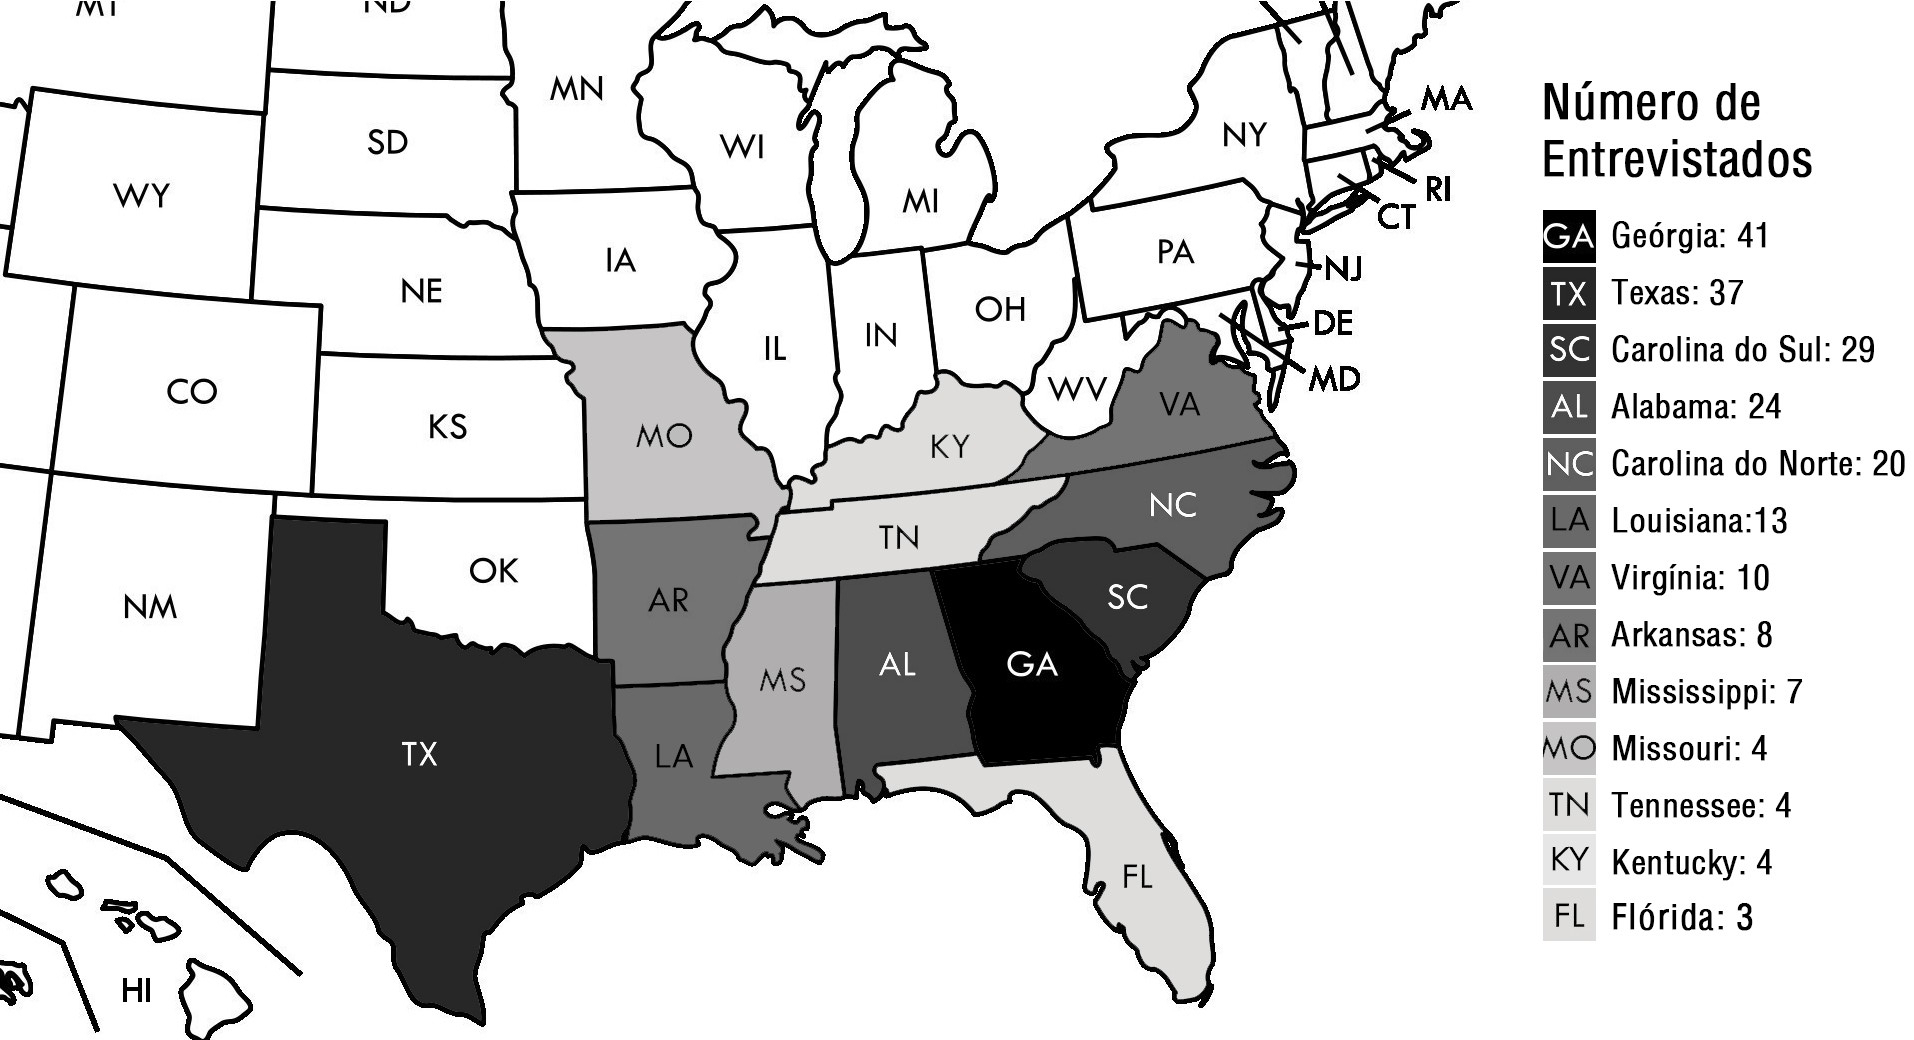
\includegraphics[width=120mm]{./imgs/mapa1.jpg}  
  %\hfill
%\end{adjustwidth}
  \caption{Estados do sul dos Estados Unidos onde os entrevistados viveram a escravidão}
\end{figure}
\end{vplace}

%\end{absolutelynopagebreak}

\chapter*{}
\addcontentsline{toc}{part}{Nascidos na escravidão}
\begin{center}
\begin{vplace}[0.3]
\Large
Nascidos na escravidão
\end{vplace}
\end{center}
\thispagestyle{empty}

\pagebreak
\thispagestyle{empty}

\begin{absolutelynopagebreak}
\begin{vplace}
\begin{figure}[H]
\begin{adjustwidth}{-1.8cm}{}
  %\centering
  \vspace*{-2cm}
  %\hspace{-0.5cm}
  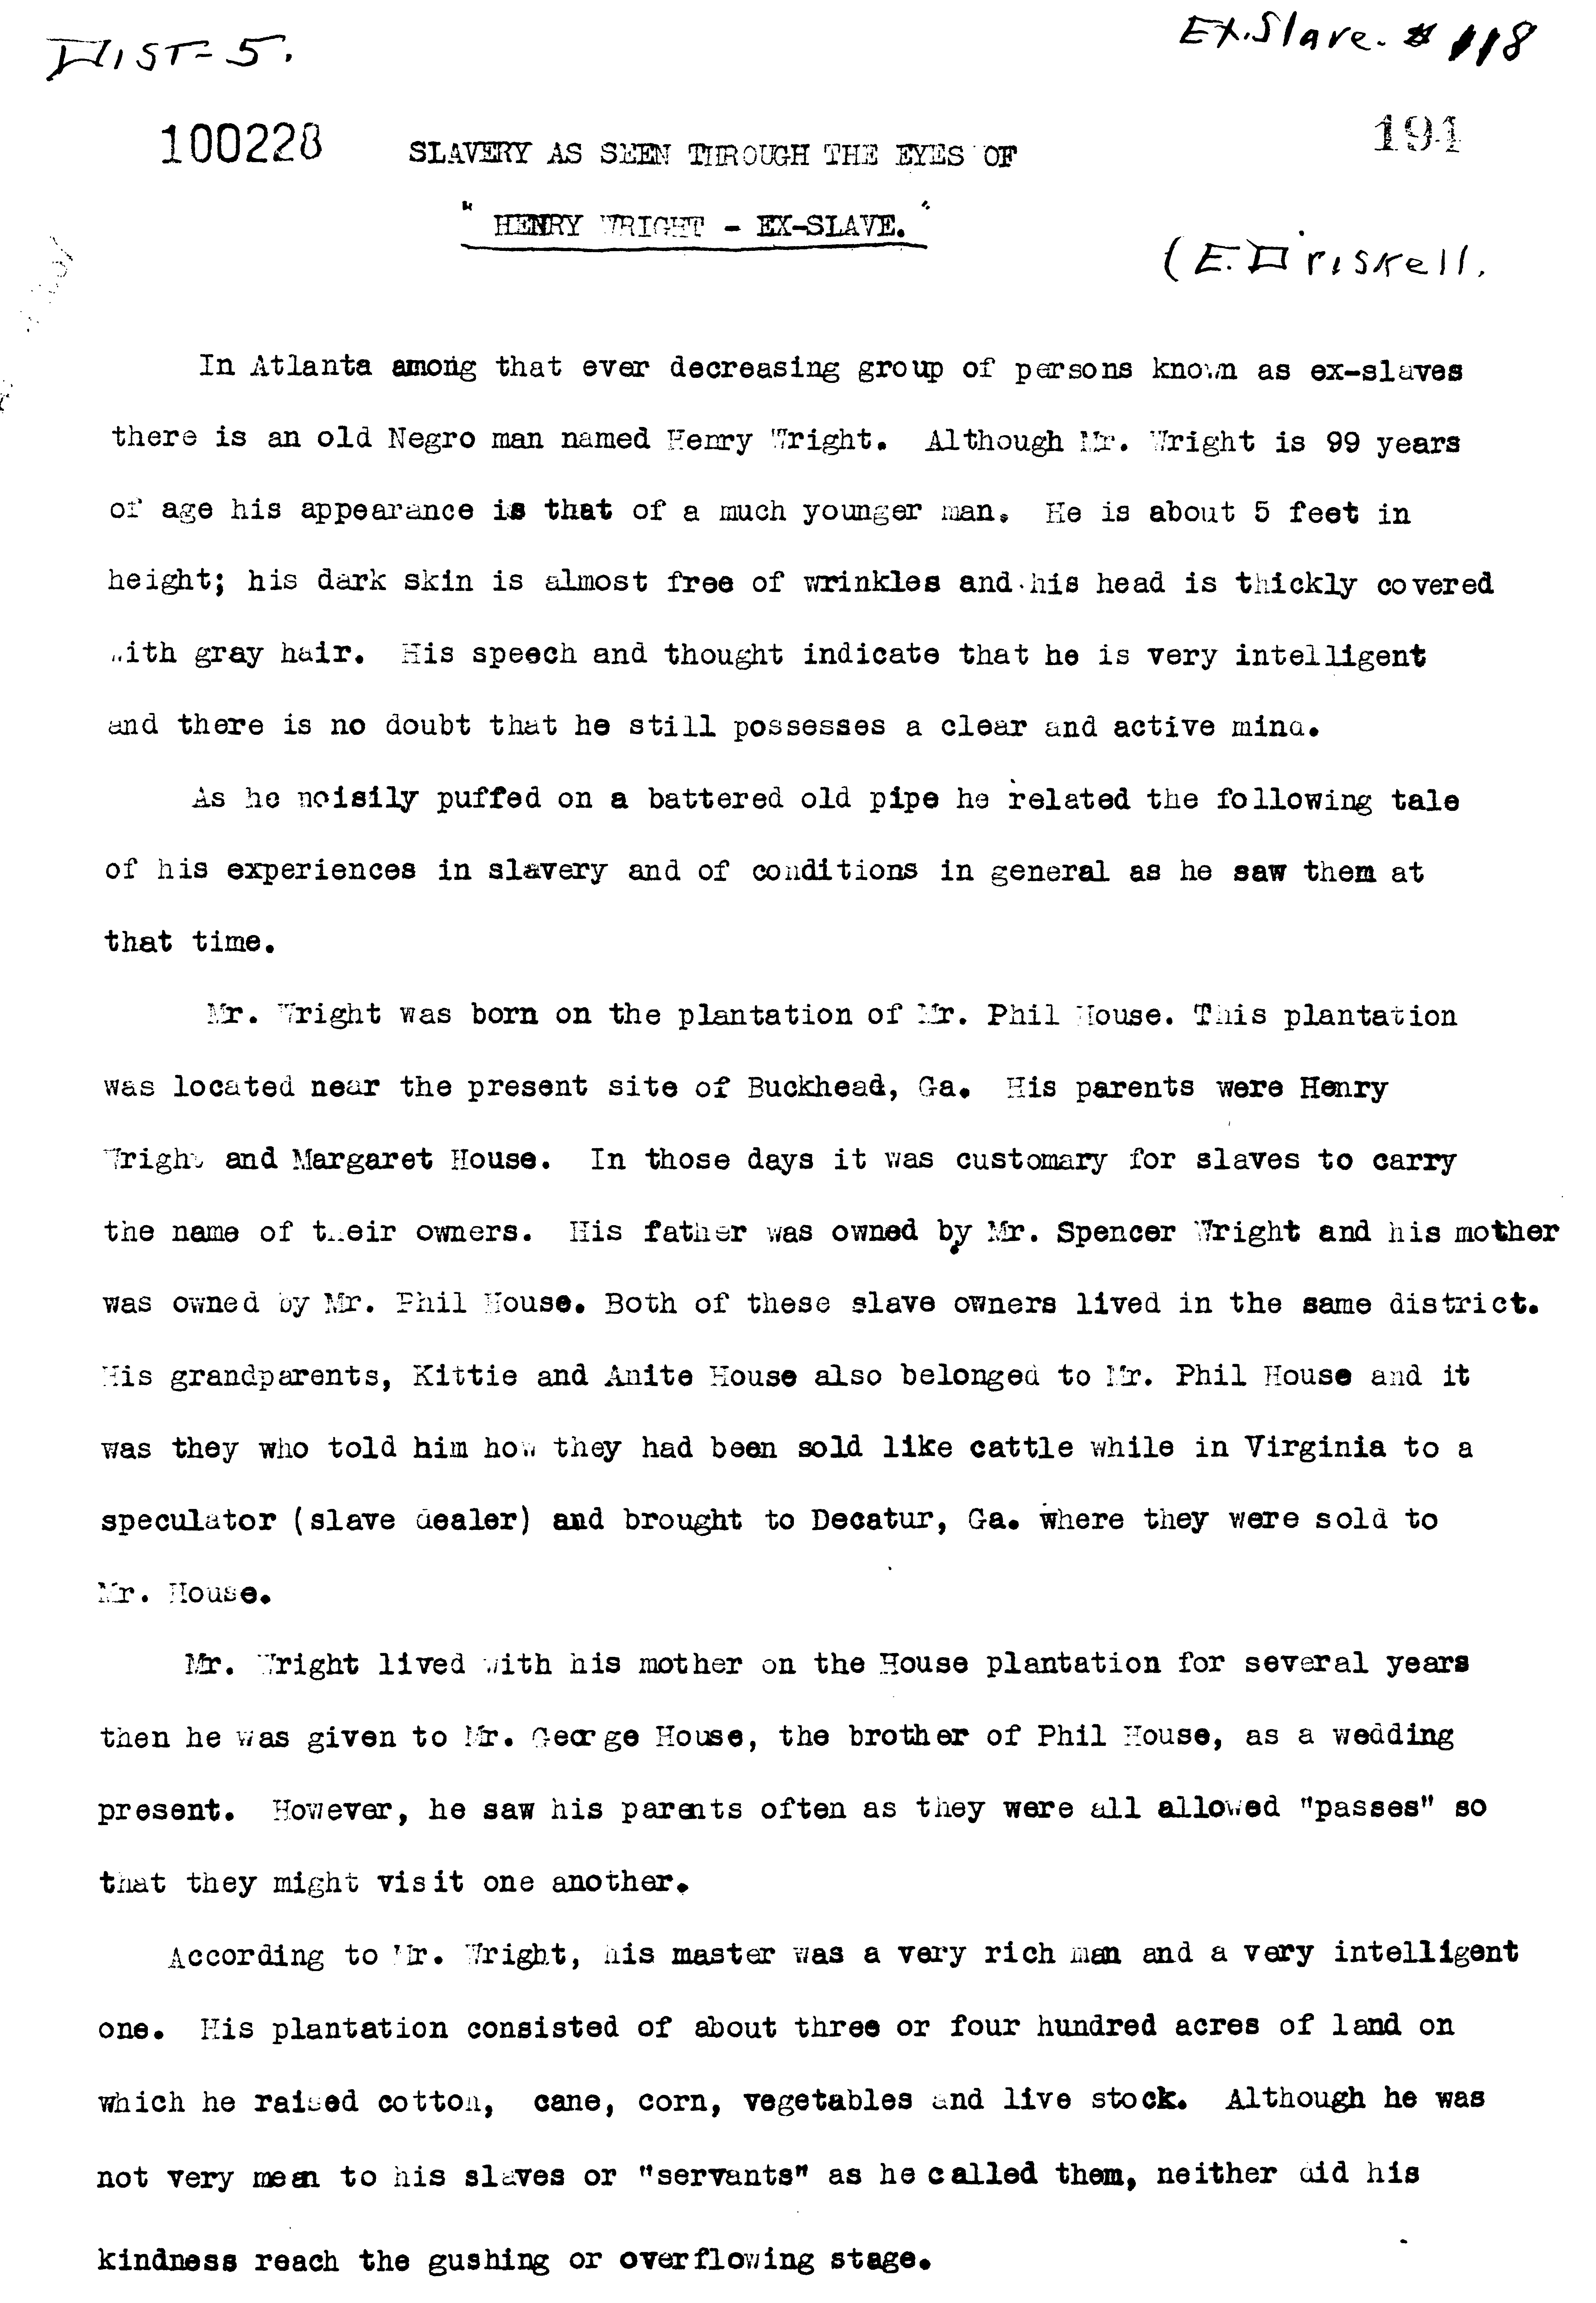
\includegraphics[width=130mm]{./imgs/Cap1.jpg}  
  %\hfill
\end{adjustwidth}
  \caption{Henry Wright, narrativas da Geórgia, Parte \versal{IV}, página 191}
\end{figure}
\end{vplace}

\end{absolutelynopagebreak}

\chapter{Trabalho}
%\addcontentsline{toc}{chapter}{{\large\versal{I.}} Trabalho}
%\hedramarkboth{Trabalho}{}

\subsection{Henry Wright, narrativas da Geórgia, Parte~IV,~páginas~195--97}
\label{ref316}

``Quando jovem, o Sr. Wright precisava coletar lascas pelo pátio,
acender lareiras e buscar água do poço para manter a casa abastecida.
Quando tinha dez anos, foi mandado para o campo, para guiar o arado. Ele
lembra que seus pais também trabalhavam na lavoura. Relatando a sua
experiência como lavrador, o Sr. Wright conta que ele e os outros
escravos eram acordados toda madrugada por um berrante, às três da
manhã. Esse instrumento normalmente era soprado pelo capataz branco ou
pelo capataz negro, conhecido como `capataz negro' entre os escravos. Ao
soar o berrante, eles precisavam se levantar e alimentar o gado. Logo
depois do berrante, um sino era tocado para sinalizar que todos deveriam
partir para a lavoura e começar o dia de trabalho. Eles chegavam à
lavoura antes do sol nascer. O horário de trabalho era descrito como
sendo `de sol a sol'. Quando chegava a colheita do algodão, cada escravo
era obrigado a apanhar pelo menos 90 quilos de algodão por dia. Para tanto,
cada um recebia um embornal e um cesto grande. O saco era pendurado no
pescoço e o cesto era posicionado no fim da linha. No final do dia, o
capataz reunia todos os escravos junto à balança com a lâmpada, a lousa
e a chibata. Qualquer escravo que não apanhasse os 90 quilos obrigatórios
era açoitado severamente pelo capataz. Às vezes, eles conseguiam escapar
desse castigo se davam a desculpa de estarem doentes. Outra estratégia
adotada pelos escravos era umedecer o algodão ou esconder pedras dentro
do cesto, ambos os quais deixavam o algodão mais pesado.

Às vezes, após deixar a lavoura, eles precisavam trabalhar à noite,
debulhando milho, descaroçando algodão ou tecendo. Trabalhava"-se todos
os dias, exceto aos domingos. A única forma de trabalho no domingo era
alimentar o gado, etc. (\ldots{})

As horas de trabalho dos escravos domésticos e os da lavoura eram
praticamente as mesmas. Em alguns casos, os escravos domésticos
precisavam trabalhar à noite, pois o senhor receberia amigos ou fora
convidado a algum lugar, então alguém precisava ficar acordado para
cuidar de todos os detalhes necessários. (\ldots{})

No mau tempo, os escravos não eram obrigados a ir à lavoura, e em vez
disso aparavam a sebe ou faziam outros pequenos serviços em casa. O
senhor não queria que eles trabalhassem em tempo ruim porque havia um
risco grande demais de doença, o que levaria à perda de tempo e de
dinheiro. O Sr. House queria que todos os seus escravos aprendessem um
ofício, como serem pedreiros ou carpinteiros, não porque isso
beneficiaria o escravo, conta o Sr. Wright, mas porque assim ele seria
vendido mais caro caso fosse preciso se desfazer dele. Os escravos que
recebiam permissão para trabalhar com esses artesãos brancos, de quem
aprenderiam o ofício, almejavam a oportunidade, pois teriam permissão
para cobrar por seus serviços. O dinheiro que ganhariam com isso poderia
ser usado para ajudar a comprar a sua liberdade, ou seja, o dinheiro que
sobrava depois que o senhor tomava para si o seu quinhão. O artesão
branco, por outro lado, não tinha nenhuma objeção específica ao fato de
ser auxiliado pelos escravos, apesar de eles estarem aprendendo o seu
ofício, pois podia passar todas as tarefas mais árduas para o escravo, o
que facilitava o seu trabalho''.

\paragraph{Comentário}\quad
{\small
Os escravistas tentavam maximizar a produtividade da sua mão de
obra. Como indica a narrativa de Henry Wright, isso
significava longas horas de trabalho e estratégias para aproveitar as
crianças pequenas e os cativos idosos. Independente da idade, todos os
escravizados tinham trabalho a fazer. Os entrevistados frequentemente
descreviam o seu dia de trabalho como sendo ``de sol a sol'' (ou seja,
do nascer ao pôr do sol) ou ``de consegue a não consegue'' (de conseguir
enxergar até não conseguir mais). Após voltar da lavoura, os homens e as
mulheres muitas vezes tinham tarefas adicionais à noite. Impor esse
trabalho tornava a fazenda mais produtiva e aumentava os lucros, além de
manter os cativos ocupados e afastá"-los do que os donos chamariam de
``encrenca''. Capatazes ou feitores supervisionavam o trabalho no campo
e forçavam a mão de obra a produzir o máximo possível.

Além de trabalhar nas culturas mercantis (algodão em quase todo o
Sul, arroz nas regiões litorâneas da Carolina do Sul e da Geórgia e
açúcar na Luisiana), a maioria dos escravistas tentava produzir a maior
parte da comida necessária para consumo na fazenda. O milho era
cultivado na mesma época que o algodão, da primavera até a colheita no
outono, com os escravizados alternando a sua atenção de uma cultura para a
outra. No outono, quando o milho amadurecia, os trabalhadores muitas vezes
viravam as espigas para baixo para não deixar a chuva encharcá"-las e se
concentravam em apanhar o algodão antes de voltarem para colher o milho.
Criar gado e plantar legumes também podia ajudar a tornar a fazenda
quase autossuficiente e, logo, mais rentável. Em grandes propriedades,
alguns escravizados aprendiam ofícios como, por exemplo, o de ferreiro, para que o
fazendeiro não precisasse pagar pelo trabalho de fora.

Todo o trabalho na lavoura era cansativo. Cultivar e colher
algodão significava longas horas de trabalho sob o sol, muitas vezes
inclinado sobre as plantas. Nos arrozais, os escravizados precisavam
trabalhar com água pelos joelhos nos campos alagados, e o açúcar era uma
cultura especialmente trabalhosa na época da colheita, quando
trabalhavam muitas e muitas horas adicionais, sem dormir, para
ferver o caldo e produzir açúcar e melado.
}

\subsection{Louis Cain, narrativas do Texas, Parte I, páginas 185 e 186} \label{ref42}

``A gente trabalhava enquanto tinha luz, desde as quatro da manhã, e
depois ordenhava as vinte vacas e dava de comer para os bois de canga.
Eram vinte hectares e faltava negro para trabalhar tudo aquilo com
folga\ldots{}

Sábado de manhã, nós homens moíamos milho para o pão da semana e as
mulheres lavavam as roupas do senhor e as nossas. Sábado de noite a
gente dançava até de madrugada, e no domingo os homens saíam para ver as
mulheres ou as namoradas deles enquanto nós os pequenos íamos nadar no
riacho. Todas as noites, menos no sábado, a hora de dormir era nove
horas. O senhor repicava a placa de aço e a gente sabia que estava na
hora de apagar as tochas e se amontoar para dormir''.

\subsection{Simp Campbell, narrativas do Texas, Parte I, páginas 191--92} \label{ref44}

``A fazenda do senhor tinha uns 400 hectares e ele tinha mais de cem
escravos, com um feitor, o Johnson, e um capataz negro. Os negros éramos
bem tratados, mas o feitor tinha ordem de açoitar quem brigasse. Se o
capataz negro chicoteava demais, o feitor vendia ele para outro lugar.

A gente trabalhava das quatro às seis e fazíamos alguma tarefa depois, e
então se sentava e ficava conversando até as nove, quando era hora de ir
para a cama. Sábado de noite, dava para escutar as rabecas e os banjos
tocando e os negros cantando. Os instrumentos todos eram feitos em
casa''.

\subsection{Thomas Cole, narrativas do Texas, páginas 225--29} \label{ref55}

``Eu brincava com os filhos do senhor Cole o tempo todo, e quando fiquei
mais velho ele me pôs a trabalhar buscando madeira e outros servicinhos
assim, e também dando de comer para os porcos. Os pequenos tinham que
apanhar algodão todo outono. Os cestões pesavam uns 35 a 45 quilos, mas
nós pequenos botávamos o nosso no cesto de um escravo adulto. Os
escravos adultos eram que nem mulas. Eles trabalhavam para ter o que
comer e o que vestir, e tinha uns que sofriam mais que as mulas, porque
as mulas comiam bem e os escravos às vezes passavam fome. Mas o senhor
Cole era um homem esperto e bom com essas coisas. Ele tinha respeito
pelos sentimentos dos escravos e não tratava eles feito uns bichos
estúpidos, os escravos dele tinham mais privilégios do que o de qualquer
outro senhor por aquelas partes. Ele foi um dos melhores homens que já
vi em toda a minha vida e a mulher dele era igualzinha. (\ldots{}) A
gente acordava cedo todos os dias do ano, fizesse chuva ou fizesse sol,
frio ou calor. Um escravo soprava o berrante e não tinha perigo de você
não acordar com aquele barulho alto e comprido como era. Ele subia numa
plataforma duns três metros para soprar aquela corneta. A gente
trabalhava até o meio"-dia, então comia na sombra e descansava uma hora,
um pouquinho mais quando estava quente, mas só uma hora quando estava
frio. Você fica sempre cansado quando o dia é assim na fazenda, não dá
para se divertir a noite inteira que nem os jovens fazem hoje em dia.
Mas a gente tinha sorte, porque o senhor Cole não nos castigava. O homem
nosso vizinho, ele castigava muito os escravos dele, muito mesmo.
(\ldots{}) {[}Depois que o seu senhor morreu{]} Eu pensei comigo mesmo,
aquele Sr. Anderson, o feitor, ele vai me lanhar com o bacalhau
{[}\emph{cat-o'-nine-tails}{]} na primeira chance que tiver, mas decidi que ele
não ia ter chance nenhuma, pois eu ia fugir na primeira chance que
tivesse. Eu não sabia como ia fugir de lá, mas ia para o Norte, onde não
tem senhor de escravos. (\ldots{}) Estavam falando de guerra e a gente
estava indo para o eito mais cedo e ficando até mais tarde. Milho levado
embora, algodão levado embora, porcos e gado arrebanhados e levados, a
coisa ia ficar ruim. A guerra começou, mas a gente não viu nada dela. Só
que em vez de comer pão de milho, a gente comia pão de milho"-zaburro. A
gente plantou bastante quiabo e disseram que ele ia ser tostado e moído
para fazer café para os brancos. Isso também não parecia muito bom.
Naquele inverno, em vez de abater 300 ou 400 porcos, como a gente sempre
fez antes, abatemos só 175, e nem foram todos os grandões. Quando o
estoque de carne começava a acabar, o Sr. Sandson mandava uns escravos
caçarem um veado ou porcos selvagens ou o que desse para achar''.

\subsection{Elisabeth Sparks, narrativas da Virgínia, página 51}
\label{ref249} 

``Eles trabalhavam seis dias, de sol a sol. Se era a colheita de trigo ou
outra safra, o trabalho começava bem antes do dia nascer. O dia de
trabalho normal começava quando o berrante soprava. Eles paravam só o
bastante para comer ao meio"-dia. Não tinha muita comida. Eles ganhavam
um pouco de sebo e uma fatia de pão de manhã. Bem, eles davam uma ração
para os negros toda semana. O almoço era uma fogaça assada em cima de
uma enxada''.

\subsection{Emma Hurley, narrativas da Geórgia, Parte II, página 276}
\label{ref157}

``O trabalho dos escravos na fazenda era difícil. As mulheres
trabalhavam o dia inteiro no eito e depois fiavam de noite. Cada uma
tinha que fiar seis fusos por semana. No sábado, uma `senhora branca'
desenrolava a fiação e se uma das mulheres não tinha feito a sua tarefa,
ela apanhava feio. Os homens trabalhavam o dia inteiro e ficavam até as
dez da noite debulhando milho ou em outras lidas à luz do lampião''.

\subsection{Sallie Carder, narrativas do Oklahoma, páginas 27--28} \label{ref47}

``Lá pelas quatro da manhã, o feitor ou o cocheiro negro que ficava na
casa grande tocava o sino para a gente levantar e ir trabalhar. Os
escravos apanhavam uma pilha de algodão e trabalhavam até tarde nas
noites de luar''.

\subsection{Frances Willingham, narrativas da Geórgia, Parte~IV,~página~156}
\label{ref295}

``Nosso feitor juntava todos os escravos antes do dia nascer e eles
tinham que já ter comido o desjejum e chegado no campo quando o sol
aparecesse. O sol estava mais que posto quando eles chegavam em casa de
noite''.

\subsection{William McWhorter, narrativas da Geórgia, Parte~III,~páginas~98--99}
\label{ref188}

``Quando o assunto era trabalho, nunca se tinha folga nenhuma. Quando os
escravos voltavam do eito depois do pôr do sol e cuidavam do gado e da
janta, os homens ainda tinham que debulhar milho, consertar canga de
cavalo, cortar madeira e coisas assim; as mulheres costuravam, fiavam,
teciam e algumas tinham que ir para a casa grande e dar de mamar para os
bebês dos brancos. Uma noite, minha mãe tinha dado de mamar para um dos
bebês brancos e depois que ele pegou no sono, ela foi colocar ele na
caminha. O pé da criança se prendeu nos suspensórios do senhor Joe, que
ele tinha pendurado no pé da cama, e quando ele escutou o bebezinho
chorando o senhor Joe acordou, agarrou um pedaço de pau e bateu na
cabeça da minha mãe até que quase matou ela. Minha mãe nunca ficou bem
de verdade depois disso, e quando morreu ainda tinha um calombo enorme
na cabeça.

Dizem que em algumas fazendas os escravos ficavam liberados quando o
sino do almoço tocava no domingo, mas não na nossa. Lá não tinha
descanso até o sol se pôr nas noites de domingo, depois que tinham
cuidado do gado e comido a janta. Nos domingos, eles podiam fazer umas
visitas depois da igreja, mas ainda tinham que tomar cuidado e levar um
passe. O senhor Joe dava um dia para os escravos fazerem o seu Natal.''

\subsection{John W. Fields, narrativas do Indiana, página 78} \label{ref89}

``Minha vida antes dessa época {[}quando minha mãe recebeu permissão
para visitar{]} foi repleta de tristeza e desespero. Nós acordávamos
entre quatro e cinco da manhã, e pais e filhos trabalhavam arduamente
até o cair da noite nos dar trégua. Depois de um jantar minguado,
geralmente conversávamos até ficar com sono e ter que ir para a cama. Os
que tinham a sorte de saber, liam''.

\subsection{Yach Stringfellow, narrativas do Texas, Parte~\versal{IV},~página~68}
\label{ref254} 

``Nós escravos usávamos tochas de pinho, às vezes uns tocos de vela. As
mulheres faziam todas as velas dos brancos elas mesmas. A gente não
precisava de muita luz à noite de tão cansados depois do dia comprido
trabalhando de consegue a não consegue enxergar, e ia para cama cedo.
(\ldots{})

O senhor botou o John de feitor, e ele era um marchador. Ele estava em
tudo quanto é lugar onde ninguém achava que ele ia ir. Ele tinha um
vozeirão e todos nós cantando e chorando `Olha bem, negro, olha bem, lá
vem encrenca'. Se um negro ou uma negra tinha deitado no milharal, eles
se levantavam rapidinho e se ocupavam na hora, porque aquele chicote
corria atrás deles. Eles se ajeitavam e viravam os mais esforçados da
turma quando o John chegava''.

\subsection{Sarah Gudger, narrativas da Carolina do Norte, Parte~I,~página~353}
\label{ref114}

``Não, senhora, eu nunca soube o que era descansar. Eu só trabalhava o
tempo todo, da manhã até o fim da noite. Eu tinha que fazer de tudo fora
de casa. Trabalhar no eito, cortar madeira, capinar talos, até que às
vezes minhas costas pareciam que iam quebrar. Eu fazia de tudo, menos
rachar toras. Sabe como é, eles rachavam toras naquela época, mas eu
não, eu nunca rachei tora nenhuma.

O velho senhor nos dava uma tunda se a gente fazia alguma coisa que ele
não gostava. Às vezes ele ficava fulo, e nessas horas a gente nem olhava
para ele. Se não, ele amarrava as nossas mãos na frente do corpo e
chicoteava que nem se faz com uma mula. Meu Deus, eu levei mil
chibatadas quando era nova. Às vezes, meu pobre corpo doía uma semana
inteira.

O velho senhor nos mandava trabalhar em tudo que era tempo, na chuva e
na neve, nunca fazia diferença. A gente precisava ir até as montanhas,
derrubar árvores e arrastar elas de volta para casa. Muitas e muitas
vezes a gente voltava com as roupas grudadas nos nossos corpos gelados,
mas não adiantava nada tentar deixar elas secas. Se o velho senhor ou a
senhora nos viam, eles gritavam: `Sai daqui, coisa preta, e vai
trabalhar de uma vez!' Meu Deus, e a gente saía correndo mesmo. Se não,
lá vinha o chicote''.

\subsection{Fred Brown, narrativas do Texas, Parte I, páginas 156--57} \label{ref35}

``O senhor tinha uma fazenda muito bonitinha na Luisiana, neste lado do
rio Mississippi. De escravos, ele chegava a ter de 40 a 50. Na nossa
família tinha papai, mamãe, três irmãos e uma irmã, a Julia, e seis
primos. Isso dá 13, é por isso que o senhor se incomodava tantos com
negros fujões.

\textls[-10]{Todo mundo lá tinha certos trabalhos e deveres para fazer. Mamãe era a
cozinheira da família e ajudava no tear, fazendo o tecido. Meu papai era
o ferreiro, o sapateiro e o curtidor. Vou explicar como era o curtume.
Ele colocava o couro na água com casca de carvalho"-negro e logo, logo o
pelo caía, e depois ele enrolava e martelava o couro para deixar ele
macio.}

Quando eu tinha uns oito anos, mais ou menos, eles me botaram para
ajudar no pátio. Depois que cresci, comecei a ajudar no eito. O senhor
plantava quase só cana e milho, nada de algodão''.

%\pagebreak
\begin{figure}[]
%\thisfloatpagestyle{empty}
%\begin{minipage}{0,4\textwidth}
\centering
 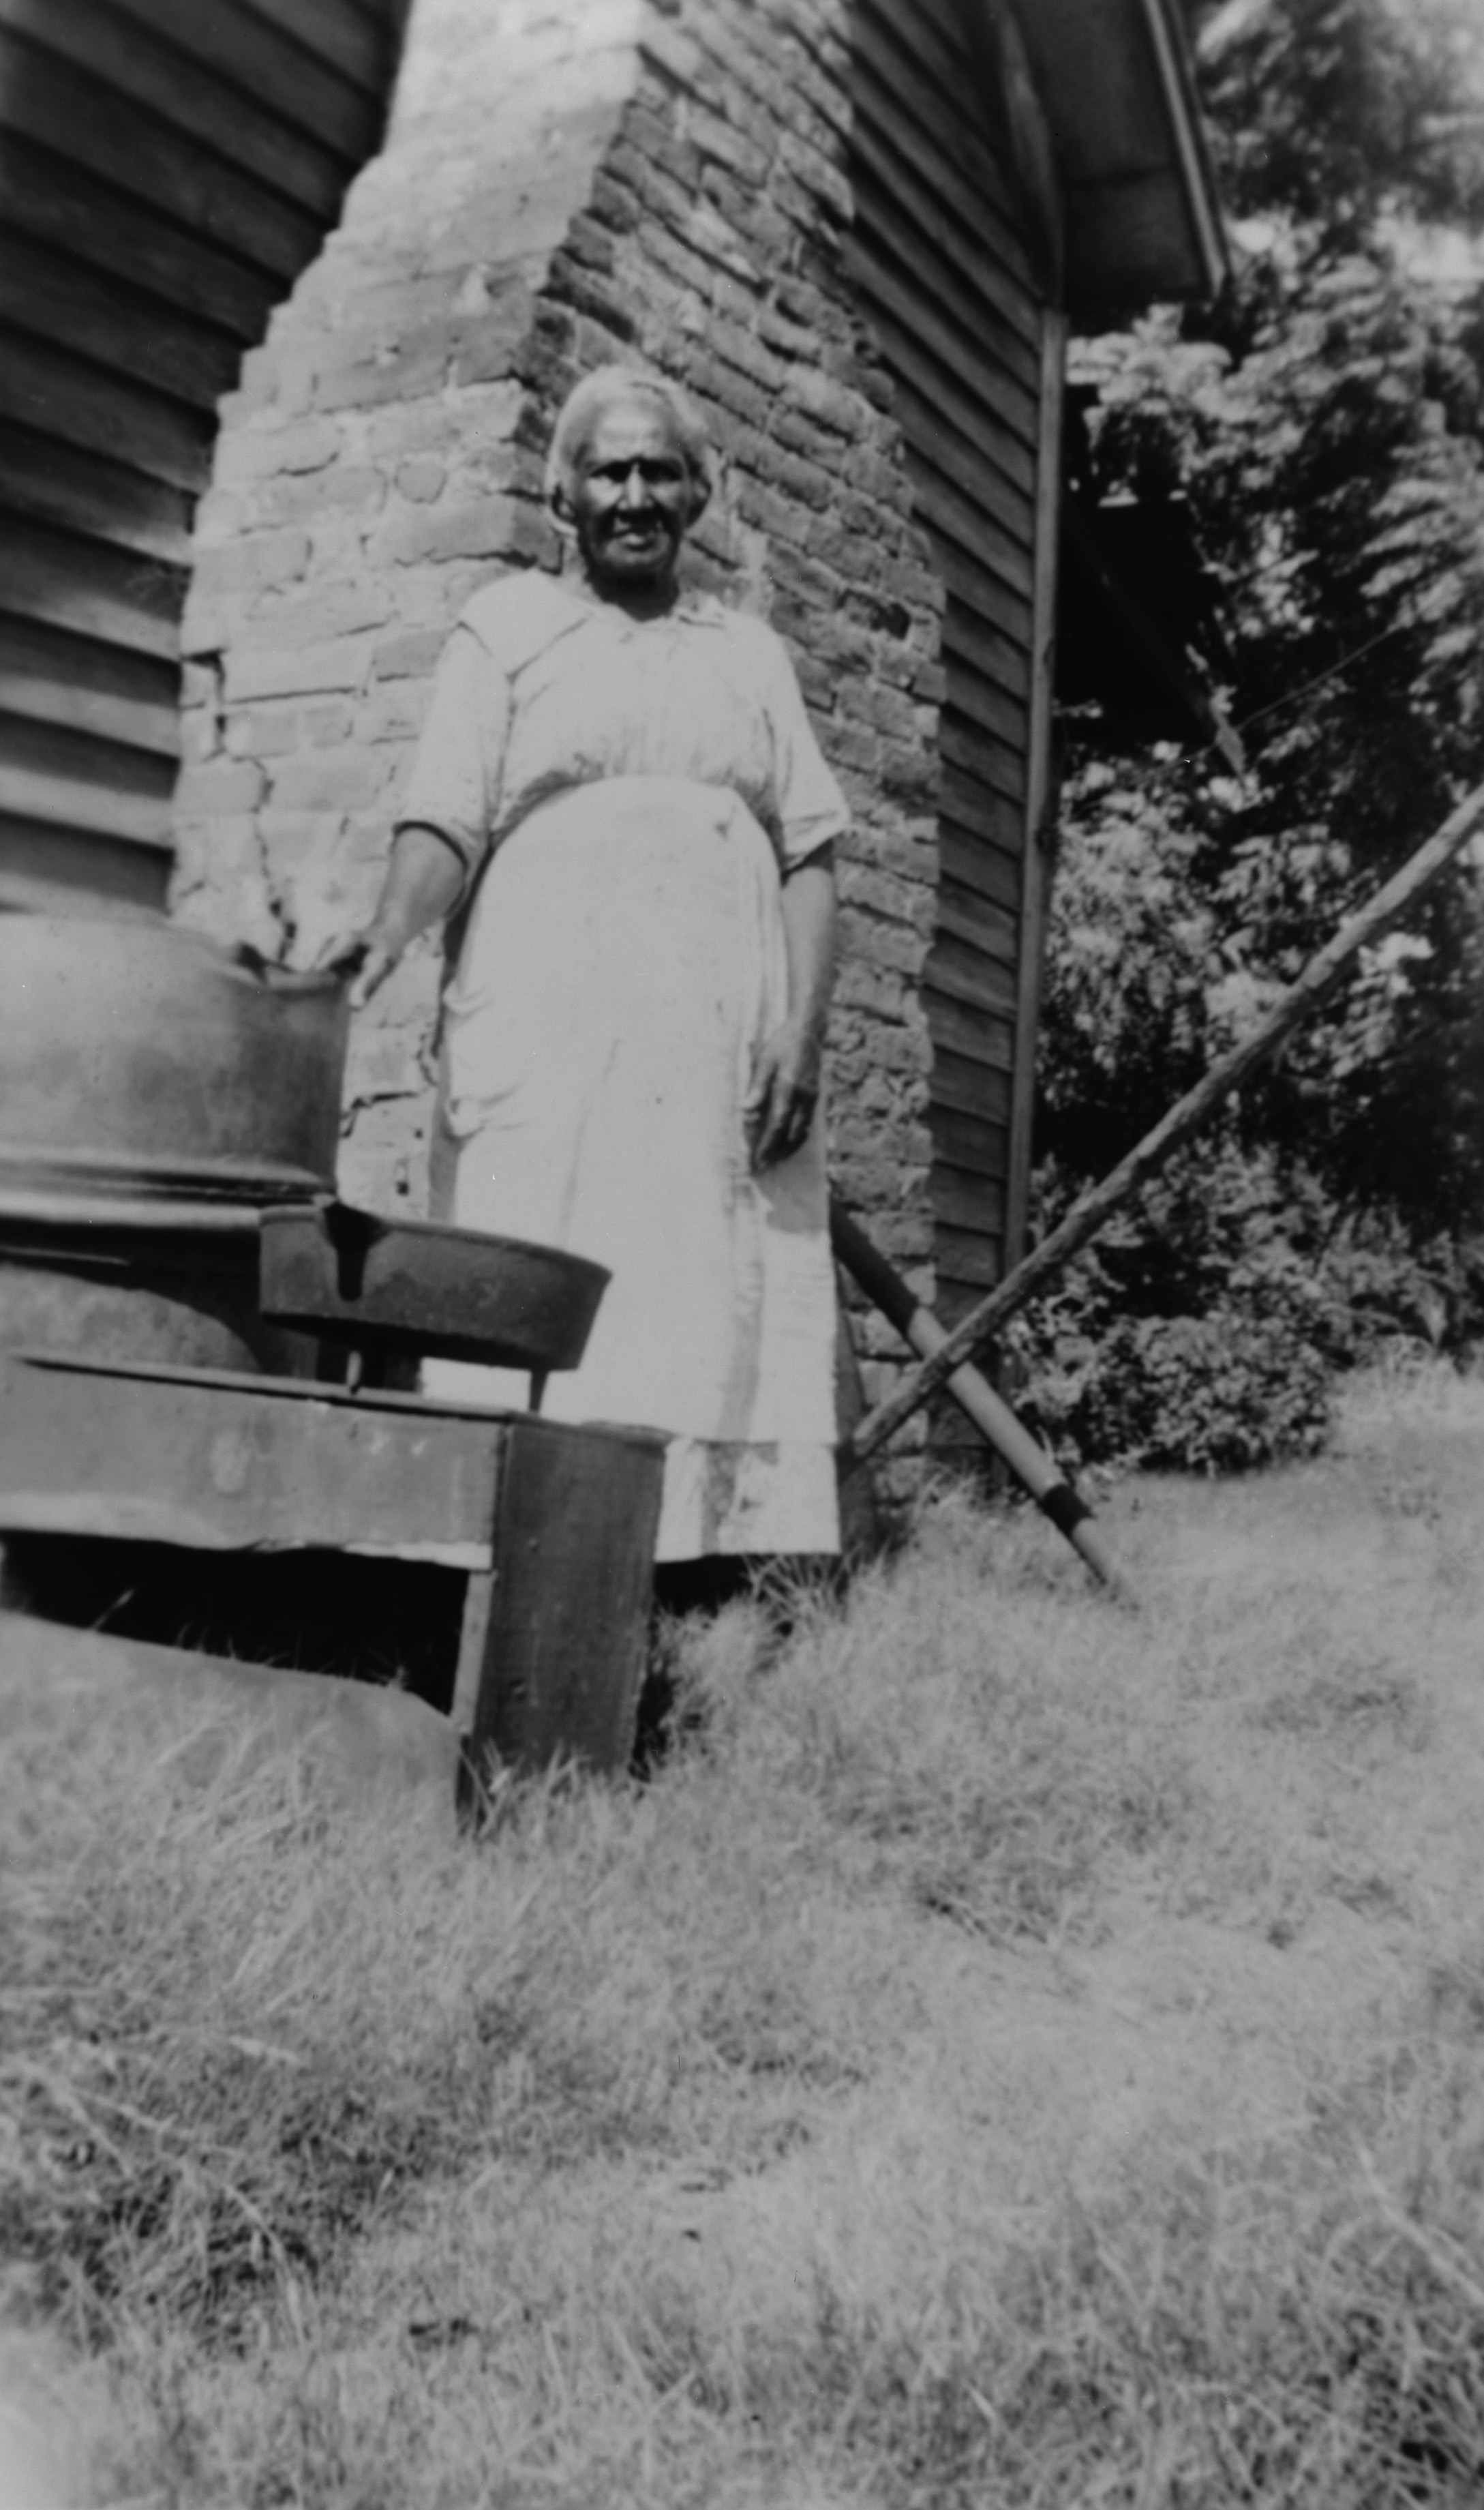
\includegraphics[width=90mm]{./imgs/katiedarling_recorte.jpg} \label{img1}
\caption{Katie Darling}
%\end{minipage}
\end{figure}


\subsection{Katie Darling, narrativas do Texas, Parte~I,~páginas~278--79} \label{ref65}

``Você está falando com uma negra que deu de mamar para sete branquinhos
nos tempos do relho. (\ldots{}) Eu e meus três irmãos, Peter e Adam e
Willis, todos sobrevivemos, crescemos e casamos, mas mamãe morreu na
escravidão e papai fugiu quando ele e o senhor Bill estavam a caminho da
Batalha de Mansfield.\footnote{Batalha travada na Luisiana em 8 de abril de 1864,
durante a Guerra Civil norte"-americana.} Quando voltou da guerra, o senhor disse: `Aquele
crioulo imprestável fugiu e se juntou com aqueles yankees duma figa'.

O senhor tinha seis filhos quando a guerra começou e eu dei de mamar
para todos eles. Eu ficava em casa com eles e dormia em um catre no
chão, e assim que cresci o suficiente para carregar o balde de leite,
eles me botaram na ordenha também. O senhor tinha mais de 100 vacas, e
quase sempre quem ordenhava todas elas éramos nós duas, Violet e eu. A
gente tinha que estar no curral às cinco. Teve uma manhã que o senhor me
pegou deixando um dos bezerros mamar e ele não me castigou daquela vez,
mas isso não quer dizer que ele era sempre bonzinho, porque as vacas
tinham mais coração que o senhor e a senhora.

Nós comíamos ervilha, verdura, couve e sêmea. Os negros que mexessem no
presunto! A gente ganhava café de farinha de milho. A farinha era
tostada no fogão e fervida e a gente tomava o licor. Às vezes, a gente
ganhava o café Lincoln que sobrava da fazenda vizinha.

Quando os negros faziam qualquer coisa, o senhor dava relhadas nele, mas
de arrancar a pele era pouco. Ele castigava o homem por arar ou capinar
pela metade, mas se faziam o serviço direito ele achava outro motivo
para puxar a chibata. À noite, os homens tinham que debulhar milho e as
mulheres cardavam e fiavam. A gente tinha duas mudas de roupa para o
inverno e duas para o verão, mas nada de sapato. A gente trabalhava
sábado o dia inteiro, e se tinha erva no campo, ninguém ganhava o
domingo de folga''.

\subsection{Wes Brady, narrativas do Texas, Parte I, página 135} \label{ref31}

``O meu primeiro serviço foi plantando milho, depois no curral com as
vacas e de pastor das ovelhas. Todos nós da casa tínhamos que descascar
meio alqueire de milho todas as noites para dar de comer para as
ovelhas. Várias vezes eu fiquei caminhando pela senzala quando era
pequenino, chorando e chamando minha mãe. A gente quase só se via no
domingo. As crianças estavam na cama quando os outros saíam para o campo
e quando voltavam. Lembro de acordar de noite várias vezes e ver eles
fazendo mingau nas brasas da lareira, mas ela sempre garantia que o
feitor estava dormindo antes''.

\subsection{George Womble, narrativas da Geórgia, Parte~\versal{IV},~páginas~181--83}
\label{ref306}

``Nenhum deles nunca sofreu daquela doença, a `febre do colchão'. Todos
levantavam muito antes do dia nascer e preparavam o desjejum e antes de
ficar claro o suficiente para enxergar, eles já estavam de pé no eito,
com as enxadas e os outros implementos, com medo de começar a trabalhar.
Eles não queriam sujar os algodoeiros de terra naquela escuridão.

Em dias de chuva, os escravos debulhavam milho, amontoavam esterco nos
celeiros e faziam tecido. No inverno, os homens rachavam toras,
construíam cercas e escavavam valas, enquanto as mulheres fiavam e
teciam. Os escravos idosos demais para trabalhar na lavoura ficavam em
casa, onde cuidavam dos escravos doentes (quando havia doença) e das
necessidades das crianças pequenas demais para trabalharem na lavoura.
As crianças que ainda não haviam sido desmamadas também ficavam sob o
cuidado dessas pessoas idosas. Contudo, nesse caso, as mães tinham
permissão para sair da lavoura duas vezes ao dia (uma vez entre o
desjejum e o almoço, outra entre o almoço e o jantar) para que essas
crianças pudessem ser alimentadas''.

\subsection{John Walton, narrativas do Texas, Parte \versal{IV}, página 125}
\label{ref273}

``Eu trabalhei no campo naqueles lados, e até nós, as crianças, tínhamos
que apanhar 70 quilos de algodão por dia, ou lá vinha uma tunda. A gente
botava o algodão nos cestos de carvalho branco, e em alguns deles cabia
quase 50 quilos. Tudo depende de como você prensa o algodão. A carroça
com a parelha de bois ficava no campo, esperando para a gente despejar o
algodão, e quando ela se enchia os bois puxavam a carroça até o
descaroçador movido a cavalo. Normalmente a gente usava cerca de 725
quilos de algodão para cada fardo''.

\paragraph{Comentário}\quad
{\small
Os entrevistados não se lembravam do trabalho árduo apenas porque
este era cansativo. Ele também envolvia pressão, o medo de castigos
físicos e muitos desconfortos, privações e lesões. Como os proprietários
tentavam mantê"-los ocupados quase todo o tempo, os escravizados também se
ressentiam do confinamento e da falta de oportunidade de ir e vir. A
mobilidade era realmente importante para os cativos das fazendas
menores, pois desejavam ter contato social com camaradas ou
parentes em fazendas vizinhas. Essa questão é bastante relevante, pois
apenas metade da população escrava dos Estados Unidos morava em
fazendas com 20 cativos ou mais, de acordo com os dados disponíveis
para 1860. Assim, a outra metade dividia sua rotina diária com apenas
três ou quatro outras famílias afro"-americanas. Entre os escravistas
brancos, 88\% tinham menos de 20 cativos, e 72\% tinham menos de dez.
}


\subsection{Mary Reynolds, narrativas do Texas, Parte~\versal{III},~páginas~238--40,~242}
\label{ref222}

``O senhor Kilpatrick não era nenhum pobretão. Ele tinha riquezas. Tinha
uma casa grande, sem mais estilo que um berço, mas dava para morar
bastante gente lá. Ele era um doutor de medicina e no segundo andar
tinha quartos para os doentes que vinham descansar. Demorava dois dias
para cruzar todas as terras dele. Ele tinha gado e bichos e ovelhas e
mais de cem escravos, e não só isso. (\ldots{})

Ele plantava milho, algodão, cana, batata e amendoim, e também ervilha e
outras comidas para os negros. Lembro de segurar o cabo de uma enxada,
tremendo todo, quando botaram uma velha para me ensinar e umas outras
crianças para capinar o eito. Aquela velha corria feito maluca. Ela me
mostrava o que fazer, depois virava para mostrar para algum outro
negrinho, e então eu cortava o milho novo bem cortadinho. E ela dizia
`Pelo amor de Deus, melhor aprender direitinho, ou o Solomon vai te
espancar até não poder mais'. O velho Solomon era o capataz negro.
(\ldots{})

A concha soprava logo antes do sol raiar e todos tinham que sair
correndo para a chamada, ou então o Solomon derrubava a porta para
buscar eles. O trabalho era difícil, com surras e pouca comida. Uma mula
velha puxava uma tábua com a água e as comidas. Várias vezes tinha só
meio barril de água, velha e quente, para todos os negros nos dias mais
quentes. O que mais se comia era porco defumado, pão de milho, ervilha,
feijão e batata, mas nunca tinha tudo que a gente precisava.

As épocas que eu mais odiava eram as de apanhar algodão com gelo nos
capulhos. Minhas mãos doíam e se rachavam e sangravam. A gente acendia
uma fogueira no campo e quando quem tinha as mãos doloridas não
aguentava mais, a gente corria para esquentar as mãos um pouquinho.
Quando conseguia roubar uma batata, eu costumava colocá"-la no meio das
cinzas, então quando corria para a fogueira eu tirava ela de lá e comia
escondida.

Às vezes, o senhor deixava os negros terem uma hortinha. Eles
plantavam batata e amendoim. Eles gostavam disso, dava para aumentar o
sustento. Batata assada nas cinzas era a coisa mais gostosa que eu
comia. Eu morria de satisfeita só de ter mais uma batata assada nas
brasas. Os negros tinham que trabalhar na roça e escavar as batatas e os
amendoins de noite. Depois, se queriam vender elas na cidade, tinham que
pedir um passe para irem. Eles tinham que ir à noite, porque nunca
deixavam faltar ninguém no eito.

De vez em quando, nos davam um pouco da noite de sábado para lavar as
nossas roupas no rio. A gente estendia elas no chão da floresta para
secar. Tinha um lugar para lavar as roupas com a água do poço, mas tinha
tantos negros que nem todo mundo conseguia lavar no domingo. (\ldots{})


Tinha uma cabana que chamavam de casa de fiar, com dois teares e duas
rodas de fiar funcionando o tempo inteiro e duas negras costurando o
tempo inteiro. Uma fazenda daquele tamanho precisava de muita costura
para fazer tudo que gastava. Uma vez, o senhor foi a Baton Rouge e
trouxe de volta uma moça mulata vestida toda elegante. Era uma negra
costureira. Ele construiu uma casa para ela longe da senzala e ela fazia
a costura fina para os brancos. Os negros sabiam que o doutor pegava uma
negra como pegava uma branca e pegava quem bem entendia nas suas terras,
e pegava bastante. Mas quase todas as crianças que nasciam por lá
pareciam negras. Tia Cheyney sempre disse que quatro dos dela eram do
senhor, mas ele não dava bola para eles''.

\begin{figure}[]
%\begin{minipage}{0,4\textwidth}
\centering
 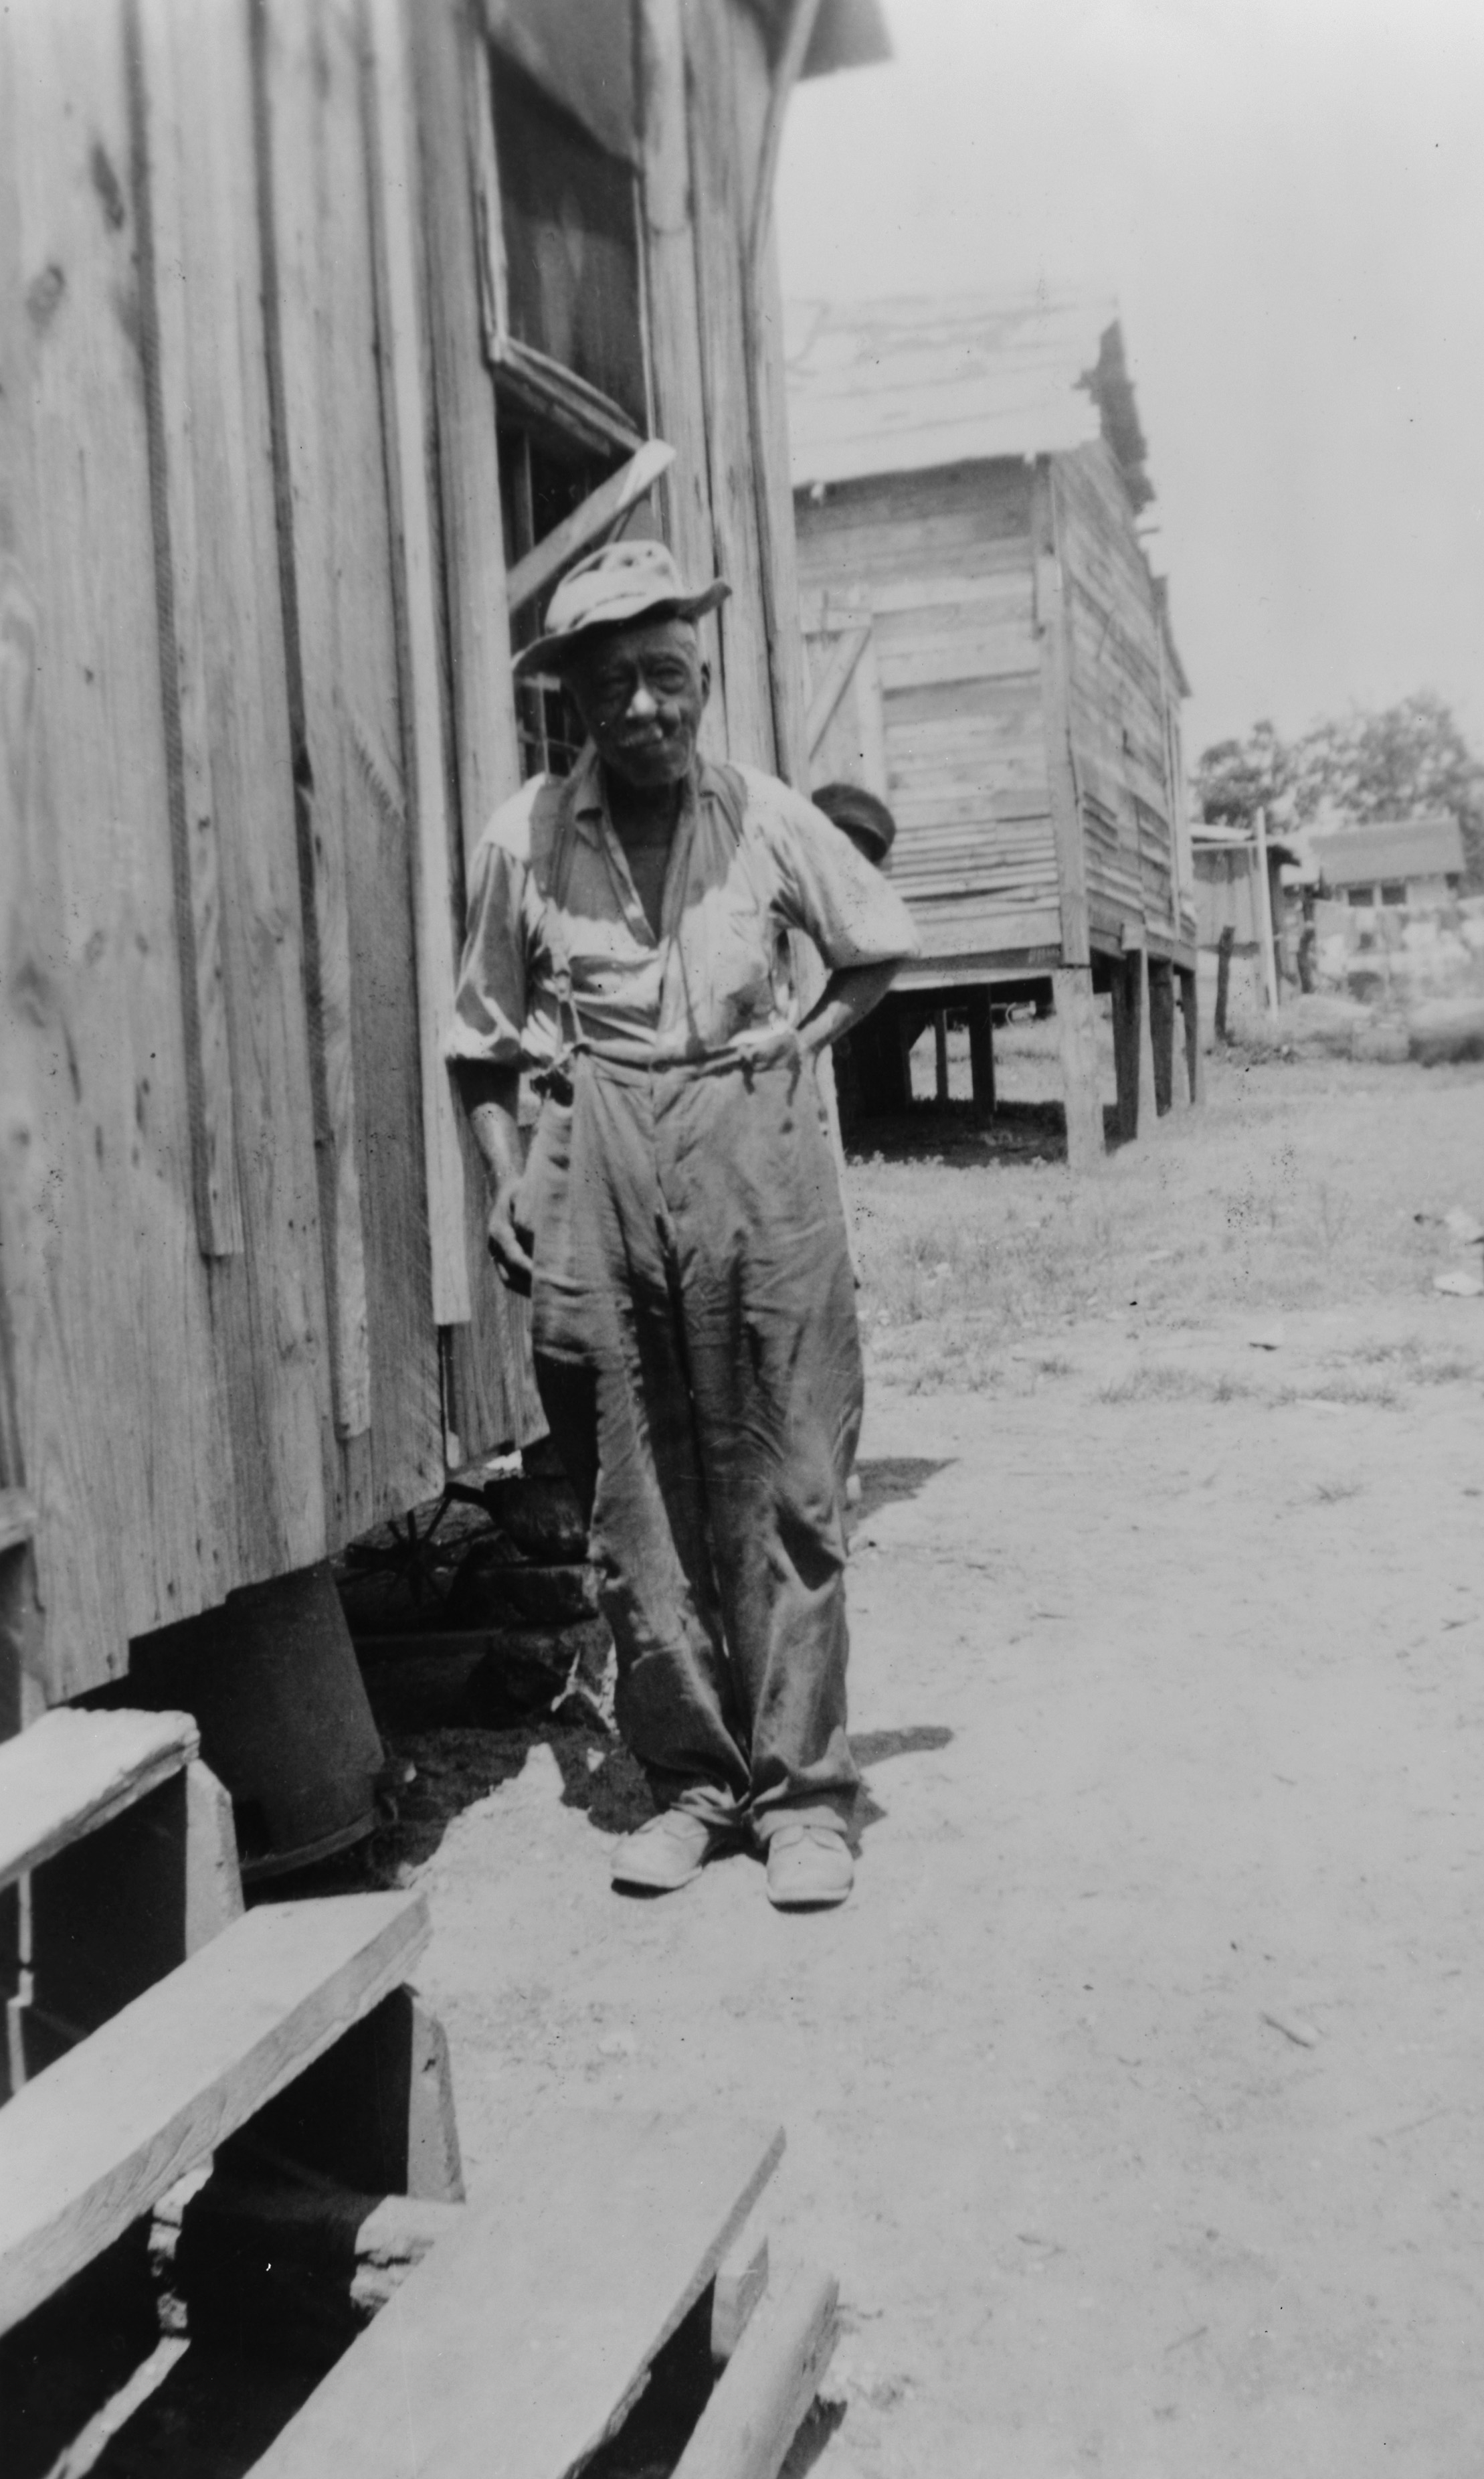
\includegraphics[width=90mm]{./imgs/jordonsmith_recorte.jpg} \label{img2}
\caption{Jordon Smith}
%\end{minipage}
\end{figure}

\subsection{Jordon Smith, narrativas do Texas, Parte \versal{IV}, página 37}
\label{ref244}

``O senhor Ab tinha centenas de hectares de trigo e fazia as mulheres
empilharem feno no campo. Às vezes, elas ficavam doentes e queriam ir
para casa, mas ele mandava elas deitarem em uma pilha de palha no meio
do campo. Várias crianças nasceram na palha do campo. Depois que a
criança nascia, ele mandava elas para a casa. Eu vi com os meus próprios
olhos''.

\subsection{Wash Ford, narrativas do Arkansas, Parte \versal{II}, página 326} \label{ref92}

``Tem uma história que eu lembro dos meus pais. Eles tinham um líder que
capinava algodão. O nome dele era John. Ele trabalhava rápido. John
capinava uma linha e então se esticava para capinar a outra. Ele se
adiantava muito na frente dos outros, que levavam uma sova se não
acompanhassem, então ele descansava para eles alcançarem''.

\subsection{Isaac Green, narrativas da Geórgia, Parte \versal{II}, página 58}
\label{ref112}

``Todos os escravos tinham que trabalhar. Minha mãe trabalhava no arado.
Todos os velhos e as velhas tinham que cuidar dos porcos e das vacas e
também fiar e costurar. Às vezes, o velho senhor nos deixava fazer um
festejo e a gente podia dançar a noite toda se quisesse, desde que
estivesse pronto para ir para o eito quando o feitor soprasse a corneta
antes da manhã seguinte. Os trabalhadores acordavam cedo o suficiente
para fazer o desjejum antes de irem para o eito. As crianças levavam o
almoço para eles ao meio"-dia. A gente usava cestos para levar o almoço e
uns baldes enormes para levar o leite. Eles tinham que fazer a própria
janta quando saíam do campo de noite''.



\begin{figure}[]
%\begin{minipage}{0,4\textwidth}
\centering
 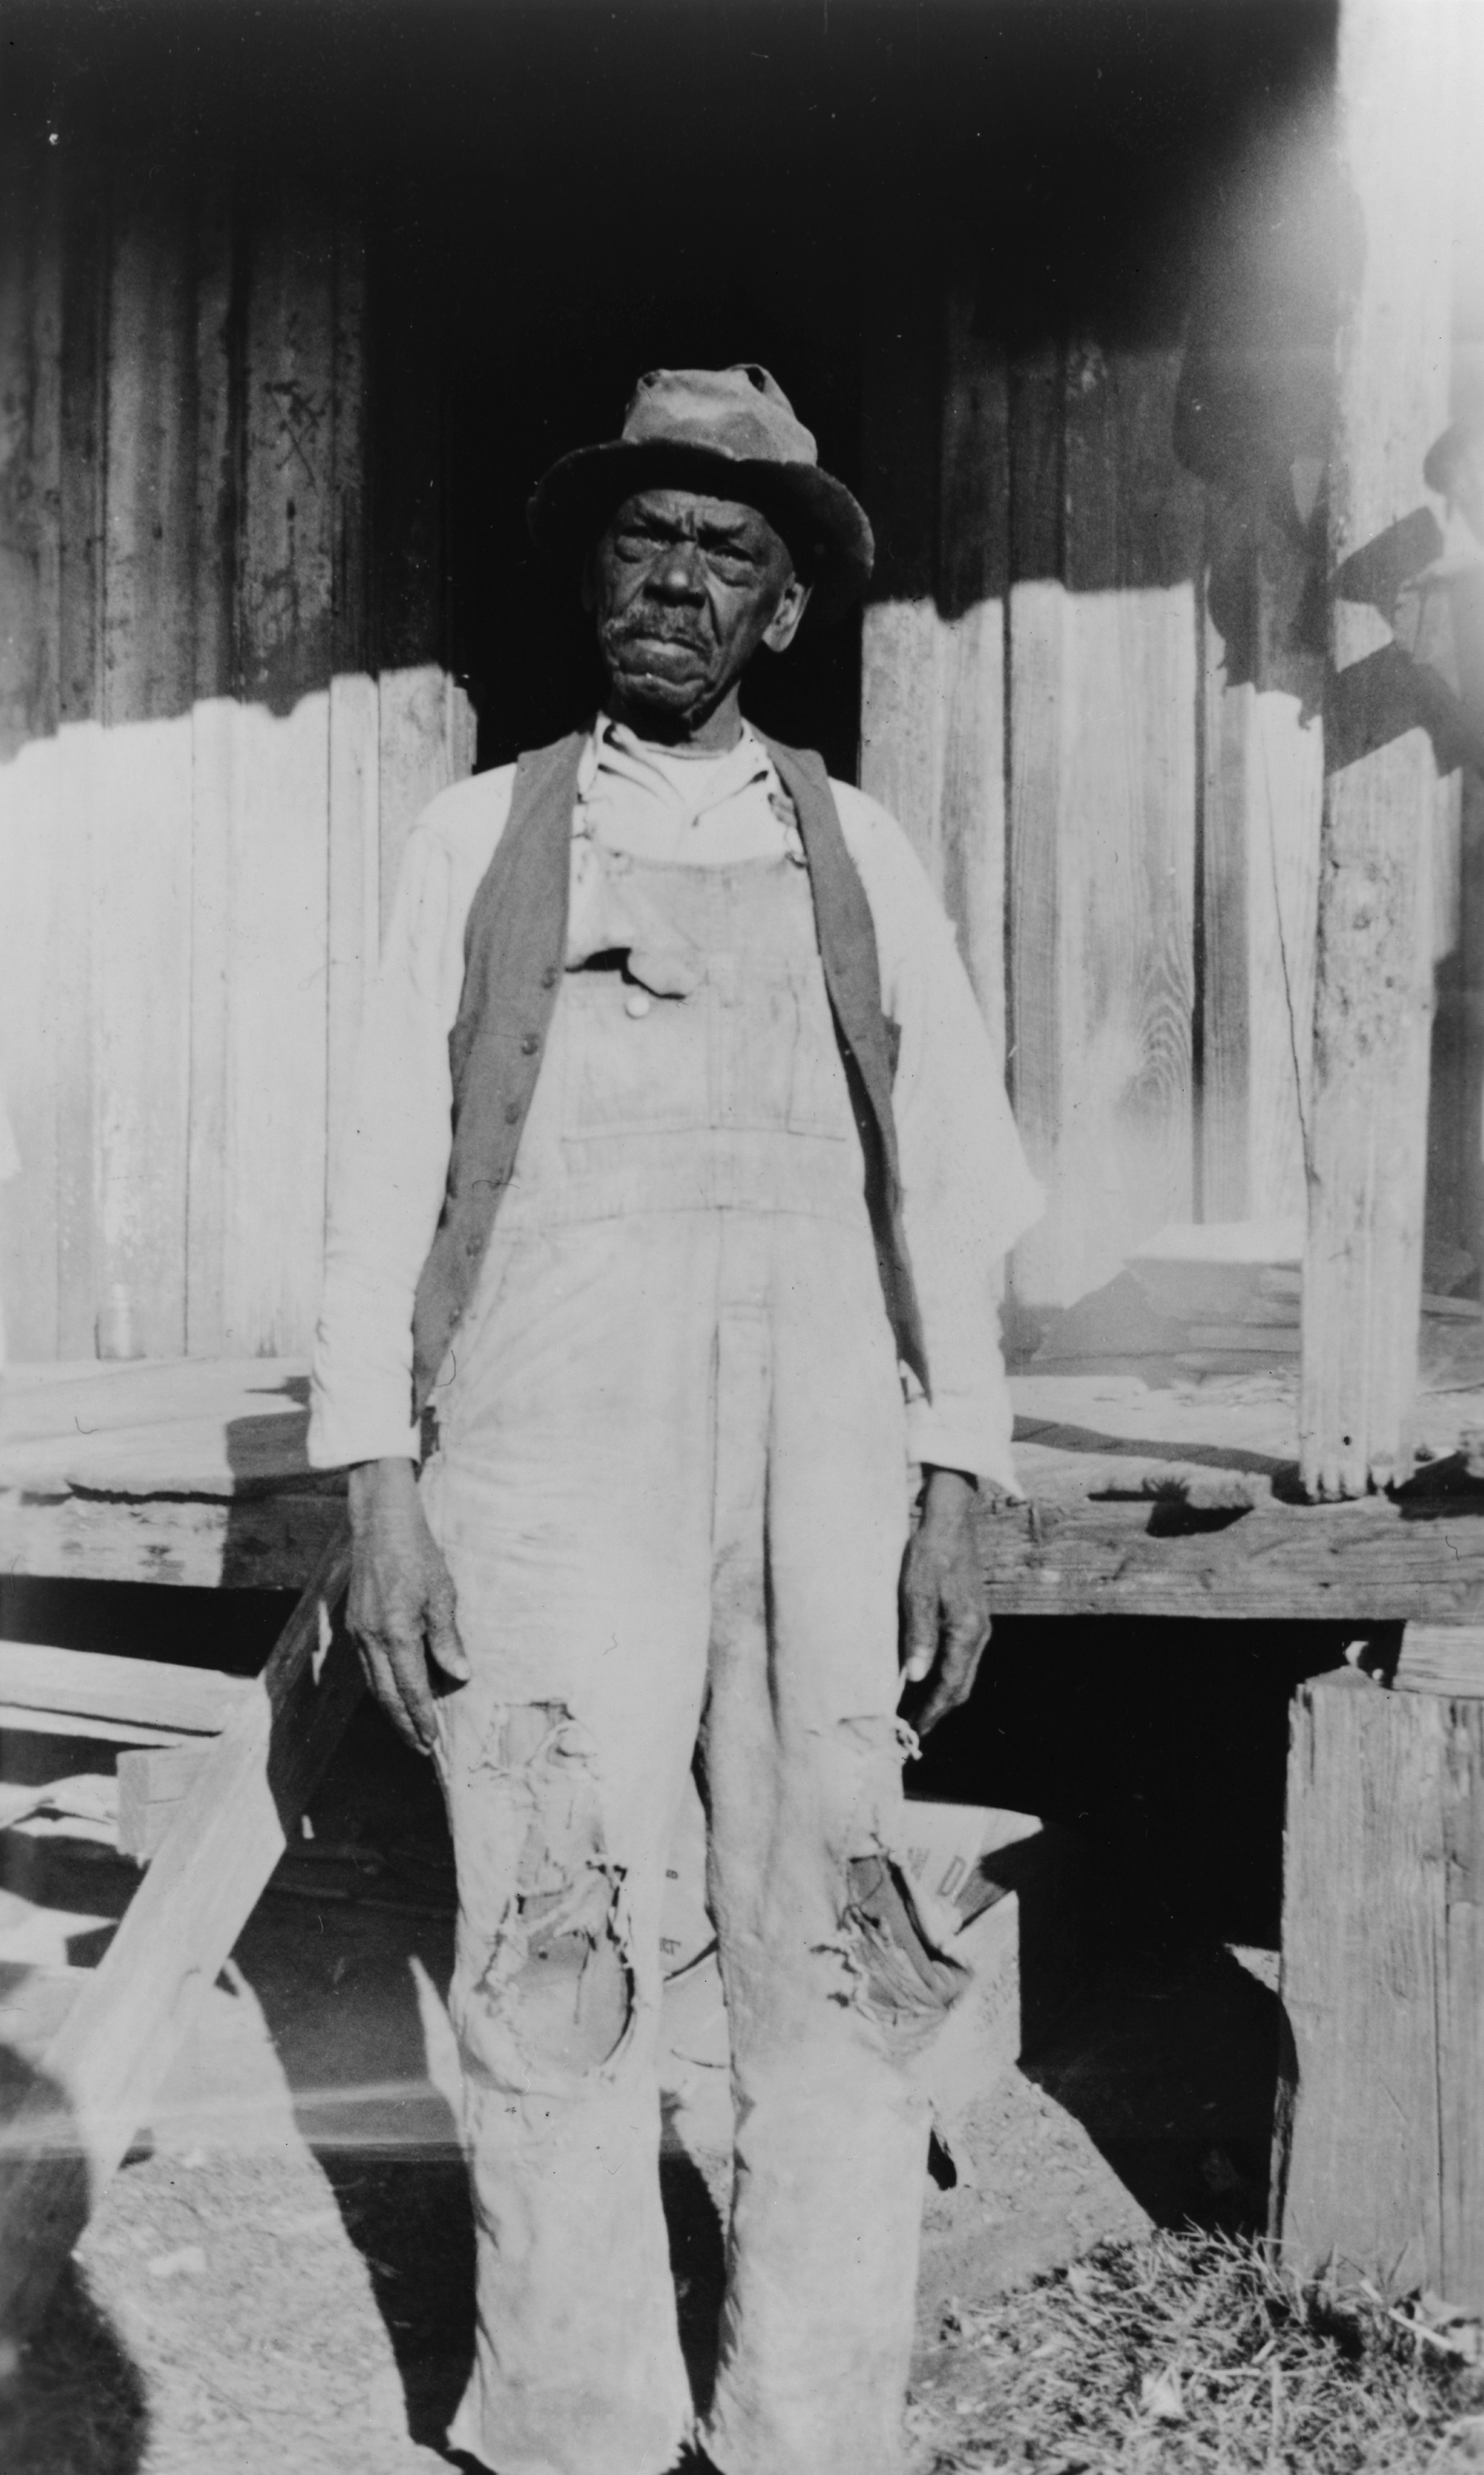
\includegraphics[width=90mm]{./imgs/solwaltson_recorte.jpg} \label{img3}
\caption{Sol Walton}
%\end{minipage}
\end{figure}

\subsection{Sol Walton, narrativas do Texas, Parte \versal{IV}, página 128}
\label{ref275}

``O primeiro trabalho que eu fiz na escravidão foi levar água e o almoço
para os peões, em baldes de cabaça. A gente não tinha balde de lata
naquela época. Os peões trabalhavam de sol a sol, e se o feitor visse
eles se afrouxando, ele praguejava e às vezes batia com um relho. Vi
eles levarem relhadas até a camisa ficar grudada nas costas. Vi minha
mãe ser chicoteada por gritar em um culto dos brancos. O velho senhor
tirou a roupa de cima dela e castigou com um relho. Vários e vários 
deles levaram relhadas só porque podiam levar chicotada. Alguns donos
não davam de comer para os peões e batiam em quem pedia comida''.

\subsection{Martha Allen, narrativas da Carolina do Norte, Parte~I,~página~14} \label{ref06}

``Minha mãe pertencia a Tom Edward Gaskin e não comia nem metade do que
devia. A cozinheira dava de mamar para os bebês enquanto cozinhava para
as mães poderem trabalhar no eito, e todas as mães tinham que meter os
bebês pela porta da cozinha no caminho. Ouvi mamãe dizer que elas iam
para o trabalho sem desjejum e que quando colocava o bebê na cozinha,
ela passava pelo balde dos restos e tomava os restos de uma cabaça com
cabo comprido.

O capataz não podia ser mais ruim, e os escravos levavam surras
horríveis''.

\paragraph{Comentário}\quad
{\small
Alguns senhores permitiam que os escravizados qualificados ``se
alugassem'', ou seja, cobrassem por serviços prestados a terceiros. Essa
prática era mais comum entre proprietários com residências urbanas, pois
escravos"-artesãos tinham mais facilidade para encontrar trabalho
remunerado na cidade. Nesse sistema, o cativo era obrigado a pagar ao
seu proprietário uma determinada soma toda semana, mas se ganhava mais
do que esse valor, ele podia ficar com o lucro. Além dessa possível
vantagem, os artesãos que se alugavam nas cidades muitas vezes tinham
mais liberdade pessoal.

Na agricultura, o sistema de trabalho mais comum era o trabalho em
turma, no qual um grupo de cativos trabalhava sob a supervisão de um
feitor ou capataz. Mas alguns proprietários, especialmente em áreas de
rizicultura, usavam um ``sistema de tarefas'', no qual uma determinada
quantidade de trabalho, chamada de ``tarefa'', era alocada a cada
indivíduo. Quando se completava a tarefa, o escravizado podia usar o
resto do seu tempo como bem entendesse. Para os trabalhadores mais
rápidos, esse sistema oferecia uma óbvia vantagem em potencial.
}

\subsection{George Lewis, narrativas da Geórgia, Parte \versal{III}, página 47}
\label{ref171}

{[}Viveu em situação de escravidão na Flórida.{]} ``Em termos de trabalho, todos os
membros do clã Lewis se saíram muito bem. O pai (\ldots{}) era um
construtor de navios experiente e tinha permissão para se alugar para
quem precisava dos seus serviços. Ele também tinha permissão para alugar
os seus filhos que tivessem idade o suficiente para trabalhar. Ele
precisava apenas pagar uma determinada porcentagem da sua renda ao seu
senhor e à senhora dos seus filhos''.

\begin{figure}[]
%\begin{minipage}{0,4\textwidth}
\centering
 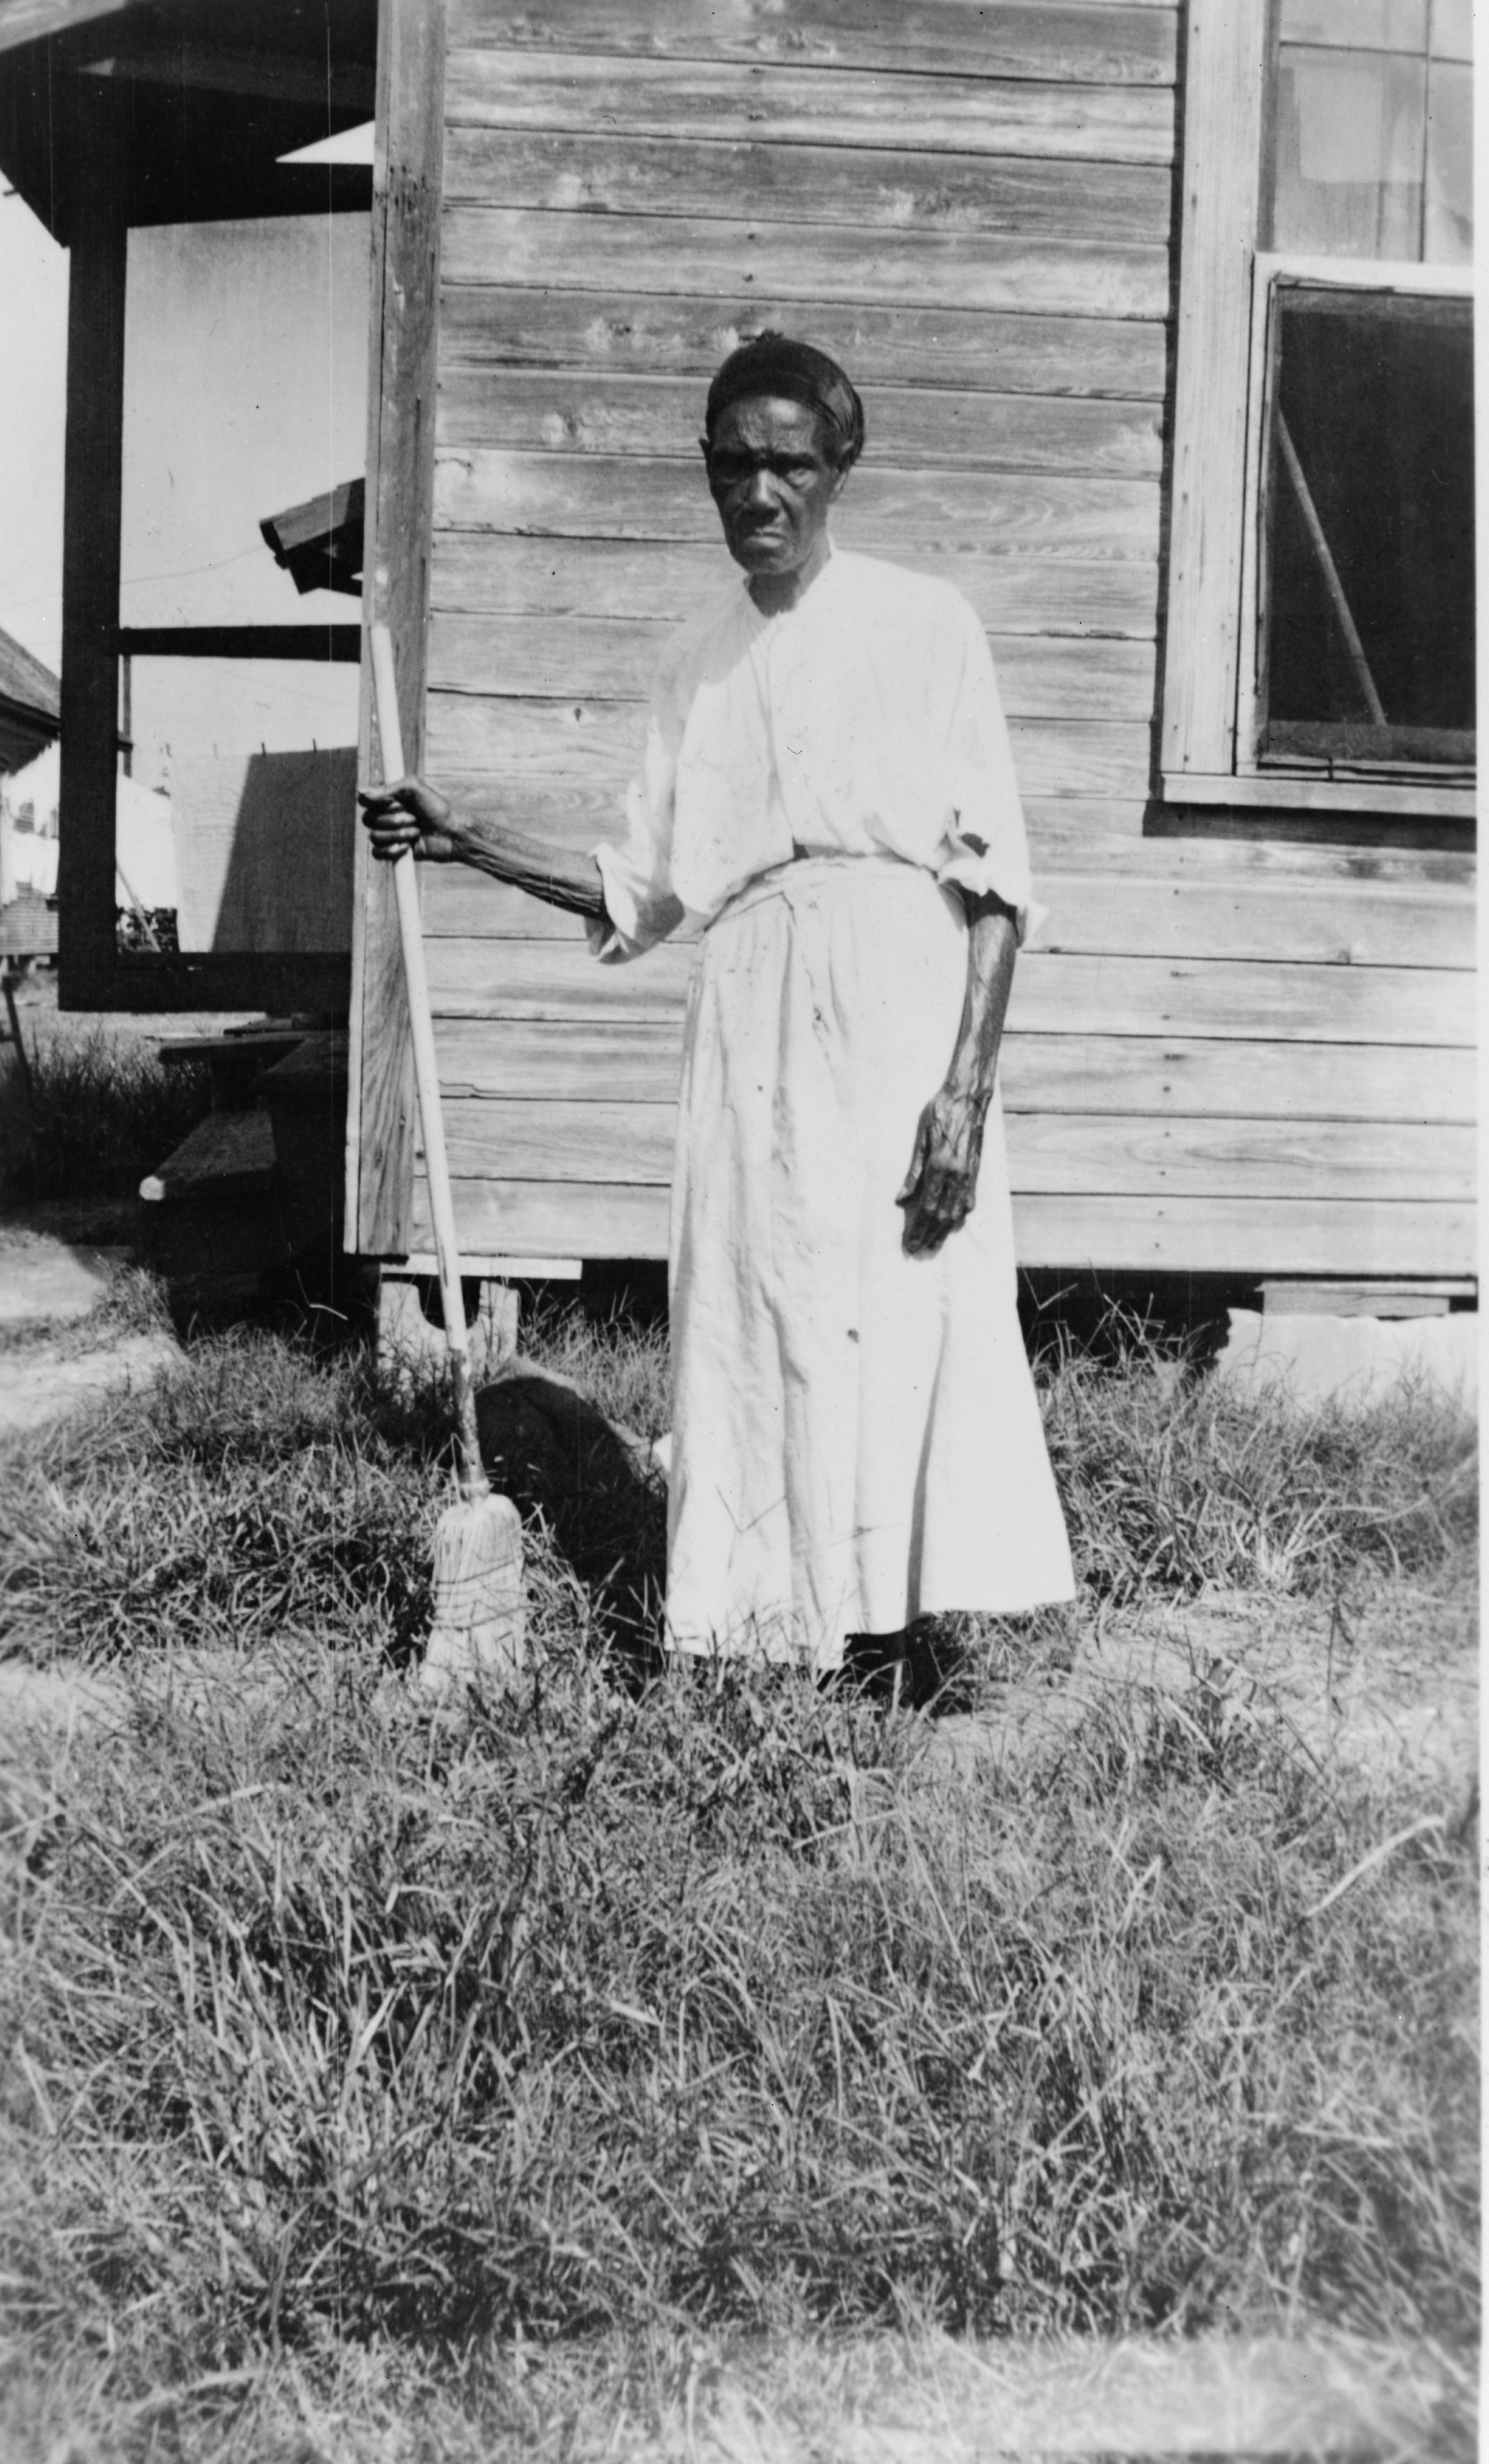
\includegraphics[width=90mm]{./imgs/clarabrim_recorte.jpg} \label{img4}
\caption{Clara Brim}
%\end{minipage}
\end{figure}

\subsection{Clara Brim, narrativas do Texas, Parte I, página 148} \label{ref33}

{[}Viveu em situação de escravidão na Luisiana e o seu senhor era um caso raro de usar o %Pensar em outra construção para a frase
sistema de tarefas no cultivo de algodão.{]} ``Quando os escravos iam
trabalhar, ele dava a tarefa. Tanto trabalho, tantas linhas de algodão
para cortar ou de milho para capinar. Quando terminavam, eles podiam
fazer o que quisessem. Ele dava as tarefas na segunda"-feira. Alguns
terminavam tudo na quinta de noite. Depois, eles podiam alugar seu tempo
e receber por isso''.

\subsection{Prince Smith, narrativas da Carolina do Sul, Parte~\versal{IV},~página~117}
\label{ref247}

``Tinha três tipos de dia de trabalho na fazenda: um é a tarefa inteira,
o que quer dizer um homem inteiro ou uma pessoa no auge. Ele recebia duas
tarefas pelo dia de trabalho. Uma tarefa ia de vinte e quatro a vinte e
cinco carreiras entre os algodoeiros, que tinham dez metros e meio de
comprimento e sete e meio de largura. Os homens três quartos recebiam
uma tarefa só, que consistia em doze linhas. Todas as crianças pequenas
estavam nesse grupo. Os homens de metade eram os escravos velhos que
faziam meia tarefa para os seus dias de trabalho. Quando chegava a hora
de apanhar algodão, os três quartos tinham que enfardar treze quilos e
meio por dia de trabalho e os homens de metade, nove quilos. Os que
cuidavam do descaroçador incluíam só os homens três quartos''.

\subsection{Tio Gabe Lance, narrativas da Carolina do Sul, Parte~\versal{III},~página~92}
\label{ref168}

``O senhor era bom. Dava bastante de comer. Tarefas razoáveis. A tarefa
era de mil a dois mil metros quadrados. Para abrir valas, dez medidas.
Tinha que limpar o lodo. Ir tirando água até enxergar as pegadas.

Aqueles arrozais todos eram um pântano só. A gente da escravidão abriu
canais e escavou valas e derrubou aquelas árvores\ldots{} e abriu vala
pela mata virgem. Foi tudo limpado para a gente da escravidão plantar
arroz''.

\subsection{Cato Carter, narrativas do Texas, Parte~I,~páginas~204~e~206} \label{ref51}

``Nossa fazenda tinha 600 hectares, tudo num bloco só, e além dos campos
de algodão e milho e arroz e cana que a gente plantava nas baixadas, a
gente tinha verdura, ovelha e boi. (\ldots{}) Nunca tive do que reclamar
de como era tratado, mas alguns negros odiavam a época de fazer melado,
porque tinham que trabalhar até a meia"-noite fazendo melado e acordar
igual às quatro da manhã. De sol a sol era para os negros do eito''.

\subsection{Ellen Betts, narrativas do Texas, Parte I, páginas 79, 76, 79} \label{ref25}

``Meu Deus, mas eu vi milhares e milhares de barris de açúcar e
caldeirões de melado quando era nova. Só Deus sabe quanta cana o velho
senhor tinha. Para quem corta a cana não parece muito, mas para quem
trabalha todas as horas nisso, aqueles canaviais bem que parecem que vão
de uma ponta à outra do mundo. O senhor mandava tonel atrás de tonel rio
abaixo. Eu via os barcos descendo o rio com cartazes enormes que diziam
`Vende"-se Melaço' nos lados. E ele plantava um mundo de arroz e batata e
milho e amendoim também. (\ldots{}) Quando as negras tinham que cortar
cana o dia inteiro até a meia"-noite e depois também, eu dava de mamar
para os bebês delas e cuidava das criancinhas brancas também. (\ldots{})
O senhor era muito bom para as moças e os negros que cortavam a cana.
Quando eles terminavam de fazer açúcar, ele distribuía uma bebida que se
chama `pêssego com mel' para a mulherada e uísque e conhaque para os
homens. E tinha dança e cabriolagem aos montes''.

\subsection{Maggie Black, narrativas da Carolina do Sul, Parte~I,~páginas~58--59} \label{ref26}

``Eles faziam todo o tecido que usavam lá mesmo na plantação. Se usava
algodão e lã o tempo inteiro naquela época. A Madame, claro, ela podia
comprar as sedas mais refinadas, porque quase tudo dela vinha do
exterior. Moça, ainda vejo minha velha mãe, trabalhando naquela roda de
fiar, vejo tão bem como se aquele dia fosse o dia de hoje. Ela sentava
com aquela roda velha, pegava uma lançadeira e atirava para lá e para
cá, puxando aquele negócio para ficar mais e mais apertado. Era vapt,
vupt, e tinha que trabalhar com os pés também. Era assim que faziam
tecido naqueles tempos.

Querida, as pessoas tinham que trabalhar duro por tudo que tinham
naqueles tempos. Eles plantavam o próprio arroz lá mesmo na plantação.
Tinha que plantar nas partes do terreno que eram mais úmidas que o resto
das terras. Tinha que deixar o arroz ficar bem maduro e depois cortavam
ele, então vinha um daqueles dias de bater bem o arroz. Montes de
pessoas vinham das fazendas ajudar a bater o arroz. Eles só pegavam o
arroz e batiam em algum cavalete que tinham montado em algum lugar da
fazenda. Querida, era um cavalete igual a esses que se vê os
carpinteiros usando por aqui hoje em dia. Eles tinham centenas de
alqueires daquele arroz. Quando terminava, eles faziam um jantarzão para
todo mundo que tinha batido o arroz. Davam todo o arroz e os barris de
bebida que se podia querer. Ah, a música era das boas. Todo mundo
chacoalhava os ossos e batia palmas com aquela melodia.

Depois pilavam o arroz lá mesmo na fazenda, arrumando ele bem bonito.
Então tinham que levar para o moinho. Pois eles tinham um bloco lá no
pátio, com um furo enorme no meio, onde despejavam o arroz. Depois
pegavam essas coisas chamadas de pilão e batiam nele para tirar os
talos. Não se tinha esse arroz bonitinho como se vê hoje, porque não era
branco que nem o arroz que se tem hoje, mas era um arroz bem doce,
querida, um arroz bem doce''.


\paragraph{Comentário}\quad
{\small
Os entrevistados lembram"-se de algumas épocas mais felizes, quando o
trabalho na fazenda diminuía ou as pessoas podiam celebrar a colheita. A
tarefa de separar o milho da palha muitas vezes era uma atividade
coletiva e um momento para se divertir. Eles também evocam com
carinho dos poucos dias de descanso que recebiam no Natal.
}

\subsection{Jenny Proctor, narrativas do Texas, Parte~\versal{III},~páginas~209,~214,~210}
\label{ref216}

``Eu ouço falar dos bons tempos da escravidão, mas nunca vi bons tempos
naquela época. O nome da minha mãe era Lisa e quando eu era bem
criancinha, eu escutava o feitor indo de cabana em cabana, começando às
três da madrugada, e quando chegava na nossa cabana ele dizia `Lisa,
Lisa, sai daí e faz o desjejum'. Minha mãe, ela era cozinheira, do meu
pai não lembro nada. (\ldots{}) Eu cuidava das crianças quando era
menininha e tentava limpar a casa igual a velha senhora mandava. Logo
que fiz dez anos, o velho senhor disse\ldots{} `Leva essa crioula para o
algodoal'. (\ldots{})

Todo Natal que a gente tinha é que o velho senhor matava um porco e 
nos dava um pouco da carne. A gente achava isso bom, e o Natal durava de
acordo com a tora de árvore"-do"-âmbar que cortavam e usavam de lenha no fundo
da lareira. Quando ela acabava de queimar, o Natal terminava. Então pode
saber que a gente passava o ano inteiro procurando a maior
árvore"-do"-âmbar que desse. Quando não achava, a gente pegava um
carvalho, mas esse não durava o suficiente, só uns três dias em média,
quando não era preciso trabalhar. O velho senhor gostava de atirar nó de
pinho na lareira para acabar com o Natal de uma vez e nos mandar de
volta para o trabalho.

A gente debulhava milho às vezes, mas os brancos se divertem e os negros
é que trabalham. Não tínhamos que apanhar algodão, só apanhar o nosso
próprio. (\ldots{})

{[}Uma vez, ela foi açoitada por roubar e comer um biscoito e o senhor
ficou furioso com o feitor.{]} `Ela não vai ter como trabalhar por uma
semana, teria pago por vários biscoitos nesse tempo'. (\ldots{})
Tínhamos uma flanela vermelha para o inverno sob as roupas. A velha
senhora dizia que um negro doente custava mais do que a flanela''.

\subsection{Ed McCree, narrativas da Geórgia, Parte~\versal{III},~página~63,~60--61}
\label{ref186}

``Quando chegava o inverno, os homens tinham bastante milho para
debulhar e as mulheres tinham acolchoados para fazer. Tinha uma linha de
milho para debulhar comprida como se fosse daqui até a Avenida Milledge.
O velho senhor colocava uma turma de negros em cada ponta da linha e
tinha uma corrida acirrada entre as duas turmas para ver quem chegava no
meio primeiro. Sempre tinha um banquete esperando por eles quando a
última espiga fosse debulhada. E os acolchoados! Olha, senhora, o que é
que um negro velho vai saber de uma coisa que era só das mulheres?

A época de apanhar o algodão era uma beleza. Eles apanhavam algodão no
luar e então faziam um banquete de churrasco de gado, ovelha e porco,
tudo regado a uísque do bom. Quando a comida acabava, alguns dos negros
tocavam rabeca e banjo para os outros dançarem até se acabarem.

O velho senhor John McCree era um branco bom, estou contando
a verdade, porque não sou de contar a outra coisa. (\ldots{})

Tinha mais de 400 hectares aquele fazendão. Era uma terra das grandes, e
recheada de negros. Não sei dizer quantos, já esqueci. Dava para escutar
a corneta do feitor que tocava para acordar os escravos a quilômetros de
distância. Ele os acordava bem antes do sol nascer e colocava eles para
trabalhar no eito assim que conseguissem enxergar o trabalho que tinha
para fazer. Nem me fale daquele feitor surrando os negros. Ele batia por
quase qualquer coisa. Para que iam precisar de cadeia se tinha aquele
feitor para descer aquele relho de couro cru?''.

\subsection{George Strickland, narrativas do Alabama, página 361}
\label{ref256} 

``Debulhar milho era o melhor de tudo. O velho senhor levava um garrafão
e deixava eles bem bêbados, e quando ficavam cheios eles atiravam ele
para cima e para baixo, carregavam ele para tudo quanto é lado e davam
gritos. Depois começava a diversão, eles tocavam uma cabaça velha com
crina de cavalo, serrote e faca de mato. Eles corriam a mão para cima e
para baixo no serrote para mudar a música, e o líder ficava em cima da
pilha de milho, cantando enquanto todos os outros imitavam''.

\pagebreak
\thispagestyle{empty}

\movetoevenpage
\thispagestyle{empty}
\begin{absolutelynopagebreak}
\begin{vplace}
\begin{figure}[H]
\begin{adjustwidth}{-1.8cm}{}
  %\centering
  \vspace*{-2cm}
  %\hspace{-0.5cm}
  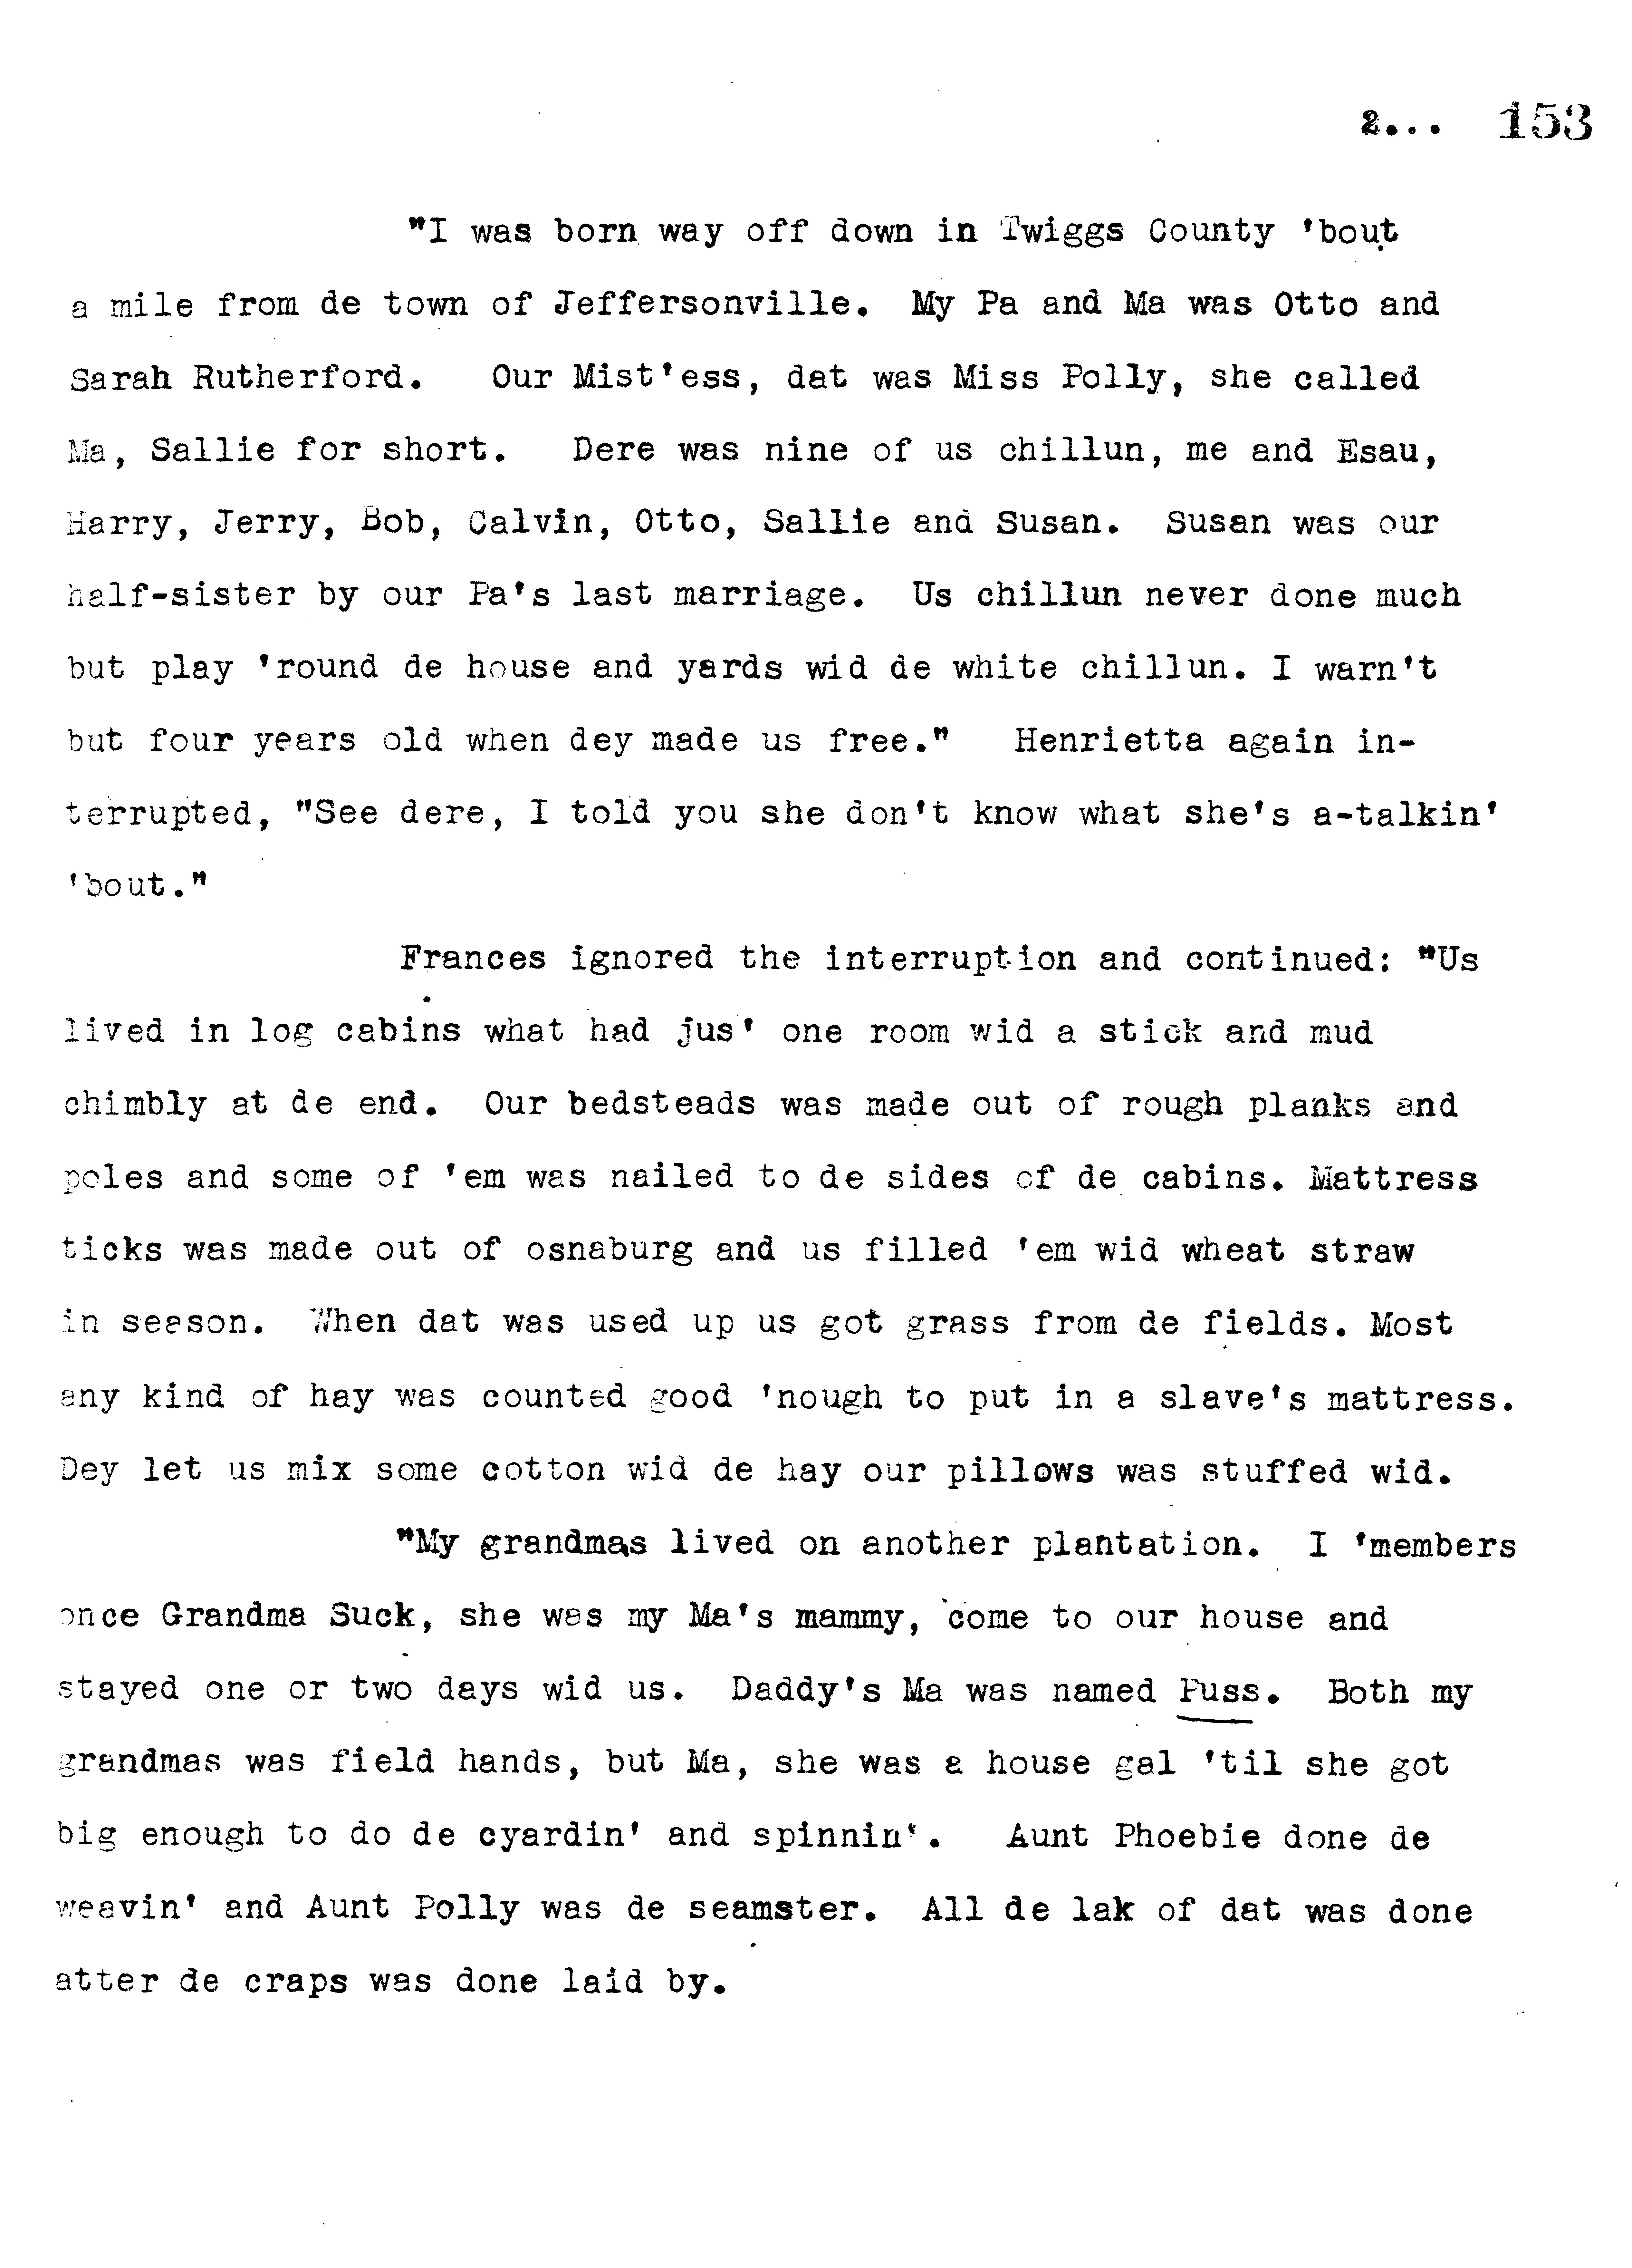
\includegraphics[width=130mm]{./imgs/Cap2.jpg}  
  %\hfill
\end{adjustwidth}
  \caption{Frances Willingham, narrativas da Geórgia, Parte \versal{IV}, página 153}
\end{figure}
\end{vplace}

\end{absolutelynopagebreak}

\chapter{Condições de vida}
%\addcontentsline{toc}{chapter}{{\large\versal{II.}} Condições de vida}
%\hedramarkboth{Condições de vida}{}

\subsection{Frances Willingham, narrativas da Geórgia, Parte~\versal{IV},~página~153--54,~156,~158}
\label{ref296}

``A gente morava em choupanas de um quarto só, com uma chaminé de galhos
e barro na ponta. Os estrados das nossas camas eram feitos de tábuas
grosseiras e varas, e algumas eram pregadas nas paredes da choupana. A
capa dos colchões era feita de osnaburgo e a gente enchia elas de palha
de trigo quando estava na estação. Quando a palha acabava, a gente
trazia grama do eito. Praticamente qualquer forragem era boa o
suficiente para se enfiar no colchão de um escravo. Eles nos deixavam
misturar um pouco de algodão com a palha usada para estufar os nossos
travesseiros.

Não, senhora, ninguém nunca deu dinheiro para criança escrava
nenhuma naquela época. Eu nunca tive até depois de a gente ganhar a
nossa liberdade. Eu costumava ver o velho senhor contando dinheiro, mas
os escravos nunca receberam nada daquilo.

Nosso velho senhor era um homem rico e poderoso e acreditava em nos dar
bastante de comer. Não era nada de fino, mas era comida boa e simples,
que enchia a barriga e nos mantinha bem. Tinha pão de milho e carne,
tudo quanto é tipo de verdura, milho assado e tantos tipos de legume que
dava para passar o dia todo contando. O senhor tinha uma horta das
grandes onde ele plantava de tudo, exceto repolho e tomate. Ele dizia
que essas coisas não prestavam para ninguém. O senhor deixava papai
caçar o suficiente para trazer vários gambás, guaxinins, coelhos e
esquilos. A gente cozinhava eles como se cozinha hoje, mas ninguém tinha
fogão naquela época, então era tudo cozinhado em lareiras abertas, com
uns panelões e frigideiras de cabo comprido que tinham umas tampas bem
pesadas. Eu vi mamãe limpar muitos e muitos gambás nas brasas. Depois
ela escaldava eles e tirava as entranhas. Ela aferventava e depois
assava eles e quando levava para a mesa cercado de batata"-doce no prato,
que coisa boa de comer era aquilo. Papai pescava no riachinho, porque os
escravos não tinham permissão para sair da fazenda para essas coisas.

Eu nunca tive um dia de escola na minha vida, porque quando era
pequena os negros não podiam aprender a ler e escrever. Ouvi minha mãe
dizer que o pastor negro lia a Bíblia, mas nunca vi ele fazendo isso,
porque nunca fui à igreja quando era pequena.

De noite, quando os escravos chegavam do eito, as mulheres
limpavam a casa depois de comer, então lavavam a roupa e penduravam elas
para secar de manhãzinha. Os homens comiam, sentavam para conversar uns
com os outros e depois iam para a cama. Na nossa fazenda, todo mundo
trabalhava no domingo até as três ou quatro da tarde, e se o trabalho
era muito eles trabalhavam até a noite cair, como se fosse um dia
qualquer. Domingo de noite, os mais novos se juntavam para fazer festa.
Eles dançavam, brincavam, bebiam, essas coisas. O velho senhor não era
duro com eles, mas só dava aquela uma noite para eles brincarem. No
domingo, ele dava passes para quem queria ir à igreja ou fazer
visitas.

É claro que o senhor botava os escravos para debulhar milho,
descascar milho, apanhar algodão e costurar acolchoados. Ele tinha
vários e vários pomares de nogueira"-pecã, castanheira, nogueira"-comum,
nogueira"-amarga, eucalipto e castanheiro"-da"-Califórnia. Depois que as
nozes eram juntadas, o velho senhor vendia ela para os grandões na
cidade. É por isso que ele era tão rico. Depois que tudo isso era
juntado e cuidado, ele fazia um festão para os escravos, com bastante
para beber, então deixava eles descansarem alguns dias antes do trabalho
começar de novo''.

\paragraph{Comentário}\quad
{\small
As condições da vida escrava no sul dos Estados Unidos
dependiam das atitudes dos senhores, mas nenhum escravizado vivia em nada
que se poderia chamar de luxo. Para a maioria, suas cabanas
eram pequenas, de madeira grosseira, com as frestas entre as toras
tapadas com barro. Alguns tinham que dividir a cabana com outra
família. Na maioria delas, o chão era de terra, e quando havia uma
lareira, a chaminé era feita de ramos e lama seca. As camas eram
rudimentares e os colchões eram forrados de palha ou barba"-de"-velho.

A maioria dos entrevistados nas narrativas do \versal{FWP} parecem lembrar que a
quantidade de comida recebida era adequada, mas que suas dietas eram
quase sempre monótonas e nem sempre continham as quantidades necessárias
de vitaminas e nutrientes. A base da dieta escrava era
banha de porco, farinha de milho, verduras e alguns legumes. Alguns
escravistas, mas nem todos, criavam bois e forneciam carne de gado ou de
outros animais. Em algumas fazendas, a escravaria passava fome. Aqueles
que tinham permissão para cultivar uma roça podiam complementar a sua
dieta, e caçar e pescar também ajudava a melhorar a situação.

As roupas eram simples e grosseiras e nem sempre adequadas para
climas mais frios. Quando os escravizados tinham sapatos, estes normalmente
eram feitos de couro duro e pouco confortáveis. Para melhorar as suas
vestimentas, muitas cativas recorriam à sua herança cultural africana e
cobriam suas cabeças com lenços coloridos. Mas quase tudo nas roupas,
assim como acontecia com a alimentação e a moradia, dependia do
proprietário, e alguns escravizados sofriam por causa de senhores hostis ou
mesquinhos.

O aspecto das condições de vida que mais chama a atenção é a
tendência dos escravistas de castigar seus trabalhadores com surras e
chibatadas, ou de não fazê"-lo, e outro capítulo se concentrará mais
nesse assunto. Contudo, os entrevistados também se lembram de diversas outras
formas de maus"-tratos e privações que eram parte da vida em cativeiro.
}

\subsection{Sallie Carder, narrativas do Oklahoma, páginas 27--28} \label{ref48}

``Não, senhor, nós nunca tivemos dinheiro quando eu era escrava. A gente
não tinha nada de nada. O que se comia era verdura, pão de milho e
fogaça. As únicas vezes em que ganhava um biscoito era quando alguém
fazia uma coisa de errado e a minha senhora dava um biscoito amanteigado
para quem contasse quem era o culpado. (\ldots{})''

\subsection{Eli Coleman, narrativas do Texas, páginas 236--37}

{[}Viveu em situação de escravidão no Kentucky.{]} ``A gente fazia tudo quanto é tipo de trabalho, cortando algodão e
rachando tora, cortando pedra e trabalhando na plantação de tabaco. A
gente cortava o tabaco e pendurava no barraco para secar. Era preciso
pendurar pelo restolho.

Tínhamos bastante de comer, como pão de milho. O milho era ralado à mão
e cozinhado nas cinzas, sem sal nem bicarbonato nem essas coisas finas
que se bota no pão hoje em dia.

Tinha gambá e coelho e a gente cozinhava diferente do que se faz hoje.
Um caldeirão enorme ficava pendurado sobre a lareira de pedra. A comida
que se cozinha assim ainda é boa. O senhor Brady sempre nos dava
bastante da horta. Ele sempre nos dava comida forte e reforçada, que nem
se cuida de um cavalo, se ele é bem bom''.

\subsection{Josephine Bristow, narrativas da Carolina do Sul, Parte~I,~páginas~98--100} \label{ref34}

``Eu era bem pequena naqueles tempos e até onde lembro, a gente morava
na senzala da fazenda do velho senhor lá no interior. Toda manhã, nós
pequeninos íamos para um lugar no alto do morro, a leiteria, e
ganhávamos o nosso leite entre as refeições enquanto os mais velhos
estavam trabalhando. Ah, eles tinham uma velha que cuidava de nós
durante o dia. A velha que nos cuidava, o nome dela era Mary Novlin. Meu
Deus, o Sr. Gibson, ele tinha uns fazendões, e minha mãe e meu pai
trabalhavam nas fazendas. Sim, senhora, minha mãe e meu pai, eu nunca
sabia quando eles iam chegar em casa de noite, de tão tarde que era. A
velha cuidava de tudo para nós o dia inteiro, e ainda cozinhava para nós
ao mesmo tempo que nos cuidava. Ora, ela fervia para gente canjica de
farinha de milho e quase sempre nos dava com leite no desjejum. Depois,
eles tinham uma horta bem grande, então ela cozinhava ervilha para nos
dar bastante sopa com um pão de forno que nem este. Ah, mas quem
trabalhava no eito, esses comiam as refeições quando podiam. Tinha que
cozinhar no meio da noite, às vezes antes do dia nascer, porque eles
levavam as rações de almoço com eles para o campo. Mais ou menos
cozinhavam no eito. Sim, senhor, eles levavam as panelas consigo e
cozinhavam lá mesmo no eito enquanto estavam trabalhando. Ferviam água e
assavam pão também. Não sei quanto tempo eles tinham que trabalhar,
senhora, mas eu ouvia eles dizerem que trabalhavam muito, fosse frio ou
quente, fizesse sol ou chuva. Tinham que capinar os algodoeiros e
apanhar algodão e tudo mais. Não sei bem, minha senhora, mas os brancos,
eles achavam que não faltava bastante gente negra e Deus não criou eles
para trabalharem. Os brancos daquele tempo, sabe, eles faziam a gente
negra trabalhar.

O povo costumava fiar e tecer, meu Deus! Igual a hoje, quando estava
nublado e chovendo, eles não podiam trabalhar no eito, então era dia de
fiar. Ai, você ouvia aquela coisa rodando e eu ainda lembro de ficar ali
parada, querendo fiar feito louca, eu nunca sabia o que fazer. Não
demorou para eu saber usar a lançadeira e tecer também. Eu tinha uma avó
que quando pegava naquela roda, ah, ela sabia muito bem o que fazer. Os
brancos costumavam dar aos negros uma tarefa de fiar e ela sabia fiar
como ninguém. Sim, senhora, vou lhe contar, se fazia o tecido mais lindo
do mundo naqueles tempos. O povo de antigamente tinha um tipo de corante
chamado índigo e eles tingiam o tecido, nunca se viu coisa mais bonita.

Depois eu lembro que precisavam debulhar milho alguns dos dias e ninguém
trabalhava no eito nesses dias. Meu Deus, eram uns dias de comilança,
esses. Levavam uma panelona lá para dentro do celeiro, onde estavam
debulhando o milho, e ferviam ela cheinha até a borda, com ervilha e
arroz e couve. Assavam um pão bem grande também, e muitas vezes se
guardava uma meia pipa para esses dias''.

\subsection{Tom Holland, narrativas do Texas, Parte~\versal{II},~páginas~144,~145}
\label{ref147}

``Eu cortava algodoeiros, arava e rachava toras, depois passei a
cavalgar. Naquele tempo, eu era capaz de domar o cavalo mais xucro que
já levantou poeira no Texas, mas nunca fui muito valioso por causa do
meu olho de vidro. Não lembro de como fui acabar com ele, mas aqui
estou. Eu ganhava um dólar ou cinquenta centavos para montar um cavalo
selvagem nos tempos da escravidão, e o senhor me deixava ficar com o
dinheiro. Eu comprava tabaco e doces, e se o senhor me pegava com tabaco
eu era açoitado, mas sempre escapulia e comprava fumo de mascar.

A gente sempre tinha bastante de comer, do que tinha de comer naquele
tempo, e era bom, bastante carne de caça e pão de milho assado nas
cinzas. A carne se assava na fogueira, e tinha bastante gambá, coelho e
peixe. A roupa era um camisão aberto até embaixo na frente, mas nunca vi
sapato até bem depois da liberdade. Em tempo frio, o senhor curtia
bastante couro e a gente fazia roupas quentes. Minha roupa de casamento
foi um camisão branco. Nunca tive sapatos, casei descalço.

(\ldots{}) Eu vi escravos sendo vendidos e leiloados, porque eu mesmo
fui vendido para o lance mais alto. O senhor me vendeu para William
Green logo antes da guerra por cem acres de terra a um dólar por acre.
Ele achava que eu nunca serviria para nada, porque tinha esse olho de
vidro, mas ainda estou vivo e sou um negro muito bom para a minha
idade''.

\subsection{Louise Everett, narrativas da Flórida, páginas 128--29}

``A vida na fazenda dos McClain era uma rotina monótona de trabalho
constante que ia da manhã à noite. Os escravos precisavam acordar ainda
de madrugada, quando repicava o sino da casa grande. Após um desjejum
apressado de carne de porco fritada na banha e pão de milho, eles
trabalhavam no eito até o sino tocar novamente ao meio"-dia, quando
comiam legumes cozidos, batata"-doce assada e melaço. Essa comida era
preparada em panelas de ferro com pernas embaixo, o que permitia que
fossem colocadas diretamente acima do fogo. Esses utensílios eram
pendurados sobre uma fogueira ou posicionados sobre um monte de brasas
quentes. Biscoitos eram um luxo, mas sempre que tinham pão branco, este
era cozinhado em outra caçarola mais espessa. Essa caçarola tinha uma
tampa coberta com brasas quentes para garantir que a parte de cima do
pão ficaria dourada.

As escravas não tinham tempo para os filhos. Quem cuidava deles era uma
velha senhora que os chamava duas vezes ao dia para dar ``licor de
panela'' (caldo de vegetais) e leite desnatado. Cada criança recebia uma
concha de madeira, que mergulhavam no cocho de madeira para se
alimentarem sozinhas. As crianças mais velhas alimentavam as mais novas,
jovens demais para segurar a concha.

`Big Jim' era tão rigoroso que os escravos eram forçados a trabalhar até
quando estavam doentes. Mães grávidas labutavam no campo até sentirem as
dores do parto. Não raro, os bebês nasciam na própria lavoura.

Não havia muito tempo para diversão na sua fazenda. Até crianças muito
pequenas recebiam tarefas. Elas procuravam ovos de galinha, recolhiam
erva"-dos"-cancros para fazerem corante, descascavam milho e levavam as
vacas para casa ao anoitecer. As menininhas tricotavam meias.

Não havia igreja nessa fazenda, e os pastores itinerantes a evitavam
devido à crueldade do proprietário. Os escravos raramente tinham
permissão de ir às igrejas vizinhas, e menos oportunidades ainda de
realizar seus próprios cultos''.

\subsection{George Womble, narrativas da Geórgia, páginas 185--87}
\label{ref307}

``No final da semana, todos os peões se reuniam no quintal do senhor,
onde recebiam uma determinada quantidade de comida, que supostamente
duraria até o final da semana. Essa ração era composta de 1,3 quilos de
carne gorda, um celamim de farinha e um litro de melaço. (\ldots{})
{[}Mas não era o suficiente, então os escravizados roubavam. Ver capítulo ``Resistência''.{]}

As crianças mais jovens eram alimentadas de um cocho de seis metros de
comprimento. Sempre na hora das refeições, o senhor vinha supervisionar
a cozinheira cujo dever era encher o cocho de comida. No desjejum, o
leite e o pão eram misturados no cocho pelo senhor, que usava sua
própria bengala. No almoço e no jantar, as crianças recebiam caldo de
vegetais e pão, e às vezes leite misturado da mesma maneira. Todos se
mantinham afastados até o senhor terminar de misturar a comida e, dado o
sinal, corriam para o cocho, onde começavam a comer com as mãos. Alguns
até mergulhavam suas bocas no cocho para comer. Algumas vezes, os cães e
alguns dos porcos do senhor que corriam soltos no pátio se dirigiam ao
cocho para participar da refeição. O Sr. Womble afirma que eles não
tinham permissão para bater em nenhum desses animais de modo a
afastá"-los, então eles colocavam as mãos nos lados do rosto enquanto
comiam para protegê"-los das línguas dos intrusos. Durante a refeição, o
senhor caminhava de uma ponta à outra do cocho para garantir que a
situação estava como deveria''.

\subsection{Alice Baugh, narrativas da Carolina do Norte, Parte~\versal{II},~página~83}

{[}Relatando o que a mãe lhe contou.{]} ``O senhor Charlie e a senhora Mary eram bons para os cem escravos que pertenciam a eles. Davam casas boas, comida boa, roupas boas e muita
diversão. Eles debulhavam milho, faziam danças no salão e tinha cultos e
coisas assim o ano inteiro, e do Natal até o segundo dia de janeiro
tinham um feriado, com boi, porco e peru assado e todas as guarnições.
De sábado à manhã de segunda, os escravos ficavam de folga e tinham suas
roupas de domingo, o que era muito bom. O senhor sempre dava um papel\footnote{Permissão para sair
da fazenda depois do toque de recolher. Sem ela, o escravizado podia ser
pego e torturado por patrulheiros noturnos que faziam vigília a
cavalo.} para os patrulheiros não pegarem ninguém.

Eles subiam o rio para ir nas danças e coisas assim das outras fazendas
e adoravam cantar. Era isso que faziam quando voltavam para as cabanas
no final do dia. Os mais velhos cantavam e alguém tocava o banjo''.

\subsection{Henry Lewis, narrativas do Texas, Parte \versal{III}, página 10}
\label{ref176}

``O velho senhor tinha um campo bem grande dividido no traçado, e cada
escravo tinha uma parte para plantar o que quisesse, e o velho senhor
comprava a safra do escravo. Ele era bem bom para os escravos, e nos
dava roupas boas também, lã para o inverno e algodão para o verão. A
gente tinha seis mudas por ano, com roupa de baixo e tudo mais. Na
cabana ficava um baú para as roupas de domingo, com o resto pendurado em
um cabide.

A gente tinha bastante comida boa para comer, também. Carne de gado,
porco, toicinho, melado, açúcar e farinha não faltavam. Todos os gambás,
coelhos, peixes e outros bichos eram só para completar. Ele também nos
dava um barril de uísque todos os anos''.

\subsection{Henry Wright, narrativas da Geórgia, Parte~\versal{IV},~páginas~197--99}
\label{ref317}

``As roupas eram distribuídas uma vez por ano, geralmente em torno de
setembro. As roupas do ano geralmente eram compostas da seguinte forma:
um par de sapatos pesados, chamados de `chanca de negro'. Várias camisas
de tecido de fio cru, meias de lã e dois ou três pares de calças jeans.
As mulheres recebiam vestidos e saias de baixo prontas ou então tecido
simples para fazer essas vestimentas. Algumas das roupas eram compradas,
outras eram feitas na própria fazenda. As meias de lã eram tricotadas na
fazenda, assim como o tecido de fio cru era fabricado nela. Esse tecido
era tingido em uma mistura fervente de folhas verdes de nogueira ou
cascas de noz. Quando se desejava produzir tecido axadrezado, os fios
eram tingidos da cor desejada antes de serem tecidos. (\ldots{})

Essas roupas muitas vezes eram insuficientes para atender as
necessidades individuais. Com um sorriso amplo e uma sacudida quase
imperceptível da cabeça grisalha, o Sr. Wright contou que trabalhara
descalço na lavoura em tempo frio até sua pele rachar e as feridas
começarem a sangrar. Ele também contou como, para economizar seus
calçados, ele costumava caminhar distâncias mais longas descalço, com os
sapatos embaixo do braço. Os calçados eram polidos com uma mistura de
fuligem e melado. As crianças escravas mais jovens usavam uma única peça
de roupa, com buracos para braços e cabeça. A peça se assemelhava a um
camisolão. (\ldots{})

A comida dos escravos era toda cultivada na fazenda. No final da semana,
cada escravo recebia 1,3 quilos de carne (quase sempre de porco), um celamim
de farinha e um pouco de melado. O desjejum e o almoço normalmente
consistiam em carne frita, pão de milho e melado. As verduras costumavam
ser servidas no almoço. Às vezes, dava"-se leite com o jantar. Era
necessário mandar as refeições para os escravos na lavoura, que em geral
estavam longe demais da casa para poderem se deslocar até lá. Para
tanto, havia uma mulher que cozinhava para todos os escravos da lavoura
em uma cozinha localizada entre as cabanas dos escravos. O Sr. House
permitia que seus escravos cultivassem uma roça e criassem galinhas. Na
verdade, ele designava um pequeno terreno para cada um deles para esse
fim. Para o escravo, essa prática tinha dois benefícios. Em primeiro
lugar, ele podia variar sua dieta. Segundo, ele podia ganhar algum
dinheiro vendendo os produtos desse terreno na cidade ou para o `velho
senhor'. (\ldots{})

O café era feito tostando farinha e então colocando"-a em água fervente.
Para adoçar esse café, usava"-se melado. Uma iguaria que ele e os outros
escravos costumavam receber aos domingos era bolacha, que chamavam de
`pão de bolo' (\ldots{})

Todas as crianças jovens demais para trabalharem na lavoura eram
cuidadas por alguma escrava idosa que estava velha demais para ir para o
campo. Ela era responsável por cozinhar, etc. A dieta dessas crianças
normalmente era composta de caldo de vegetais, leite, verdura e, em
alguns casos raros, carne. O Sr. Wright riu nesse momento, afirmando que
essas crianças recebiam colheres com cabos compridos e eram colocadas em
um banco comprido diante de um cocho da qual comiam como se fossem
leitõezinhos.

Nessa fazenda, nem todas as famílias tinham uma cabana individual. Às
vezes, até três famílias dividiam a mesma cabana na senzala, que
obviamente era relativamente grande. Nesse caso, o espaço era dividido
por cortinas''.

\subsection{Charlie Hudson, narrativas da Geórgia, Parte~\versal{II},~página~224}
\label{ref149}

``No inverno, eles davam para as crianças camisas novas, feitas de uma
mistura de algodão com lã, que iam quase até os tornozelos. Quando o
tempo quente chegava, a camisa estava bem desgastada e acabada, e além
do mais a gente tinha crescido o suficiente para ela ficar pequena,
então a gente seguia usando as mesmas camisas por todo o verão. Na nossa
fazenda você andava descalço até ficar grande e só daí ganhava sapatos.
O que se usava na cabeça era uma touca feito de retalhos do tecido que
teciam nos teares, lá mesmo na fazenda, para fazer calças para os
adultos''.

\subsection{Tom Hawkins, narrativas da Geórgia, Parte~\versal{II},~página~130}
\label{ref124}

{[}Viveu em situação de escravidão na Carolina do Sul.{]}
``As crianças só vestiam uma peça de roupa no verão, a camisa. No
inverno, a gente vestia dobrado, com duas camisas. Ainda lembro como a
fralda da camisa balançava no vento quando a gente corria bem rápido.
Nós costumávamos roubar tabaco da Dona Annie e amarrar na parte do
sovaco daquelas mangas frouxas e compridas das nossas camisas. Ninguém
ganhava sapato para os pés, no inverno ou no verão, até fazer dez anos
de idade''.

\subsection{Ruben Woods, narrativas do Texas, Parte \versal{IV}, página 211}
\label{ref313}

``Nós morávamos em uma casa de madeira, feita de toras derrubadas no
mato. A casa do senhor era rebocada por dentro. Ele tinha uma fazenda de
400 hectares e 96 escravos. Ele cuidava bem deles. Uma vez por semana,
eles vinham e então arraçoavam as provisões. Não tinha nada de fino.
Não, não davam nada de presunto e coisas assim. Davam farinha o
suficiente para o biscoito de domingo e davam batatas. Vou contar como é
que faziam isso: toda família tinha um cesto, e quando tocavam a corneta
no fim da tarde, todas as crianças que tinham tamanho para isso iam até
lá, pegavam a cesta que sabiam que era a sua e levavam para casa.
(\ldots{}) Você trabalhava da hora em que dava para ver até ficar
escuro. Não dava para escapar disso, não senhor. Enquanto dava para ver
tudo no eito, você ficava lá trabalhando''.

\subsection{George Selman, narrativas do Texas, Parte~\versal{IV},~páginas~15--16}
\label{ref235}

``No final do dia a Tia Dicey, que era a cozinheira, chamava todas as
crianças para baixo das arvorezonas e nos dava a janta. Isso era no
verão, mas ninguém mais nos dava de comer, só a tia Dicey. Todos
comíamos da mesma gamela, ou talvez seja melhor chamar de bandeja,
porque era de madeira, como uma forma de pão, mas maior, grande o
suficiente para dez ou quinze litros. Ela colocava a comida na bandeja e
dava uma colher para cada criança. Quase sempre a comida era caldo de
vegetais e pão de milho. No inverno, a gente comia da mesma bandeja, mas
na cozinha''.

\begin{figure}[]
%\begin{minipage}{0,4\textwidth}
\centering
 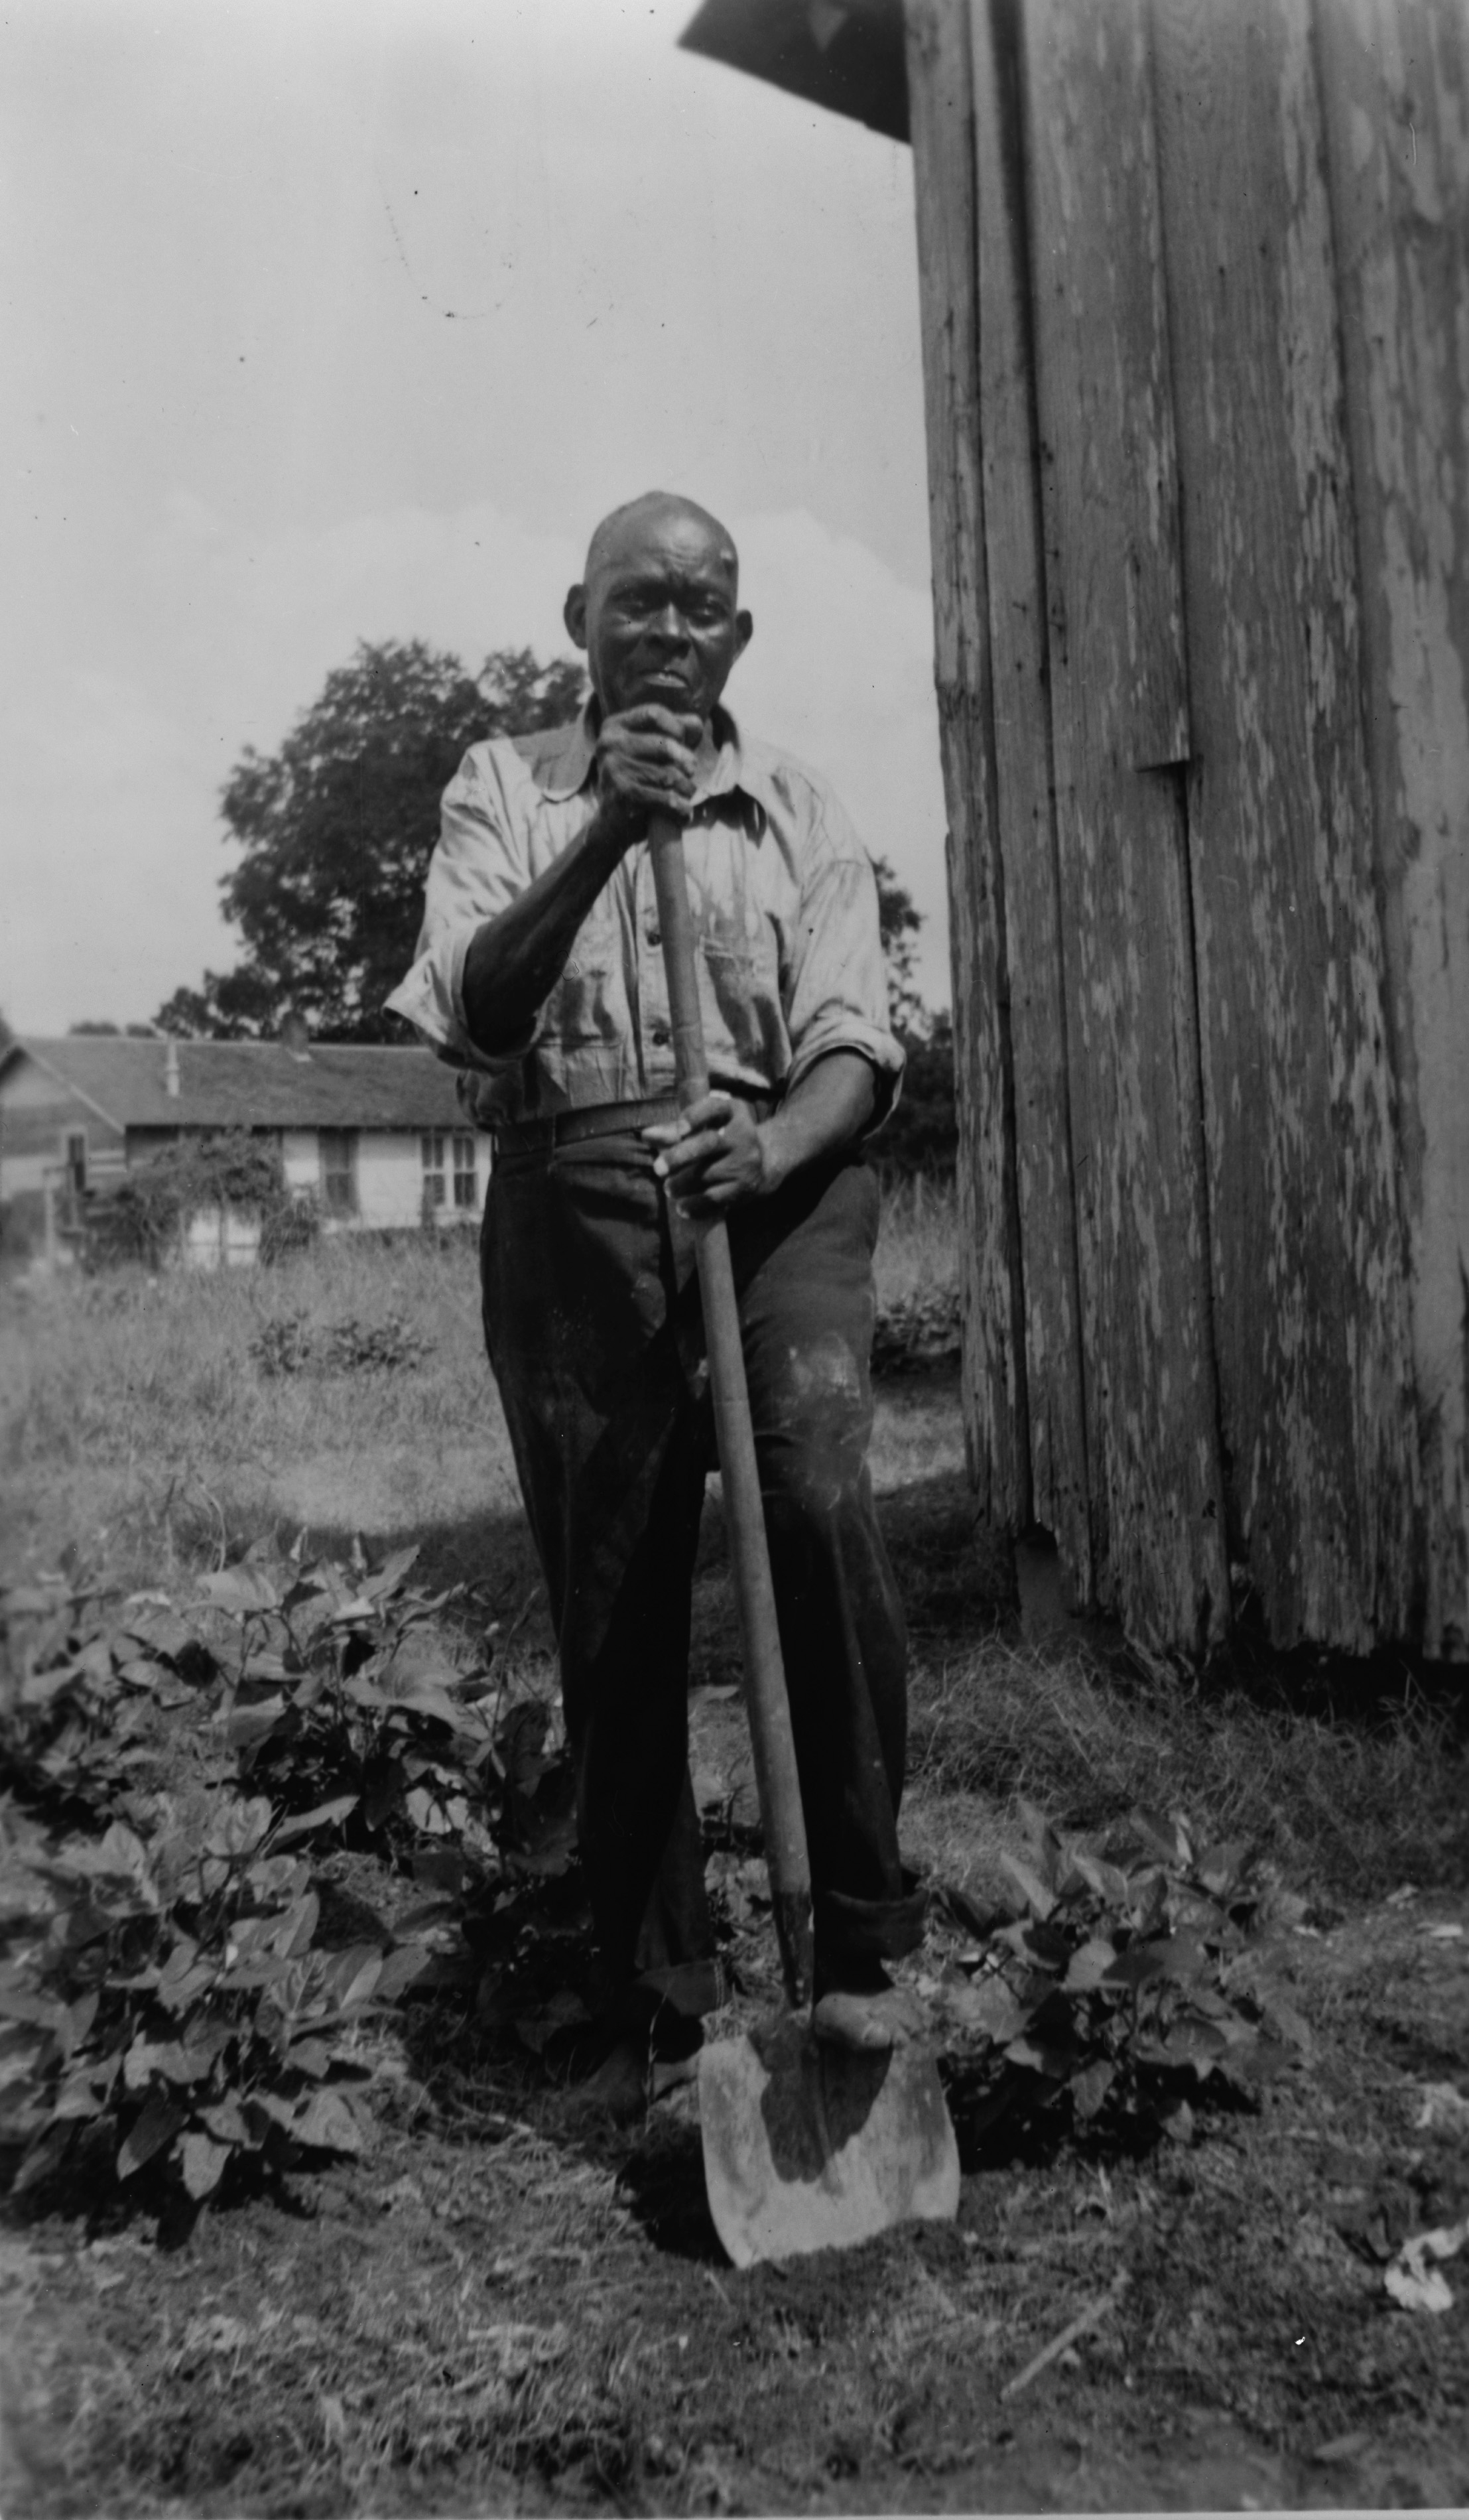
\includegraphics[width=90mm]{./imgs/geosimmons_recorte.jpg} \label{img5}
\caption{George Simmons}
%\end{minipage}
\end{figure}

\subsection{Bryant Huff, narrativas da Geórgia, Parte \versal{II}, página 240}
\label{ref151}

``A alimentação era fornecida pelo senhor, que a distribuía em rações
semanais regulares. Couve, ervilha, carne defumada e pão de milho eram
os pratos principais em todos os cardápios. Aos domingos, era dada uma
pequena quantidade de farinha para biscoitos e um pouco de café;
leitelho sempre havia em abundância. Os feriados quase sempre
significavam churrascos, com o abate de grandes porcos e vacas e uma
grande quantidade de carne fresca era dada a cada pessoa. Como todos os
alimentos eram cultivados na fazenda, todos tinham bastante''.

\subsection{George Simmons, narrativas do Texas, Parte \versal{IV}, página 24}
\label{ref239}

``O senhor Jaynes deixava os escravos que queriam plantar uma hortinha,
com legumes e coisas assim. Ele dava a semente e o negro podia ficar com
tudo que nascesse na sua roça. A gente era tudo bem cuidado e não sei no
que a liberdade foi tão melhor. É claro que alguns senhores eram ruins
para os seus escravos e açoitavam eles tanto que quase morriam. Eu sei
disso, porque ouvi dizer das fazendas vizinhas''.

\subsection{Annie Row, narrativas do Texas, Parte \versal{III}, página 258}
\label{ref229}

``A comida era quase sempre farinha de milho e melaço e carne, que era
pesada e tinha que durar por toda a semana. A verdade é que várias vezes
a gente passava fome. Tudo que se vestia e comia era criado na fazenda,
exceto sal, pimenta e coisas assim. Eles plantavam o algodão e o trigo,
o milho e a cana, além de frutas e coisas assim, e também galinhas,
ovelhas, vacas e porcos''.

\subsection{Campbell Armstrong, narrativas do Arkansas, Parte~I,~página~69} \label{ref10}

``Eles pesavam as coisas e davam para você e melhor não voltar depois.
Eles davam 1,3 quilos de carne, um quilo de farinha e um litro de melaço,
quando faziam. Às vezes, tinham a ideia de dar farinha ou algo assim.
Mas você tinha que aceitar o que davam. Eles davam as rações todos os
sábados, para durar a semana''.

\subsection{Oliver Bell, narrativas do Alabama, página 28} \label{ref24}

``Não, não era tão ruim assim com a gente. Os brancos eram bons para os
negros. A gente tinha o que chega de comer, verduras e tal, da casa
grande. As nossas rações eram pesadas; um celamim de farinha, 1,3 quilos de
carne, dois litros de melaço, feito em casa em moinho de madeira, e isso
era tudo para uma semana. Às vezes, aos domingos a gente ganhava um
pouco de açúcar, café e farinha. Não, senhora, a gente não sabia o que
era arroz.

O que eu vi da escravidão era uma má ideia, acho, mas todo mundo achava
que o seu senhor era o melhor do mundo. Ninguém sabia de nada. Os homens
ficavam verdinhos antes de descobrir que o mundo inteiro não pertencia
ao seu velho senhor''.

\subsection{Anne Maddox, narrativas do Alabama, página 273}
\label{ref179}

``Lá pelas quatro da tarde, todos os negrinhos eram chamados para o
pátio grande, onde a cozinheira colocava o leite em um cocho de madeira
comprida e esfarelava fogaça nele. A gente também tinha caldo de
vegetais no cocho também. A gente comia o pão e tomava o leite com
conchas e tinha que usar nossas mãos, mas era gostoso''.

\subsection{John Eubanks, narrativas do Indiana, página 73} \label{ref83}

```Eu lembro bem de quando a gente era pequeno na plantação dos
Everett', ele conta. `Eu trabalho desde que consigo me lembrar,
capinando, apanhando algodão e fazendo outras tarefas pela fazenda. A
gente não tinha muito o que vestir, nunca roupa de baixo, nada de
sapato, só um macacão velho e uma camiseta esfarrapada, no inverno e no
verão. Quando chegava o inverno, era tão frio que meus pés ficavam
dormentes quase todo o tempo. Várias vezes, quando dava, a gente
expulsava os porcos e colocava nossos pés na lama que eles tinham
esquentado. Os pés rachavam e a pele na sola e nos dedos rachava e
sangrava quase que o tempo todo, com umas cascas de sangue, mas no verão
ela se curava'".

\subsection{Isaam Morgan, narrativas do Alabama, página 282}
\label{ref200}

``Nós vivíamos bem como você imagina. Tinha a nossa senzala normal,
cabanas de madeira branca com barro nas frestas, e os escravos tinham
construído camas e uma lareira aberta bem grande onde cozinhavam. Sempre
tinha bastante o que comer. Era só pedir e o senhor fazia o resto. A
nossa ração era distribuída todos os domingos. Uma das melhores comidas
da minha vida foi gambá com batata. A gente saía de noite com um sacão e
uma matilha e não demorava nada para achar um gambá e acuar ele em uma
árvore. Quando isso acontecia, os cachorros ficavam latindo em volta da
árvore. Se a árvore era pequena, a gente podia sacudir o gambá. Se era
grande, um dos negros tinha que escalar e pegar o Sr. Gambá ele mesmo''.

\subsection{Jerry Hill, narrativas da Carolina do Sul, Parte~\versal{II},~página~289}
\label{ref145}

``Ele diz que sempre teve bastante comida; no entanto, a maioria dos
`crioulos' tinha que comer fogaça {[}\emph{ash"-bread}{]}, que é pão de milho
assado em cinzas quentes raspadas da lareira. Ele recebia biscoitos uma
vez por semana, mas estes representavam um luxo para as pessoas de cor.
Ele conta que quando um escravo precisava ser açoitado, ele era levado
para um pelourinho em Jonesville. Um relho era usado para o castigo e
arrancava sangue das costas nuas do homem ou mulher sendo açoitado. Um
dia, um escravo adulto recebeu 150 chibatadas por ensinar jogos de azar
aos meninos. Ele assistiu à aplicação desse castigo''.

\subsection{Thomas Anderson Carlisle, narrativas da Carolina~do~Sul,~Parte~II,~página~56}

``Tinha um dia especial em cada fazenda em que o senhor e o feitor
distribuíam a ração de cada semana. Era assim: dois quilos de toicinho,
um celamim de farinha de milho, um quilo de farinha e um litro de melaço
do negro, e essa era ração para toda a semana. Tinha um cepo enorme onde
toda a carne era cortada. Naqueles tempos, toda a carne vinha da
fazenda, dos porcos do senhor. Pedacinhos de carne ficavam presos nas
ranhuras desse cepo. O machado de carne era largo e pesado. A ração
pesada chegava na sexta"-feira. No sábado, vinha o ombro de porco para o
desjejum de domingo, e a farinha vinha no sábado também. Nosso senhor
nos dava canjica para o desjejum de domingo para quando a gente tinha
carne vermelha com caldo''.

\subsection{John Williams, narrativas do Arkansas, Parte~\versal{VII},~página~173}
\label{ref291}

``Quem ficava na casa dos brancos comia bem, mas quem ficava no eito
eles alimentavam quase como se daria comida para os porcos. Eles tinham
essas gamelinhas de madeira onde colocavam um pouco de carne gorda,
caldo de vegetais e pão de milho, e também canjica e coisas assim. Os
biscoitos vinham só no domingo.

Algumas velhas cozinhavam para as crianças escravas e outras para os
peões. Quem estava na casa grande ficava na casa grande''.

\subsection{Addie Vinson, narrativas da Geórgia, Parte~\versal{IV},~páginas~108--09}
\label{ref266}

``Domingo era dia de folga para todos os escravos na nossa fazenda. É
óbvio que os homens tinham que cuidar dos bichos no terreno logo atrás
das cabanas. As mulheres cozinhavam o dia inteiro para a próxima semana.
Se eles tinham a ideia de ir à igreja, prendiam as mulas a umas carroças
parecidas com conchas de servir e nos levavam sacudindo estrada abaixo.
No Natal, nos davam quatro dias de folga. A velha senhora nos dava muita
coisa boa para comer naqueles quatro dias; tinha bolo, carne fresca e
várias frutas secas que ficavam guardadas. (\ldots{}) No Dia de Ano
Novo, se não tinha nevado demais, os negros tocavam fogo nas moitas e
desmatavam mais terreno''.

\subsection{Tempie Cummins, narrativas do Texas, Parte I, página 266} \label{ref64}

``Eu nasci na fazenda do velho Foley, no Condado de Lavaca {[}Texas{]}.
Ele tinha mais de 100 escravos. Ele sempre comprava escravos, nunca
vendia. Quantos hectares de terra ele tinha? Meu Deus, aquele homem não
tinha hectares, tinha léguas. Ele plantava algodão e milho e criava gado
e porcos. A fazenda do velho Foley se espalhava pelos dois condados,
Lavaca e Colorado, ele tinha 650 hectares em um bloco e parte no rio
Navidad. O velho Foley morava em um casarão de madeira com dois quartos
duplos e um salão, e construiu uma tecelagem encostada na casa dele e
depois outra casa para as rodas de fiar. E o velho Foley também tinha o
seu próprio descaroçador de algodão e o seu próprio moinho onde moíam o
milho, e também tinha uma baita plantação de batata.

Era uma gente dura e tratavam todo mundo com dureza. Nós morávamos na
senzala, as casinhas todas bem apertadinhas, mas dava para caminhar
entre elas. Todas as cabanas tinham um quarto só, e quase sempre duas
famílias moravam juntas naquele quarto com chão de terra. Os escravos
construíam as cabanas, eles não ganhavam dinheiro e não ganhavam
terra''.

\subsection{Sarah Wilson, narrativas do Oklahoma, página 345}
\label{ref300}

``Os negros moravam todos amontados em cabaninhas de um quarto só, com
chaminés de barro e galhos. Nós morávamos em uma, com camas para as
crianças que pareciam prateleiras na parede. Mamãe costumava nos ajudar
a subir nelas''.

\subsection{Richard Carruthers, narrativas do Texas, página 197} \label{ref49}

``Naquele tempo, os chefes tinham casas boas, mas os negros tinham
cabanas de madeira e elas queimavam de vez em quando. A chaminé pegava
fogo porque era feita de galhos e barro e barba"-de"-velho. Muitas vezes a
gente precisou acordar de madrugada para empurrar a chaminé para longe
de casa, pois senão a casa pegava fogo.

As cadeiras eram quase todas tocos de madeira virados, ou lajes, bem
cruas, e as camas eram feitas que nem andaime. A gente fazia uma espécie
de colchão usando casca de milho ou barba"-de"-velho''.

\subsection{Alice Green, narrativas da Geórgia, Parte \versal{II}, página 40}
\label{ref108}

``Os escravos moravam em cabanas de madeira rebocadas a barro, com
chaminés feitas de galhos e lama. Meu Deus do Céu! Aquelas camas eram
feitas com umas vigas bem compridas e cordas entrelaçadas no lugar do
estrado de molas. Ninguém tinha mola de arame naquela época. Nossos
colchões eram de palha de trigo enfiadas em capas de tecido grosseiro
tecidos no tear lá mesmo na fazenda''.

\subsection{Yach Stingfellow, narrativas do Texas, Parte~\versal{IV},~página~69}
\label{ref255} 

``A gente cortava duas mudas de árvore do tamanho certo para amarrar na
ponta e enfiava nos buracos da parede para fazer a cama. Uma rede de
couro ou qualquer outro tipo de corda entre as varas seguravam a cama no
lugar. Depois a gente colocava feno ou palha de milho e um pouco de
algodão nas capas.

A gente comia toicinho, pão de milho e verduras, mas os brancos tinham
mais e melhor''.

\subsection{Spencer Barnett, narrativas do Arkansas, Parte~I,~página~117} \label{ref17}

``Os escravos na nossa fazenda tinham camas de palha de trigo. Os
brancos tinham camas finas de pena de ganso''.

\subsection{Rev. Wade Owens, narrativas do Alabama, página 306}
\label{ref206}

``Era uma cabana de toras de madeira, barro e galhos com folhas, e
chaminés de barro e piso de laje. As camas se encaixavam na parede com
pranchas nas laterais, dois postes com pranchas pregadas no alto,
parecendo mesas. Uma caixa servia de cômoda.

`Todas as fogaças eram assadas sobre folhas de álamo e castanheira
quando assavam batatas', conta Wade. `Nós acordávamos cedo de manhã para
lamber o mel das folhas, era o nosso doce de criança. A gente não tinha
nada de vestir, só os camisões, e tinha chapéus e chancas feitos em
casa, duros feito tijolo, com pontas de latão. Eu achava que eram as
coisas mais bonitas que já tinha visto na vida'".

\subsection{Henry Cheatam, narrativas do Alabama, página 66} \label{ref54}

``Nós morávamos em cabanas de madeira rebocadas com barro para não
deixar a chuva e o vento entrar, e as chaminés eram feitas de barro e de
galhos. As camas eram feitas em casa e pregadas na parede com as pernas
no outro lado. A casa do senhor também era feita de toras de madeira,
mas era muito maior do que as cabanas dos negros e ficava bem na frente
das nossas''.

\begin{figure}[]
%\begin{minipage}{0,4\textwidth}
\centering
 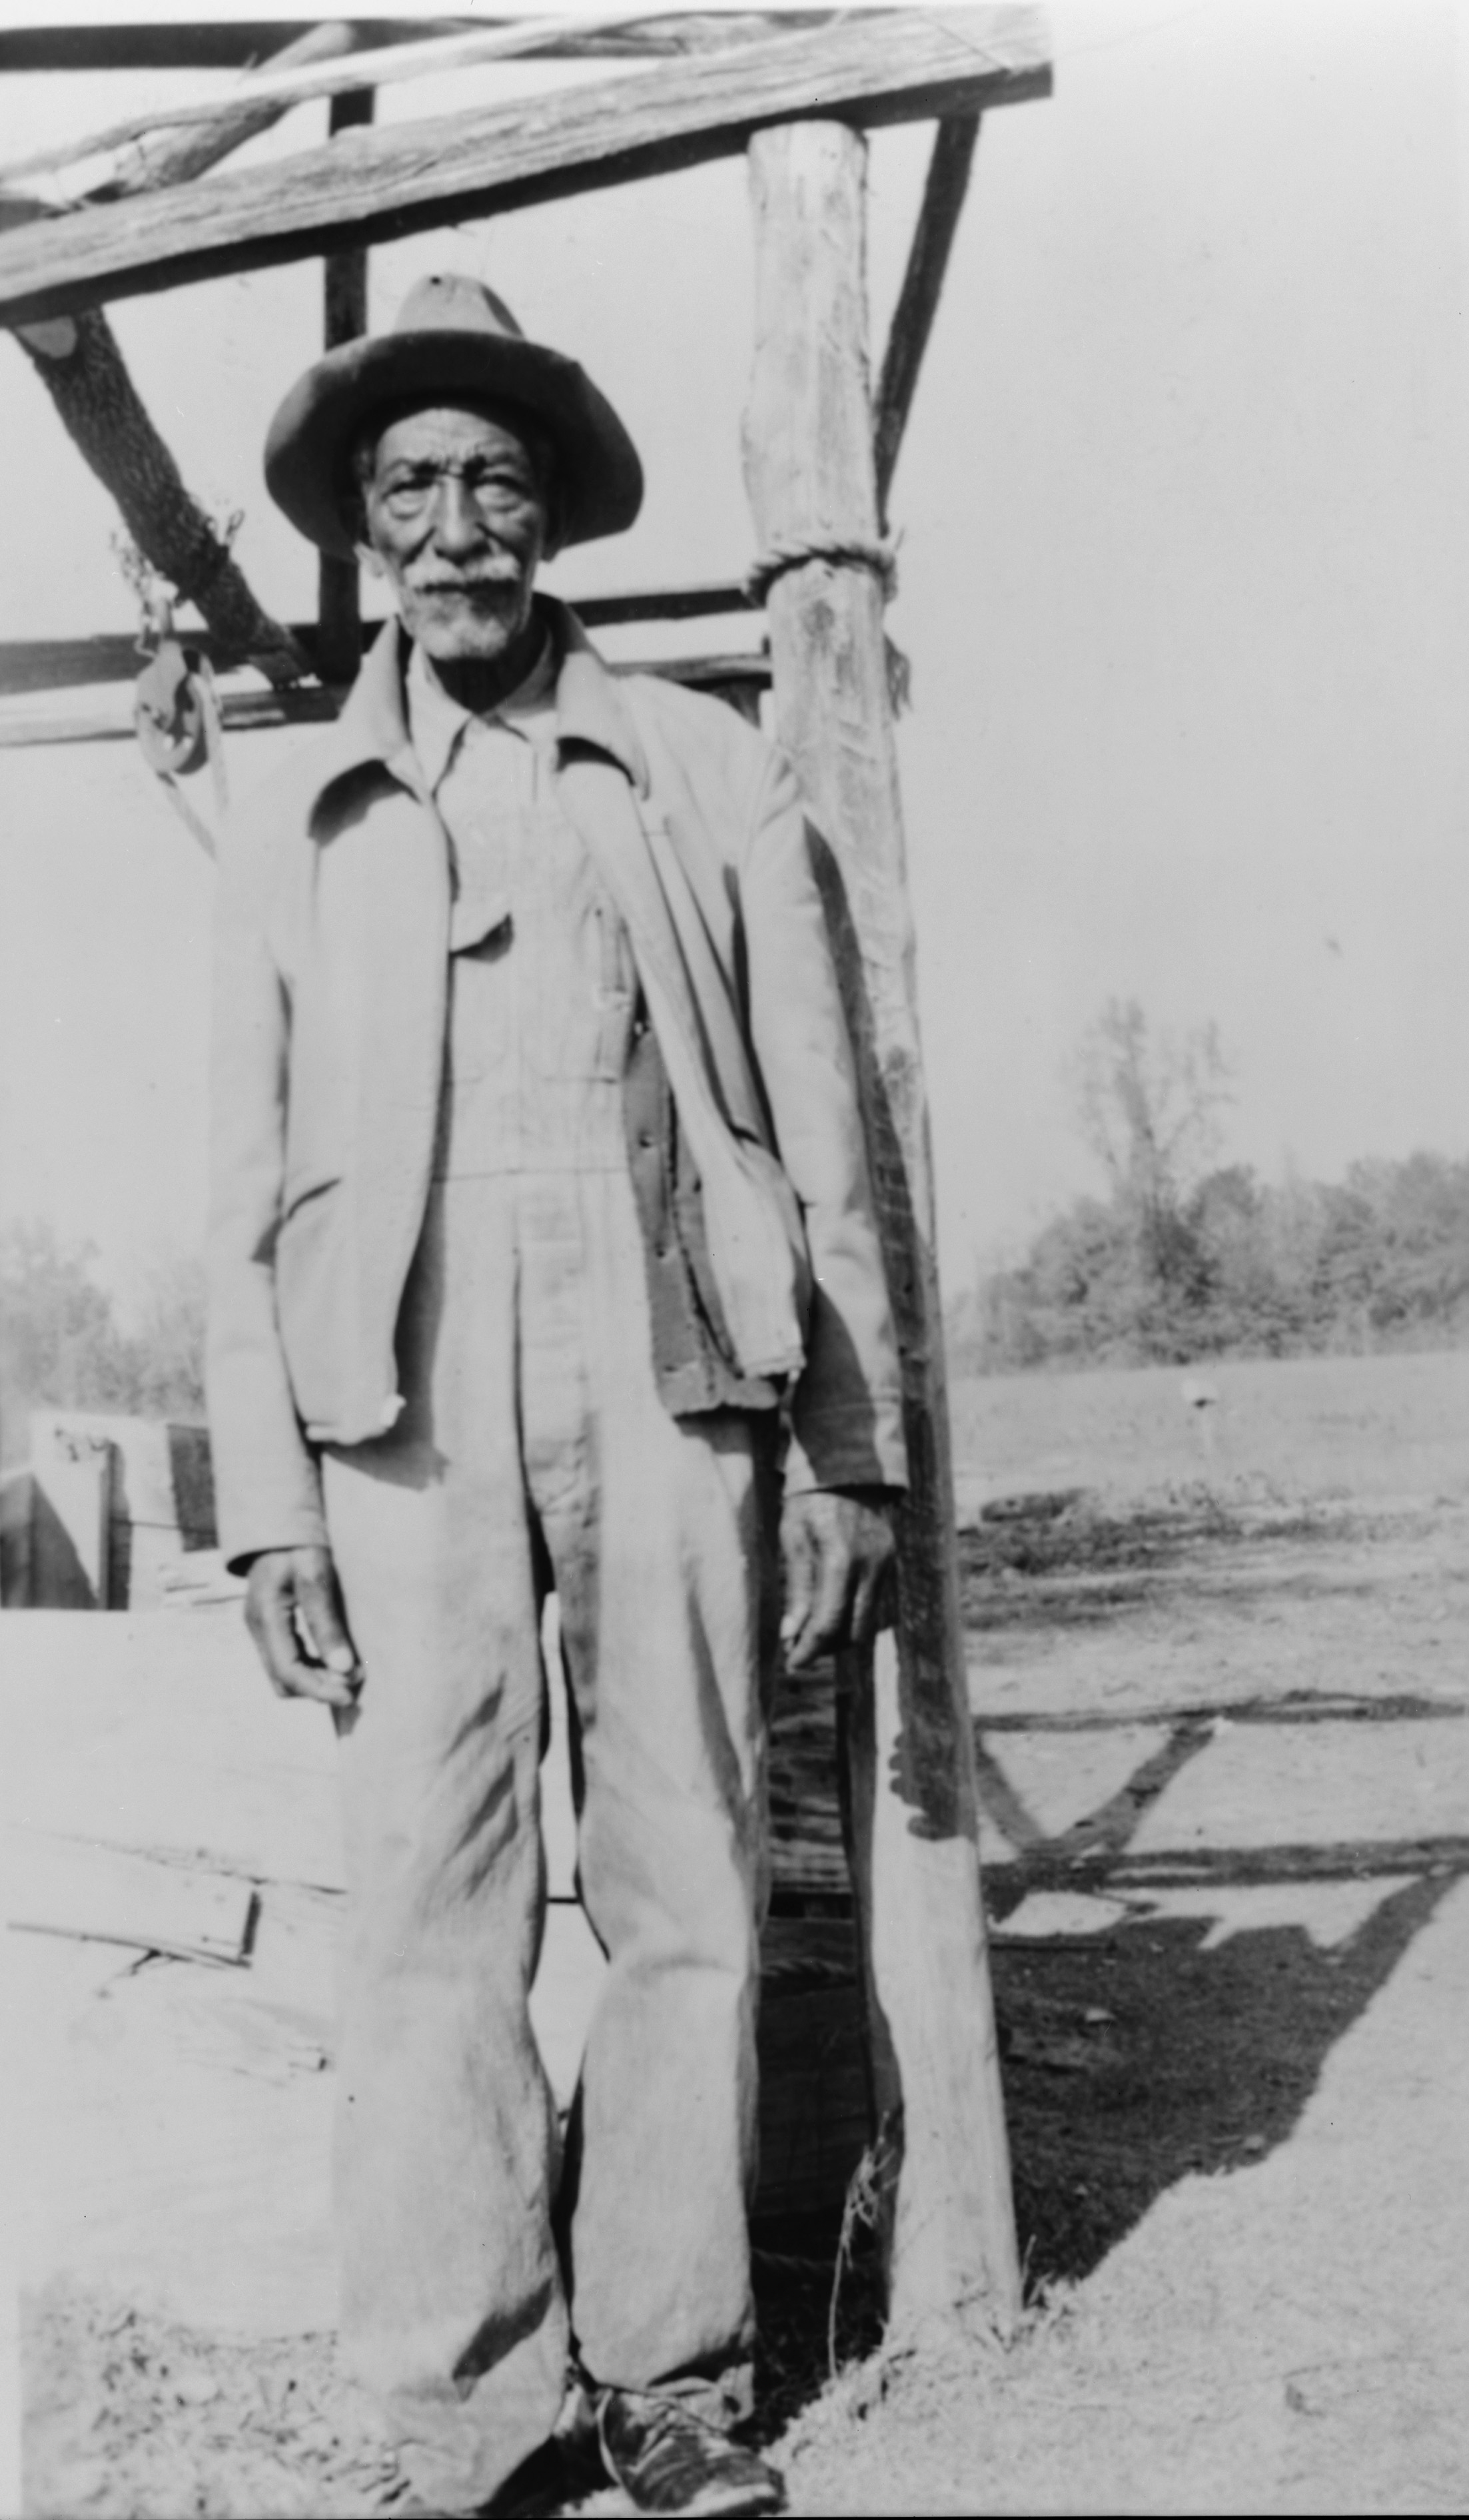
\includegraphics[width=90mm]{./imgs/campbelldavis_recorte.jpg} \label{img6}
\caption{Campbell Davis}
%\end{minipage}
\end{figure}	

\subsection{Campbell Davis, narrativas do Texas, Parte~I,~páginas~285--86} \label{ref68}

``Nos tempos da escravidão eu já era grande o suficiente para escutar
eles mandarem os negros acordarem de manhã e para ouvir os chicotes
assoviando e os cachorros latindo. Eu nasci no nordeste deste condado
aqui, bem na fronteira entre a Luisiana e o Texas, e pertencia ao velho
Henry Hood. Mamãe e papai eram Campbell e Judy Davis e os dois vieram do
Alabama, trazidos para cá pelos traficantes e vendidos para o senhor
Hood. Nós éramos nove filhos, nossos nomes eram Ellis e Hildaman e
Henderson e Henrietta e Georgia e Harriet e Patsy.

A casa do senhor Henry não era fina, mas era grande. A senzala ficava no
outro lado da plantação, na beira do mato. As cabanas tinham chão de
terra, uma lareira e camas velhas de poste e prancha pregadas nas
paredes.

De comer eles nos davam carne de gado e vegetais, qualquer tipo, tudo
que você imaginar, e nos deixavam passar o pão no caldo de legumes até
não poder mais. Era comida da boa e na minha vida toda eu nunca comi
melhor.

O senhor não deixava ter feitor na fazenda. Um dos meus tios era o
capataz, e o senhor soprava a concha velha bem antes do sol raiar. E se
os negros não saíam correndo, os chicotes estalavam.

Vi uma das minhas irmãs ser açoitada porque não tinha fiado o
suficiente. Puxaram as roupas dela até a cintura, deitaram ela de
barriga para baixo e chicotearam ela com o relho. Eu estava no eito
quando açoitaram o meu tio Lewis por não apanhar algodão suficiente. O
feitor tirou a roupa dele e fez ele deitar no chão. Ele não estava
amarrado, mas diz que ficou com medo de se mexer.

As mulheres tinham folga na tarde de sexta para lavar as roupas, e todos
os peões tinham o sábado. Quase todos os homens saíam para caçar ou
pescar. Às vezes, eles faziam uma festa no sábado de noite e os casais
dançavam ao som do banjo e da rabeca''.


\subsection{Lorenza Ezell, narrativas do Texas, Parte \versal{II}, página 25} \label{ref86}

``O velho Ned Lipscomb era um dos melhores senhores de todo o contado.
Os patrulheiros, sabe, eles nos chamavam de `crioulos livres do Velho
Ned', e nos odiavam. Eles eram cruéis com a gente, pois achavam que o
nosso senhor era bom demais. Uma vez, eles pegaram meu tio e quase
mataram a pancadas.

A gente ia trabalhar quando o sol nascia, mas não abusavam de nós. Os
outros senhores costumavam tocar a corneta ou o sino, mas o nosso nunca
usava nem a corneta nem o chicote. Todos os homens podiam cuidar de uma
roça com tabaco ou algodão para vender no mercado. Não tinha muitos
senhores que deixavam os seus negros terem roças, e alguns nem
alimentavam eles direito. É por isso que eles tinham que sair de noite
para arranjar comida, fosse como fosse''.

\begin{figure}[]
%\begin{minipage}{0,4\textwidth}
\centering
 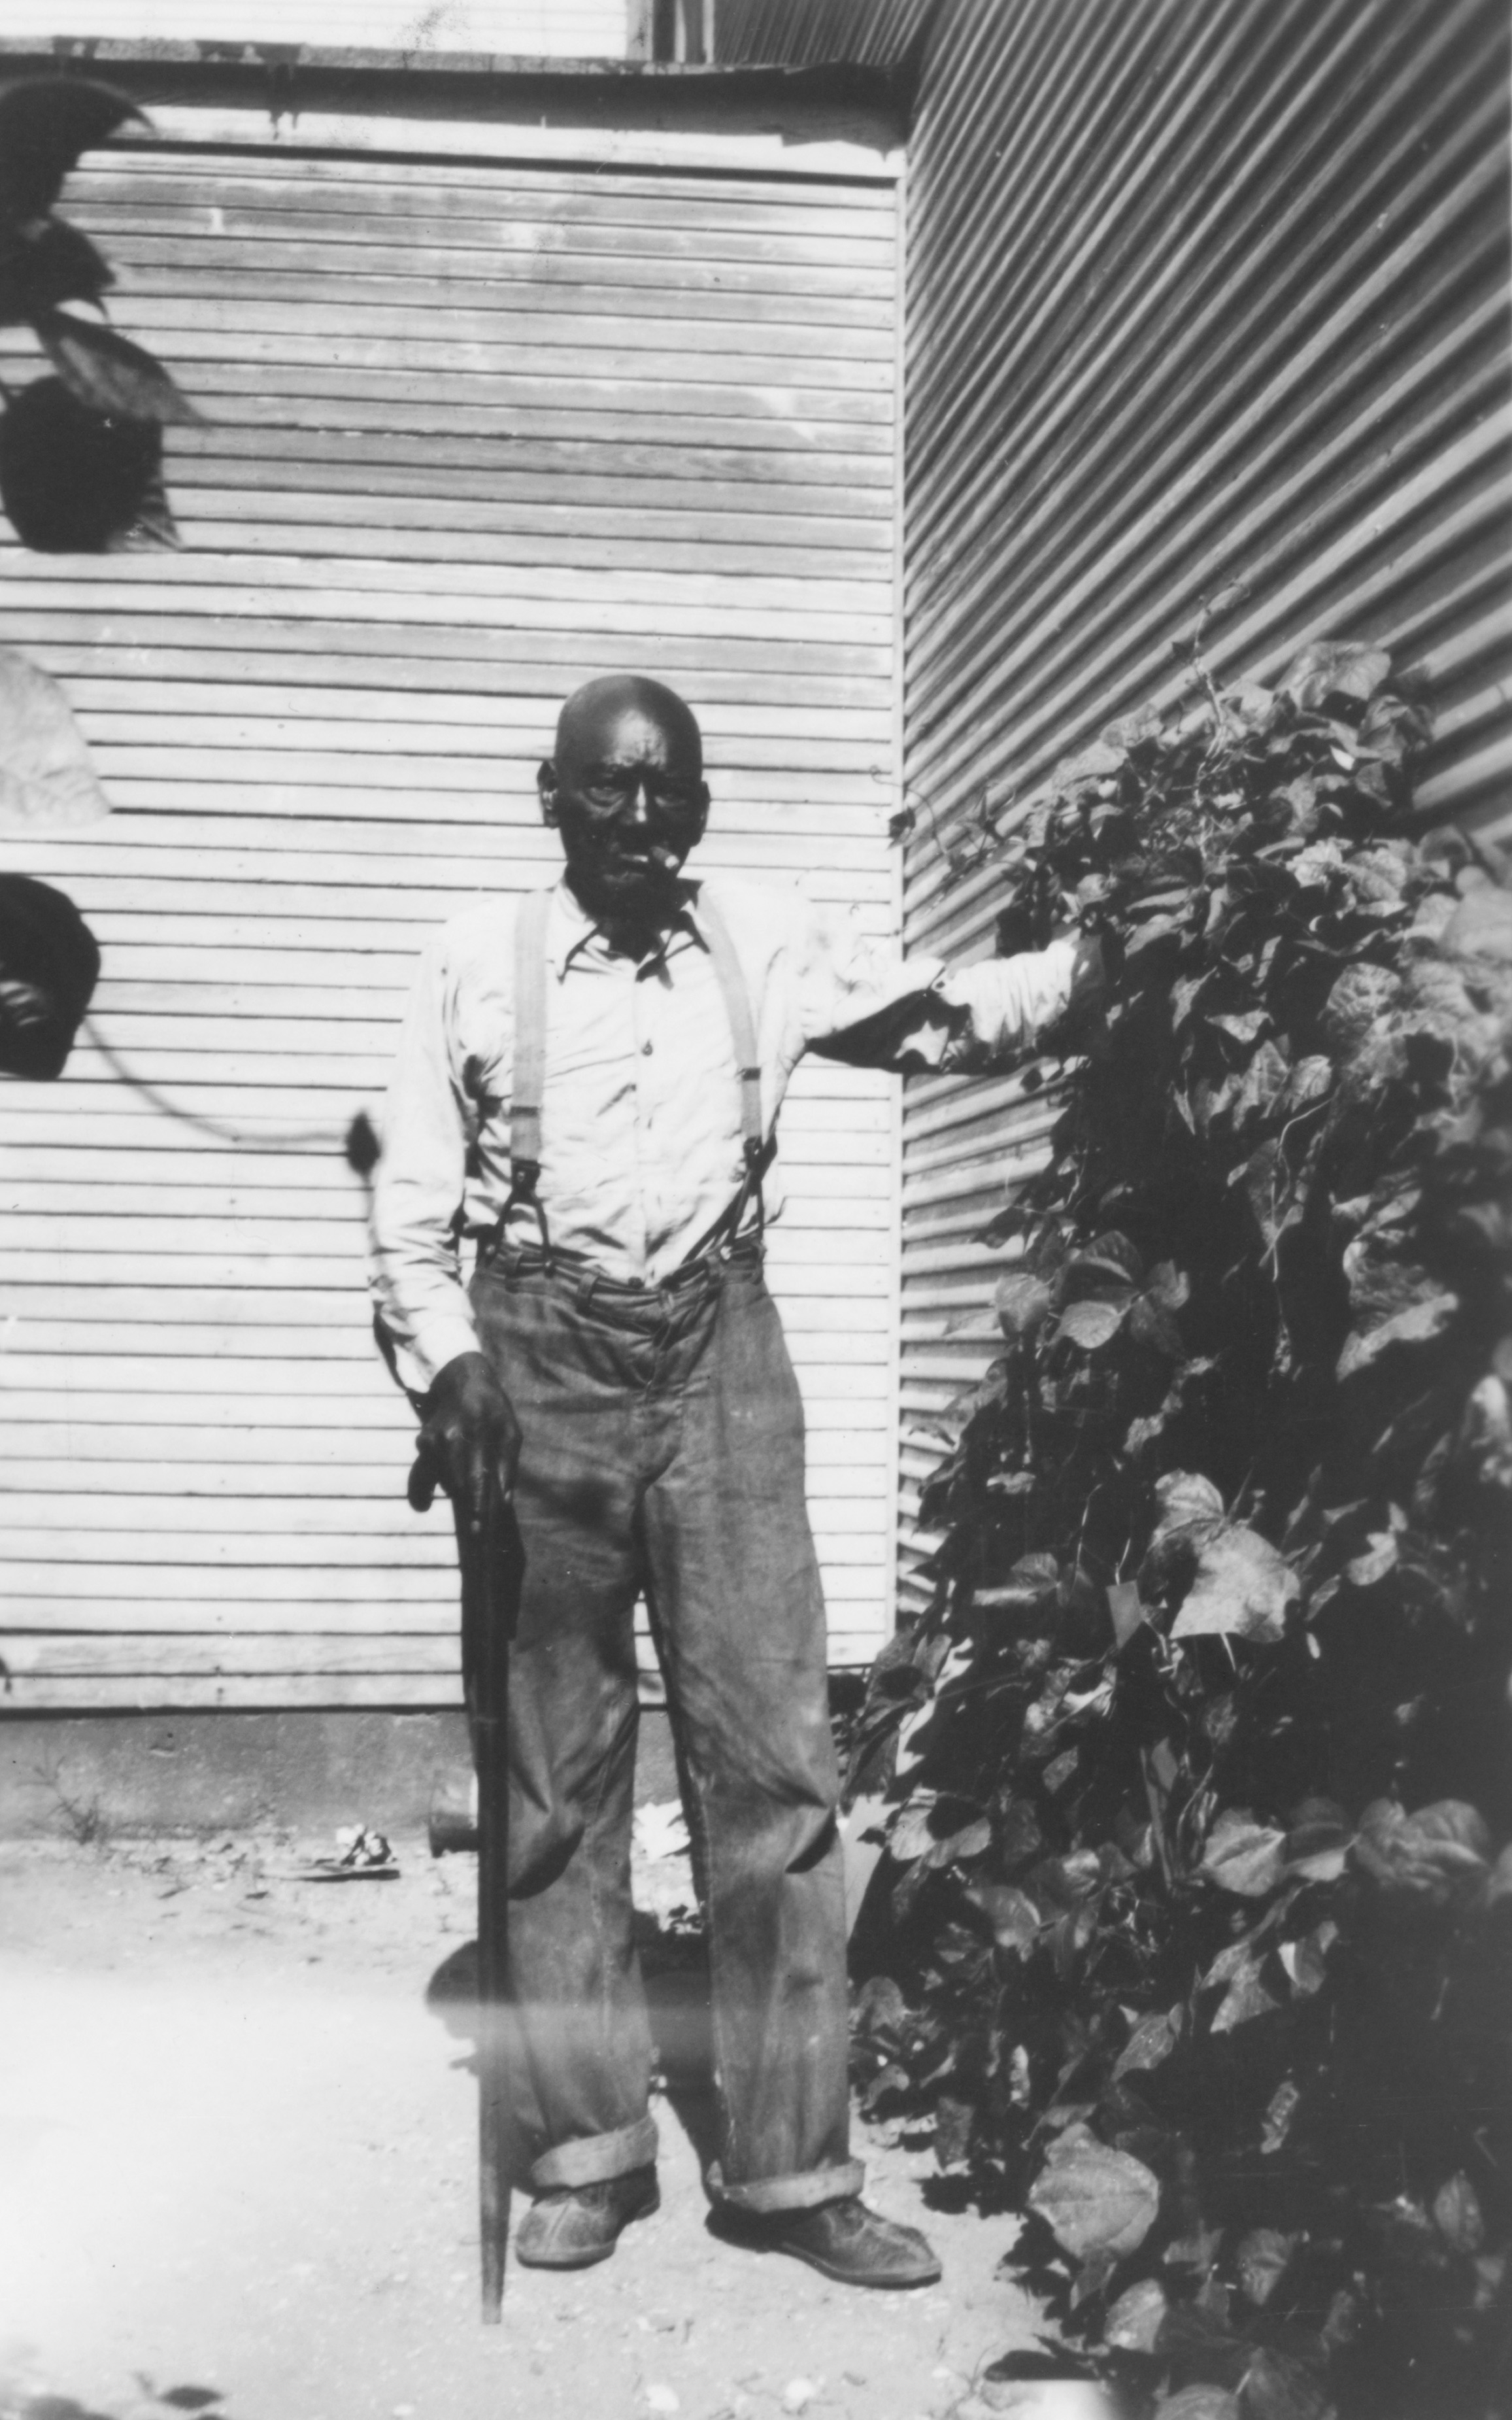
\includegraphics[width=90mm]{./imgs/lorenzaezzell_recorte.jpg} \label{img7}
\caption{Lorenza Ezell}
%\end{minipage}
\end{figure}

\subsection{Lewis Bonner, narrativas do Oklahoma, página 17} \label{ref28}

``Minha família e todos os escravos da nossa fazenda eram bem tratados,
quase não se açoitava naquelas bandas. O senhor era o feitor dos seus
negros e não usava mais ninguém. Eu servia a mesa e desnatava na casa
grande.

Eu comia à mesa com a minha senhora e a família e nunca ninguém disse
nada. A gente comia toicinho, verdura, batata irlandesa e isso que se
come agora. A Tia Chaddy era a cozinheira e ama de todas as crianças da
fazenda.

A gente ouvia os escravos das outras fazendas berrando com as
chicotadas, mas o nosso senhor nunca castigava os seus negros, exceto
quando mentiam. Às vezes, escravos das outras fazendas fugiam e se
escondiam na nossa. O senhor levava eles de volta e dizia para os donos
como deviam tratá"-los para eles não fugirem de novo''.

\subsection{Sam Jones Washington, narrativas do Texas, Parte~\versal{IV},~páginas~138--39}
\label{ref280}

``Uma noite o senhor disse: `Não amarra o meu cavalo no poste esta
noite', mas eu estava com sono, comecei a cabecear e peguei no sono.
Mamãe me sacudiu e disse: `Você prendeu o cavalo no poste?' O senhor viu
o cavalo de manhã e disse: `Você prendeu aquele cavalo quando eu mandei
não prender'. Ele me deu umas chicotadas e eu aprendi a fazer o que
mandavam. Ele nunca açoitava ninguém, não os castigos fortes que nem os
outros negros levavam. Ele era um bom senhor''.

\begin{figure}[]
%\begin{minipage}{0,4\textwidth}
\centering
 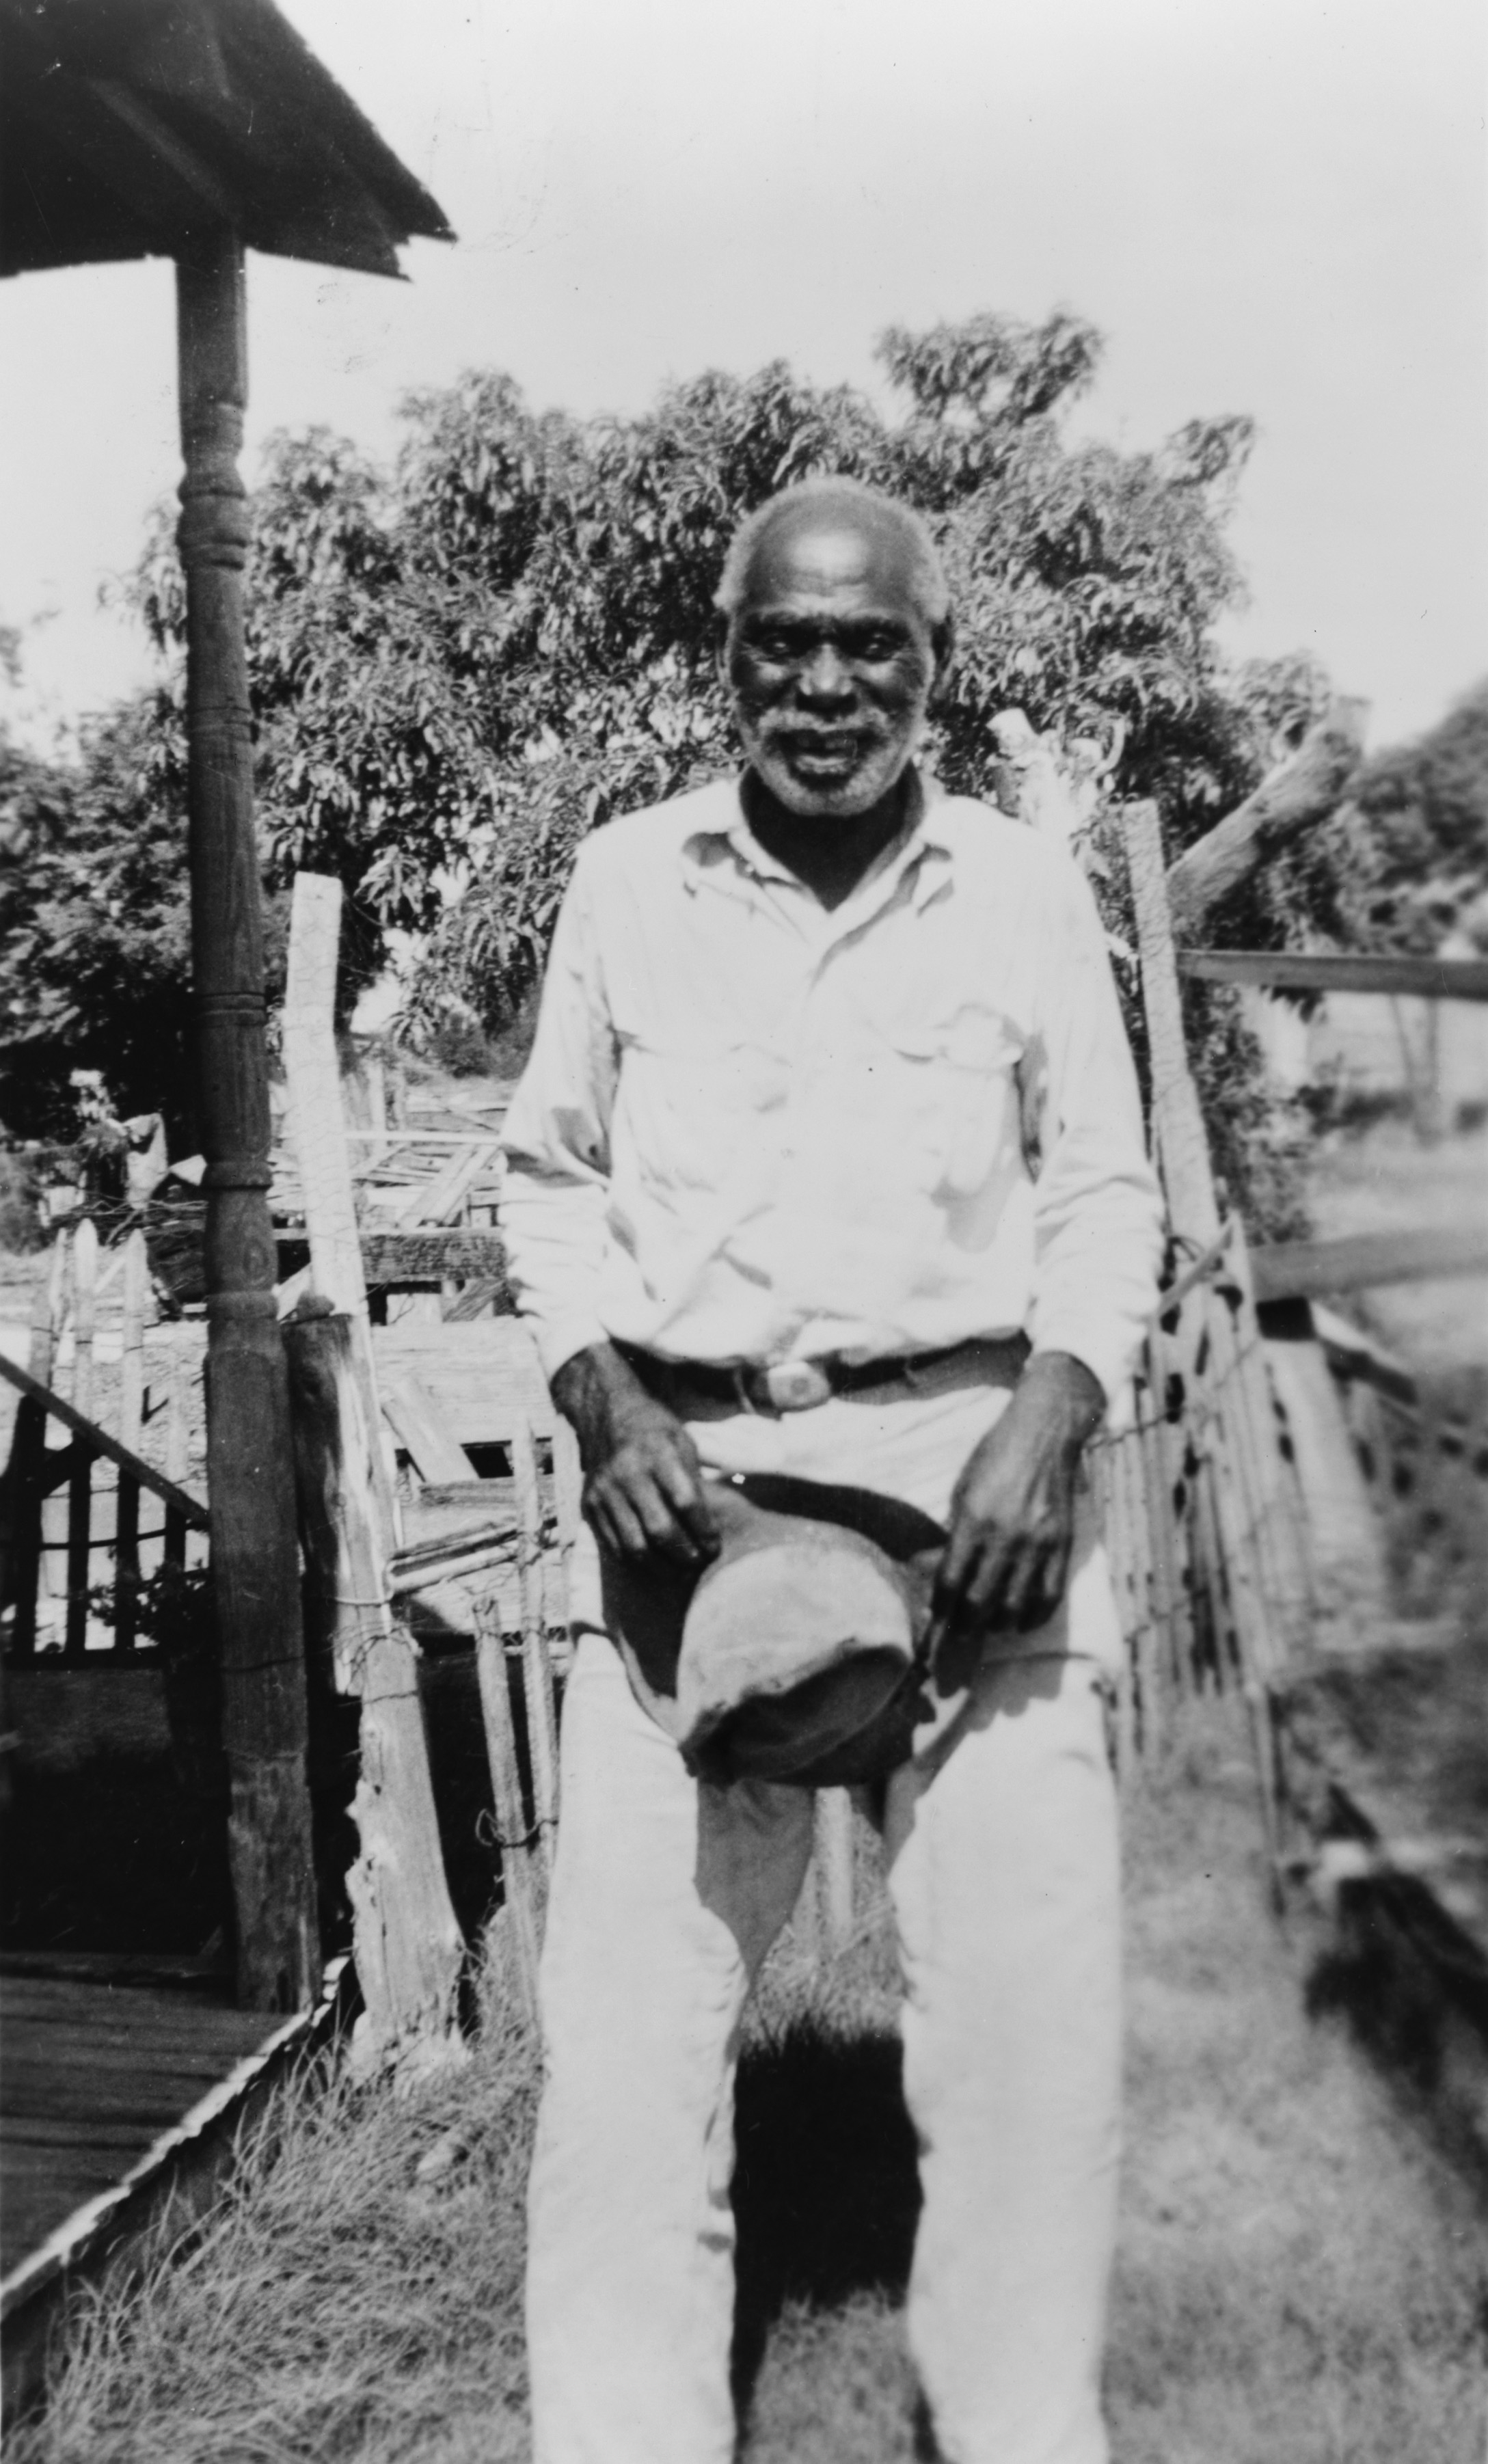
\includegraphics[width=90mm]{./imgs/samjones_recorte2.jpg} \label{img8}
\caption{Sam Jones Washington}
%\end{minipage}
\end{figure}

\subsection{Will Sheets, narrativas da Geórgia, Parte \versal{III}, página 240}
\label{ref237}

``O senhor Jeff era um homem bom, ele nunca açoitava nem batia nos seus
negros. Não, senhora, ninguém nunca foi surrado na fazenda do senhor
Jeff, não que eu saiba. Ele não tinha feitor. Não precisava, porque ele
não tinha tantos escravos que não pudesse ser o próprio feitor. O senhor
Jeff tinha só quatro homens e quatro mulheres de escravo, e ele e o
senhorzinho Johnny trabalhavam no eito junto com os negros. Eles iam para
o campo quando o dia nascia e voltavam no final da noite''.

\paragraph{Comentário}\quad
{\small
Entre os elementos que dificultavam a vida dos escravos estava o
medo constante dos patrulheiros, grupos de homens brancos que, por lei,
precisavam se alternar em cavalgadas noturnas pelas estradas para manter
os escravos confinados às suas fazendas e sob controle. Além da fome, o
trabalho árduo e a falta de roupas quentes aos quais eram sujeitados, os
escravos se queixavam de serem proibidos de aprender a ler e escrever e
da dificuldade de praticarem sua religião sozinhos.
}

\subsection{Richard Jackson, narrativas do Texas, Parte \versal{II}, página 196}
\label{ref162}

``Lembro de mamãe sempre dizendo que os negros tinham que rezar no mato
porque não podiam fazer algazarra perto de casa. Ela diz que se vestiam
e comiam bem, mas que o feitor fazia eles trabalharem tudo que dava. Eu
não era grande o suficiente para trabalhar no eito, mas lembro de ir até
o campo para levar o cachimbo para mamãe. Ninguém tinha fósforo naquela
época e eu sempre levava o fogo de casa e acendia um cepo no campo para
que mamãe pudesse acender o cachimbo.

Nenhum dos nossos pais aprendeu a ler e a escrever até depois da
escravidão. Meu irmão mais velho estava aprendendo a ler e a escrever às
escondidas, mas o feitor descobriu e acabou com isso. Ele descobriu umas
letras escritas com carvão na parede da senzala e fez os negros contarem
quem tinha escrito. Foi o Jack, meu irmão. O feitor não açoitou ele, mas
disse que era melhor não fazer mais aquilo''.

\subsection{Sylvia Cannon, narrativas da Carolina do Sul, Parte~I,~página~192} \label{ref45}

``Os brancos nunca ajudaram nenhum de nós dos negros a ler e escrever,
nunca. Eles ensinavam as crianças mulatas, mas se pegavam as negras com
um livro, quase nos matavam. Eles davam bem mais carinhos para os
mulatinhos do que para os negrinhos na fazenda. Mulheres do Norte foram
para lá depois da guerra, mas não deixaram elas ensinarem nada para
ninguém''.

\subsection{Dellie Lewis, narrativas do Alabama, página 257}
\label{ref170}

``Os escravos domésticos como nós, esses os brancos nos ensinaram a ler.
A minha vó, Alvain Hunter, que não tinha nada de educação, mas que sabia
a Bíblia de trás para a frente, ela nos fez estudar''.

\subsection{Eli Davison, narrativas do Texas, Parte I, página 296} \label{ref69}

``O senhor Will era mais um homem bom lá na Virgínia. Ele nunca ficava
brabo nem açoitava os escravos. Sempre tinha bastante de comer, com 500
hectares, mas quando a gente veio para cá, tudo que tinha para comer era
pão de milho e o que a gente matava no mato. Ele plantava três hectares
de milho, mas tudo que fazia era caçar veados e esquilos. Nunca um negro
tentou fugir do Texas, porque era uma boa terra, com bastante para comer
e para caçar, e não tão frio como na Virgínia.

Depois que eu fui vendido, meu novo senhor não era tão bom comigo. Ele
sempre achou que o Sul ia vencer a guerra e nos tratava com maldade. O
nome dele era Thomas Greer. Ele vivia dizendo que os crioulos nunca iam
ser livres. Quando ela chegou, ele nos disse: `Ora, seus negros ***,
vocês são livres como eu'. Ele nos soltou sem nada de comer e quase sem
roupas. Ele disse que se acordasse amanhã e visse um negro na fazenda,
ia descer o chicote em quem encontrasse''.

\subsection{Margaret Hughes, narrativas da Carolina do Sul, Parte~\versal{II},~páginas~328--29}
\label{ref153}

``Por falar em patrulheiros, eu morria de medo deles. Era preciso ter um
passe do nosso senhor para ir de uma fazenda à outra, e se saíamos sem
um passe, os patrulheiros nos pegavam e nos açoitavam. Mas eu eles nunca
pegaram''.

\subsection{Lucy Gallman, narrativas da Carolina do Sul, Parte~\versal{II},~página~101}
\label{ref98}

``Os patrulheiros lá onde a gente morava eram George Harris, Lamb Crew,
Jim Jones e Theodore Merchant. Eles nos incomodavam muito. No primeiro
dia do mês, alguém era colocado no pelourinho e surrado com uma pá de
carvalho, com furos para fazer bolhas, e então as bolhas se abriam com o
chicote de couro''.

\subsection{Alice Douglass, narrativas do Oklahoma, página 74} \label{ref73}

``Eu não tenho educação nenhuma. Naqueles tempos, era melhor nunca ser
pego com um jornal, pois se não você levava uma surra e quase cortavam
as suas costas fora. Quando os negros se libertaram, os brancos mataram
eles de encher carroças, pois disseram que era um levante dos negros. Eu
costumava me deitar no chão com os brancos e ouvir eles passarem. Os
patrulheiros andavam por todos os lados, tentando pegar negros sem
passes para dar uma sova neles''.

\subsection{Eliza Washington, narrativas do Arkansas, Parte~\versal{VII},~página~52}
\label{ref278}

``A melhor época que eu lembro na fazenda era quando se debulhava milho.
Traziam um monte de milho dos silos e espalhavam por onde todo mundo
podia pegar livremente. Depois, todos pegavam o milho e debulhavam até
ser hora de parar. Sempre se debulhava o milho à noite, e só se trazia
dos silos o quanto achavam que daria para debulhar. Logo antes de
terminar, eles começavam a cantar. Algumas das canções eram tão tristes,
davam tanta pena. Não lembro de nenhuma, mas ainda lembro que eram
tristes. Uma começava assim: `O especulador comprou minha mulher e meu
filho/ E levou embora'. Quando terminavam de debulhar, eles saíam à
caça do feitor, que fugia e se escondia logo antes. Se achavam ele, dois
homenzarrões botavam ele nos ombros e carregavam por todo o pátio
enquanto cantavam. Minha mãe me contou que costumavam fazer isso nos
tempos da escravidão''.

\subsection{James Hayes, narrativas do Texas, Parte \versal{II}, página 129} \label{ref129}

``Sabe, acho que eu era mais contente quando era escravo. Sempre fui bem
tratado e nunca me preocupei com como ia ganhar a vida. Desde que me
tornei livre, eu tive vezes em que fiquei cheio de preocupações. É claro
que não quero voltar para a escravidão, mas eu paguei pela minha
liberdade''.

\pagebreak
\thispagestyle{empty}
\movetoevenpage
\thispagestyle{empty}
\begin{absolutelynopagebreak}
\begin{vplace}
\begin{figure}[H]
\begin{adjustwidth}{-1.6cm}{}
  %\centering
  \vspace*{-2cm}
  %\hspace{-0.5cm}
  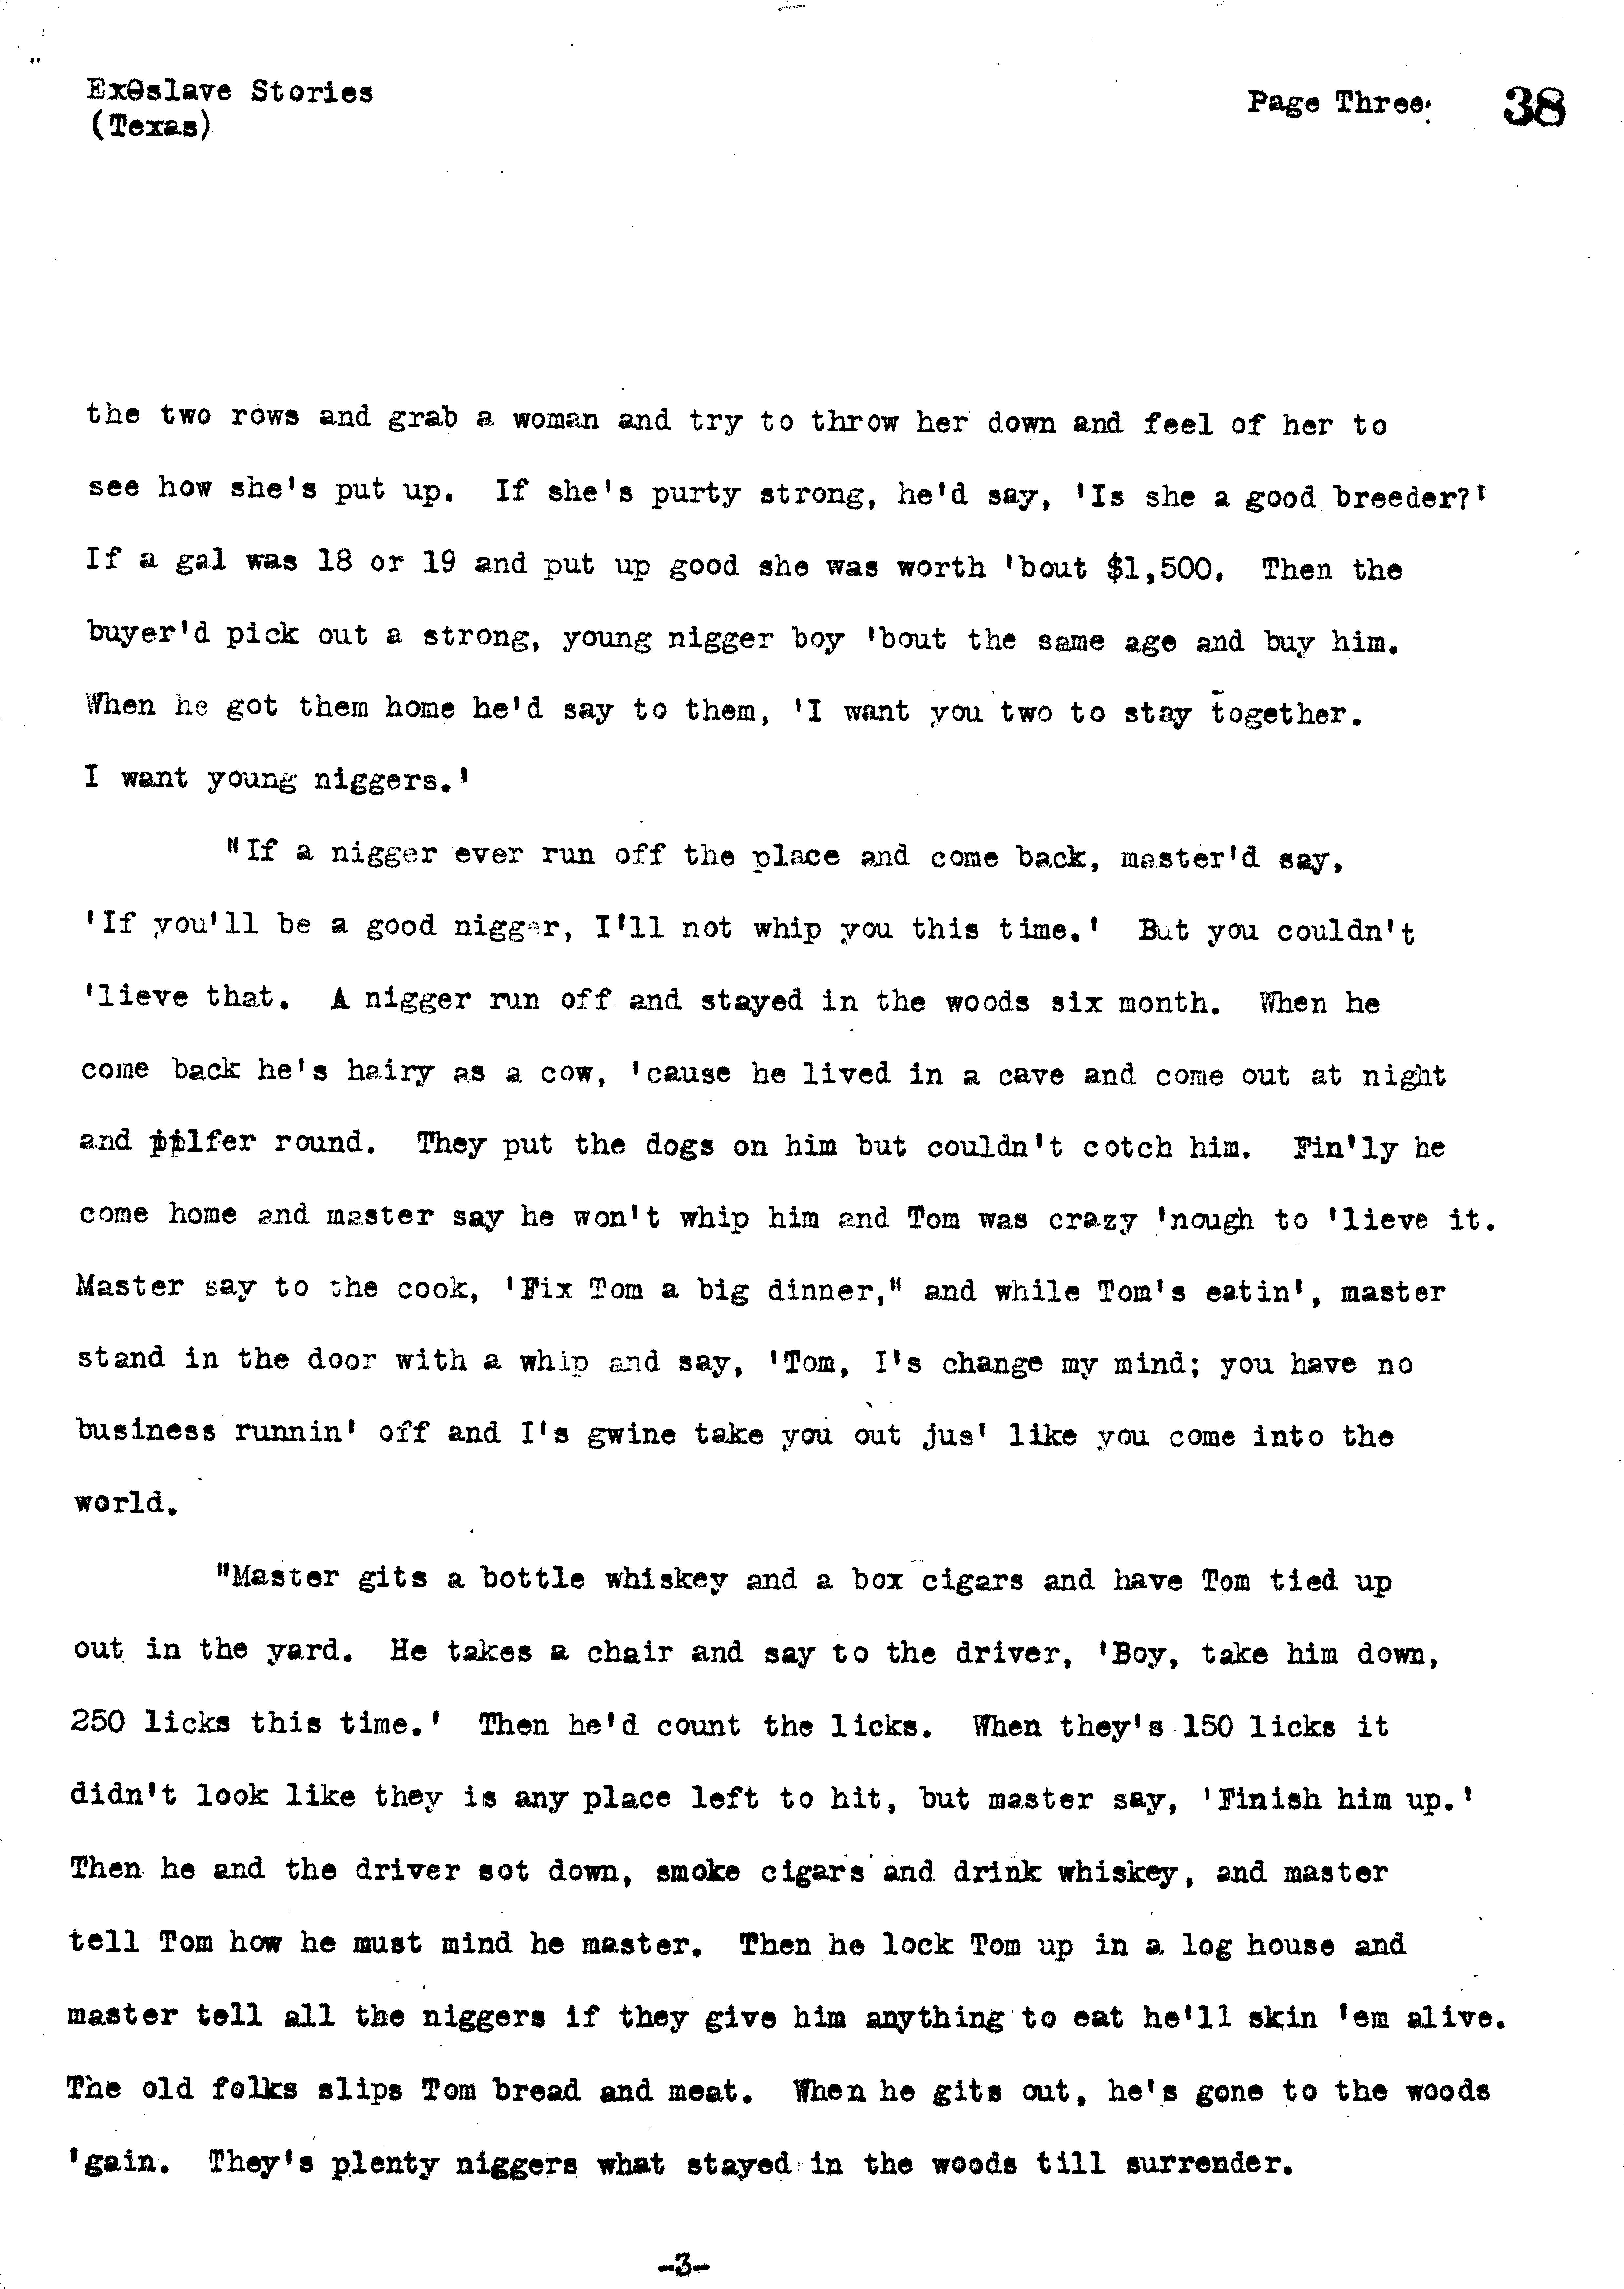
\includegraphics[width=130mm]{./imgs/Cap3.jpg}  
  %\hfill
\end{adjustwidth}
  \caption{Jordon Smith, narrativas do Texas, Parte \versal{IV}, página 38}
\end{figure}
\end{vplace}

\end{absolutelynopagebreak}

\chapter{Crueldade e castigos físicos}
%\addcontentsline{toc}{chapter}{{\large\versal{III.}} Crueldade e castigos físicos}
%\hedramarkboth{Crueldade e castigos físicos}{}

\subsection{Jordon Smith, narrativas do Texas, Parte \versal{IV}, páginas 38--39}
\label{ref245}

``Se um negro fugia e depois voltava, o senhor dizia: `Se for um bom
crioulo, eu não vou açoitar você desta vez'. Mas não dava para acreditar
nisso. Um negro fugiu e ficou no mato seis meses. Quando voltou, ele
estava peludo feito uma vaca, porque morava em uma caverna e saía de
noite para roubar umas coisinhas. Eles botaram os cachorros atrás dele,
mas não conseguiram pegar. Finalmente ele voltou para casa e o senhor
disse que não ia açoitar ele, e o Tom foi louco o suficiente para
acreditar. O senhor disse para a cozinheira, `faz um almoço bem grande
para o Tom', e enquanto Tom estava comendo, o senhor parou no lado da
porta com o chicote na mão e disse: `Tom, mudei de ideia, você não tinha
direito nenhum de fugir e vai aprender com a roupa que veio ao mundo'.

O senhor pegou uma garrafa de uísque e uma caixa de charutos e mandou
amarrarem o Tom no pátio. Ele puxou uma cadeira e disse para o feitor:
`Rapaz, dê um jeito nele, 250 chibatadas'. E então ele contou as
chibatadas. Quando chegou a 150 chibatadas parecia que não tinha mais
onde bater, mas o senhor disse `acaba com ele'. Depois ele e o feitor se
sentaram, fumaram charutos e beberam uísque e o senhor disse para o Tom
que ele tinha que ser obediente. Depois, ele prendeu o Tom em uma cabana
e disse para os negros que ia esfolar vivo quem desse alguma coisa de
comer para ele. Os velhos deram pão e carne às escondidas para o Tom.
Quando saiu de lá, ele fugiu para o mato de novo. Teve vários negros que
ficaram no mato até a rendição.

Ouvi alguns escravos dizerem que os brancos eram bons para eles, mas
onde a gente estava a briga era feia. Já pensei e repensei isso mil
vezes e decidi que é porque nem todos os homens são iguais. Alguns são
ruins e alguns são bons. É como é hoje em dia. Alguns chefes não têm
coração e alguns tratam você feito branco. Acho que sempre foi assim''.

\paragraph{Comentário}\quad
{\small
Um dos horrores, e um dos aspectos mais odiados da escravidão, era
o castigo físico. A escravidão se baseava fundamentalmente na coerção,
no uso de diversos métodos para forçar uma pessoa a se submeter à
vontade de outra. Os senhores insistiam que os escravizados deviam fazer
tudo que lhes mandassem, ou então seriam ``punidos''. Em 1829, a Suprema
Corte da Carolina do Norte reconheceu francamente o princípio desumano
por trás da escravidão: ``O poder do senhor deve ser absoluto para que a
submissão do escravo possa ser perfeita''.\footnote{State vs. Mann, 13
  North Carolina Reports, 263 (1829), Opinião de Thomas Ruffin.}
Os tribunais sulistas normalmente evitavam sancionar publicamente
um princípio de tamanha imoralidade, mas o sistema jurídico e a
sociedade escravista não impunham muitos limites ao que cada senhor de
escravos podia ou não fazer. A natureza extremamente rural de muitas
partes do Sul, e a ideia de que o fazendeiro controlava as suas
propriedades, ampliava ainda mais o escopo para crueldades.

A forma mais comum de ``castigo'' era ser açoitado, e as
narrativas dos escravizados estão repletas de descrições amargas e iradas
dessa prática. A análise quantitativa de todas as narrativas mostra que
o açoite, pelo menos de alguns trabalhadores, era comum nas fazendas, fossem
elas grandes ou pequenas, fosse o proprietário homem ou mulher. Mas
também existiam outras formas de coerção, e crueldades ainda mais
sádicas, como este capítulo irá mostrar.

Assim como em outros aspectos da escravidão, entretanto, muito
dependia da personalidade do senhor de escravos. Alguns indivíduos eram
profundamente religiosos ou compassivos, enquanto outros eram bêbados,
violentos ou pior. Naturalmente, os escravizados prestavam atenção a essas
diferenças.
}

\subsection{Claiborne Moss, narrativas do Arkansas, Parte~V,~páginas~155--57}
\label{ref203}

``Eu nasci no Condado de Washington, Geórgia, na fazenda de Archie
Duggins, a 25 quilômetros de Sandersville, a sede do condado, em 18 de
junho de 1857. (\ldots{})

Onde cresci, Duggins não era um homem malvado. Os escravos dele não
saíam para trabalhar até depois do sol nascer. O irmão dele, que morava
a cinco quilômetros da gente, fazia o seu pessoal acordar antes do sol.
Mas Duggins não fazia isso. Ele parecia ter alguma consideração pelos
seus. Todos os sábados, ele dava banha, farinha, carne de porco e
xarope. Era tudo o que tinha para dar. Era extra. No meio da guerra, ele
não conseguia nada além disso. Na noite de quarta, ele dava de novo. É
claro que eles também ganhavam farinha de milho e outras coisas da
cozinha. Eles não comiam na cozinha nem em lugar nenhum juntos. Todo
mundo ganhava o que tinha para ganhar e cozinhava na sua cabana.
(\ldots{})

Mas Kenyon Morps, ora, mas que malvado era aquele homem. Ele morava em
uma colina um pouco além da fazenda dos Duggins. As mulheres dele nunca
davam à luz em casa, ele nunca deixava elas saírem do trabalho antes da
hora. Ele queria elas trabalhando, trabalhando até o último minuto. As
crianças nasciam no eito e nos cercados. Depois ele deixava elas ficarem
em casa mais ou menos uma semana. Da última vez que o vi, ele não tinha
mais nada e estava mais esfarrapado que um gaio''.

\subsection{Mary Smith, narrativas da Geórgia, Parte \versal{III}, página 287}
\label{ref246}

``Mamãe e papai pertenciam ao Sr. McNorrell, do Condado de Burke. A Dona
Sally era uma boa senhora, gentil com todo mundo. Meu senhor era um
homem bom, porque era pastor. Não lembro dele surrar ninguém''.

\subsection{Sally Nealy, narrativas do Arkansas, Parte V, página 184}
\label{ref205}

``Meu velho senhor era John Hall (\ldots{}) Ele era um salafrário
malvado. (\ldots{}) Minha velha senhora, a Dona Caroline, era malvada
também. (\ldots{}) Alguns dos brancos eram bons para os seus escravos.
Sei de um homem, Alex Yatex, quando matava porcos, ele dava cinco para
os negros. É claro que ele ficava com os melhores, mas estava certo
assim''.

\subsection{Harriet Robinson, narrativas do Oklahoma, página 271}
\label{ref226}

``Os escravos eram castigados com a chibata e com a fome. Decker era um
senhor de escravos muito ruim. Ele morava perto de nós. O senhor Sam
nunca me açoitava, mas a senhora Julia me açoitava todos os dias de
manhã. Durante a guerra, ela nos dava umas surras terríveis. `O seu
senhor está lutando e sangrando para salvar vocês dos yankees, então
você vai sangrar aqui', ela dizia. A senhora Julia me pegava pelas
orelhas e batia minha cabeça contra a parede''.

\subsection{Clay Bobbitt, narrativas da Carolina do Norte, Parte~I,~página~118} \label{ref27}

``O senhor Dick não era bom para a gente, e no meu braço aqui, logo
acima do cotovelo, tem uma cicatriz grandona do dia que ele me deu uma
surra com o chicote. A surra não foi por nada, só por eu ser negro. Eu
levei várias e várias dessas surras, quase sempre porque não obedecia às
ordens dele. Eu vi escravos serem espancados quase até a morte.

Eu casei antes da guerra, com a cerimônia da vassoura, que nem todo o
resto dos escravos, mas venderam minha mulher antes da gente fazer um
ano de casados, e então veio a guerra''.

\subsection{Annie Row, narrativas do Texas, Parte \versal{III}, página 259}
\label{ref230}

``O senhor Charlie era cruel demais com os seus escravos. No trabalho,
ele deixava os feitores em cima deles do começo do dia até escurecer, e
castigava por qualquer coisinha que desse errado. No castigo, eles
amarravam o negro em cima de um barril e dava várias e várias relhadas.
Vi escravos que não conseguiam se levantar depois do castigo. Alguns
quase morreram por causa daquilo''.

\subsection{John Walton, narrativas do Texas, Parte~\versal{IV},~páginas~125--26}
\label{ref274}

``O senhor Walton morreu logo depois que abriu a fazenda, então a
senhora Walton casou com um Dr. Richardson, que arranjou um feitor que
era muito duro com a gente. Ele queria todos nós em linha, cortando
madeira juntos, no ritmo do líder. Ele ia cavalgando de um lado para o
outro, batendo nas costas de quem não fazia o trabalho direito. Às
vezes, ele descia do cavalo, mandava dois escravos segurarem um outro e
descia o chicote. E não era pouco''.

\subsection{Victoria Perry, narrativas da Carolina do Sul, Parte~\versal{III},~página~260}
\label{ref210}

``Ela conta que muitas vezes era acordada à noite pela mãe, que chorava
e rezava. Quando perguntava por que ela estava chorando, a mãe dizia que
suas costas doíam da surra que o senhor lhe dera naquele dia. Muito ela
ouvia da mãe: `Um dia nós vamos ser livres, o Bom Deus não vai deixar
isso continuar para sempre'. Victoria disse que tinha medo do seu senhor
como teria de um cachorro louco. Ela conta que o senhor costumava atar
sua mãe a um poste, arrancar as roupas das costas e açoitá"-la até tirar
sangue. Ela diz que as roupas da mãe se grudavam nas suas costas após o
castigo, de tanto que ela sangrava. Ela conta que queria chorar quando a
mãe era açoitada, mas que tinha medo dela própria ser açoitada também
caso chorasse''.

\subsection{Minnie Fulkes, narrativas da Virgínia, página 11} \label{ref94}

``Querida, eu não gosto de falar daquela época, porque minha mãe sofreu
uma miséria. Tinha um feitor que costumava amarrar minha mãe no celeiro,
com uma corda que passava ao redor dos braços e por cima da cabeça, com
ela de pé em cima de um bloco. Assim que terminavam de amarrar, puxavam
o bloco e os pés dela ficavam no ar. Não encostava no chão, entende?

Esse velho batia nela pelada até o sangue correr pelas costas até o
calcanhar. Eu vi os vergões e as cicatrizes eu mesma, com esses dois
olhos aqui. Esse chicote era um relho, igual àqueles que se usa nos
cavalos, um pedaço de couro largo como a minha mão do mindinho até o
dedão. Depois que batiam na mamãe, outro feitor\ldots{} Meu Deus, meu
Deus, eu odeio os brancos e a enchente ainda vai levar mais deles. Bem,
querida, esse {[}outro{]} homem dava um banho de salmoura nela. Você nem
imagina como aqueles pedaços doíam. Arrã.

Perguntei à minha mãe o que ela tinha feito para baterem nela e fazerem
tudo aquilo. E ela disse que nada, só que se recusou a ser esposa
daquele homem.

E mamãe diz que ele tratou ela desse jeito não foi uma nem duas vezes,
foi pelo menos uma dúzia. Mas, olha, o senhor de mamãe não sabia que
isso estava acontecendo. Se os escravos contavam, sabe, pois os feitores %frase estranha
matavam eles''.

\subsection{Ex"-escravizados sobre maus"-tratos, compilado por Louise Oliphant, narrativas
da Geórgia, páginas 291--92}

``Bob Lampkin foi o senhor de escravos mais malvado que já conheci. Ele
batia nos seus escravos e nos de todo mundo que pegasse na estrada. Ele
foi malvado até o dia que Deus deixou ele morrer congelado. Ele veio
para a cidade e se embebedou, mas quando estava voltando na sua
charrete, ele congelou todinho enquanto subia Race Creek Hill. Os
brancos e os negros ficaram felizes quando ele morreu''.

\subsection{Addie Vinson, narrativas da Geórgia, Parte~\versal{IV},~página~107}
\label{ref267}

{[}Viveu em situação de escravidão no Condado de Oconee, Carolina do Sul.{]} ``Ah! Meu Deus! Os patrulheiros eram um horror. Quem pegavam alguém sem
os papéis, eles acabavam com essa gente. O velho John era o rabequeiro
da nossa fazenda. Quando pegaram ele, os patrulheiros deram a pior surra
de todas, porque ele e a rabeca estavam sempre chamando os negros para a
dança''.

\subsection{Tom Hawkins, narrativas da Geórgia, Parte~\versal{II},~página~130}
\label{ref125}

{[}Viveu em situação de escravidão na Carolina do Sul.{]} ``A senhora Annie era o seu próprio feitor. Ela batia neles por qualquer
coisa. Ela tinha um barril com uma vara atravessada e mandava o escravo
se deitar pelado em cima daquele barril, com as mãos e os pés presos na
vara. Daí a senhora Annie acendia o cachimbo e se botava a açoitar o
negro, às vezes por mais de uma hora''.

\subsection{Jenny Proctor, narrativas do Texas, Parte~\versal{III},~páginas~209--10,~212--13}
\label{ref217}

``Lembro que uma vez estava tentando limpar a casa que nem a velha
senhora me mandou e encontrei um biscoito. Eu estava com tanta fome que
comi ele, porque nunca via um biscoito nem nada parecido, só às vezes
nas manhãs de domingo. A gente só tinha pão de milho e xarope e toucinho
gordo de vez em quando, mas quando comi o biscoito, ela entrou dizendo
`onde é que está aquele biscoito?'

Eu disse, `senhora, eu estava com muita fome, então comi'. Ela pegou
aquela vassoura e começou a me bater na cabeça com ela, me chamando de
crioula vagabunda. Acho que perdi totalmente a cabeça, porque eu soube
que precisava brigar com ela para me salvar, mas quando comecei a brigar
com ela e o feitor, ele chegou e me agarrou e começou a me espancar com
o bacalhau. Ele me bateu até eu cair no chão, quase morta, e ele deixou
minhas costas em pedaços e ainda esfregou sal nas feridas para me
castigar mais. Meu Deus, meu Deus, querida! Aqueles dias eram horríveis.
Quando o velho senhor chegou em casa, ele perguntou: `Por que é que você
bateu nessa negra desse jeito?' E o feitor contou o porquê, daí ele
respondeu: `Agora ela não vai trabalhar por uma semana, teria pago por
vários biscoitos nesse tempo'. Ele ficou fulo, disse para a velha
senhora que foi tudo culpa dela. Eu ainda tenho as cicatrizes nas minhas
costas, igual minha avó tinha quando morreu, e vou levar as minhas para
o túmulo igual ela fez\ldots{}

\subsection{Alice Green, narrativas da Geórgia, Parte~\versal{II},~páginas~41--42}
\label{ref109}

``Papai era um homem que acreditava em se divertir e ele se escapulia
para ver as meninas sem ter um passe. Depois que fugia daquele jeito, os
patrulheiros mandavam os cachorros atrás dele e, quando pegavam,
espancavam quase até matarem. Depois, papai não conseguia se deitar de
costas por um tempão''.

\subsection{Jefferson Franklin Henry, narrativas da Geórgia, Parte~\versal{II},~página~185}
\label{ref139}

``O senhor Robert castigava os seus próprios escravos e, vou lhe contar,
não precisava muito para ele açoitá"-los; ele puxava o chicote por
qualquer coisinha. Eles eram amarrados a uma certa árvore, pelas mãos e
pelos pé, e ele batia neles com uma tira de couro grossa. Eu vi ele
açoitando várias e várias vezes, e era quase sempre de manhã, antes
deles irem trabalhar''. {[}Mas ele nunca encostava no escravizado que atuava
como encarregado.{]}

\subsection{Bert Strong, narrativas do Texas, Parte \versal{IV}, página 71}
\label{ref258}

``Teve um feitor por um tempo, mas o senhor despediu ele por cortar e
talhar os negros. Ele colocou meu tio Freeman de capataz. A gente ouvia
os escravos das fazendas vizinhas berrando quando apanhavam. Alguns dos
vizinhos botavam seus escravos a trabalhar até as dez da noite e
terminavam de pesar a colheita à luz de vela. Se a colheita do dia não
chegasse, os escravos apanhavam até dar pena''.

\begin{figure}[]
%\begin{minipage}{0,4\textwidth}
\centering
 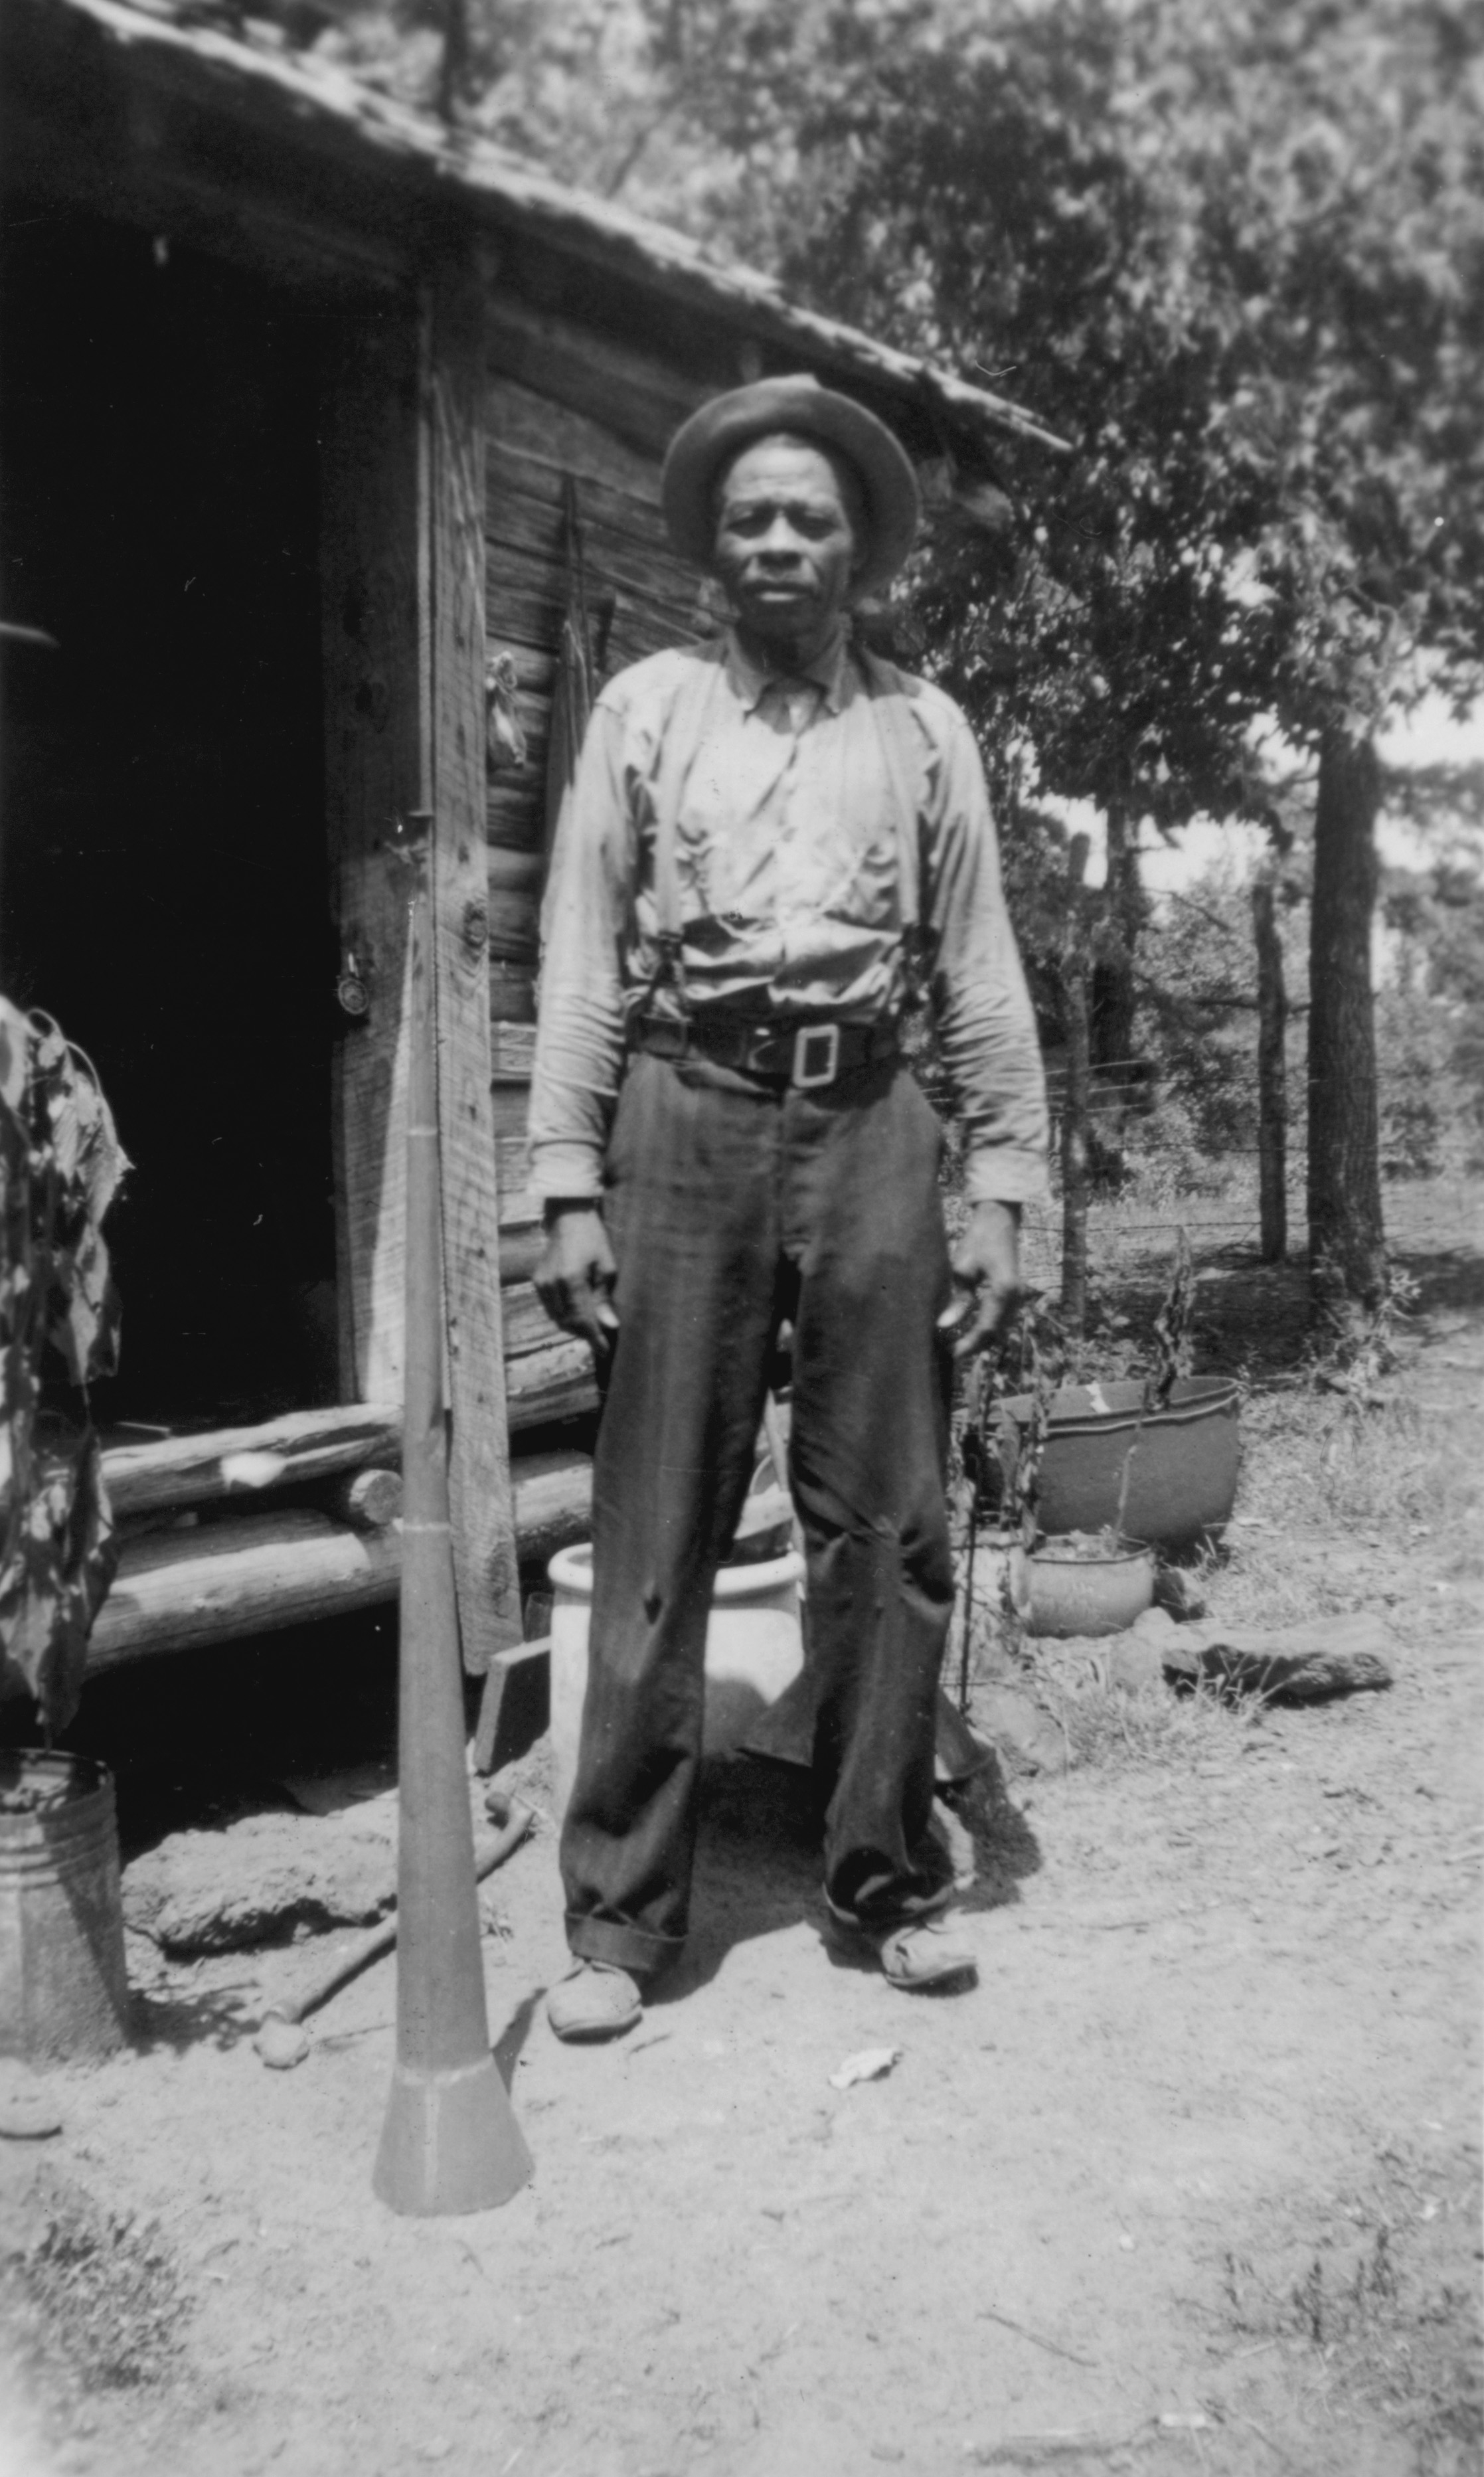
\includegraphics[width=90mm]{./imgs/williswill_recorte.jpg} \label{img9}
\caption{Willis Winn}
%\end{minipage}
\end{figure}

\subsection{Willis Winn, narrativas do Texas, Parte \versal{IV}, página 203}
\label{ref303}

``Vi muitos negros açoitadas nos banquinhos de atar. O que faziam era
dobrar eles à força e amarrar em um banco comprido, amordaçavam a boca
com um pedaço de algodão e então o senhor vinha descer o relho até o
sangue correr pelo chão. Na manhã seguinte, depois do castigo, ele vinha
para a senzala quando você acordava e dizia: `Como é que você está,
menino? Não importa se está doendo, é melhor pular daí e me mostrar que
está firme e forte'. O senhor me odiou até o dia que morreu, pois eu
contei para a senhorinha que ele açoitou uma menina no eito que foi um
escândalo, só porque ela queria voltar para casa e cuidar do bebê
doente. A senhora Callie não nos açoitava, mas ela torcia nossas orelhas
e o nariz até quase arrancar. Aqueles dedos pareciam umas pinças\ldots{}

Eles estavam sempre vendendo escravos, colocando a leilão e vendendo,
dependendo de quanto trabalho conseguiam fazer em um dia e a força que
tinham. Vi muitos deles acorrentados, como se fossem vacas e mulas. Se
um dono tinha mais do que precisava, ele pegava a estrada com eles e
vendia para as fazendas vizinhas. Nenhum nunca fugiu. Não tinham para
onde. Vi muitos e muitos tentarem. Se os patrulheiros não pegavam, algum
branco prendia você e chamava o senhor. Eles tinham um acordo de ficar
de olhos abertos para os negros fujões. Quando o senhor o levava de
volta para casa e terminava o serviço, agora você ficava em casa''.

\subsection{Ben Simpson, narrativas do Texas, Parte \versal{IV}, páginas 27--29}
\label{ref240}

``Chefe, eu nasci na Geórgia, em Norcross, e estou com noventa anos. O
nome do meu pai era Rogert Stielszen e o da minha mãe era Betty. O
senhor Earl Stielszen os capturou na África e levou para a Geórgia. Ele
foi morto, então minha mãe e eu fomos para o seu filho. O filho dele era
um assassino. Ele se encrencou lá na Geórgia, então arranjou dois
cavalos bem rápidos e uma carroça coberta, então acorrentou todos os
seus escravos e fez eles caminharem até o Texas. Minha mãe e minha irmã
tiveram que caminhar. Emma era a minha irmã. No meio da estrada começou
a nevar, mas o senhor não deixou a gente amarrar nada ao redor dos
nossos pés. A gente tinha que dormir no chão também, com toda aquela
neve.

O senhor tinha um chicote de couro cru trançado, bem grande e comprido,
e quando um dos negros ficava para trás ou caía, ele atacava com aquele
chicote. Tirava carne todas as vezes que ele acertava um negro. Minha
mãe não aguentou mais no caminho, mais ou menos na fronteira do Texas.
Os pés dela ficaram sangrando em carne viva, as pernas se incharam até
perder a forma. O senhor só puxou a arma e atirou nela, e enquanto
estava morrendo no chão ele chutou ela duas, três vezes, dizendo:
`Maldita negra, não aguenta nada'. Chefe, pois sabe que aquele homem não
enterrou mamãe, só deixou ela atirada lá onde matou ela. Naquela época
não tinha lei nenhuma contra matar negros escravos''.

\subsection{Essex Henry, narrativas da Carolina do Norte, Parte~I,~páginas~396--97}
\label{ref136}

``O Sr. Henry, irmão do Sr. Jake, e o seu Tio Moses, costumavam passar
um dia inteiro na casa de visita. O Sr. Henry era baixinho, com uma
perna curta e outra comprida, e ele tinha o pior humor que já se viu
nesse mundo. E ele adorava ver os escravos sofrerem, quase tanto quanto
adorava o conhaque. Quando enxergava ele vindo, a gente sabia que ia ter
uma festa da chibata antes dele ir embora.

Tinha três negros, John Lane, Ananias Ruffin e Dick Bogers, que levavam
a culpa por tudo que acontecia naquele lugar. Por exemplo, o Sr. Henry
olhava para o chiqueiro e dizia que parecia que os porcos do seu irmão
estavam minguando o tempo todo. Então o Sr. Jake dizia que eles haviam
sido roubados.

`Por que você não castiga aqueles crioulos ladrões, Jake?'

Jake ficou brabo e mandou trazer esses três negros, arrancar as camisas
deles e prender eles de barriga para baixo. Quando o feitor ficou
cansado, eles deixaram os negros lá, amarrados no sol, e foram para a
casa tomar um conhaque.

Quanto mais eles tomaram da jarra branca, mais ficaram de bom humor.
Eles riram e conversaram e depois de um tempo lembraram dos negros,
então voltaram e bateram neles mais um pouco. Isso durou o dia inteiro,
porque eles se divertiam com a surra''.

\subsection{Spencer Barnett, narrativas do Arkansas, Parte~I,~página~117,~155} \label{ref18}

``Quando era menino, eu escutava os homens perseguindo os escravos com
cachorros pelas montanhas. Os fazendeiros pagavam os patrulheiros para
cuidar dos escravos, manter eles em casa noite e dia.

Era ruim a escravidão. O senhor Tom Williams não era cruel. Ele
nunca tirava sangue. Quando o berrante soava, era melhor estar todo
mundo no lugar. Eles usavam um chicote de couro trançado. Quando ele era
amarrado e molhado, doía de matar. Uma coisa importante era que você
precisava estar no seu lugar, dia e noite. Era um confinamento''.

\subsection{John Eubanks, narrativas do Indiana, página 74} \label{ref84}

```Eu lembro', ele continuou, `como amarravam o escravo ao redor de um
poste, com as mãos amarradas juntas ao redor, e então um grandalhão
pegava um chicote de couro de cobra e açoitava ele até as costas estarem
cortadas e sangrando, o sangue salpicado, gesticulando com aquelas mãos
estranhas de grande, as costas recortadas. Depois eles derramavam
salmoura em cima, que secava e endurecia e grudava nas feridas. Eles não
lavavam até curar. Às vezes, eu via o senhor Everett pendurar um escravo
na pontinha dos dedos. Ele o amarrava de um jeito que ele tinha que
ficar na ponta dos dedos e deixava ele assim'".

\subsection{John White, narrativas do Oklahoma, páginas 323--24}
\label{ref283}

``Meu trabalho era cozinhar. Lavar também. (\ldots{}) Aprendi a tomar
cuidado com os riscos nas roupas. Aprendi com a chibata. Um dia, meu
senhor achou um risco de sabão na sua camisa, então ele me pegou.

A Estrada Militar corre ao lado da fazenda. O senhor me levou estrada
abaixo e me amarrou a uma árvore. Primeiro ele arrancou a camisa velha e
então me açoitou. Quando cansou de me bater, lá veio mais tortura. A
cura da salmoura. Não cura nada, mas é assim que os brancos chamavam.
`Toma', o senhor disse, e atirou a salmoura nas feridas abertas. `Toma!'
As bolhas estouravam cada vez que ele me atirava a salmoura.

Então ele me soltou para ir de volta para a cozinha, cambaleando. A
senhora não podia fazer nada, só passar uma boa graxa, com umas
gentilezas para ajudar com a tristeza''.

\subsection{Rev. Wamble, narrativas do Indiana, página 200}
\label{ref277}

``A mãe do Rev. Wamble era escrava em Deerbrook, e quando o reverendo
tinha dois anos de idade, a mãe morreu de um aborto causado pela
chibata. Quando as escravas estavam em estágio avançado de gravidez,
eles faziam elas deitar de barriga para baixo em uma buraco escavado no
chão especialmente para isso e então eram açoitadas. Fora isso, elas
eram tratadas iguais aos homens. Os braços eram amarrados ao redor de um
cedro ou um poste e elas eram açoitadas''.

\subsection{Mingo White, narrativas do Alabama, página 416}
\label{ref285}

``Lembro que uma vez o velho Ned White foi pego rezando. Os capatazes
pegaram ele no dia seguinte e arrastaram para as estacas, lá onde já
estavam cravadas no chão. Fizeram o Ned tirar tudo, menos as calças, e
deitar de barriga para baixo entre as estacas enquanto amarravam os
braços e as pernas dele às estacas. Depois chicotearam ele até o sangue
correr como se ele fosse um porco. Fizeram todos os escravos irem ver
ele e disseram que a gente ia levar o mesmo castigo se nos pegassem. Não
se deixa ninguém tratar um cavalo como se tratava a gente naquele
tempo''.

\subsection{Susan Hamilton, narrativas da Carolina do Sul, Parte~\versal{II},~página~235}
\label{ref119}

``Quando qualquer escravo era açoitado, todos os outros escravos eram
forçados a assistir. Vi mulheres serem penduradas do teto do edifício e
açoitadas só com alguma coisa ao redor da metade de baixo do corpo até
baixarem ela sem um sopro de vida no corpo. Eu tive umas experiências
horríveis''.

\subsection{George Womble, narrativas da Geórgia, Parte~\versal{IV},~páginas~190--91}
\label{ref308}

``Tinha sempre uma boa quantidade de chibatadas nessa fazenda {[}no
Condado de Jones, centro da Geórgia{]}. Era praticamente a única forma
de castigo usada. Quase todos eram açoitados por serem desobedientes ou
por serem agitados. O Sr. Womble ouviu seu senhor dizer que não teria um
escravo que não conseguisse governar e para garantir que todos os
escravos se admirassem dele e da sua família, a ponto de fazer todos
irem prestar seus respeitos às crianças brancas recém"-nascidas um dia
depois do nascimento. Quando isso acontecia, eles eram obrigados a fazer
fila no lado de fora da porta e então, um a um, entrar no quarto e
baixar a cabeça quando passasse pela cama e dizer `senhorzinho' ou, se o
bebê fosse menina, `senhorinha'. Uma vez, o Sr. Womble diz que ele viu
seu senhor e um grupo de outros homens brancos surrarem um escravo
desobediente até suas costas estarem em carne viva e então aplicarem uma
barra de ferro em brasa. Mesmo isso não tornou o escravo submisso, pois
ele fugiu imediatamente. Após esse tratamento desumano, diversos
escravos fugiram, especialmente na fazenda dos Ridley. Alguns foram
pegos, outros não. Um dos escravos na fazenda dos Womble pegou sua
esposa e fugiu. Ele e a esposa moraram em uma caverna que encontraram no
mato e criaram sua família lá. Quando a liberdade foi declarada e essas
crianças viram a luz do dia pela primeira vez, elas quase ficaram cegas,
o Sr. Womble afirmou''.

\subsection{Clayborn Gantling, narrativas da Flórida, páginas 141--42} \label{ref99}

``Eles tinham os chamados `patrulheiros', que pegavam você longe de casa
e `gastavam' você antes de mandar de volta para o senhor. Se um senhor
tinha escravos que não conseguia controlar (alguns eram fortes e
simplesmente não escutavam o capataz), ele perguntava se o homem queria
visitar outra fazenda. Se ele dizia sim, o senhor dava um passe, e no
passe estava escrito: `Dê uma lição nesse crioulo'. É claro que quando
os patrulheiros ou outro capataz de fazenda lia esse papel, o negro era
espancado quase até a morte e então mandado de volta. O negro não sabia
ler, é claro, e não sabia o que dizia no passe. Eles não deixavam negro
nenhum ter livro ou pedaço de papel, seja qual fosse, e não ensinavam
ninguém a ler''.

\subsection{Charlie Aarons, narrativas do Alabama, páginas 2--3} \label{ref01}

``Tio Charlie disse que o Sr. Harris era um senhor bem áspero, e um
tanto avarento. Todas as rações eram pesadas e limitadas. Ele tinha um
feitor branco e um capataz negro, que era o mais malvado de todos.

Tio Charlie disse que levou muitos sacos de algodão em grandes trens de
mulas de Newton Station até Enterprise, Mississippi. Quando questionado
sobre se isso não oferecia a possibilidade de fugir, ele respondeu:

`Fugir? Ora, minha senhora, aqueles cachorros pegavam a gente, e tudo
que se ganhava era uma surra'.

Tio Charlie pareceu olhar ao longe e então disse: `Sabe, senhora, nunca
vi um escravo ser repreendido até vir para o Mississippi', e eu não
compreendi imediatamente. Então ele riu e disse: `Meu Deus, senhora,
alguns daqueles negros eram bem cabeçudos, e o capataz negro passava
trabalho para tocar eles'".

\paragraph{Comentário}\quad
{\small
O preconceito racial virulento que existia nos Estados Unidos
sustentava e reforçava a escravidão e ao mesmo tempo desculpava e
possibilitava boa parte da crueldade que existia nesse regime. Em
comparação com muitas áreas escravistas no Brasil e no Caribe, a
proporção de brancos em relação a negros era muito maior nos Estados
Unidos. A população americana de negros livres também era pequena, e o
racismo unia os brancos na tentativa de oprimir e controlar os negros.
Assim, os escravizados viviam sob vigilância constante, e os brancos tinham
um grau considerável de liberdade para bater ou maltratar qualquer
pessoa negra. A violência garantia a supremacia da raça branca. Dessa
forma, as motivações raciais emergiam em muitos atos de crueldade, e os
escravizados notavam explícita e implicitamente esse elemento nos seus
maus"-tratos. Diversas narrativas também são comentários diretos ou
indiretos sobre a natureza racista da violência.
}

\subsection{Henry Wright, narrativas da Geórgia, Parte \versal{IV}, página 201}
\label{ref318}

``Na fazenda dos House havia um escravo mulato que deveria receber a sua
liberdade quando fizesse 21 anos de idade. Quando esse dia chegou, o Sr.
House se recusou a alforriá"-lo, então ocorreu uma tentativa de incendiar
a mansão dos House. O Sr. Wright lembra de ver o xerife chegar da cidade
e levar esse escravo. Mais tarde, ouviu"-se falar na fazenda que o
escravo fora enforcado''.

\subsection{William McWhorter, narrativas da Geórgia, Parte~\versal{III},~páginas~96--97}
\label{ref189}

``Minha Tia Mary pertencia ao senhor John Craddock. Quando a mulher dele
morreu e deixou um bebezinho, que era a senhorinha Lucy, Tia Mary estava
dando de mamar para o seu próprio bebê, então o senhor John fez ela
deixar o bebê dele mamar também. Se Tia Mary estava alimentando o
próprio bebê e a senhorinha Lucy começava a chorar, o senhor John
arrancava o bebê dela pelas pernas e dava uns tapas, então mandava Tia
Mary amamentar o bebê dele primeiro. Tia Mary não podia responder com
uma palavra que fosse, mas mamãe diz que muito viu Tia Mary chorar até
as lágrimas se juntarem embaixo do queixo.

Nunca ouvi falar de cadeia nos tempos da escravidão. O que se fazia
naquela época era espancar os negros quase até a morte para fazer eles
se comportarem. Mamãe foi trazida para Bairdstown e vendida em leilão
para o senhor Joe muito antes de eu nascer, mas eu nunca vi escravo
nenhum ser vendido. Meu Deus, minha senhora, nunca ninguém lhe contou
que era contra a lei ensinar um negro a ler e a escrever nos tempos da
escravidão? Os brancos lhe cortavam a mão fora por essas mais do que por
quase qualquer outra coisa. Isso é só jeito de dizer, cortar a mão fora.
Ora, senhora, um negro sem mão não ia ter como trabalhar muito, e o dono
não ia conseguir vendê"-lo por um preço nem parecido com o que ganharia
por um escravo com mãos boas. Eles só espancavam ele a valer quando o
pegava estudando como se faz para ler e escrever, mas eu ouvi falar de
alguns donos que cortavam um dedo cada vez que pegavam um escravo
tentando aprender. Por outro lado, alguns negros queriam tanto aprender
que fugiam de noite e se encontravam em uma ravina profunda onde
estudavam à luz de tochas de acácia. Mas uma coisa era certa, era melhor
eles não deixarem os brancos descobrirem. E se tinham sorte de continuar
com isso até aprenderem a ler a Bíblia, eles guardavam bem o segredo''.

\subsection{Tom Hawkins, narrativas da Geórgia, Parte \versal{II}, página 131}
\label{ref126}

``Não havia escolas onde os escravos podiam estudar naquela época. Eles
eram até proibidos de aprender a ler e escrever. Quando o Dr. Cannon
descobriu que o seu cocheiro aprendera a ler e escrever enquanto levava
e trazia os filhos do doutor da escola, ele mandou cortar os dedões do
negro e colocou outro menino para ser cocheiro no lugar dele''.

\subsection{Ex"-escravizados sobre maus"-tratos, compilado por Louise Oliphant, narrativas
da Geórgia, páginas 292--93}

``Outro ex"-escravo lembrou que `você tinha que chamar os filhos do
senhor de senhor ou senhora, mesmo os bebês. Você nunca vestia roupa o
suficiente e sempre sofria com o desconforto. A gente não tinha
permissão nem para acender o fogo. Se você tinha uma lareira em casa,
ela era tirada e o buraco era fechado. Quem era pego com fogo era
espancado quase até morrer. Muitas mães morreram em cativeiro porque se
resfriaram por não poderem fazer fogo'".

\subsection{Mingo White, narrativas do Alabama, páginas 417}
\label{ref286}

``Os brancos não nos ensinavam nada, só a trabalhar. Eles diziam que
aprender a ler e a escrever não era para nós. Tinha um rapaz chamado E.
C. White que aprendeu a ler e escrever durante a escravidão. Ele tinha
que carregar os livros das crianças para a escola e voltar para
buscá"-las depois. O seu senhorzinho ensinou ele a ler escondido do pai e
do resto dos escravos. A gente não tinha para onde ir, só a igreja, e
isso não nos dava nenhum prazer, pois a gente era proibido de falar do
instante que saía de casa até voltar. Quando a gente ia para a igreja,
os feitores iam junto. Não tinha uma igreja nossa, só a igreja dos
brancos''.

\subsection{Rev. Wade Owens, narrativas do Alabama, página 306}
\label{ref207}

``O senhor Berry e a senhora Fanny Owens eram bons para os negros. Papai
era o cocheiro da senhora Fanny, mas tinha que tomar cuidado com aquele
tal de Ben Boddy, o feitor. Era o homem mais malvado a quem Deus já deu
vida. Ele não nos deixava acender a lareira, por mais frio que fizesse,
e a gente tinha que trabalhar igual ou os cachorros não falhavam. Se o
cachorro não pegava, então eles espancavam quase até a morte. Ele era
tão malvado que o senhor correu com ele da fazenda''.

\subsection{Lucy Brown, narrativas da Carolina do Norte, Parte~\versal{II},~páginas~153--54} \label{ref37}

``Mamãe dizia que a escravidão era muito pior antes dos tempos que eu
lembro. Ela me contou que algumas das escravas tinham os filhos no eito,
que nem as vacas fazem. Ela disse que antes dos bebês nascerem, elas
amarravam a mãe de barriga para baixo quando tinham que açoitar ela,
para não arruinar o bebê''.

\subsection{Lizzie Johnson, narrativas do Indiana, página 115}
\label{ref163}

``O que esses primeiros colonos mais queriam era que seus filhos
aprendessem a ler e a escrever. Muitos deles foram pegos tentando
aprender a escrever, e tiveram seus polegares esmagados, de modo que não
pudessem segurar um lápis''.

\subsection{Cornelia Andrews, narrativas da Carolina do Norte,\break Parte I, páginas 28--31} \label{ref07}

```Se eu fui muito castigada? Não, senhora, eu não fui'. (Aqui a
filha, formada pela Universidade de Cornell, que estava na sala
escutando, se aproximou. `Abre a camisa, mamãe, e deixa a senhora
decidir ela mesma'. Os olhos da velha senhora se arregalaram e ela se
empertigou. Ela parecia envergonhada, mas a filha tirou sua camisa,
expondo as marcas nas costas e nos ombros, que pareciam ter sido feitas
por um chicote de couro trançado. Não havia dúvida alguma disso.)

`Eu fui açoitada em público', ela disse sem alterar a voz, `por quebrar
pratos e por ser lenta. Eu estava com a senhora Carrington naquela
época, logo antes do fim da guerra. Eu estava na cozinha, lavando os
pratos, e deixei um cair. A senhora chamou o Sr. Blount King, um
patrulheiro, e ele me deu o castigo que deixou essas marcas que senhora
vê em mim. Minha velha senhora descobriu e veio me buscar'.

Uma amiga da entrevistada que estava presente observou: `Isso deve ter
sido horrível, para dizer o mínimo'.

`Você não sabe de nada', a velha negra disse, enfurecida. `Alex Heath
foi espancado até a morte aqui em Smithfield. Ele tinha roubado alguma
coisa, foi o que me disseram. Bem, ele foi condenado à morte, e a gente
que mandava por lá decidiu matar ele com uma surra. Deram cem chibatadas
nele todas as manhãs nove vezes, e na nona manhã ele morreu.

Daniel Sanders, meu tio, foi espancado até cortarem ele em pedaços. Era
para ele ter sido surrado até a morte, como fizeram com Alex, mas um
dia, depois que espancaram ele e atiraram de volta na cadeia sem camisa,
ele fugiu. Ele correu para o rio no meio do pântano e as varejeiras
limparam as feridas. Ele estava desmaiado quando um branco o encontrou e
levou para casa. Ele morreu dois ou três meses depois disso, mas nunca
conseguiu deixar o corpo direito nem caminhar sem bengala. Só conseguia
se arrastar'".

\paragraph{Comentário}\quad
{\small
Os escravizados se ressentiam da interferência em suas vidas
familiares, mas quase nunca tinham como impedi"-lo. As vendas eram uma
das maiores fontes de tristeza e sofrimento duradouro. Os proprietários
podiam vender mães sem os filhos ou maridos para longe das esposas, sem
consideração a laços familiares ou idade. Foi o que muitos fizeram entre
1800 e 1860.

Havia muitos motivos para as vendas de escravizados. A oportunidade de
obter lucro ou de se livrar de um cativo incômodo motivou muitas
decisões individuais. Às vezes, as famílias escravas eram divididas
porque o dono decidira doar parte das suas ``propriedades'' humanas a um
filho ou filha que estava se casando. As forças econômicas também
alimentaram o comércio negreiro em nível regional. Após a década de
1820, a cultura do algodão cresceu mais nas regiões a oeste da
cordilheira dos Apalaches, nas terras férteis próximas ao Golfo do
México. Lá, os escravistas queriam mais trabalhadores todos os anos, enquanto
nos estados mais antigos e mais ao norte do Sul, como a Virgínia, a
necessidade econômica por escravizados estava em declínio. Isso levou a um
vasto comércio inter"-regional de escravizados. Não existem estatísticas
exatas, mas provavelmente um milhão ou mais de escravizados afro"-americanos
foram vendidos e forçados a se mudar dos estados mais ao Norte para a
região do Golfo nos últimos anos antes da Guerra Civil. Em todos esses
casos, os cativos sofreram com o fato de serem separados de seus
familiares pelo resto de suas vidas.

Ainda mais degradante, dolorosa e humilhante era a interferência
direta nas vidas íntimas sexuais dos escravizados. Muitos escravistas
tiravam vantagem das mulheres que consideravam atraentes. Outros exigiam
que determinados cativos morassem juntos e se acasalassem para produzir
crianças que o proprietário achava que seriam especialmente fortes e
valiosas. Alguns brancos chegavam a usar ``reprodutores'' para
engravidar mais de uma cativa a despeito dos seus desejos e sentimentos.

Como os senhores de escravos, seus filhos ou outros homens brancos
se aproveitavam sexualmente das mulheres escravizadas, nasceu uma quantidade
considerável de crianças pardas. Muitos dos senhores tinham
uma atitude desumana em relação a essas crianças, que consideravam
apenas mais uma fonte de lucros e as tratavam e abusavam como todos os
outros escravizados. Uma minoria dos senhores de escravos reconhecia ter
alguma obrigação com seus próprios filhos, possivelmente tratando"-os
melhor na fazenda ou, em alguns casos, até mesmo os alforriando. Com o
passar dos anos, essa última decisão criou uma diferença entre a
população negra livre (cerca de 250 mil indivíduos em 1860) dos estados
sulistas mais próximos e mais distantes do Norte. Os dos estados mais ao
Norte eram descendentes de cativos libertados logo após a Revolução
Americana e eram, em sua maioria, lavradores ou peões. Nos estados mais
ao Sul, a população negra livre tendia a ser mais urbana e próspera,
muitas vezes com alguma escolaridade ou ofício. Mas muito mais pessoas
negras que tinham pais brancos sofreram todas as consequências da
escravização.
}

\subsection{Charles Crawley, narrativas da Virgínia, páginas 8--9} \label{ref61}

``Bem, quando esses escravos {[}fugitivos{]} eram pegos, vendiam para os
novos senhores levarem para o Sul. Ouvi dizer que os senhores mais para
o Sul eram tão malvados com os escravos que deixavam eles no eito do
algodão até caírem mortos com a enxada na mão e ainda batiam neles de
novo. Ainda bem que tínhamos donos bons.

Tinha uma casa de leilão, vi aqui mesmo em Petersburg, na esquina da
Sycamore com a Bank. Os escravos eram leiloados para quem pagasse mais.
Alguns se recusavam a ser vendidos, quer dizer, leiloados. Meu Deus do
Céu! Vi muito daqueles jovenzinhos brigar e chutar feito loucos. Minha
filha, dava uma pena de ver. Daí algemavam eles e batiam sem piedade. Eu
não gosto de falar daquela época. Me traz uma tristeza lá de dentro. Se
um escravo se rebelava, eles eram açoitados com um chicote de couro
chamado de `bacalhau'. Minha querida, aquele chicote tinha mais ou menos
a largura da sua mão, do polegar ao mindinho, e era cortado em tiras. Já
viu esses chicotes que usam nos cavalos? Bem, também usavam eles.

Você falou alguma coisa sobre como servíamos a Deus. Sim, menina, vou
lhe dizer como fazíamos; nosso costume era rezar em casas diferentes.
Pois veja, você recebia permissão para ir a esses lugares. E tinha que
mostrar a permissão. Se os patrulheiros pegavam você, davam uma surra. É
o que faziam naquela época. Uma patrulha é uma turma de homens brancos
que se juntavam para andar pelo interior caçando escravos, e surrando e
açoitando os que não tinham as suas permissões. O senhor Allen não
deixava ninguém bater nem açoitar os seus escravos, e lidava com
qualquer um que tentasse, então os escravos do senhor se reuniam e
rezavam de casa em casa. Minha filha, assim a gente falava com o meu
Deus tudo o que queria''.

\subsection{Mingo White, narrativas do Alabama, página 413--415}
\label{ref287}

``Me disseram que Chester {[}Carolina do Sul{]} estava cheia de
especuladores comprando escravos para um pessoal do Alabama. Lembro que
me colocaram numa plataforma e passou um monte de gente para apalpar
meus braços e as pernas e o peito e me fizeram um sem"-fim de perguntas.
Antes de levarem os escravos para o posto comercial, o velho senhor
Crawford disse que se alguém perguntasse se a gente já tinha ficado
doente, era para responder que nunca tinha ficado doente na vida. A
gente tinha que mentir muito pelo nosso senhor, senão apanhava.

Os brancos eram duros com a gente. Eles nos surravam por qualquer
coisinha. Não teria sido tão ruim se a gente tivesse conforto, mas viver
como a gente vivia bastava para deixar qualquer um praticamente morto. Os
brancos nos diziam que a gente nasceu para trabalhar para eles e que a
gente estava fazendo isso muito bem''.

\subsection{Campbell Armstrong, narrativas do Arkansas, Parte~I,~página~71} \label{ref11}

``Colocavam você a leilão e vendiam. É bem isso que faziam: vendiam
você. Esses brancos fazem de tudo, fazem tudo que querem. Arrancavam a
sua roupa como se você fosse um bicho qualquer. Você valia mil dólares
antes, agora não vale nem dois centavos. Não se vale nada quando se é
livre''.

\subsection{Cornelia Andrews, narrativas da Carolina do Norte, Parte~I,~páginas~28--29} \label{ref08}

``Sabe, tinha um mercado de escravos enorme em Smithfield naqueles dias,
e também tinha uma cadeia e um pelourinho. Lembro de um homem chamado
Rough qualquer coisa que comprava quarenta ou cinquenta escravos de uma
vez e levava para Richmond para revender. Ele tinha quatro cavalões
pretos presos a uma carroça, e atrás dessa carroça acorrentava os
escravos, e eles tinham que caminhar ou trotar até Richmond. Os
pequeninos o Sr. Rough atirava na carroça e eles iam para o Norte. Dizem
que teve um dia em Smithfield que trezentos escravos foram leiloados.
Dizem que vinha gente de tudo quanto é lugar, até de Nova Orleans, para
aquelas vendas de escravos. Dizem que antes de eu nascer, costumavam
deixar os negros pelados e fazer eles galoparem pela praça para os
compradores poderem ver que eles não tinham cicatrizes e não eram
deformados.

Eu lembro que vendiam as mamães sem os bebês e que não tinha choro
nenhum no ouvido do senhor. Por quê? Ora, pois senão apanhavam até
ficarem roxas, esse é o porquê''.

\subsection{Ex"-escravizados sobre maus"-tratos, compilado por Louise Oliphant, narrativas
da Geórgia, páginas 293--94, 295}

``Meu senhorzinho tentou ficar comigo, e como não fiquei com ele, ele
fingiu que eu tinha feito alguma coisa e me bateu. Eu revidei, porque
ele não tinha o direito de me bater só por não ficar com ele. A mãe dele
ficou braba comigo por revidar e eu contei por que ele me batera, então
ela me mandou para o tribunal para ser açoitada por brigar com ele. Lá
tinha um tronco onde quase todo mundo mandava os seus escravos para
serem açoitados. Esse tronco tinha forma de cruz, e eles amarravam a
roupa ao redor da cintura e deixavam só o corpo nu para o chicote. Não
importava quem via a sua nudez. Então, naquele dia me bateram até eu não
poder sentar. Quando fui para a cama, tive que deitar de barriga para
baixo para dormir. Depois que terminaram de me açoitar, eu disse que não
deviam achar que tinham feito alguma coisa quando tiraram a minha roupa
na frente de toda aquela gente, pois também haviam tirado a roupa das
suas mães e das suas irmãs. Deus fez todos nós, e nos fez todos iguais.

Depois disso não me levaram de volta para casa, me colocaram na Loja do
Traficante de Negros para ser vendida.

{[}No mercado de escravos{]} Todo mundo queria mulheres que
tivessem filhos rápido. Sempre perguntavam se era uma boa reprodutora, e
quando a resposta era sim compravam você acreditando na sua palavra, mas
se já tivesse tido filhos demais, diziam que você não prestava. Se nunca
tivesse tido filho nenhum, o senhor dizia que você era forte, saudável e
boa trabalhadora. Era preciso ter alguma coisa para ser vendida. Às
vezes, se você era bem bonitinha, alguém lhe comprava sem saber nada
sobre você, só por quem você era. Antes do meu velho senhor morrer, ele
tinha uma menina bonita com quem ficava, e não deixava ela trabalhar em
lugar nenhum fora da casa. Nem a esposa dele nem ninguém dizia nada, mas
ninguém era bobo. Ela teve três filhos dele e, quando ele morreu, o
irmão dele veio e levou a menina e as crianças''.

\subsection{Willie Williams, narrativas do Texas, Parte \versal{IV}, página 189}
\label{ref293}

``Naquela fazenda
não se dava permissão para fazer casamento. As pessoas só se casavam,
mas algumas não tinha permissão para casar, porque o senhor queria criar
negros bem grandes, do tipo que consegue trabalhar bastante e que dá
para vender por uma fortuna. Ele tinha umas dez raparigas que não
deixava casar, umas mulheres grandes e fortes, e o doutor examinava a
saúde delas. Depois o senhor escolhia um negro grande e o doutor
examinava ele também. Aquele negro não precisava trabalhar, ele só
ficava de vigia das mulheres, e era o marido de todas elas. O senhor
criava uns belos de uns negros daquele jeito''.

\pagebreak
\thispagestyle{empty}
\movetoevenpage
\thispagestyle{empty}

\begin{absolutelynopagebreak}
\begin{vplace}
\begin{figure}[H]
\begin{adjustwidth}{-1.6cm}{}
  %\centering
  \vspace*{-2cm}
  %\hspace{-0.5cm}
  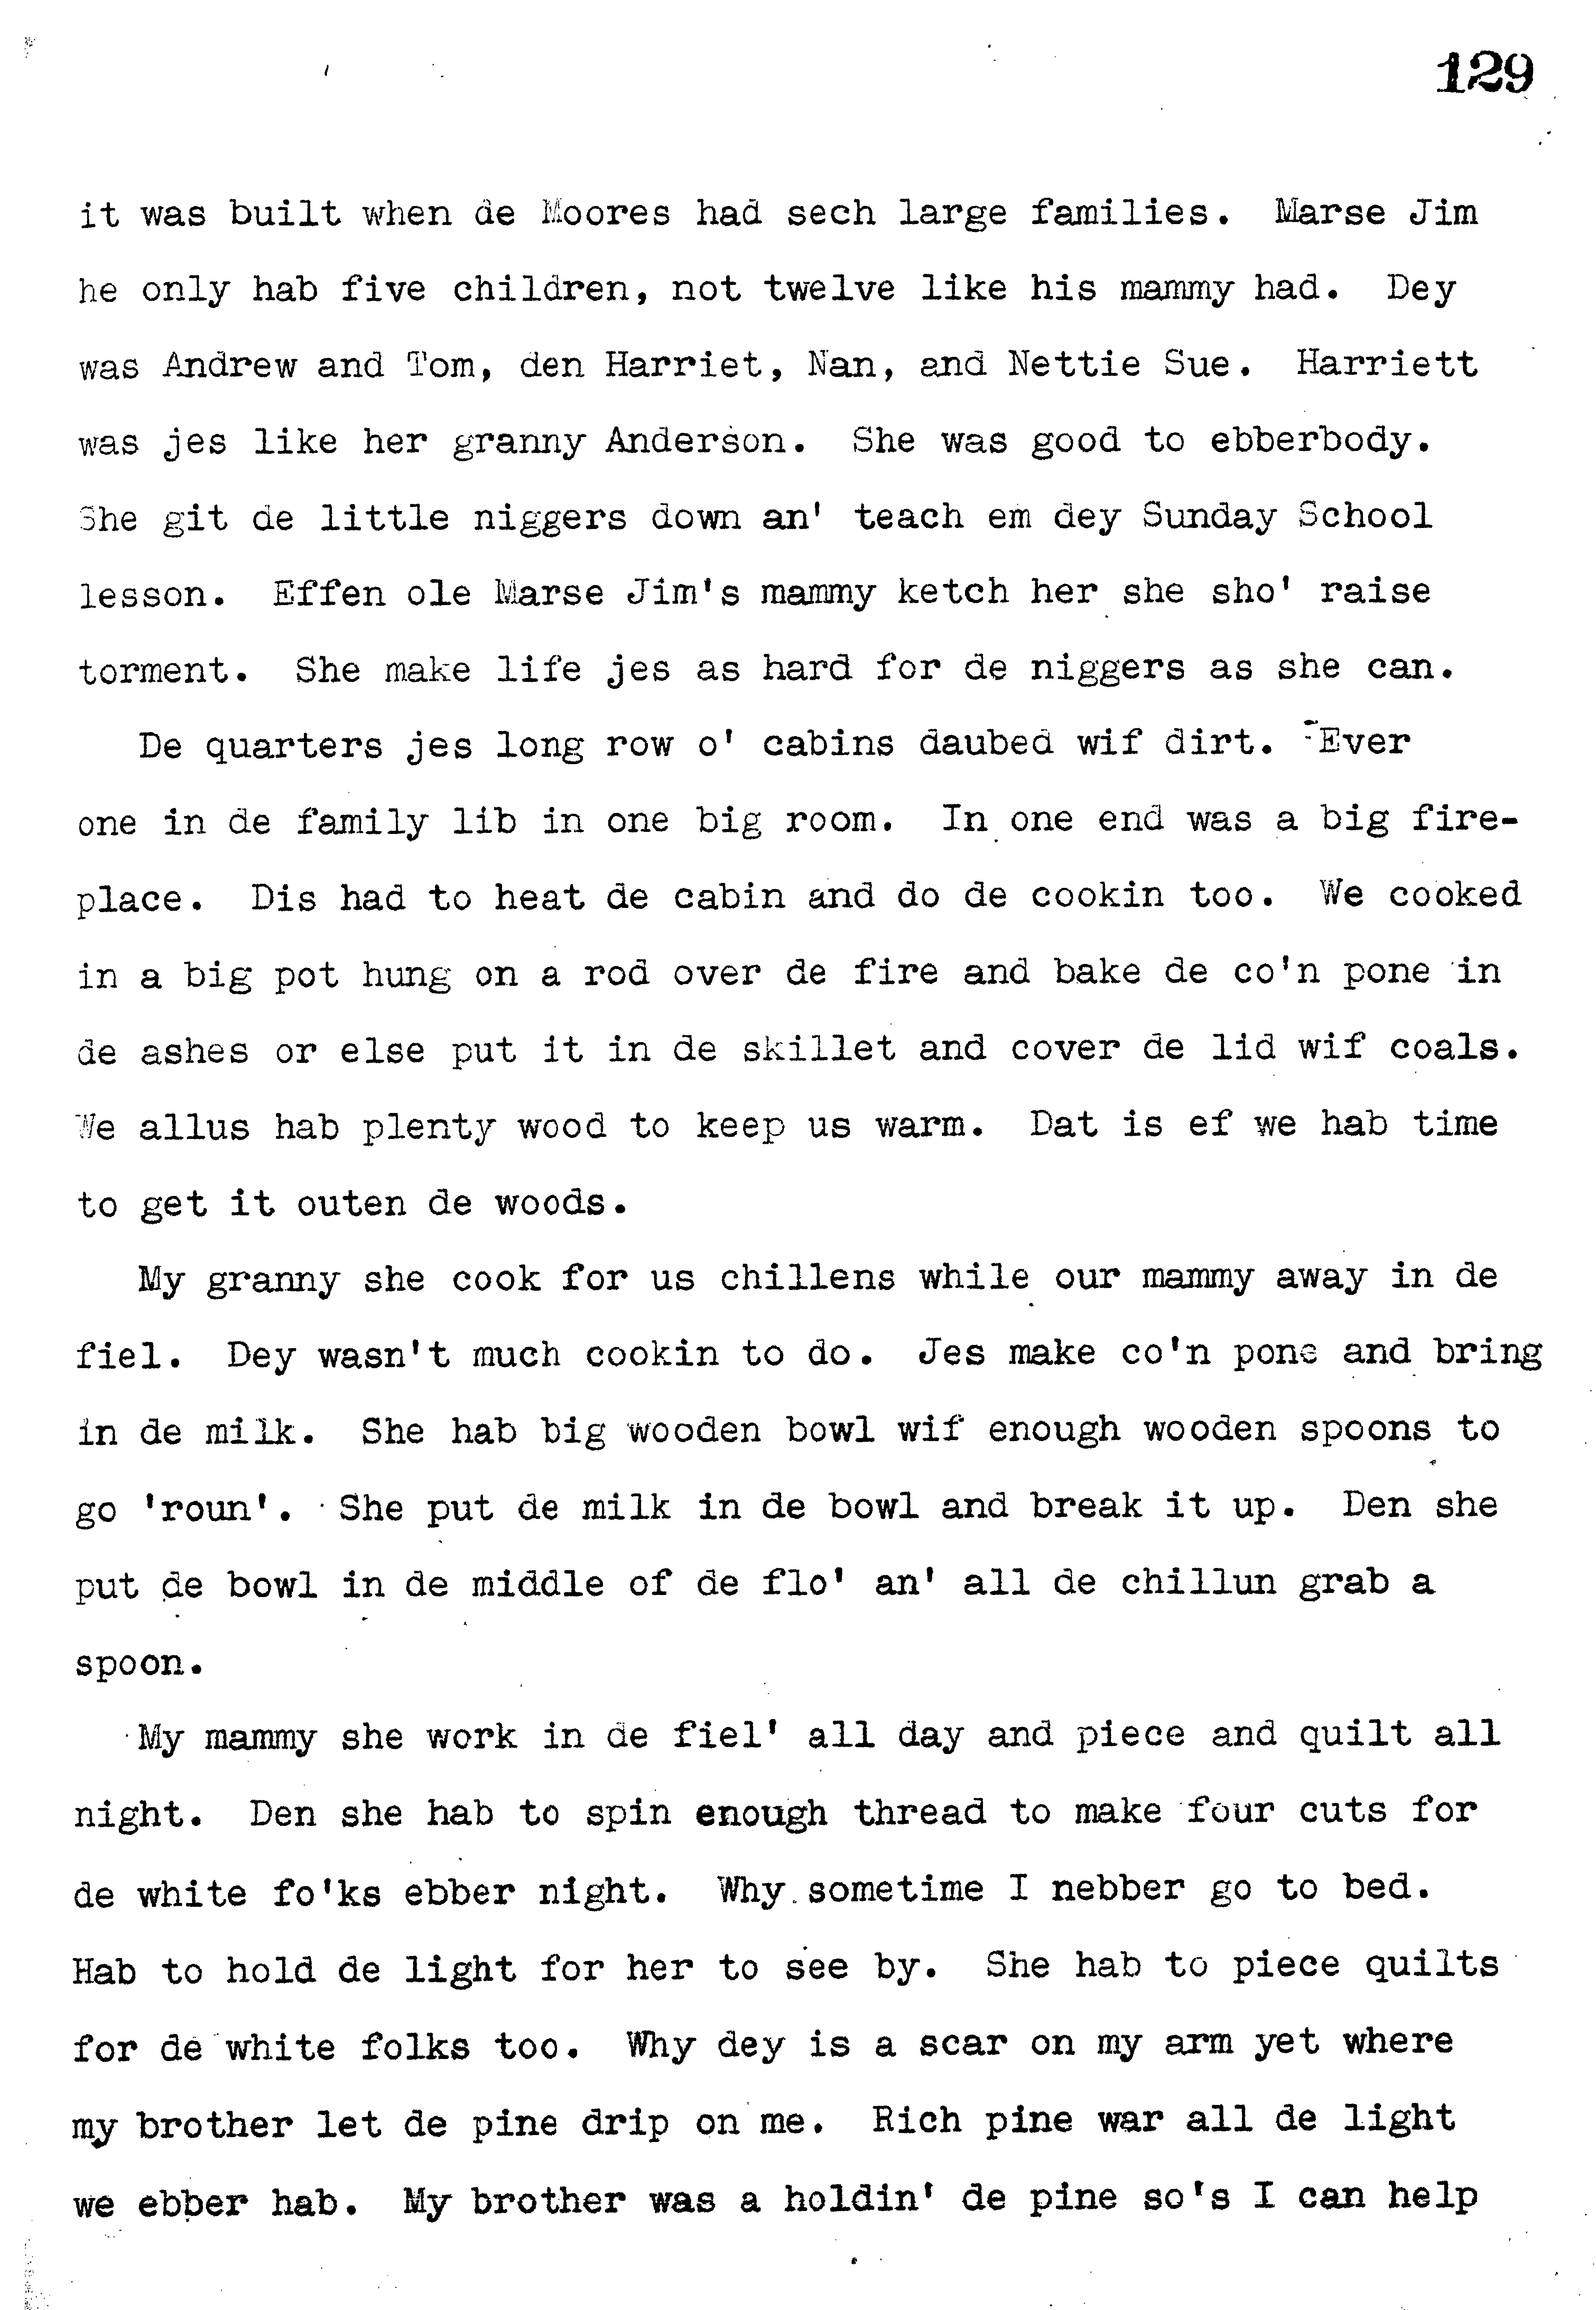
\includegraphics[width=130mm]{./imgs/Cap4.jpg}  
  %\hfill
\end{adjustwidth}
  \caption{Fanny Moore, narrativas da Carolina do Norte, Parte \versal{II}, página 129}
\end{figure}
\end{vplace}

\end{absolutelynopagebreak}

\chapter{Famílias}
%\addcontentsline{toc}{chapter}{{\large\versal{IV.}} Famílias}
%\hedramarkboth{Famílias}{}

\subsection{Fanny Moore, narrativas da Carolina do Norte, Parte~\versal{II},~páginas~129--32}
\label{ref194}

{[}Viveu em situação de escravidão em Spartanburg, Carolina do Sul.{]} ``Mamãe trabalhava no eito o dia inteiro e cerzia e fazia colchas a
noite inteira. Depois ela tinha que fiar o suficiente para quatro cortes
para os brancos todas as noites. Ora, às vezes eu nem ia para a cama.
Tinha que segurar a luz para ela enxergar. Ela tinha que costurar
colchas para os brancos também. Tem uma cicatriz aqui no meu braço, onde
meu irmão deixou a vela de pinho pingar em mim. Alcatrão de pinheiro era
a nossa única luz. Meu irmão estava segurando o pinho para eu ajudar
mamãe a alinhavar a colcha quando ele pegou no sono e deixou ele cair.

Não sei como mamãe aguentou tamanha trabalheira. Mas ela aguentava pelos
filhos. O velho feitor odiava mamãe, porque ela brigava com ele por
bater nos filhos dela. Ora, mas ela apanhou mais por isso do que por
todo o resto. Ela tinha doze filhos. Lembro de ver os três mais velhos
com neve até o joelho, rachando toras enquanto o feitor assistia tudo
rindo. O jeito que eles eram tratados dava uma dor no coração de mamãe.
Todas as noites ela rezava para Deus para tirar os filhos daquele lugar.
Um dia, ela estava arando o algodoal quando deu um grito de repente. Aí
ela começou a cantar e a gritar e a berrar, então parece que começou a
arar ainda mais forte. Quando ela voltou para casa, a mãe do senhor Jim
disse: `O que era tudo aquilo no eito? Você acha que a gente manda vocês
para lá só para ficar gritando? Não, senhora, vocês estão lá para
trabalhar, e é melhor trabalhar, se não o feitor vai descer o chicote
nessas costas'. Mamãe só abriu um sorrisão na cara negra e enrugada
dela. `Eu fui salva, o Senhor me disse que me salvou. Agora sei que Ele
vai me mostrar o caminho, que não vou mais chorar. Por mais que vocês
batam em mim e nos meus filhos, o Senhor vai me mostrar o caminho. E um
dia nós não vamos mais ser escravos'. Vovó Moore puxou o chicote e
lascou nas costas de mamãe, mas mamãe não gritou nenhuma vez. Ela só
voltou para o eito, cantando.

Mamãe chorou muito por George, meu irmão que morreu de febre. Vovó
cuidou dele o melhor que pôde, sempre que escapava da cozinha dos
brancos. Mamãe nunca conseguia ir vê"-lo, só quando chegava em casa de
noite. George só ficava deitado. Um dia, ele estava com um olhar tão
descansado, eu achei que tinha pegado no sono, então deixei ele em paz.
Bem mais tarde, tentei acordá"-lo. Encostei no rosto dele, mas ele estava
morto. Mamãe só foi saber quando chegou de noite. Pobre mamãe, se
ajoelhou no lado da cama e chorou até não poder mais. Tio Allen fez um
caixão de pinho e levou George até o cemitério na colina. Mamãe só ficou
arando e chorando enquanto via eles enterrarem meu irmão.

Papai era ferreiro. Ele ferrava todos os cavalos da fazenda, trabalhava
tanto que não tinha tempo para ir para o eito. O nome dele era Stephen
Moore. O senhor Jim chamava ele de Stephen Andrew. Ele foi vendido para
os Moore, e a mãe dele também. Ela foi trazida da África, nunca aprendeu
a falar normal. Toda a vida ela foi escrava. Os brancos nunca
reconheceram nenhum deles, era o mesmo que se fossem cachorros.

Era um sofrimento ver os especuladores chegando na fazenda. Eles andavam
pelos campos e compravam todos os escravos que queriam. O senhor Jim
nunca vendeu papai nem mamãe nem nenhum dos filhos deles. Ele sempre
gostou de papai. Quando o especulador chegava, todos os escravos
começavam a tremer. Ninguém sabia quem ia embora. Às vezes, eles pegavam
uns para vender no leilão. A parideira sempre rendia mais dinheiro que o
resto, até que os homens. Quando botavam ela a leilão, sempre colocavam
todos os filhos ao redor para mostrar como ela conseguia ter filho
rápido. Depois que era vendida, a família nunca mais via ela. Ela nunca
sabia quantos filhos tinha. Às vezes ela tinha filhos negros, às vezes
brancos. Não adiantava dizer nada, ela só levava o chicote se falasse.
Ora, na fazenda dos Moore, a Tia Cheney, todo mundo chamava ela de Tia
Cheney, tinha dois filhos do feitor. O nome do feitor era Hill. Ele era
mau feito o diabo. Quando Tia Cheney não fazia o que ele mandava, ele
contava para Vovó Moore. A velha chamava Tia Cheney para a cozinha,
fazia ela tirar as roupas e então batia até deixar ela toda roxa. Muitos
meninos e meninas casaram com os próprios irmãos e irmãs sem nunca
saber, a menos que conversassem sobre os pais um do outro e onde moravam
antes''.

\paragraph{Comentário}\quad
{\small
Para os escravizados que viviam sob as condições brutais da
escravidão, os laços familiares eram de suma importância. Eles
representavam uma fonte de força e apoio em meio à injustiça e aos
maus"-tratos do cotidiano. O fato de os casamentos escravos não terem
legitimidade legal ou religiosa não diminuía em nada a sua importância.
Nos laços entre marido e mulher ou entre pais e filhos, os escravizados
encontravam afeto, lealdade, dedicação, alegria e os meios de resistir à
desesperança e acreditar na possibilidade de mudanças no futuro.
Entretanto, a escravidão solapava a vida da família escrava e rompia
muitos dos laços que são tão importantes para qualquer ser humano.

Mais de 21\% dos entrevistados informaram que sua
família fora desfeita durante os anos de escravidão. Em vista ao fato de
que muitos dos informantes eram jovens quando a escravidão foi abolida,
essa porcentagem certamente é baixa demais para ser uma representação
fiel da experiência dos escravizados como um todo. Quando o governo federal
os ajudou a registrar seus casamentos ao final da Guerra Civil,
mais de 40\% descreveram algum tipo de perturbação das suas famílias. 

Como mencionado no capítulo ``Crueldade e castigos físicos'', esses eram os custos humanos do gigantesco comércio negreiro inter"-regional, que todos os anos
enviava milhares de negros dos estados mais antigos na costa do
Atlântico para a região fértil em torno do Golfo do México. Em estados
como a Virgínia e as Carolinas, a população escrava crescia mais
rapidamente do que a demanda econômica por mão de obra. Esse
fato deu aos proprietários na costa do Atlântico a oportunidade de obter
lucros consideráveis com a venda de escravizados para estados algodoeiros
como o Alabama e o Mississippi, onde os proprietários de terras queriam
mais mão de obra cativa. Em linhas gerais, os estados mais antigos eram
``criadouros'' de escravizados para as regiões mais novas, sendo que alguns
escravistas interferiam mais diretamente na vida íntima dos escravizados na
esperança de produzir trabalhadores mais fortes. A ganância rompeu os
laços familiares dos afro"-americanos a serviço do lucro, representado,
nas narrativas, pela figura do ``especulador'', eufemismo para
traficante negreiro.

Os entrevistados para as narrativas do \versal{FWP} culpavam a
venda de familiares por mais de metade de todos os eventos que
desmancharam suas famílias. Outros motivos incluíam a decisão de um
proprietário de dar parte dos seus cativos para um dos seus próprios
familiares, a divisão da herança após a morte do proprietário, a decisão
de um proprietário de se mudar quando parte da família pertencia a outro
indivíduo e diversas outras causas.

Uma simples lista das causas da desestruturação familiar não tem
como sugerir o custo emocional envolvido, a dor e o sofrimento causados
por tais eventos. As narrativas do \versal{FWP} demonstram que os laços
familiares eram extremamente importantes, mas também vulneráveis e sob
ameaça constante, para a maioria dos escravizados.
}

\subsection{Cordelia Thomas, narrativas da Geórgia, Parte~\versal{IV},~página~22}

{[}Viveu em situação de escravidão no Condado de Oconee, Geórgia.{]} ``Nunca mais vai ter casamento como tinha nos tempos de antigamente,
porque todos acham que precisam ter mais que demais hoje em dia. Naquela
época, quando se casava, todo mundo estava pensando em fazer uma casa
decente para si, então casar era algo meio que sagrado. Mamãe diz que
quase sempre que os escravos casavam, eles só saltavam para trás por
cima de uma vassoura enquanto o senhor assistia e então ele anunciava
que os dois agora eram marido e mulher''.

\subsection{Sarah Pittman, narrativas do Arkansas, Parte~V,~página~353}

{[}Viveu em situação de escravidão na Paróquia da União, Luisiana. Falando do marido, ela afirma que ele está{]} ``descansando no reino
do Senhor. Ele era diácono da igreja, e a palavra dele valia. A fazenda
inteira escutava ele e fazia o que ele dizia. Todo mundo respeitava ele,
pois ele era direito. Eu só me casei uma vez, e homem nenhum vai ocupar
o seu lugar. Ele foi o primeiro, o melhor e o último''.

\subsection{Barbara Haywood, narrativas da Carolina do Norte, Parte~\versal{II},~páginas~386--88}
\label{ref131}

{[}Viveu em situação de escravidão na Carolina do Sul.{]} ``Quase tudo que eu lhe contar vai ser sobre Frank Haywood, meu marido.

Eu nasci na fazenda de John Walton, onze quilômetros a sudeste de
Raleigh {[}na Carolina do Norte{]}. Handy Sturdivant, meu pai, pertencia
a alguém no Condado de Johnson, mas mamãe e seus filhos pertenciam ao
senhor John Walton.

\textls[-15]{O senhor John fez uma debulhação de milho uma vez, e foi nessa
debulhação que eu vi Frank pela primeira vez. Eu era uma menininha,
chorando e berrando, e Frank, que era um rapaz grande, diz que nunca
quis tanto dar umas palmadas numa pequena, e eu não gostei dele mais do
que ele de mim.}

Ele pertencia ao Sr. Yarborough, que tinha o hotel em Raleigh, mas
trabalhava para qualquer um que contratasse ele, e não sei onde arranjou
o seu nome.

Vi Frank algumas vezes na Igreja Metodista de Holland, onde a gente ia
para a igreja com os nossos brancos. (\ldots{})

Depois da guerra, a gente se mudou para Raleigh, na Rua Davie, e eu
estudei um pouco na Saint Paul. Frank estava trabalhando no Mercado
Municipal na Rua Fayetteville, e eu desviava várias quadras do meu
caminho da escola, de manhã e de noite, para ver ele. Sabe, eu já estava
apaixonada havia um tempão.

Depois de um tempo, Frank virou açougueiro e começou a ganhar bem. Eu
tinha treze anos e ele veio me ver, então um ano depois começou o
namoro. A gente estava sentado na cozinha da casa na Rua Davie quando
ele me pediu para ser dele e eu aceitei.

\textls[-15]{Ele disse que não me merecia, mas que me amava e que faria de tudo para
me agradar, e que sempre seria bom comigo.}

Eu casei quando tinha catorze anos, e quando tinha quinze nasceu
Eleanor, minha filha mais velha. Tive três depois dela, e Frank não
podia ter mais orgulho deles. Fomos felizes. Vivemos juntos 54 anos e
sempre fomos felizes, com uns bate"-bocas de vez em quando. Minha jovem,
espero que você tenha a mesma sorte que eu tive com Frank''.

\subsection{Peter Clifton, narrativas da Carolina do Sul, Parte~I,~páginas~208--09}

{[}Viveu em situação de escravidão no Condado de Kershaw, Carolina do Sul.{]} ``Você pergunta por que quis casar com a Christina. Tinha algo naquela
menina, no dia que conheci ela, apesar de ter meio quilo de algodão
preso no cabelo dela, que me atraiu igual uma mosca que fica rodeando e
pousa na jarra de melaço. Não deixei a poeira assentar na estrada de
Ashford Ferry até conquistar ela. Tive que pedir para os velhos dela
antes dela consentir. Isso levou uns seis meses. Tudo tinha que ser nos
conformes. Finalmente, convenci o pastor, o Reverendo Ray Shelby, a ir
até lá nos casar. Ela foi uma benção em todos os dias da minha vida
desde então''.

\paragraph{Comentário}\quad
{\small
Como indica a história de Peter Clifton, o romance podia ser um
grande desafio, e manter uma família era difícil devido às pressões da
escravidão e ao fato de muitos escravizados casarem com pessoas de fazendas
vizinhas. Um informante no projeto da Fisk University explicou que
``havia dois tipos {[}de casamento{]}. Um era casar em casa e o outro
era casar fora''. 

Havia vários motivos para casamentos entre
pessoas de fazendas diferentes. Alguns indivíduos podiam querer
criar uma distância entre sua vida familiar e a supervisão do seu dono.
Outros simplesmente se apaixonavam por um homem ou mulher que morava nas
redondezas, nas terras de algum outro senhor. Como metade das fazendas
escravistas dos Estados Unidos tinha menos de cinco cativos, muitos
indivíduos simplesmente não tinham outra opção além de procurar um
companheiro ``de fora''.

Os estados escravistas não tinham nenhuma forma de reconhecimento
legal dos casamentos entre cativos, pois isso impediria a livre
dissolução da família escrava por venda, execução de dívida, partilha de
herança ou simples permuta. Por consequência, os casamentos
não recebiam nenhuma proteção e não tinham garantia sequer de que suas
uniões seriam reconhecidas em alguma cerimônia. O senhor de cada
indivíduo decidia se haveria algum reconhecimento público do casal ou se
as cerimônias seriam proibidas. Aparentemente, o tipo mais comum de
``cerimônia'' de casamento para os escravizados era uma prática chamada de
``pular a vassoura'', um ritual popular que, curiosamente, também foi
observado em diversas partes do mundo ocidental. Os cativos certamente
teriam desejado mais, mas muitos não tinham permissão para mais do que
isso.
}

\subsection{Andy Marion, narrativas da Carolina do Sul, Parte~\versal{III},~página~167}
\label{ref182}

``Vou lhe contar, arranjar uma mulher durante a escravidão era um
inferno para os negros. Se não tinha uma que gostasse na fazenda, e é
bem provável que ela não gostava de você, ora, mas o que você poderia
fazer? Não dava para pular da cama, subir na mula e ir até a fazenda
vizinha sem um passe por escrito. Agora imagine que o senhor lhe dá o
consentimento. Pois, o senhor da menina tem que consentir também, a
menina tem que consentir, o pai da menina tem que consentir, a mãe da
menina tem que consentir. Era um trabalhão dos diabos!''.

\subsection{Millie Barber, narrativas da Carolina do Sul, Parte~I,~página~39} \label{ref14}

``Bem, papai pertencia a um homem e mamãe pertencia a outro, a sete ou
oito quilômetros de distância. Isso causava confusão, desentendimentos e
muita angústia. Papai precisava pedir um passa para ir ver mamãe. Às
vezes, ele vinha sem um passe. Os patrulheiros pegaram ele escondido lá
em cima da chaminé uma noite. Arrancaram a roupa dele na frente de mamãe
e deram trinta e nove chibatadas, com ela chorando e berrando mais alto
do que ele''.

\subsection{Caleb Craig, narrativas da Carolina do Sul, Parte~I,~página~231} \label{ref60}

``O homem que tinha uma mulher em outra fazenda não tinha paz nem
felicidade. Ele só via a mulher uma vez por semana, com um passe, e o
ciúme deixava ele distraído o resto da semana, se amava ela bastante''.

\subsection{Callie Williams, narrativas do Alabama, página 426}
\label{ref289}

\textls[-15]{``Papai era capataz, trabalhando sob o feitor, mas mamãe diz que ela
ficava no berçário da senzala e cuidava de todos os bebezinhos. Eles
tinham uma choupana toda arrumada com berços caseiros e coisas assim,
onde colocavam todos os bebês. As mamães vinham do eito às dez horas
para dar de mamar e mais tarde no dia, e minha mãe alimentava os menores
com licor de panela e os mais velhos com verduras e licor de panela.
Eles também tinham leite desnatado e mingau.}

Nosso casamento não foi nada parecido com como mamãe diz que foi o
dela com papai. Ela diz que eles `pularam a vassoura'. Quando um escravo
qualquer queria casar, ele tinha que ir até a casa grande e contar ao
senhor. Ele pegava a sua vassoura e dizia `Harry, você quer a Vicey?' E
Harry dizia `sim'. Então o senhor dizia `Vicey, você quer o Harry?' e
ela dizia `sim'. E então o senhor dizia `Deem as mãos e pulem a vassoura
e vocês estão casados'. A cerimônia não era grande coisa, mas se ficava
muito mais junto naquela época e não se ouvia falar de tantos divórcios
e coisas assim''.

\subsection{Emma Hurley, narrativas da Geórgia, Parte~\versal{II},~página~276}
\label{ref158}

``Não havia casamentos de escravos. Mandava"-se os escravos `pular a
vassoura', muitas famílias foram separadas por vendas. Lembro bem
quando o Sr. Seaborn Callaway veio para a fazenda e comprou minha avó e
alguns outros escravos e levou eles embora. Nós choramos e choramos,
vovó também. Os brancos compravam e vendiam escravos desse jeito o tempo
todo''.

\subsection{George Lewis, narrativas da Geórgia, Parte~\versal{III},~página~49}
\label{ref172}

{[}Viveu em situação de escravidão na Flórida.{]} ``Quando um casal queria casar, o homem obtinha permissão do
proprietário da sua pretendida e, se este consentia, uma vassoura era
colocada no chão. O casal saltava sobre ela e então eram declarados
marido e mulher''.

\subsection{Adeline Willis, narrativas da Geórgia, Parte~\versal{IV},~página~165}
\label{ref298}

{[}Quando Adeline tinha quatorze anos de idade, ela e Lewis se casaram. Ou melhor, o que aconteceu foi o seguinte:{]} ``A gente não teve pastor quando
casou, meu senhor e senhora disseram que não se importavam, e o senhor e
a senhora do Lewis disseram que não se importavam, então todos se
reuniram na casa dos meus brancos, nos chamaram e disseram que não se
importavam se a gente casasse. Meu senhor disse: `Você e o Lewis querem
casar e ninguém tem objeções, então vocês dois podem saltar sobre a
vassoura juntos e estão casados'. Não foi nada além disso, e nós
casamos. Eu continuei morando com os meus brancos e ele com os deles, e
ele continuou a ir me ver, igual fazia quando estava me namorando. Ele
nunca me levou presente nenhum, pois não tinha dinheiro para comprar
nada, mas ele era bom para mim, e era isso que contava''.

\paragraph{Comentário}\quad
{\small
Nas Narrativas de Escravos do \versal{FWP}, a alegria das festas de
casamento é minúscula em comparação com as inúmeras descrições da
aflição das famílias separadas por vendas, por escravizados sendo dados de
presente para outros proprietários e por outros motivos. Fica evidente
que as pessoas sofriam terrivelmente quando suas famílias eram
desfeitas e que se ressentiam dessa prática, considerada uma das maiores
crueldades e injustiças da escravidão nos Estados Unidos.
}

\subsection{Sarah Gudger, narrativas da Carolina do Norte, Parte~I,~páginas~354--55}
\label{ref115}

``Nenhum dos escravos da nossa fazenda nunca foi vendido, mas os da
outra fazenda do senhor William foram. Ah, mas que época horrível era
aquela! Todos os escravos no eito, arando, capinando, cantando e
fervendo no sol. O velho senhor aparecia no campo com um homem que
chamavam de especulador. Eles caminhavam por tudo, só olhando, só
olhando. Todos os negros sabiam o que era aquilo. Eles não tinham
coragem de levantar os olhos, só seguiam trabalhando. Então o
especulador avistava quem ele queria. Ele falava com o velho senhor,
eles prendiam as algemas nele e levavam embora para a terra do algodão.
Ah, mas que época horrível! Quando o especulador estava pronto para ir
embora com os escravos, se tinha algum que não queria ir, ele dava uma
surra, então amarrava atrás da carroça e fazia o negro correr até
desmaiar no chão, depois surrava de novo até ele dizer que ia embora sem
incomodar mais. Às vezes, alguns fugiam de volta para a fazenda, mas daí
era pior para eles do que antes. Quando os negros saíam para almoçar, a
velha negra dizia onde estava esse e aquele. Nenhum dos outros queria
contar a verdade. Mas quando ela via eles baixando os olhos, ela só
dizia: `O especulador, o especulador'. Daí as lágrimas escorriam pela
bochecha, porque podia ser o filho ou o marido e ela sabia que nunca
mais ia ver ele de novo. Ou então talvez eles estivessem deixando
filhinhos em casa, ou só pai e mãe. Ai, meu Deus, meu velho senhor era
mau, mas ele nunca mandou nenhum de nós para a terra do algodão''.

\subsection{Jenny Proctor, narrativas do Texas, Parte~\versal{III},~página~212}
\label{ref218}

{[}Viveu em situação de escravidão no Alabama.{]} ``Às vezes ele vendia alguns dos escravos no leilão para quem desse o
maior lance, quando conseguia ganhar o que chegue.

Quando ia vender um escravo, esse ganhava bastante comida por uns dias.
Quando chegava a hora de levar ele para o leilão, ele pegava um pedaço
de sebo e esfregava bem em volta da boca do negro e fazia parecer que
ele andava comendo bastante carne e coisas assim e era bem forte para
trabalhar. Às vezes, ele vendia os bebês de peito e outras vendia as
mães dos bebês, os maridos das mulheres e assim por diante. Ele não
deixava ninguém chorar muito quando a família era vendida. `Cala a boca
ou vai apanhar', ele dizia. Mas eles amavam muito os seis filhos que
tinham, não iam querer ninguém comprando eles''.

\subsection{Bryant Huff, narrativas da Geórgia, Parte~\versal{II},~página~239}
\label{ref152}

{[}Viveu em situação de escravidão no Condado de Warren, Geórgia.{]} ``Dos 12 filhos em sua família, dois foram vendidos. Harriet, a mais
velha, de propriedade de um juiz que morava em uma fazenda vizinha,
voltou para a família após a Emancipação. O pai saiu de casa em um
acesso de fúria, pois um dos seus filhos fora açoitado. O senhor,
sabendo como ele era dedicado à esposa, colocou ela e o filho pequeno na
cadeia. Logo em seguida, o pai voltou e recebeu permissão para visitar a
esposa e ir embora sem ser incomodado. Algumas semanas depois ele voltou
à cadeia e recebeu permissão para entrar, assim como antes, mas quando
estava prestes a sair, foi informado que deveria ficar lá para sua
segurança. No dia seguinte, ele e Johnie, seu filho, foram vendidos para
especuladores que prometeram levá"-los tão longe que lhes seria
impossível retornar. Quando Daniel estava partindo, ele disse à esposa
para esperar sua volta, demorasse ele meses ou anos. Ela chorou e
lamentou sua partida e se recusou a casar"-se novamente, apesar da
insistência. Alguns meses antes do fim da Guerra Civil, o marido
reapareceu e ficou na fazenda até a emancipação. Johnie morreu em um
acidente logo após a partida''.

\subsection{Thomas Cole, narrativas do Texas, Parte~I,~página~228} \label{ref56}

{[}Ele elogia o seu senhor por não açoitar seus escravos e por ser um
homem muito bom, mas após a morte deste sua senhora{]} ``levou minha mãe
para a cozinha e fui a última vez que vi ela. A senhora Cole comprou uma
casa muito fina em Huntsville {[}Alabama{]}, mamãe me disse para ser bom
e fazer tudo que o feitor mandar. Dei tchau e ela nunca conseguiu voltar
para me ver, e eu nunca mais vi ela nem meu irmão e minha irmã. Nunca
soube se foram vendidos ou não''.

\subsection{Tom Hawkins, narrativas da Geórgia, Parte~\versal{II},~página~130}
\label{ref127}

[Viveu em situação de escravidão na Carolina do Sul.] ``A nossa fazenda tinha entre 150 e 200 hectares. A Dona Annie tinha uns 100 escravos. Ela vivia vendendo eles por um dinheirão depois que
treinava os cozinheiros, criadas, criados, cocheiros e lavadeiras das
boas. (\ldots{}) Sim, moça, eu vi a velha senhora vender os escravos que
treinou. Ela botava eles de pé na plataforma que deixava no pátio dos
fundos quando leiloava eles. Vi vários traficantes passarem pela nossa
fazenda com carroças, onde levavam a comida e a cama, com os escravos
andando atrás da carroça. Eles iam ser vendidos, mas nenhum deles ia
acorrentado''.

\subsection{Addie Vinson, narrativas da Geórgia, Parte~\versal{IV},~página~107}
\label{ref268}

{[}Viveu em situação de escravidão no Condado de Oconee, Carolina do Sul.{]} ``Havia um traficante de escravos chamado McRaleigh que costumava
visitar a fazenda do velho senhor para comprar negros e levá"-los para as
baixadas do Mississippi. A gente fugia para o mato quando via ele vindo.
Ele pegou minha Tia Rachel, dava para ouvir ela berrando na estrada a
mais de um quilômetro de distância''.

\subsection{Elige Davison, narrativas do Texas, Parte~I,~páginas~298--99}

{[}Viveu em situação de escravidão na Virgínia. Ele começa dizendo, em sua terceira frase:{]} ``O senhor e a senhora
eram brancos muito bons e eram muito bons para os negros''. {[}Mas um
pouco depois ele diz:{]} ``Às vezes a gente levava chibatada'' {[}e{]}
``Quando se junta uma boiada para vender os bezerros, como choram as
vacas e os bezerrinhos, era assim que eram os escravos naqueles tempos.
Eles não sabiam nada dos parentes. Criança quase nenhuma sabia quem era
o seu pai, alguns não sabiam da mãe, porque tinham sido tiradas da mãe
quando foram desmamadas, e as crianças eram vendidas ou trocadas para
não tomarem muito gosto pelo pai ou pela mãe.

Vi alguns fugirem para o Norte. Às vezes o senhor pegava eles e colocava
na cadeia. Não dava para ir a lugar nenhum sem um passe. Os patrulheiros
pegavam a gente e faziam e aconteciam com os negros escravos. Eu ia para %e faziam e aconteciam com os negros? Resposta do Francisco, que não entendi: <<"Fazer e acontecer"? "1 Bras. Fazer (alguém) o que quer, o que bem entende." diz o Aulete. Assim como "chegar" para "bastar", pode ser que não seja corrente no paulistês, mas que eu saiba não é gauchismo.>>
a senzala e ficava tão cansado que só caía porta adentro, direto no
chão, e um patrulheiro aparecia com um bacalhau e me chicoteava várias
vezes para ver se eu estava cansado o suficiente para não fugir. Às
vezes os patrulheiros nos batiam só para ouvir a gente gritar.

Quando um escravo morria, ele era só mais um negro morto. O senhor
mandava fazer uma caixa de madeira para colocar o negro e levava ele
para um buraco no chão. A gente marchava três vezes ao redor da
sepultura e era isso''.

\subsection{Lina Hunter, narrativas da Geórgia, Parte~\versal{II},~páginas~20--21}

{[}Viveu em situação de escravidão no Condado de Oglethorpe, Geórgia.{]} ``Sim, senhora, eu vi escravos serem vendidos. Eles só colocavam o negro
a leilão e vendiam para quem desse o lance. Um trabalhador dos bons
rendia um preço alto, e uma boa parideira também trazia bastante
dinheiro, porque os brancos todos gostavam de ter bastante criancinha
com eles. As parideiras essas nunca trabalhavam nada; eles faziam os
outros escravos cuidarem delas até os bebês nascerem. As escravas que
tinham bebês eram mandadas de volta do eito de manhã e depois do almoço
para os bebês poderem mamar até ficarem grandes o suficiente para
comerem pão e leite; depois, eles ficavam com as outras crianças,
cuidadas pela Vovó Rose.

Os escravos nem casavam como se faz hoje. Não tinha essas modernices de
licença para comprar. Tudo que tinham que fazer era dizer ao senhor que
queriam se casar. Se deixava, ele mandava eles pularem por cima de uma
vassoura e os dois estavam casados''.

\subsection{Peter Clifton, narrativas da Carolina do Sul, Parte~I,~página~207}

{[}Viveu em situação de escravidão no Condado de Kershaw, Carolina do Sul.{]} ``O senhor Biggers acreditava no chicote e em fazer seus escravos
trabalharem duro; os homens tinham sempre muito medo de serem vendidos e
separados da mulher e dos filhos. Mas ele mais ladrava que mordia,
porque nunca soube dele fazer uma maldade dessas com ninguém''.

\subsection{John W. Fields, narrativas do Indiana, páginas 77--78} \label{ref90}

{[}Viveu em situação de escravidão em Owensburg, Kentucky.{]} ``Além de mim, tinha mais outros 11 filhos na minha família. Quando eu
tinha seis anos de idade, todos nós fomos tirados dos meus pais, porque
meu senhor morreu e o seu espólio precisou ser liquidado. Nós escravos
fomos divididos pelo seguinte método. Três pessoas desinteressadas foram
escolhidas para ir à fazenda, e juntas elas escreveram os nomes dos
vários herdeiros em alguns pedaços de papel. Esses papeizinhos foram
colocados em um chapéu e passados entre nós escravos. Cada um tirou um
papel e o nome no papel era o novo dono. Por acaso eu tirei o nome de
uma parente do meu senhor que era viúva. Não consigo descrever a
angústia e o horror daquela separação. Eu tinha só seis anos de idade e
foi a última vez que vi minha mãe por mais que uma noite. Doze filhos
tirados de minha mãe no mesmo dia''.

\subsection{Sra. Parthena Robbins, narrativas do~Indiana,~páginas~167--8}

{[}Viveu em situação de escravidão no Condado de Scott, Kentucky.{]} ``Uma vez, quando os `traficantes de negros' vieram, havia uma menina,
mãe de um bebezinho; os traficantes queriam a menina, mas não compravam
ela por causa da criança. O dono afastou a menina do restante da
escravaria, tirou o bebê dela e matou o bebê a pancadas na frente da
mãe, então trouxe a menina de volta já sem o bebê. Ela foi vendida
imediatamente.

Seu novo senhor ficou tão contente em obter uma menina tão forte, capaz
de trabalhar tão bem e tão rápido.

A lembrança do jeito cruel como mataram o bebê assolaram tanto sua mente
que ela desenvolveu epilepsia. Isso irritou seu novo senhor, que
mandou"-a de volta para o antigo e forçou"-o a reembolsar o dinheiro que
ele tinha pago por ela''.

\subsection{Sylvia Cannon, narrativas da Carolina do Sul, Parte~I,~página~188} \label{ref46}

``Vi muita gente negra ser vendida para longe naqueles tempos, porque
era assim que os brancos ganhavam muito do dinheiro dele. É claro que
nunca nos contavam por quanto nos vendiam. Só colocavam os negros em
cima de um bloco de mais ou menos um metro de altura e o especulador
dava o seu lance, como se fossem cavalos. Quem era leiloado nunca dizia
nada. Não sei quem comprou meus irmãos, George e Earl. (Ela chorou após
essa afirmação). Vi venderem escravos duas vezes antes de me venderem e
vi os escravos sendo tocados feito porcos até Darlington. Algumas das
mulheres pareciam que iam cair lá mesmo, de tão grande que estavam {[}em
gravidez adiantada{]}''.

\subsection{Robert Falls, narrativas do Tennessee, páginas 13--14} \label{ref87}

``Minha mãe foi vendida três vezes antes de eu nascer. A última vez,
quando o Velho Goforth vendeu ela para os especuladores de escravos
(sabe como é, cada vez que precisavam de dinheiro, eles vendiam um
escravo), quando estavam levando eles, tocando, igual a uma récua de
mulas, para o mercado, da Carolina do Norte para a Carolina do Sul, ela
começou a ter um ataque. Pois tinham vendido ela sem o bebê, sabe? E bem
assim, ela começou a ter ataques. Eles chegaram na cadeia, onde iam
passar a noite, e ela ficou em tal estado que Jim Slade e Press Worthy,
os dois especuladores, eles não tinham o que fazer com ela. No dia
seguinte, um deles levou ela de volta para o senhor Goforth e disse:
`Escuta aqui, a gente não pode fazer nada com essa mulher. O senhor tem
que pegar ela de volta e devolver o nosso dinheiro. E tem que ser
agora'. E eles estavam falando sério. Então o Velho Goforth ficou com a
minha mãe e deu o dinheiro de volta. Depois disso, nenhum de nós nunca
foi separado. Todos nós, um irmão e duas irmãs e minha mãe, moramos com
os Goforths até a liberdade chegar.

E vou lhe contar, ela nunca mais parou de ter ataques. Ela tinha um
ataque toda vez que a Lua mudava, ou pelo menos de duas em duas Luas.
Mas ela seguiu trabalhando. Era muito trabalhadora, ela. Tinha que ser.
A velha senhora não vacilava. Aquela era mais malvada que o velho
senhor. Ela sentava no lado da roda de fiar e contava as voltas que as
escravas davam. E ela não se deixava enganar. Minha mãe trabalhava até
as dez horas quase todas as noites porque a parte dela era dar tantos
cortes por dia, e não conseguia terminar antes disso''.

\subsection{Joe Higgerson, narrativas do Missouri, páginas 176--77}
\label{ref143}

```Sim, senhora', ele exclamou. `Ora, lá em Boonville {[}no Missouri{]},
uma mulher foi colocada à venda com o bebê e o comprador queria a
mulher, mas não queria o bebê, então separaram os dois. Quando estavam
se preparando para colocar eles no barco para Nova Orleans e descer o
rio, a mulher voltou correndo para dar um beijo de tchau no bebê, então
o traficante puxou um chicote e estalou ele. `A vaca mugidora logo
esquece o bezerro!', ele gritou. Ela foi vendida rio abaixo e nunca
mais viu o bebê. Isso foi triste'. Ele fez uma pausa antes de continuar.
`Um traficante de nome Henry Moore costumava algemar os negros todos
juntos até a hora de botá"-los no barco para Nova Orleans. Eles gostavam
de estalar o chicote para ver o quanto os negros conseguiam pular. Sim,
senhor! Sim, senhor! Faziam sim! (\ldots{}) Eu lembro de um barco que
chegou até Cairo, Illinois, e vários dos negros pularam pela borda e se
afogaram'".

\subsection{James Hayes, narrativas do Texas, Parte~\versal{II},~páginas~127--28}
\label{ref130}

{[}Viveu em situação de escravidão no Condado de Shelby.{]} ``O senhor nunca ficou em cima da gente por causa de trabalho e nunca
mandou surrar ninguém. Eu várias vezes mereci uma boa sova, mas o senhor
nunca fez nada com este negro aqui pior que me xingar. O mais perto que
cheguei de apanhar foi quando roubei um prato de biscoitos da mesa.
(\ldots{}) Pouco tempo depois, o senhor vendeu minha mãe para o irmão
dele, que morava em Fort Worth {[}a 360 quilômetros de onde Hayes morava{]}.
Quando levaram ela embora, eu fiquei muito, muito triste''.

\paragraph{Comentário}\quad
{\small
Como indicado no capítulo ``Crueldade e castigos físicos'', havia uma quantidade significativa de
sexo inter"-racial no Sul escravista. A escravidão permitia e encorajava
a prática, pois ninguém iria interferir com o poder ou a luxúria de um
senhor de escravos. Na verdade, após o fim da escravidão, o nascimento
de crianças miscigenadas despencou.

Os entrevistados estavam bastante cientes dos pares excepcionais,
incluindo alguns que envolviam pessoas descendentes de índios ou membros
da própria raça que tinham laços fortes com a África. Mas eles também
precisavam conviver com, e se ressentir de, casos de estupro violento,
sexo forçado ou concubinato exigido por senhores. Eles também eram
forçados a uniões que representavam uma espécie de
``criação de negros'' por parte de alguns senhores. Considerando os
obstáculos à franqueza em torno da situação das entrevistas na década de
1930, chama a atenção que as narrativas do \versal{FWP} tenham tantos relatos
sobre essas práticas.
}

\subsection{Frank Adamson, narrativas da Carolina do Sul, Parte~I,~página~14} \label{ref05}

``Papai foi comprado dos Adamson, dizem que compraram ele de um navio
chegado da África. Era um homem e tanto, afugentou todos os outros
negros que rondavam mamãe e se juntou com ela sem pedir para o senhor. O
nome dela era Lavinia. Quando a gente se libertou, ele insistiu que
Adamson ia ser o nosso nome. O nome dele era William Adamson''.

\begin{figure}[]
%\begin{minipage}{0,4\textwidth}
\centering
 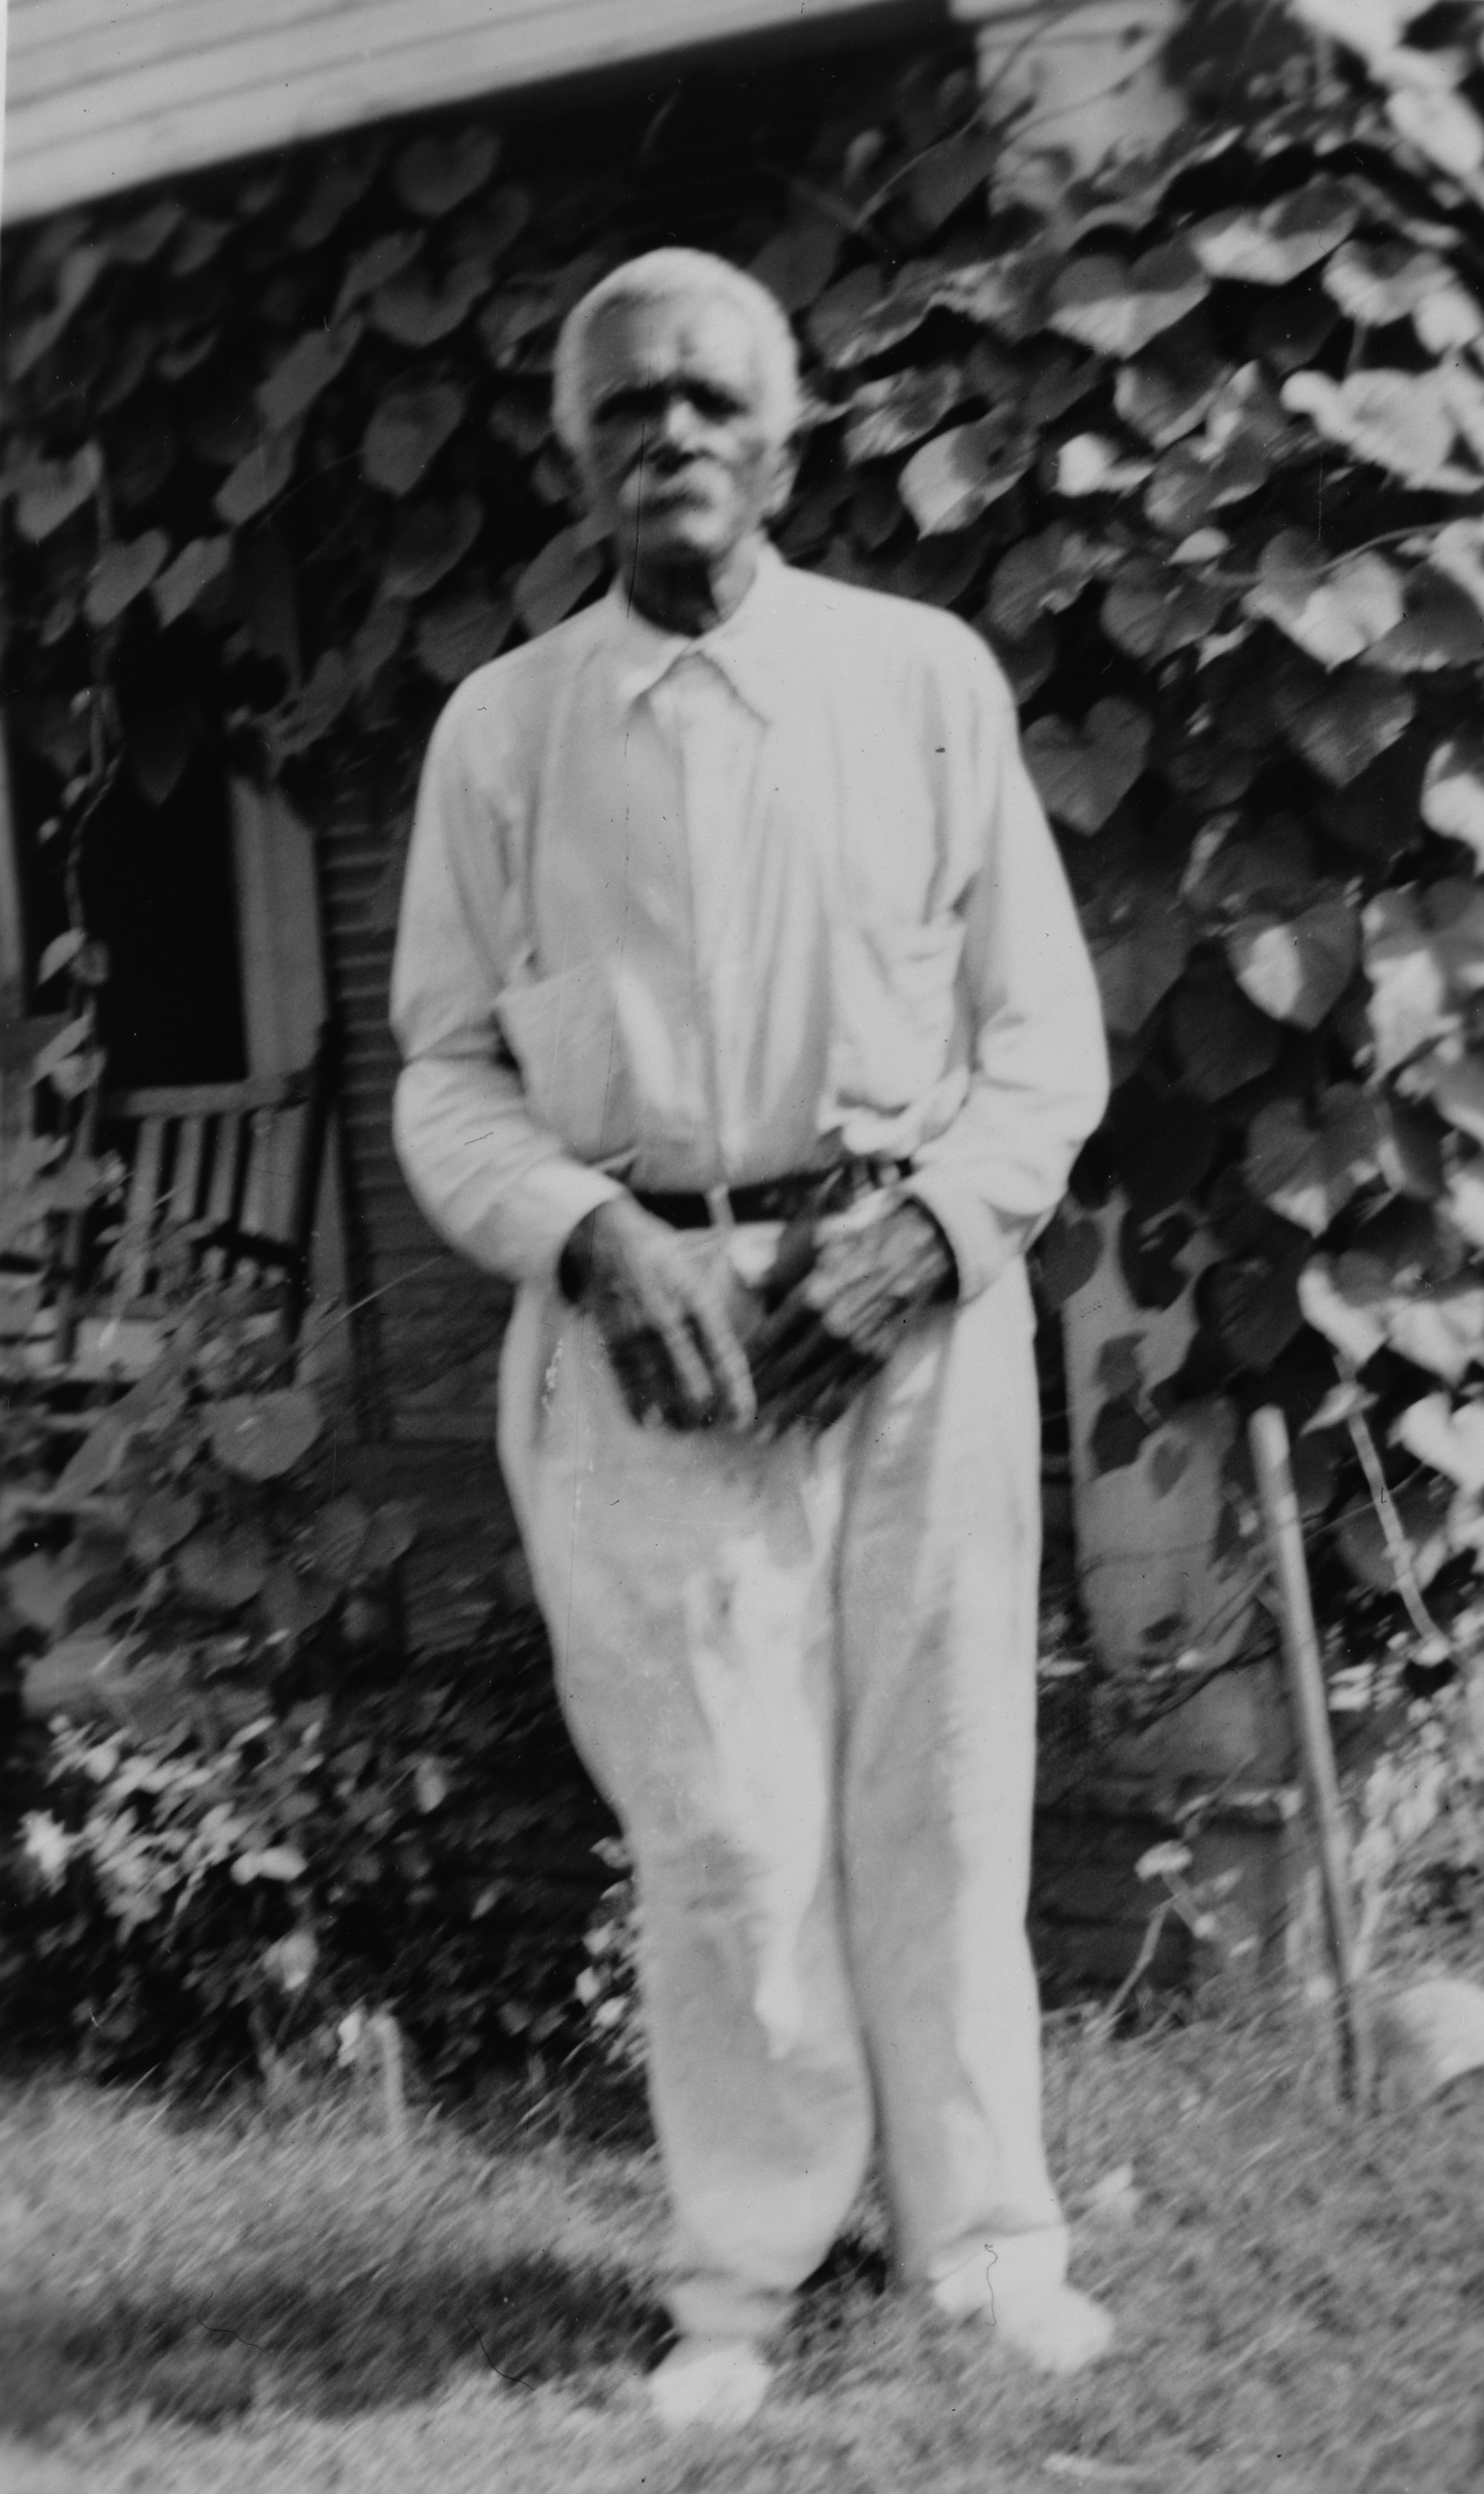
\includegraphics[width=90mm]{./imgs/catocarter_recorte.jpg} \label{img10}
\caption{Cato Carter}
%\end{minipage}
\end{figure}

\subsection{Cato Carter, narrativas do Texas, Parte~I,~páginas~204,~209} \label{ref52}

{[}Viveu em situação de escravidão no Condado de Wilcox, Alabama.{]} ``Vovó era juksie, porque a mãe dela era negra e o pai era um índio
Choctaw. É o que me deixa tão misturada com sangue índio e africano e
branco. Às vezes eu me importava com isso, às vezes não. Não me importo
mais, pois não estou longe do fim dos meus dias.

\textls[-15]{Eu tinha um irmão e uma irmã que ajudei a criar. Os dois eram quase
todos negros. Mas os Carters me disseram para nunca me preocupar com
eles, porque mamãe era do sangue deles e nenhum de nós na nossa família
nunca ia ser vendido, e que um dia iam fazer de nós homens e mulheres
livres. Meu irmão e minha irmã moravam com os negros, no entanto.
(\ldots{})}

Enquanto vivi, segui o que os meus brancos me diziam, exceto uma vez.
Tinha um negro trabalhando no eito que vivia puxando as mulas a
solavancos. O senhor Oll ficou brabo, então me deu uma arma e disse:
`Vai lá e mata aquele homem'. Eu disse: `Senhor Oll, por favor, não me
manda fazer isso. Eu nunca matei ninguém e não quero matar'. Ele
respondeu: `Cato, faz o que estou mandando'. Ele estava falando sério.
Fui até o negro e disse: `Você tem que ir embora neste instante, e eu
também, porque me mandaram matar você, só que eu não vou, então o senhor
Oll vai me matar'. Ele soltou os arreios e nós saímos correndo, se
arrastamos por debaixo da cerca e fugimos''.

\subsection{Savilla Burrell, narrativas da Carolina do Sul, Parte~I,~página~150} \label{ref39}

``Venderam um dos filhos de mamãe uma vez, e quando ela se pôs a chorar
por isso, o senhor disse: `para com essa choradeira se não quiser sentir
o chicote'. Ela chorou e se lamentou a noite inteira. Roupas. Sim,
senhor, nós estávamos sempre meio pelados. Meninos crescidos andavam
descalços e só de camisa o verão inteiro. (\ldots{}) O velho senhor era
o pai de algumas das crianças mulatas. As relações com as mães dessas
crianças era o que dava tanta tristeza para a senhora. Os vizinhos
falavam e ele tirava todas as crianças das mães e vendia para um
traficante. Minha senhora chorava por causa disso''.

\begin{figure}[]
\centering
 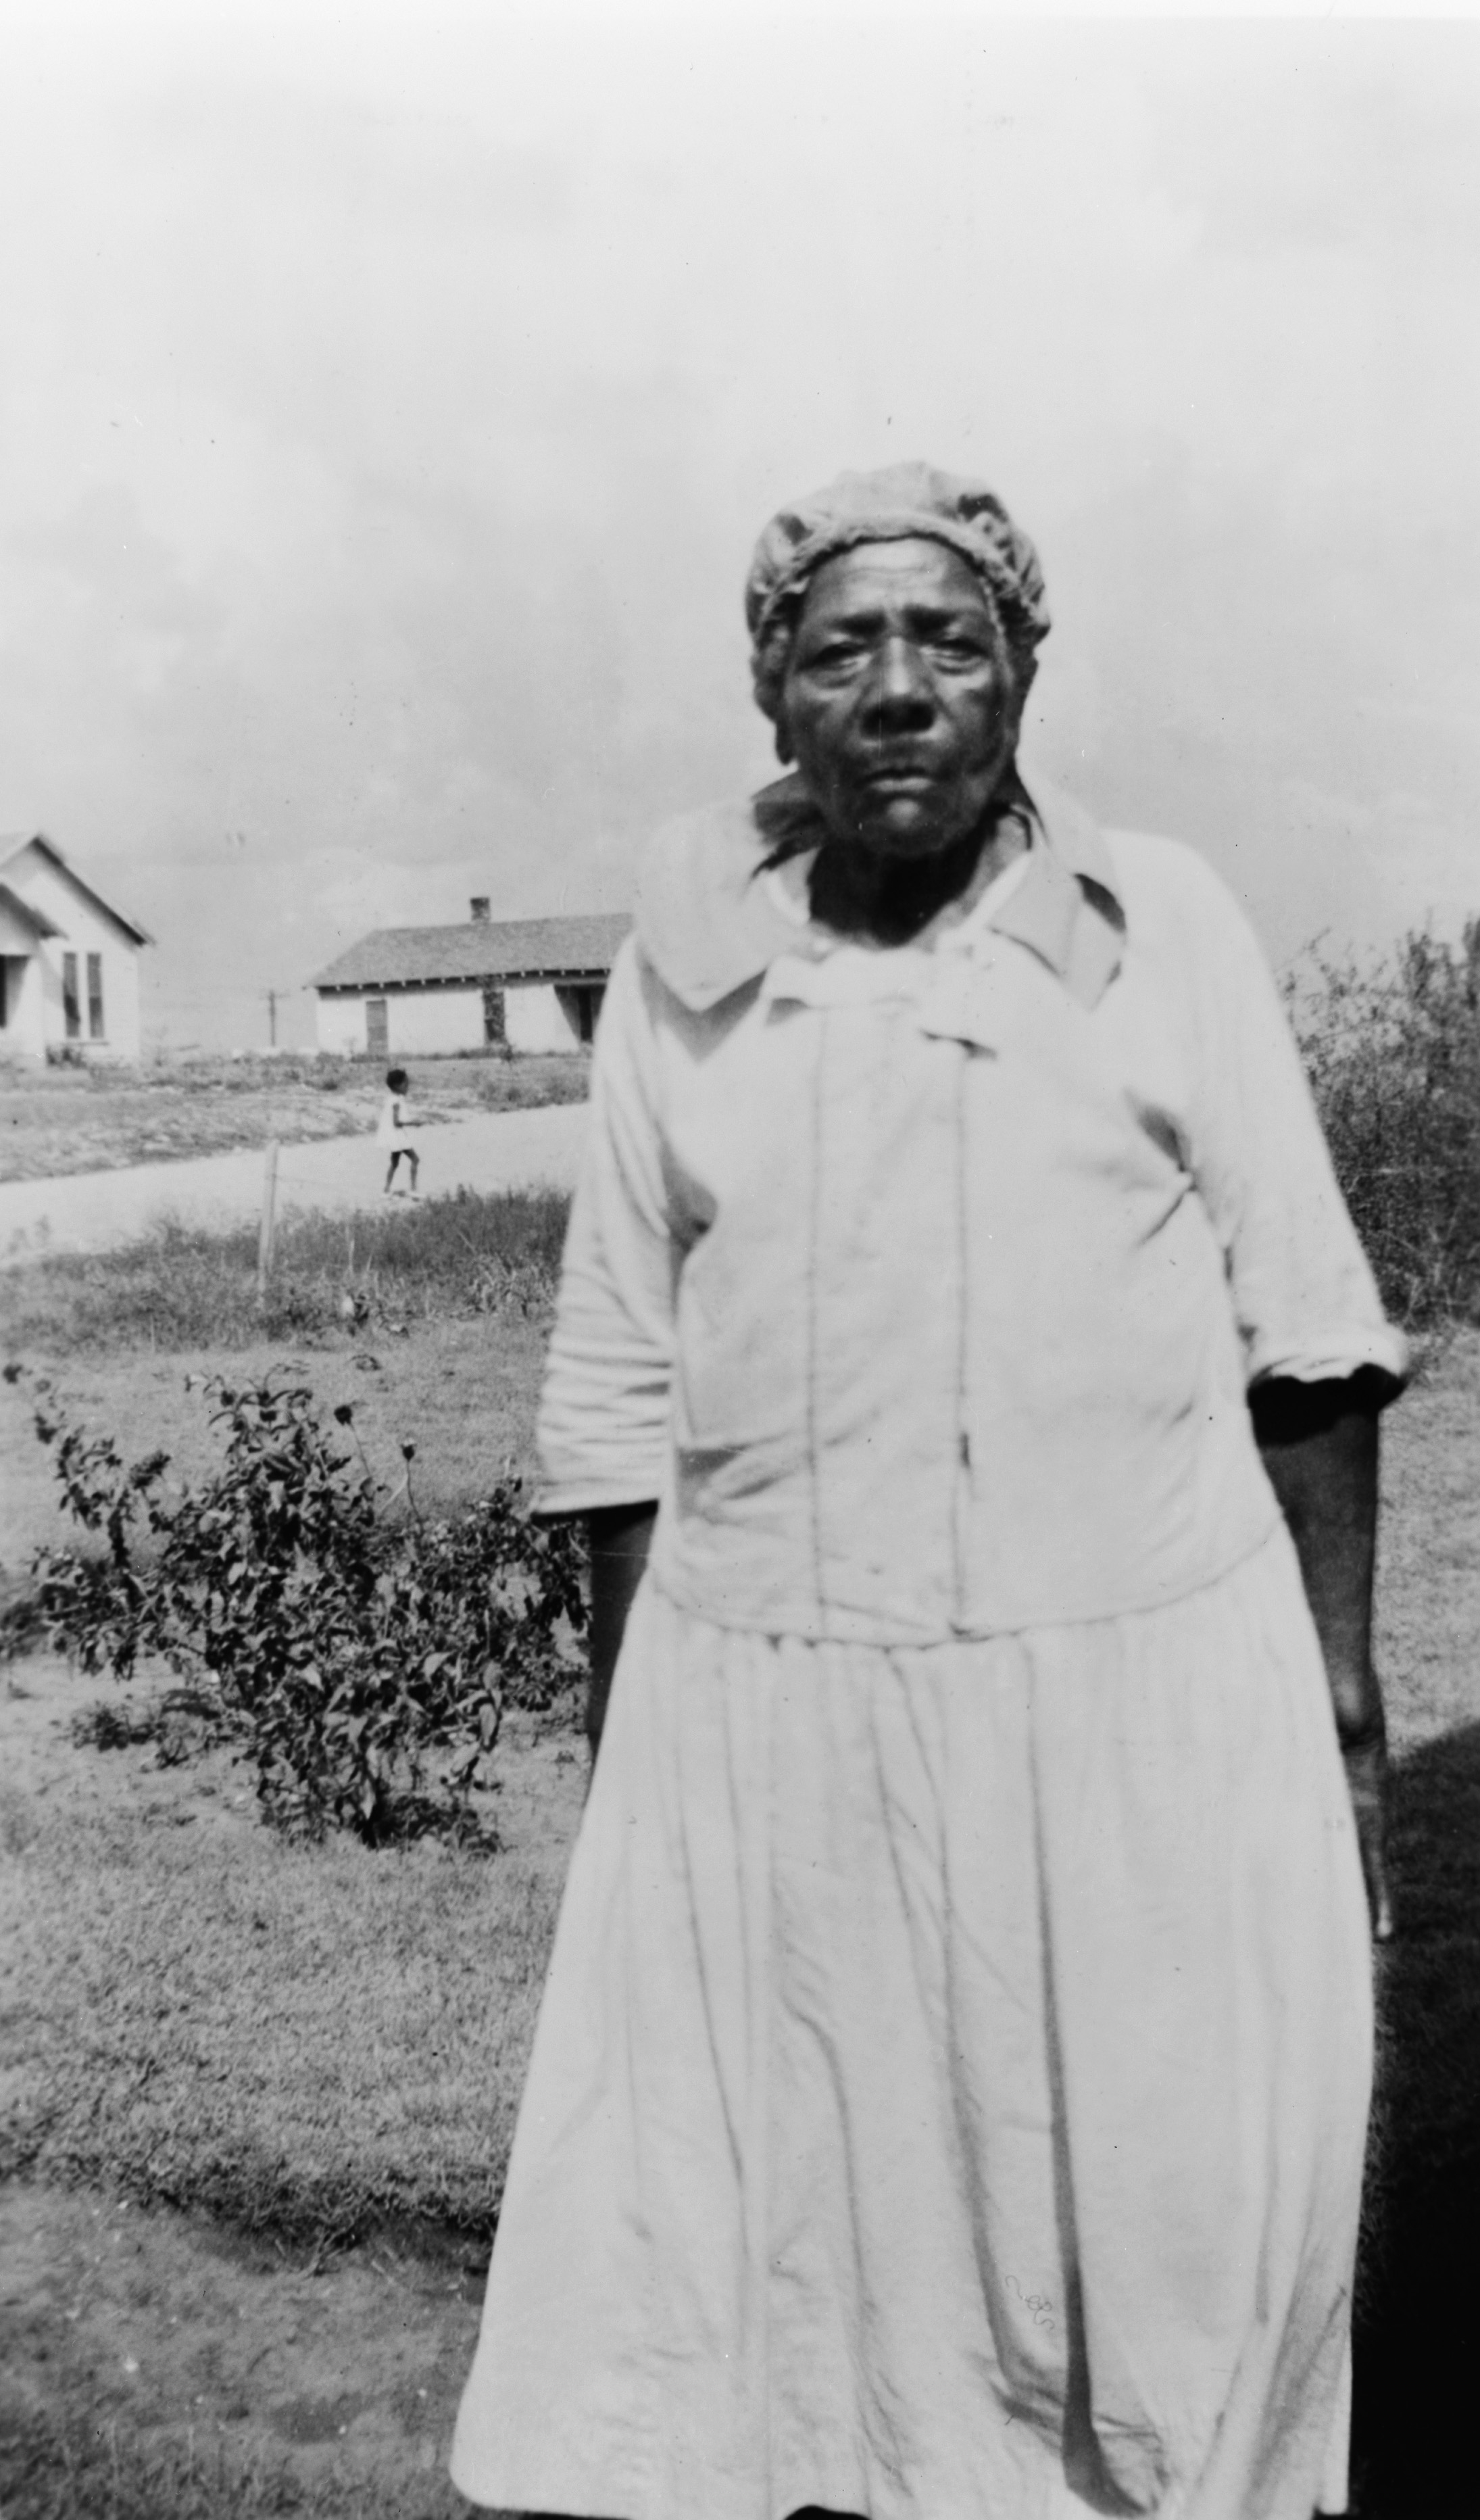
\includegraphics[width=90mm]{./imgs/bettypowers_recorte.jpg} \label{img11}
\caption{Betty Powers}
\end{figure}

\subsection{Betty Powers, narrativas do Texas, Parte~\versal{III},~páginas~191--92}
\label{ref212}

``Se a gente tinha casamentos? Um homem branco como o senhor sabe que
não. Naquela época, os negros só eram juntados. O senhor dizia: `Jim e
Nancy, vocês vão viver juntos', e quando vinha essa ordem, era melhor
obedecer. Na fazenda, não se importavam nada com os sentimentos das
mulheres e não se tinha nenhum respeito por elas. O feitor e os brancos
tiravam vantagem das mulheres como bem entendiam. E as mulheres não
podiam azucrinar ninguém por causa disso. Caso contrário, lá vinha o
chicote para elas. Graças a Deus a rendição chegou antes de eu ser
crescida o suficiente para passar por essas coisas. Sim, senhor, a
rendição salvou esta negra aqui dessas coisas''.

\subsection{Rose Williams, narrativas do Texas, Parte~\versal{IV},~página~177}

{[}Foi escrava de um traficante negreiro, no Condado de Bell,
Texas. Um escravo chamado Rufus, que era um ``valentão'', queria dormir com
ela, ao que resistiu violentamente.{]}

``No dia seguinte, o senhor me chamou e disse: `Mulher, eu paguei um
dinheirão por você foi porque quero ver você com filhos. Coloquei você
para morar com o Rufus para isso. Agora, se não quiser ser açoitada no
pelourinho, faz o que estou mandando'. (\ldots{}) Aí está. O que é que
eu ia fazer? (\ldots{}) Nunca casei, porque uma experiência chega para
esta negra aqui. Depois do que fiz pelo senhor, nunca mais quis nada com
homem nenhum. Deus perdoe esta negra, mas ele vai ter que me dar licença
e pedir para as outras crescerem e multiplicarem''.

\subsection{Sam Jones Washington, narrativas do Texas, Parte~\versal{IV},~página~138}
\label{ref281}

{[}Viveu em situação de escravidão no Condado de Wharton, Texas.{]} ``O senhor Young tinha uma fazendinha junto ao rio Colorado e não tinha
muitos escravos. Era mamãe e os seus seis filhos e Marjoria com seus
quatro. Papai não era de lá. Chamavam ele para o serviço e, quando
tinham o que queriam, ele voltava para o senhor dele. As mulheres na
fazenda do senhor Young não eram casadas''.

\subsection{Henry Nelson, narrativas do Arkansas, Parte~V,~página~198}

{[}Viveu em situação de escravidão no Condado de Crittenden, Arkansas.{]} ``Minha mãe e meu pai não tiveram educação. (\ldots{})

Ela não morou com o primeiro marido depois da escravidão, deixou dele
quando foi libertada. Ela nunca quis casar com ele, foi forçada a isso''.

\subsection{Fred Brown, narrativas do Texas, Parte~I,~página~158} \label{ref36}

{[}Viveu em situação de escravidão na Paróquia de Baton Rouge, Luisiana.{]} ``Às vezes o feitor não deixava eles casarem. Deixa eu explicar. O
trabalho dele também era ser pai das crianças. Ele escolhia as mulheres
parrudas e saudáveis, que iam ter filhos parrudos também. O feitor era
um homem parrudo. Quem ele escolhia ele mandava, e não deixava casar nem
andar com os outros negros. Se andavam, era chicote na certa. O senhor
criou umas crianças bem parrudas e bonitas, e vendeu algumas depois de
crescerem um pouco, por 500 dólares ou até mais''.

\paragraph{Comentário}\quad
{\small
Após a Guerra Civil, quando conquistaram a sua
liberdade, milhares de negros fizeram esforços incríveis e emocionantes para se
reunir com familiares perdidos havia muitos anos. Hoje, é difícil
imaginar os obstáculos que enfrentavam ou a determinação com a qual
conduziam suas buscas. Muitos fizeram longas jornadas a pé, sabendo
quase nada onde seus maridos, mulheres ou filhos poderiam estar. Para
obter informações, tudo que podiam fazer era perguntar a outros negros
se haviam ouvido falar sobre um indivíduo, ou uma família, ou um
determinado proprietário. Muitas dessas buscas com certeza foram em vão,
mas as narrativas, assim como outras fontes, indicam que, de alguma
forma, muitos conseguiram reencontrar seus entes
queridos.\footnote{Heather Andrea Williams, \emph{Help Me to Find My
  People: The African American Search for Family Lost in Slavery}
  (Chapel Hill: The University of North Carolina Press, 2012).}
}

\begin{figure}[]
\centering
 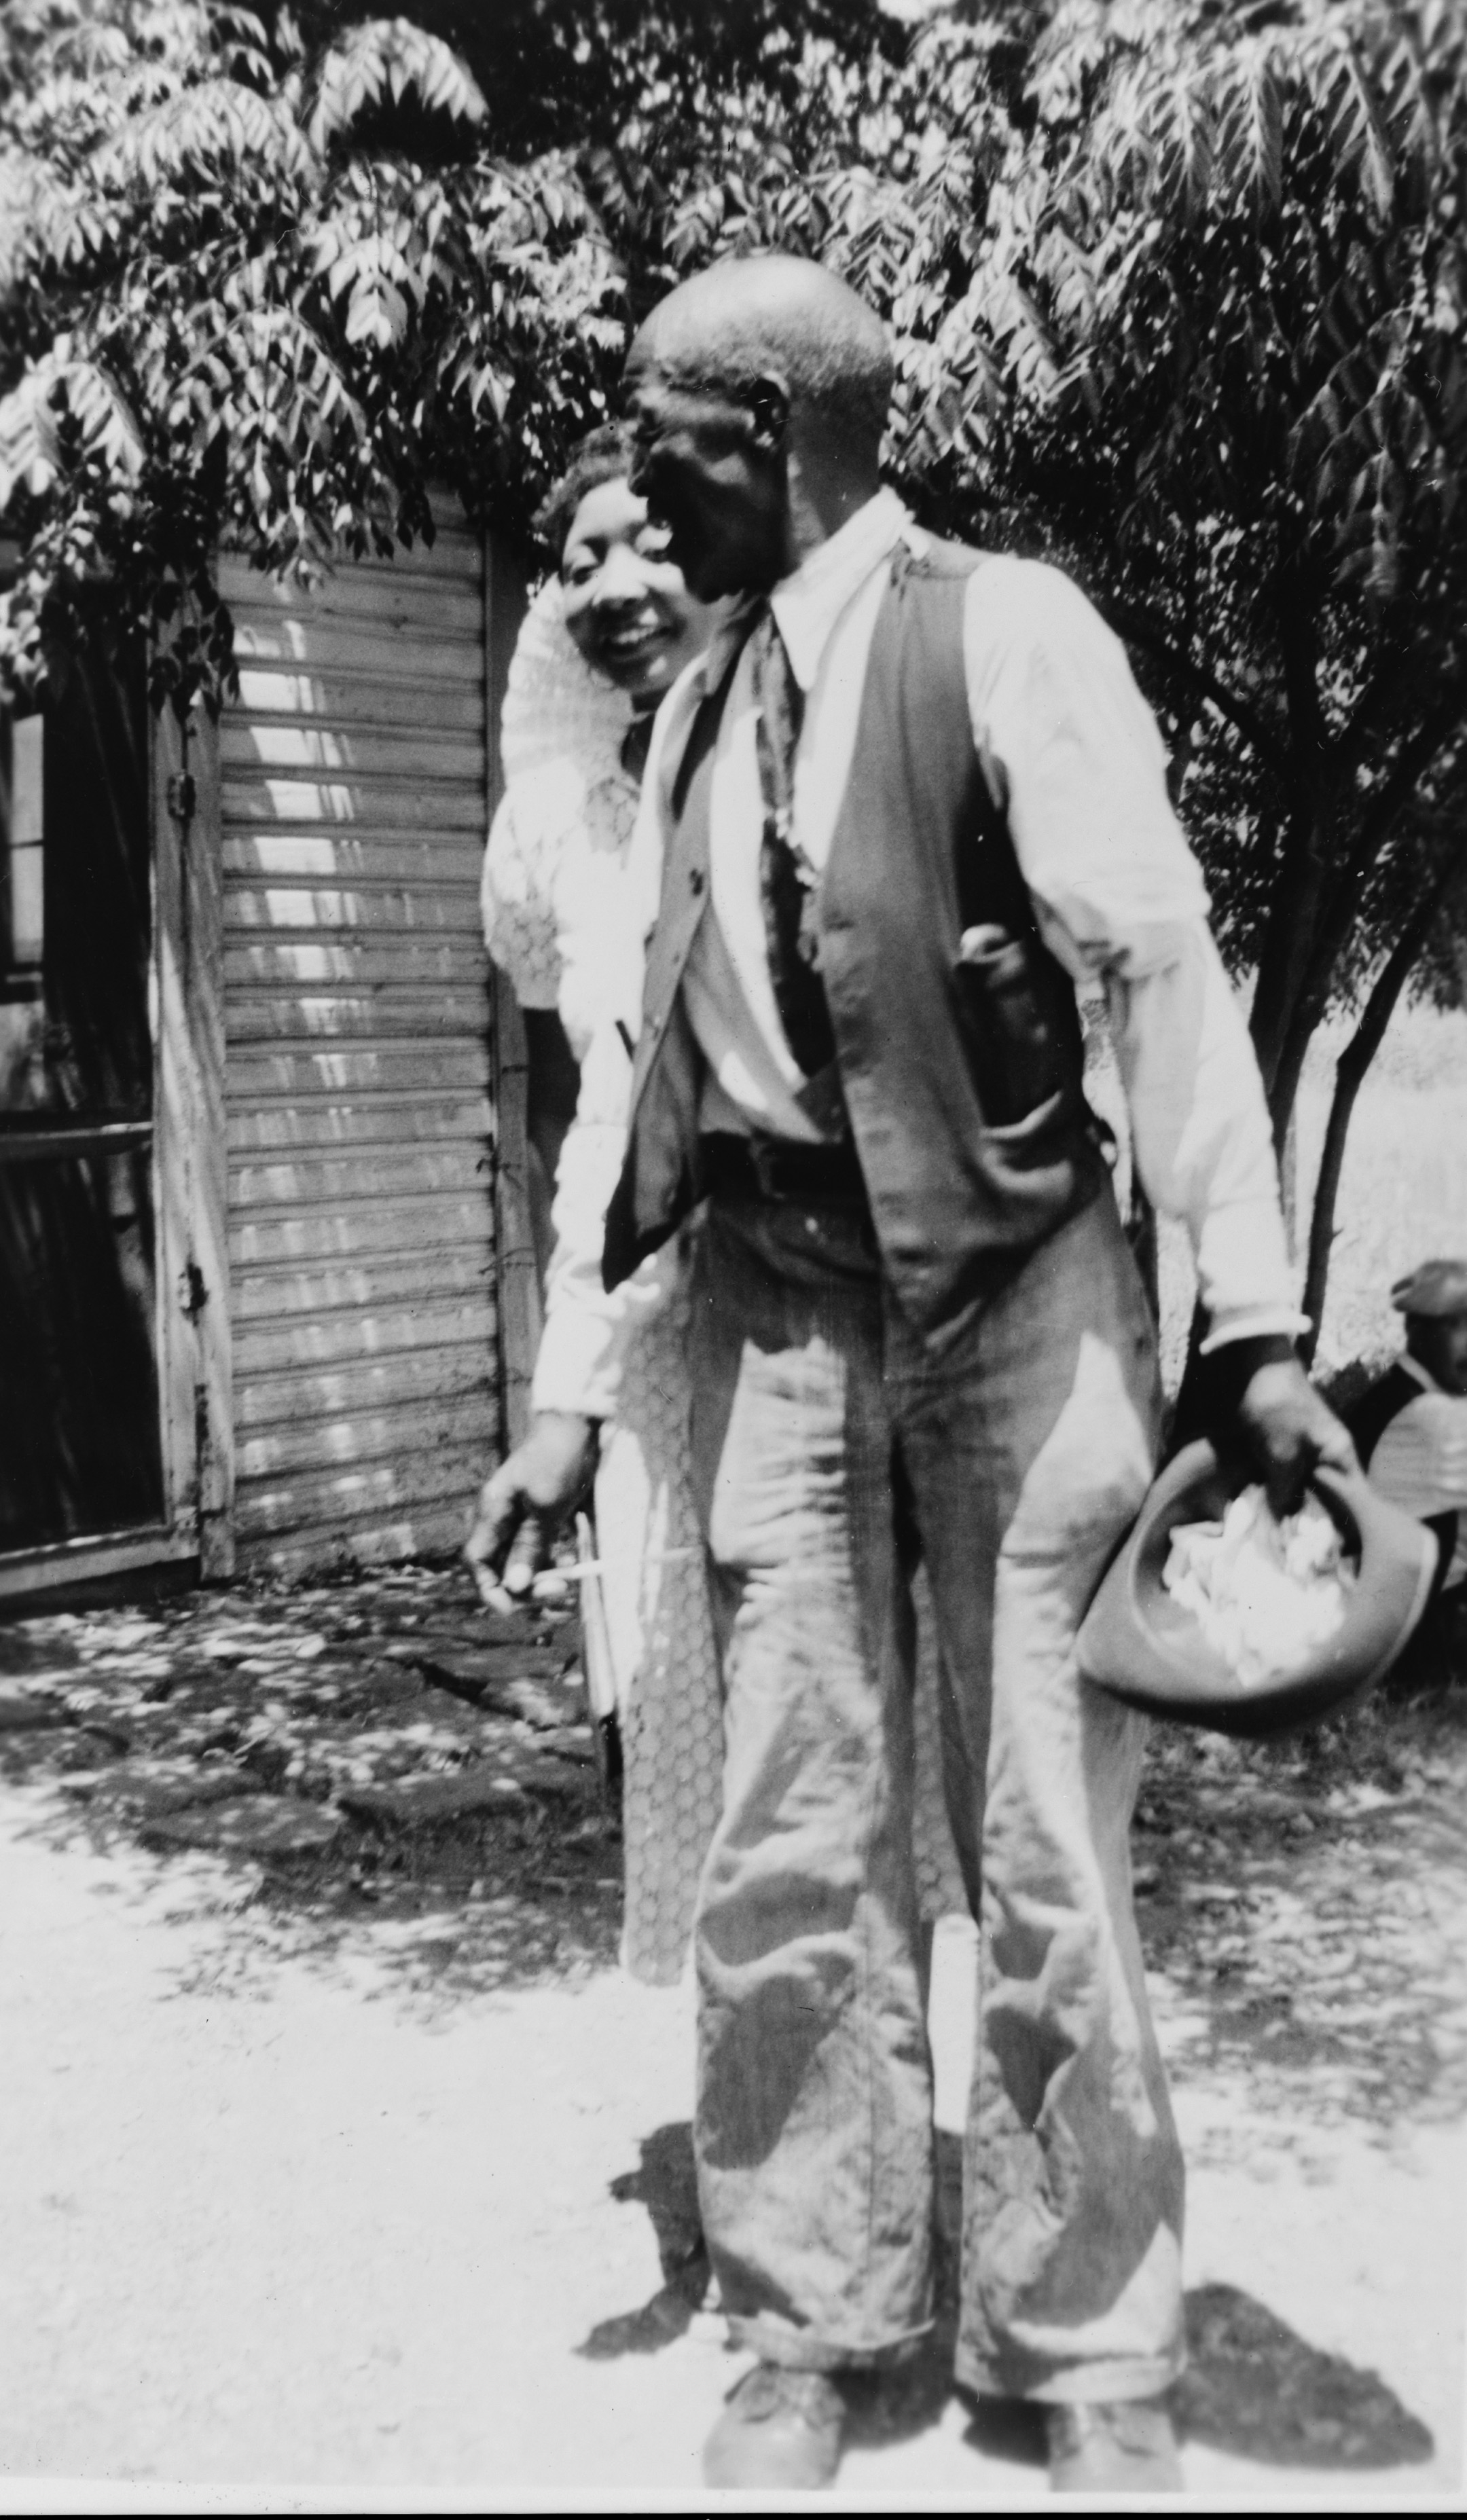
\includegraphics[width=90mm]{./imgs/fredbrown_recorte.jpg} \label{img12}
\caption{Fred Brown}
\end{figure}

\subsection{Nettie Henry, narrativas do Mississippi, páginas 61--62}
\label{ref142}

``Papai não foi conosco para Meridian. Ele pertencia a um grupo de
brancos, sabe, e mamãe pertencia a outro. Ele vinha nos ver até a guerra
começar, mas depois a gente dele se foi para o Texas (\ldots{}) e levou
papai com eles. Mas depois da guerra ele voltou para nós, caminhou quase
todo o caminho desde lá do Texas''.

\subsection{George Lewis, narrativas da Geórgia, Parte~\versal{III},~página~50}
\label{ref173}

{[}Viveu em situação de escravidão em Pensacola, Flórida. Seu pai pertencia a um proprietário e o resto da família a uma pessoa diferente, que se mudou da Flórida para a Geórgia.{]} ``Vários meses
depois que a liberdade foi declarada, o pai do Sr. Lewis conseguiu se
reunir com a família, que ele não via desde a mudança para a Geórgia''.

\subsection{John N. Davenport, narrativas da Carolina do Sul, Parte~I,~página~242} \label{ref66}

``Quando a liberdade chegou, o senhor disse que a gente poderia ir
embora ou ficar. A maioria ficou com ele. Logo depois, ele ficou brabo
comigo um dia e me mandou ir embora da fazenda. Eu vim para a cidade e
fiquei umas duas semanas vagabundeando. Descobri onde estava minha mãe,
que tinha sido vendida. Ela estava em Saluda (Cidade Velha). Fui até ela
e fiquei duas semanas, depois ela veio para Newberry e alugou um casebre
no Riacho Beaver Dam, perto da Rua Silver''.


\pagebreak
\thispagestyle{empty}
\movetoevenpage
\thispagestyle{empty}

\begin{absolutelynopagebreak}
\begin{vplace}
\begin{figure}[H]
\begin{adjustwidth}{-1.8cm}{}
  %\centering
  \vspace*{-2cm}
  %\hspace{-0.5cm}
  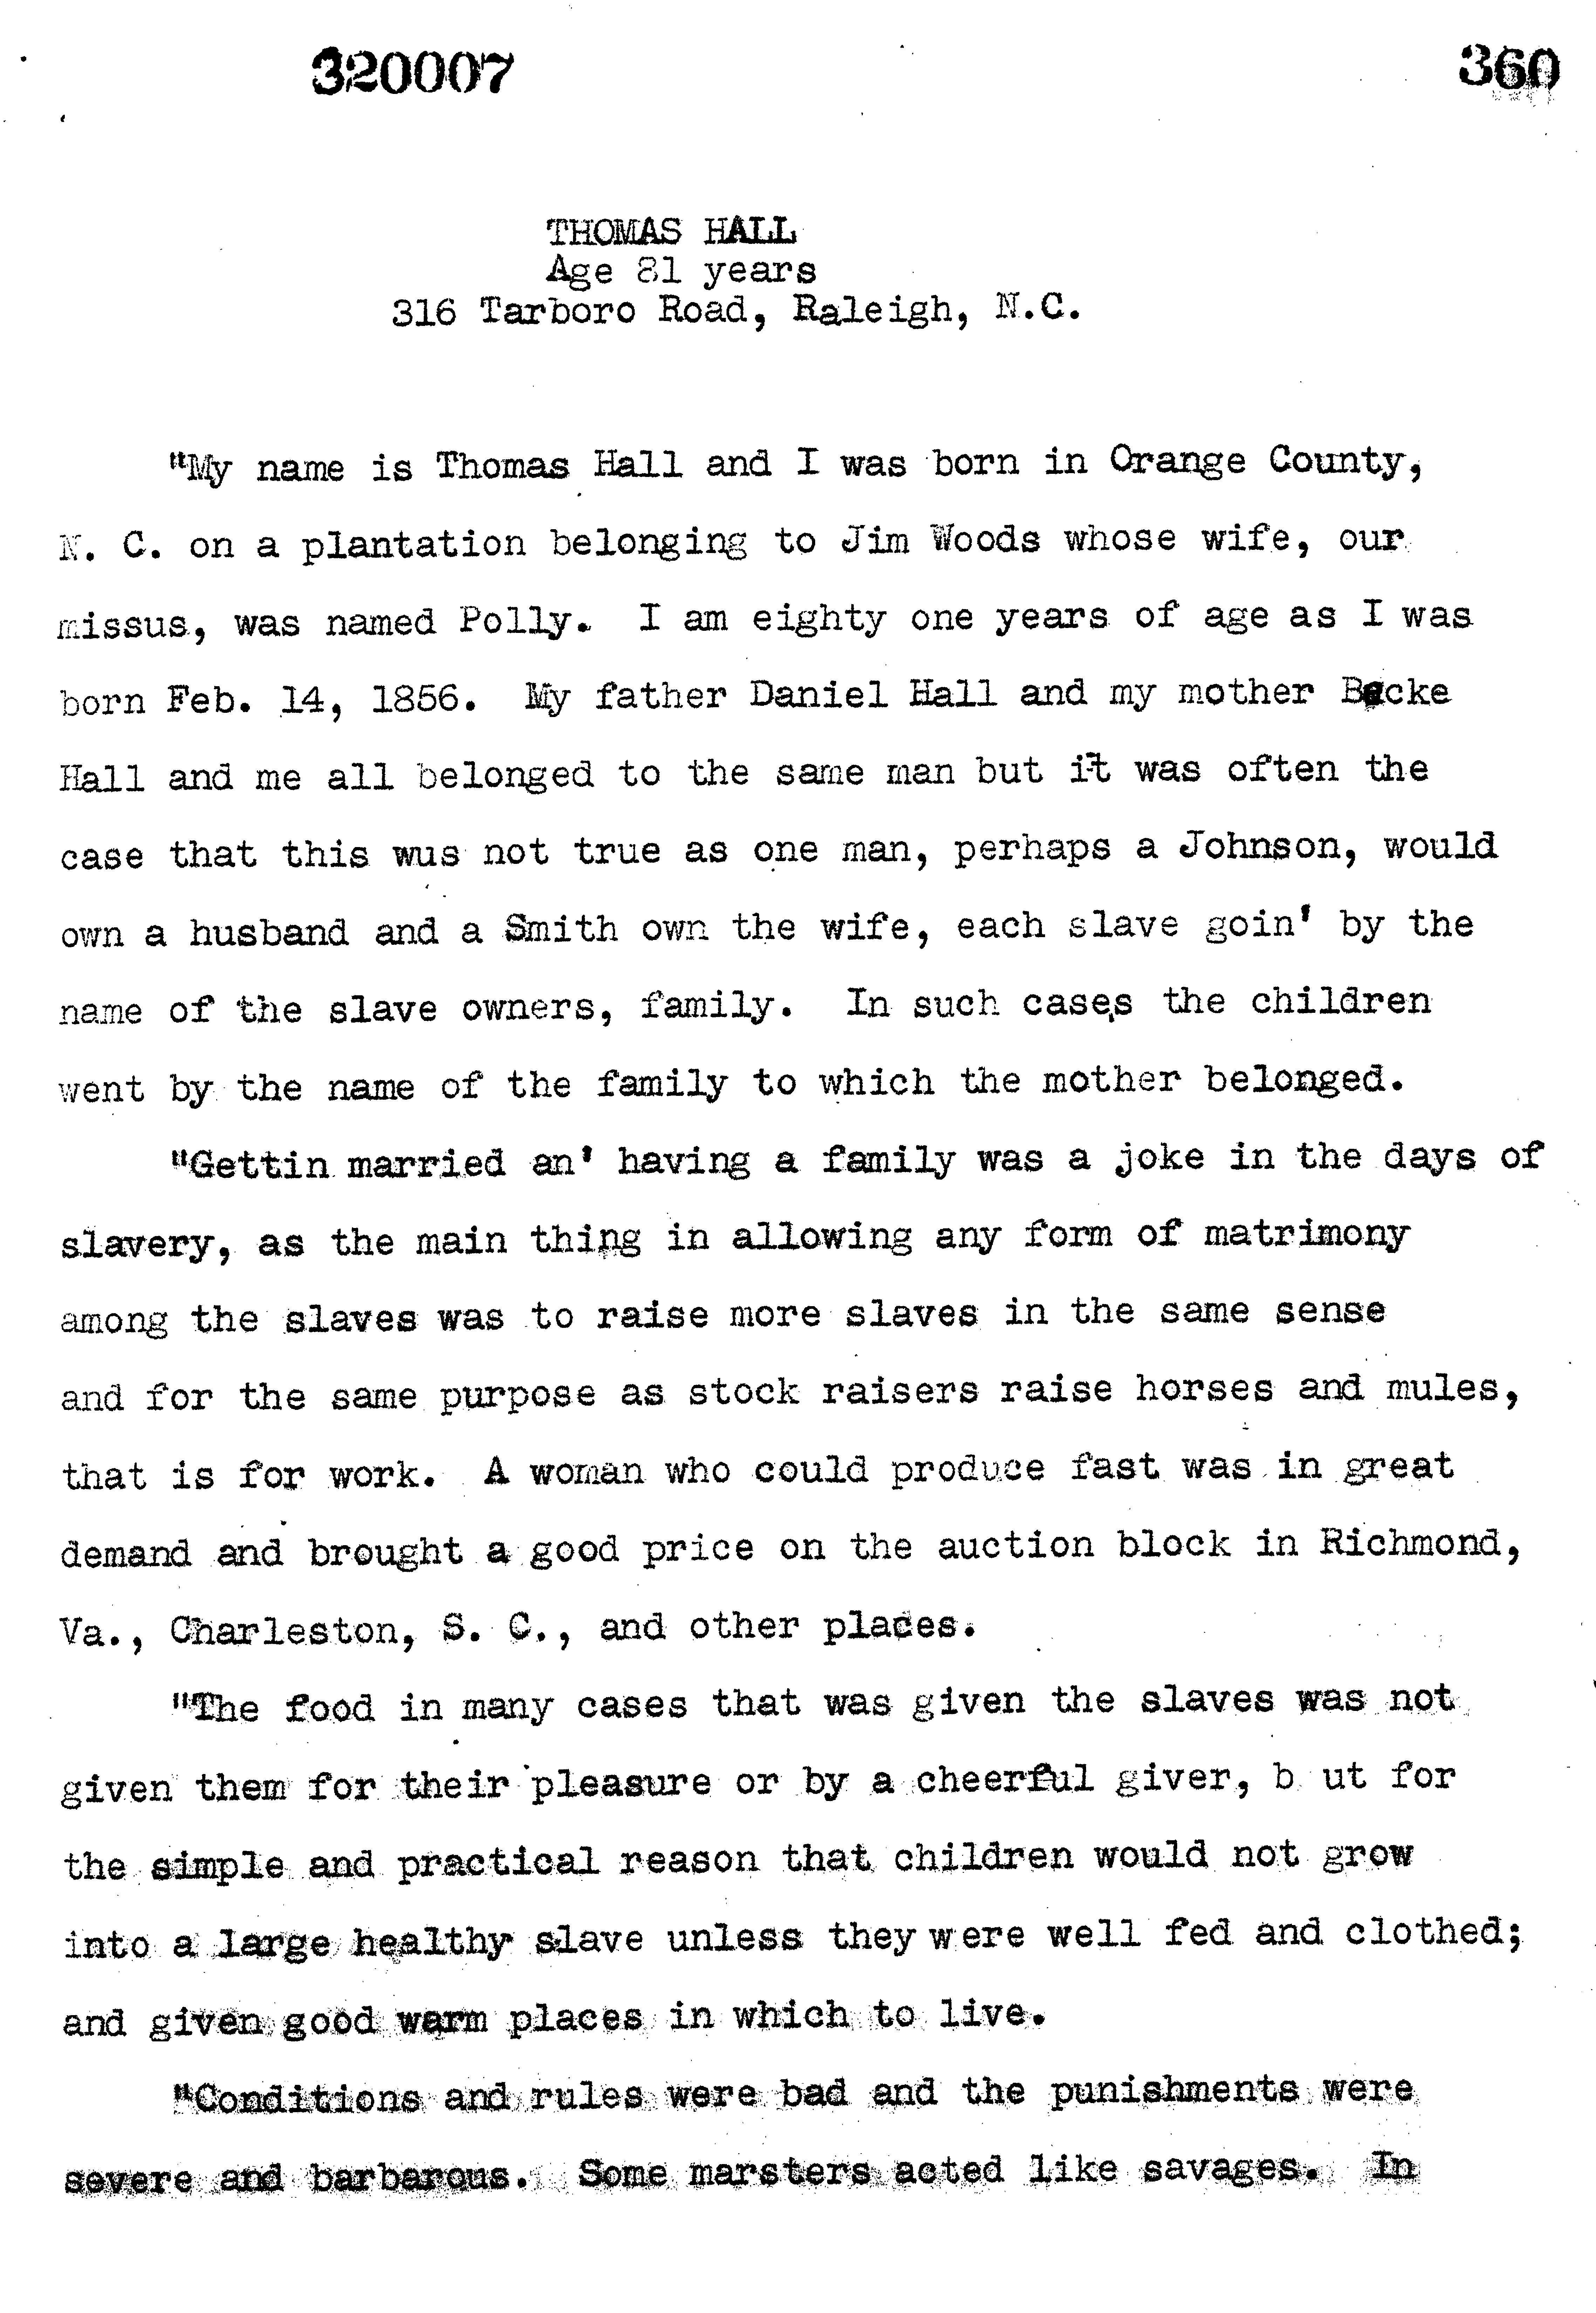
\includegraphics[width=130mm]{./imgs/Cap5.jpg}  
  %\hfill
\end{adjustwidth}
  \caption{Thomas Hall, narrativas da Carolina do Norte, Parte \versal{I}, página 360}
\end{figure}
\end{vplace}

\end{absolutelynopagebreak}

\chapter{Atitudes raciais}
%\addcontentsline{toc}{chapter}{{\large\versal{V.}} Atividades raciais}
%\hedramarkboth{Atitudes raciais}{}

\subsection{Thomas Hall, narrativas da Carolina do Norte, Parte~I,~páginas~360--62}
\label{ref118}

``Meu nome é Thomas Hall e eu nasci no Condado de Orange, Carolina do
Norte, em uma fazenda pertencente a Jim Woods, cuja esposa, nossa
senhora, se chamava Polly. Tenho 81 anos de idade, pois nasci em 14 de
fevereiro de 1856. Meu pai, Daniel Hall, minha mãe, Becke Hall, e eu
todos pertencíamos ao mesmo homem, mas muitas vezes isso não acontecia,
pois um homem, por exemplo, um Johnson, seria dono do marido, enquanto
um Smith seria dono da esposa, com cada escravo usando o nome da família
do senhor de escravos. Nesses casos, os filhos levavam o nome da família
à qual a mãe pertencia.

Casar e formar família era uma piada nos tempos da escravidão, pois o
principal objetivo por trás de permitir qualquer forma de matrimônio
entre os escravos era criar mais escravos, no mesmo sentido e para os
mesmos fins que os pecuaristas criam cavalos e mulas, ou seja, para
trabalhar. A procura era forte por uma mulher capaz de se reproduzir com
rapidez e ela rendia um bom preço nos leilões de Richmond, Virgínia,
Charleston, Carolina do Sul, e outros lugares.

Em muitos casos, a comida que era dada aos escravos não lhes era dada
para o seu prazer ou por uma mão alegre, mas pelo motivo simples e
prático que as crianças não cresciam e se tornavam escravos grandes e
saudáveis se não fossem bem alimentadas e vestidas e se não pudessem se
abrigar do frio nas suas moradias.

As condições e as regras eram ruins e os castigos eram severos e
bárbaros. Alguns senhores agiam feito selvagens. Em alguns casos, os
escravos eram queimados na fogueira. As famílias eram separadas pelas
vendas. As mães eram vendidas dos filhos. Os filhos eram vendidos das
mães e o pai não era considerado minimamente parte da família. Essas
condições existiam antes da Guerra Civil e as condições, ainda que
alteradas, continuam desde então. Os brancos sempre mantiveram os
escravos em semiescravidão e ainda praticam as mesmas coisas com eles de
formas diferentes. Os brancos ainda lincham, queimam e perseguem a raça
negra na América e há pouco que estejam fazendo para ajudá"-la.

Lincoln levou a fama por nos libertar, mas foi o que ele fez? Ele nos
deu liberdade sem nos dar a chance de viver por conta e ainda
precisávamos depender dos brancos sulistas para trabalho, comida e
vestuário, e eles usaram nossa necessidade e privação para nos manter em
um estado de servidão quase nada melhor do que a escravidão. Lincoln não
fez quase nada pela raça negra, e nada do ponto de vista dos vivos. Os
brancos não vão fazer nada pelos negros além mantê"-los subjugados.

Harriet Beecher Stowe, a escritora da \emph{Cabana do pai Tomás}, fez
isso por si mesma. Ela tinha os seus próprios interesses e eu não gosto
dela, do Lincoln, de ninguém daquela turma. Os yankees ajudaram a nos
libertar, ou assim dizem, mas eles deixaram nos jogar de volta na
escravidão.

Quando penso na escravidão, fico furioso. Não acredito em lhe contar a
minha história, porque apesar de todas as promessas que fizeram, os
negros ainda estão em más condições nos Estados Unidos. Não importa onde
ele mora, é tudo igual. Você pode ser bom, alguns homens brancos são,
mas a pressão dos seus amigos brancos é tal que você vai ser forçado a
falar mal de nós e virar a cara para nós quando estiver ao redor deles,
mesmo que goste de nós no fundo do coração.

Você está andando por aí para ouvir a história das condições da
escravidão e as perseguições dos negros antes da Guerra Civil e as
condições econômicas deles desde a guerra. Após tanto tempo, você já
devia saber isso tudo. Você vai nos ajudar? Não! Vai só ajudar a si
mesmo. Você diz que a minha história pode aparecer em um livro, que é do
Projeto Federal de Escritores. Harriet Beecher Stowe escreveu \emph{A
cabana do pai Tomás}. Não gostei do livro e odeio ela. Não me importa de
onde você é, não quero que escreva a minha história porque os brancos
foram, são hoje e sempre vão ser contra os negros''.

\paragraph{Comentário}\quad
{\small
A escravidão era coerção e exploração, e também um sistema de
exploração de base racial. Todos os cativos nos Estados Unidos eram
negros, e quase todos os negros no Sul em 1860 (94\%) eram cativos. As
atitudes racistas da supremacia branca sustentavam e apoiavam a
instituição da escravidão e, na sociedade como um todo, consignavam
todos os afro"-americanos, mesmo a pequena minoria em liberdade, a um
estado de subordinação rígida. Os escravizados encontravam o racismo em
todos os dias da sua vida. Era parte essencial do ser escravizado ou
afro"-americano nos Estados Unidos. Assim, não surpreende que a raça era
uma parte fundamental da sua identidade ou que muitos desenvolveram
atitudes raciais fortemente hostis aos brancos.

Contudo, as histórias dos ex"-escravizados também mostram que eles
sabiam distinguir entre os indivíduos e reconhecer a bondade ou
compaixão, fosse ela genuína ou parcial e limitada pela perspectiva dos
brancos. Essa capacidade ajuda a explicar os muitos comentários
positivos sobre senhores de escravos. Os entrevistadores brancos do \versal{FWP}
também sinalizavam as suas expectativas quando pediam aos entrevistados
para falar sobre ``os bons tempos''. As exigências da etiqueta racial no
Sul segregacionista da década de 1930, aliada à lembrança de ter comida
o suficiente sob a escravidão, influenciou o modo como alguns
falaram sobre seus senhores. Mesmo assim, sua consciência e
ressentimento em relação ao racismo ainda transparecia.
}

\begin{figure}[]
%\begin{minipage}{0,4\textwidth}
\centering
 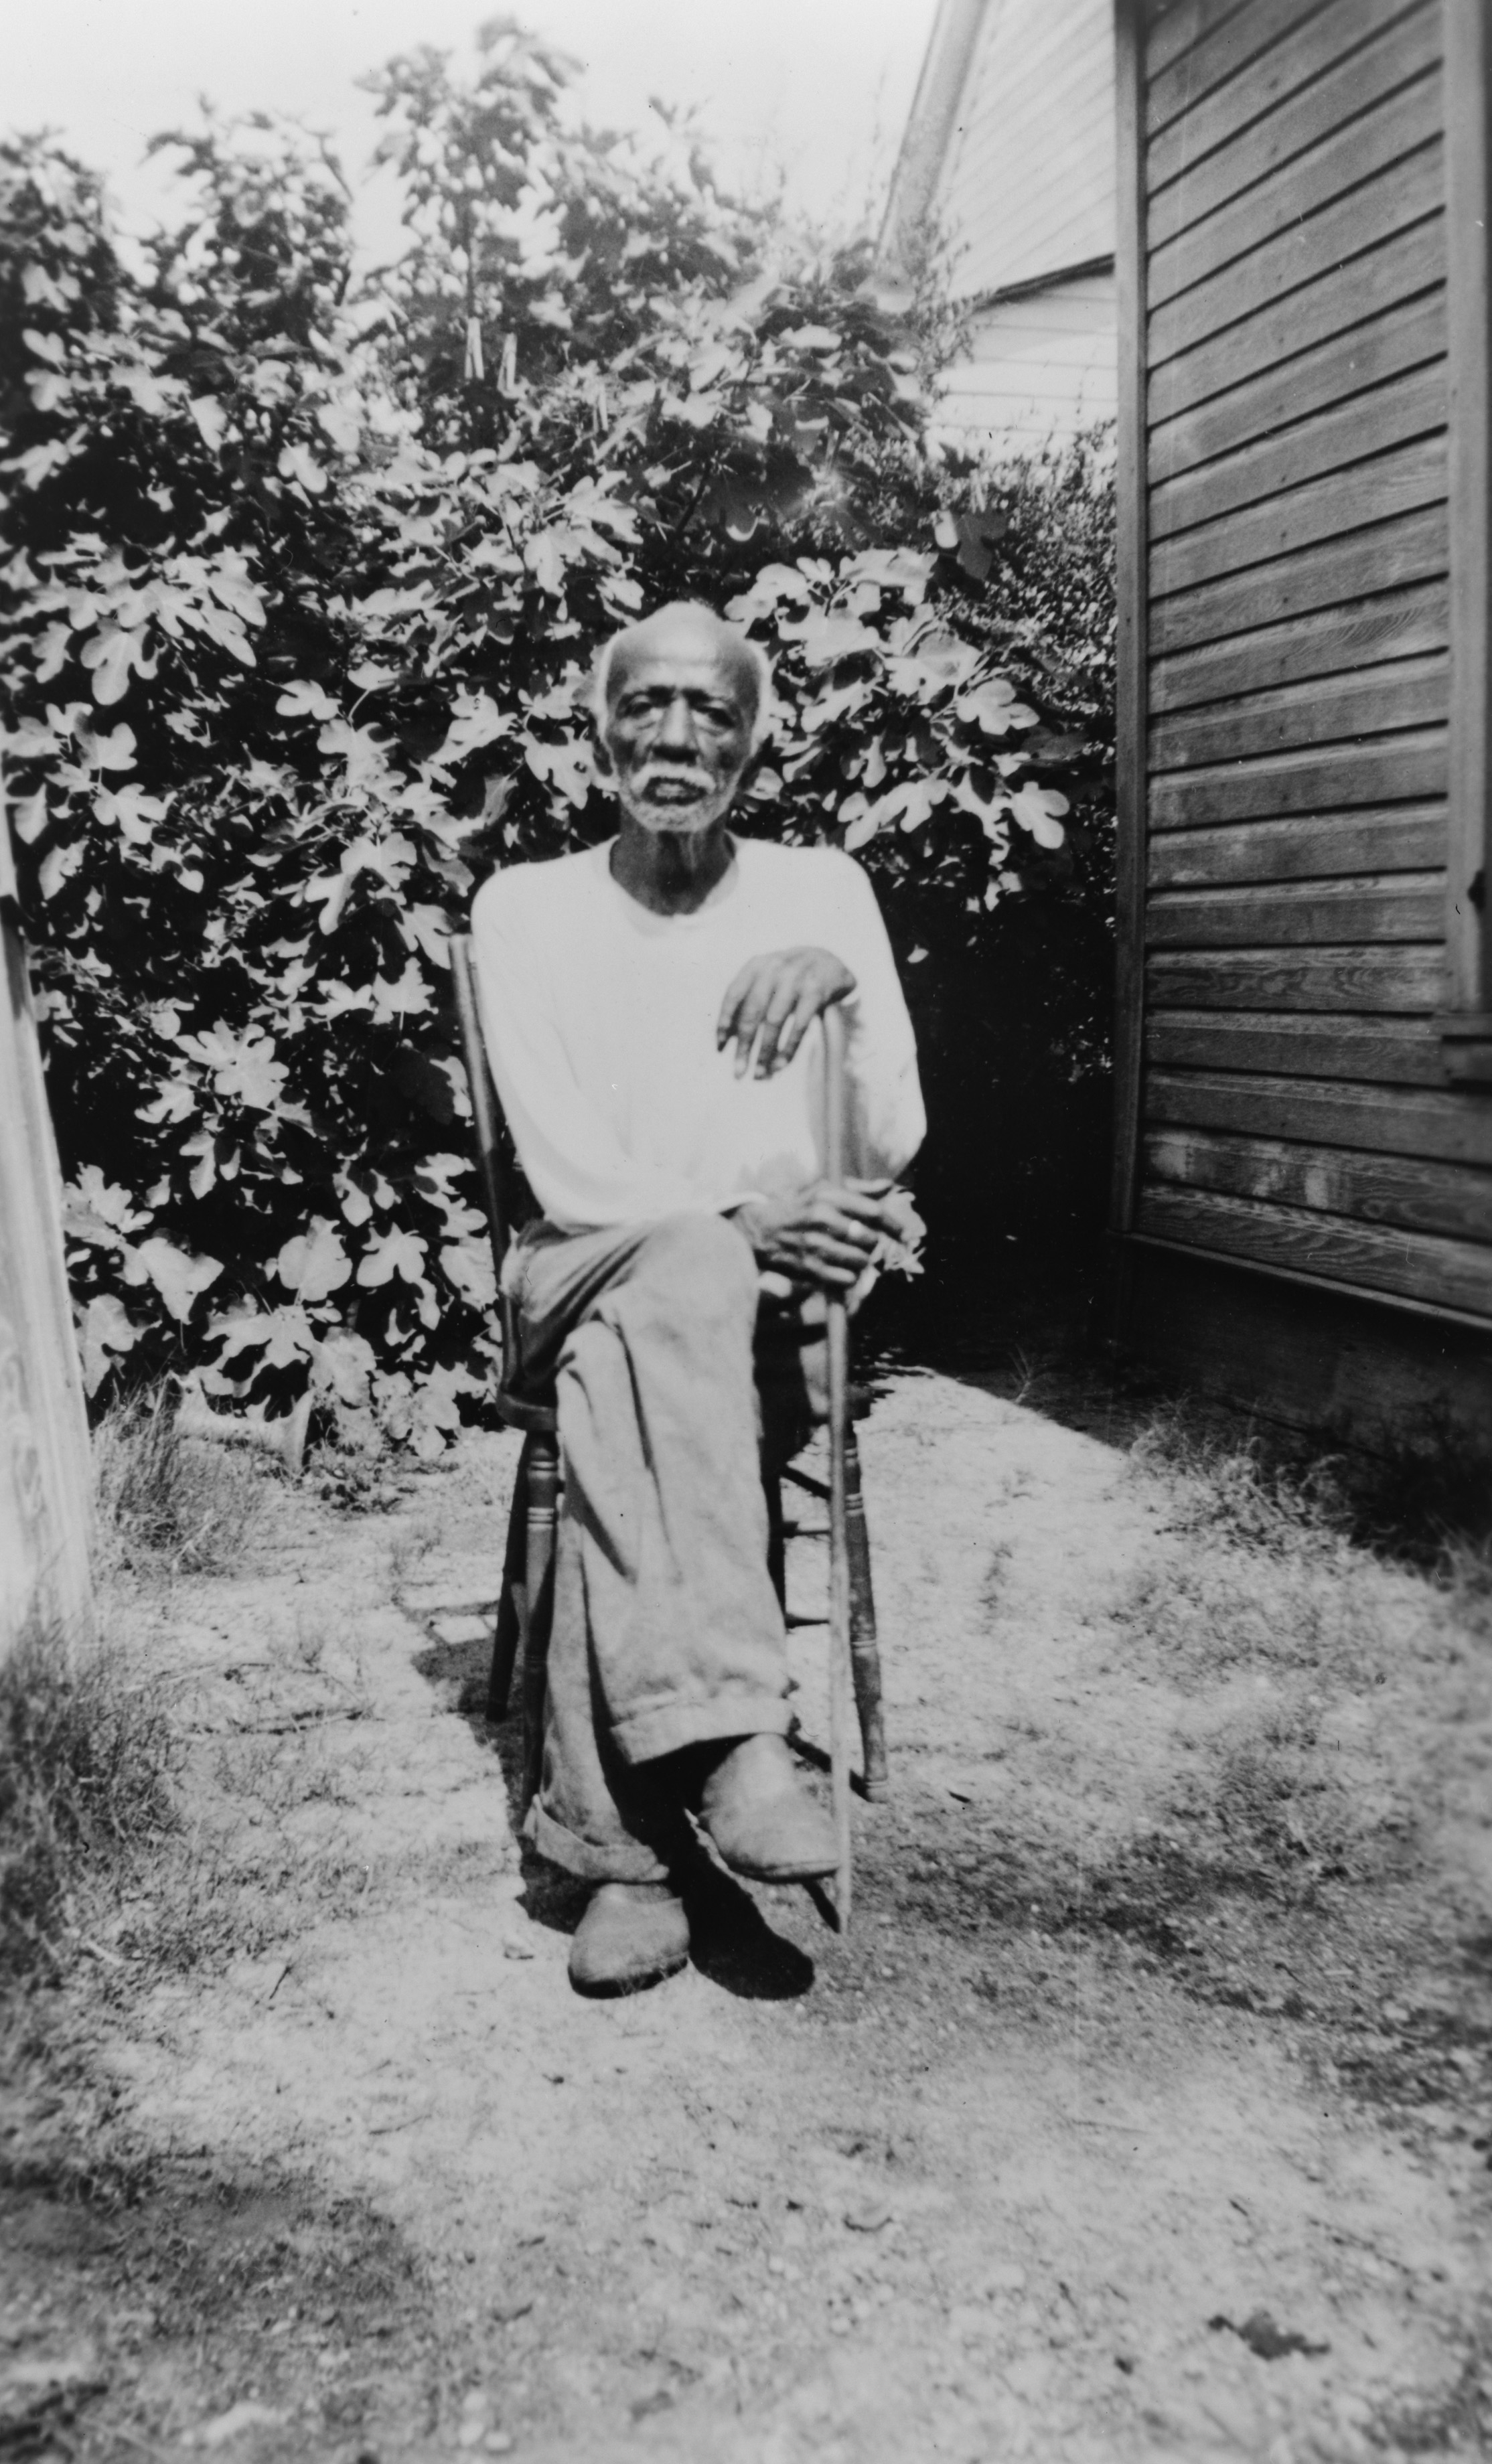
\includegraphics[width=90mm]{./imgs/martinjackson_recorte.jpg} \label{img13}
\caption{Martin Jackson}
%\end{minipage}
\end{figure}

\subsection{Martin Jackson, narrativas do Texas, Parte~\versal{II},~página~189}
\label{ref161}

``Muitos dos velhos escravos fecham a porta antes de contarem a verdade
sobre os dias da escravidão. Quando a porta está aberta, eles contam
sobre como seus senhores eram bondosos e como tudo era idílico. Não se
pode culpá"-los por isso, pois não lhes faltou disciplina na juventude
para ensiná"-los cautela sobre dizer algo que não fosse lisonjeiro sobre
os seus senhores. Eu próprio estava em uma situação um tanto diferente
da maioria dos escravos e, por consequência, não tenho rancores nem
ressentimento. Contudo, posso lhe contar que a vida do escravo médio não
era nada cor"-de"-rosa. Era um sofrimento cruel.

Mesmo com o meu bom tratamento, passei a maior parte do meu tempo
planejando e pensando em fugir. Teria sido fácil para mim, mas meu velho
pai dizia: `Não adianta correr do ruim para o pior à caça do melhor'.
Muitos meninos negros fugiram e se alistaram no exército da União, e
muitos deles recebem pensão até hoje. Meu pai sempre me aconselhava:
`Todo homem tem que servir a Deus debaixo da sua videira, e debaixo da
sua figueira'. Ele sempre lembrava que a guerra não iria durar para
sempre e que a nossa eternidade seria passada entre os sulistas depois
que eles fossem vencidos''.

{[}Martin Jackson foi para a guerra com seu jovem senhor. Ele conta:{]}
``Bem quais eram meus sentimentos sobre a guerra, eu mesmo nunca soube
resolver. Eu sabia que os yankees iam ganhar, desde o início. Eu queria
ver eles ganharem de nós do Sul, mas tinha esperança que iam conseguir
sem precisarem dizimar a nossa companhia {[}a unidade militar na qual
ele e seu senhor serviam{]}''.


\subsection{Elisabeth Sparks, narrativas da Virgínia, página 50}
\label{ref250} 

``Você quer que eu lhe conte sobre os tempos da escravidão. Eu posso
contar, mas não vou. Tudo já passou, então eu digo que é melhor deixar
assim. Além do mais, é muito horrível para contar. Você é muito jovem
para saber dessa conversa toda. Bem, vou contar um pouco para você
colocar no seu livro, mas não vou contar o pior.

O nome da minha senhora era Sra.~Jennie Brown. (\ldots{}) Ela não era
mulher de ficar batendo e mandando o dia inteiro, igual uns que conheço.
Ela era nova demais quando a guerra terminou para isso. Branco nenhum é
perfeito, claro. (\ldots{}) Não vou lhe contar nada, não, não vou. Não
adianta nada você escutar sobre todos aqueles brancos malvados. Já
morreram todos. Tinha boas intenções, acho. Ou pelo menos a maioria se
salvou no leito de morte. (\ldots{}) Meu senhor era Shep Miller. O pai
dele, esse era brabo. Meu Deus! Vi ele matá"-los. Ele escolhia os
feitores mais malvados para mandar neles\ldots{} Se ele está no Céu?
Não, não está no Céu. Passou ao largo do Céu''.

\subsection{Junius Quattlebaum, narrativas da Carolina do Sul, Parte~III,~páginas~283,~285}
\label{ref220}

``O senhor quer que eu fale sobre os bons tempos lá na época da
escravidão, é isso? Eu chamo de bons tempos porque nunca tive tanto
desde então. Eu trabalhei mais desde a guerra entre o Norte e o Sul do
que jamais trabalhei sob o meu senhor e a minha senhora. Eu era só um
menininho durante a guerra, mas já era grande o suficiente para ver e
saber muito bem o que estava acontecendo na fazenda.

Eu nasci na fazenda do senhor Jim Quattlebaum, lá no Condado de Saluda.
Ele tinha uns 65 escravos no total, contando as crianças. O senhor não
tinha feitor, porque dizia que os feitores iam dar chibatada nos seus
negros e ele não ia deixar ninguém fazer isso, branco ou negro. Se era
para açoitar os negros dele, ele mesmo ia açoitar, e assim eles não se
machucavam tanto. O senhor gostava de ver os seus escravos cantando e
felizes com a fazenda. (\ldots{})

É assim que os nossos senhores tratavam os seus escravos. Não me importo
com o que todo mundo diz e escreve dos senhores de escravos, isso eu
sei. Nós escravos que pertencíamos à fazenda do senhor tínhamos a melhor
gente para se viver e trabalhar que jamais vi ou conheci. Hoje em dia
não existe essa bondade entre o chefe e quem faz o trabalho. Todos os
escravos trabalhavam duro às vezes, mas nunca duro demais. Trabalhavam
de coração leve, porque sabiam que o senhor ia cuidar bem deles, que ia
dar uma fartura de comida, roupa quente e uma casa quente para dormirem
quando o tempo frio chegasse. Eles não tinham nada com o que se
preocupar e não tinham feitor para tocar o trabalho, como tinham os
escravos em algumas outras plantações. A moleza é metade da vida para os
brancos, mas é toda a vida para a maioria dos negros. Ah, se é\ldots{}''

\subsection{Addie Vinson, narrativas da Geórgia, Parte~\versal{IV},~páginas~103,~104}
\label{ref269}

``O senhor Ike Vinson era bem bom para os seus negros. (\ldots{}) Aquele
feitor fazia os negros trabalharem, ah, se fazia. Tocava eles o tempo
todo. Tinham que ir para o eito logo antes do sol nascer, e era depois
do sol se pôr que podiam parar com o trabalho no campo. Depois tinham
que correr para terminar o trabalho noturno antes da janta, ou então iam
para a cama sem comer.

Sabe, eles batiam nos negros. Depois que trabalhavam até não poder mais
no eito, o dia inteiro, começavam as surras, e sempre tinham algum
motivo para bater. Quando batiam na minha Tia Sallie, ela brigava de
volta. Uma vez, quando Tio Randall disse algo que não devia, o feitor
bateu nele tanto que ele passou uma semana sem poder trabalhar. Ele
tinha que se lambuzar todo com o unguento, todos os dias por um tempão,
até aqueles talhos sararem''.

\subsection{William McWhorter, narrativas da Geórgia, Parte~\versal{III},~páginas~95--96,~102,~103}
\label{ref190}

``O senhor Joe McWhorter e sua esposa, a Sra. Emily Key, eram nossos
donos, e eram tão bons conosco quanto podiam ser. Dona, a senhora sabe
que os brancos tinham que fazer os seus escravos cuidarem e se
comportarem naqueles tempos, ou então era uma incomodação só. (\ldots{})
Me contaram, depois que eu cresci o bastante para entender, que o feitor
tocava forte os escravos, que eles tinham que acordar e ir para o eito
antes do sol nascer e trabalhavam até o céu ficar preto feito breu.
Quando voltavam para a senzala, antes de jantarem, o feitor puxava o
chicote e castigava quem não tinha trabalhado ao seu gosto durante o
dia. O feitor fazia eles tirarem a roupa até a cintura, e onde batia
aquele chicote velho abria um talho na pele. Era horrível, horrível! Às
vezes, os escravos tinham sido espancados e surrados tanto pelo feitor
que o homem fugia, e no dia seguinte, Tia Suke sempre ia até o riacho
lavar as roupas e deixava umas roupas velhas para ele pegar de noite.
Estou lhe contando, a vida dos escravos não era fácil naqueles tempos''.

\subsection{Anna Parkes, narrativas da Geórgia, Parte~\versal{III},~página~160}
\label{ref208}

``Eu sei que eu estava para lá de melhor antes da guerra do que eu estou
agora, mas eu não quero saber de ver a escravidão voltar. Seria muito
bom se todo negro tivesse um senhor igual ao Juiz Lumpkin, mas eles não
vão ser todos assim''.

\subsection{Ex"-escravizados sobre maus"-tratos, compilado por Louise Oliphant, narrativas
da Geórgia, página 298}

``Um ex"-escravo pertencia a uma velha senhora que era viúva. Essa
senhora era muito boa para mim. Obviamente a maioria das pessoas dizia
que isso era porque o filho dela era meu pai, mas ela era boa igual com
todos nós. Ela me mantinha em casa consigo, é verdade. Ela sabia mesmo
que eu era filha do filho dela. Quando casei, ainda fiquei com a minha
senhora até ela morrer. Meu marido ficava com o seu senhor durante o
dia, depois voltava para ficar comigo à noite''.

\subsection{Cornelia Andrews, narrativas da Carolina do Norte, Parte~I,~página~31} \label{ref09}

{[}Após descrever diversas crueldades, ela afirma:{]} ``Alguns dos
senhores eram bons e alguns eram maus. Fiquei muito contente em ser
livre e fui embora no instante que descobri que estava livre''.

\subsection{Anne Maddox, narrativas do Alabama, página 273}
\label{ref180}

``O senhor era muito bom para os seus negros, no entanto. Ele nunca
deixava nos baterem, só nos repreendia''.

\paragraph{Comentário}\quad
{\small
A amargura e a raiva contra os brancos nasciam do racismo e dos
maus"-tratos que os escravizados haviam sofrido dos seus donos e de outras
pessoas brancas. Os entrevistados falavam frequentemente, e com um
ressentimento compreensível, sobre os castigos físicos que haviam
recebido e sobre a exploração vivenciada sob a escravidão, tanto
sistemática quanto sexual.

A religião era uma grande fonte de força e de perspectiva
independente para os escravizados. Eles rejeitavam e desprezavam a versão
pró"-escravidão do Cristianismo que os seus senhores ensinavam. Eles
acreditavam em um Deus de salvação e de justiça, um Deus que se
importava com eles e que julgaria as pessoas, incluindo os brancos,
pelas suas ações, seja qual fosse a cor da sua pele.
}

\subsection{Annie Hawkins, narrativas do Oklahoma, página 131--32} \label{ref123}

``Nunca branco nenhum foi bom comigo. A gente trabalhava feito cachorro,
ganhava metade do bastante para comer e apanhava por tudo e qualquer
coisa. Nossos dias eram uma desgraça constante. Sei de muitos negros que
eram escravos e passaram bem, mas nós não, nunca. Parece difícil que eu
não tenho nada de bom para dizer de nenhum deles, mas eu não tenho
mesmo. (\ldots{})

O velho senhor ficou brabo com o Truman e estirou ele por cima de um
barril e surrou até arrancar sangue, então esfregou sal e pimenta nas
feridas. Eu vi. Parecia que o Truman ia morrer de tanto que doía. Sei
que não parece razoável que um homem branco, em uma comunidade cristã,
faria uma coisa dessas, mas você não imagina como era desnaturado aquele
homem. As pessoas não sabiam, e a gente não contava, porque todo mundo
sabia que ele ia nos matar se alguém contasse. Não esquece que ele era
nosso dono, corpo e alma, e não tinha nada que a gente pudesse fazer. A
velha senhora e as três meninas eram malvadas com a gente também.
(\ldots{})

O velho senhor estava sempre bêbado. Acho que é por isso que ele era
sempre tão malvado. Ai, como a gente odiava ele! Ele finalmente se matou
de tanto beber, lembro que a velha senhora nos chamou para olhar para
ele no caixão. Todo mundo marchou por ele, de passo em passo, e por
acaso eu levantei a cabeça e troquei um olhar com a minha irmã, então
nós duas rimos, naturalmente. Por que não? Estávamos feliz que ele
estava morto. Foi bom que demos a nossa risada, porque a velha senhora
nos puxou para fora e nos bateu com um cabo de vassoura. Mas a gente não
se arrependeu''.

\subsection{Charlie Crump, narrativas da Carolina do Norte, Parte~I,~páginas~213--15} \label{ref63}

``Eu nasci em Evan's Ferry, no Condado de Lee ou de Chatham, e pertencia
ao Sr. Davis Abernathy e sua esposa, a Dona Vick. Papai se chamava
Ridge, mamãe se chamava Marthy. Meus irmãos eram Stokes e Tucker, minhas
irmãs eram Lula e Liddy Ann. Éramos nove no total, mas alguns foram
vendidos e alguns morreram.

Os Abernathy não eram bons para nós. Eles davam muito pouco de comer e
nada de vestir e nos batiam bastante. Eles não tinham muitos escravos,
só sete ou oito. Na verdade, eles eram lixo branco pobre, tentando
enriquecer, então nos faziam trabalhar.

Eles nos faziam trabalhar do sol nascer até ficar escuro, e às vezes só
ganhávamos uma refeição por dia. O senhor diz que negros vazios são
negros bons e que negros cheios têm o diabo no corpo. E nós não podíamos
ir a lugar nenhum à noite, quer dizer, que eles soubessem. Eu vi vezes
em que os negros de toda a vizinhança se juntavam para se divertir mesmo
assim, mas se escutavam os patrulheiros galopando nos cavalos, eles
fugiam. A moda era jogar dados, mas várias vezes eles não achavam nada
para apostar.

Eu carregava água, porque isso era tudo que eu tinha tamanho para fazer.
Deixa eu lhe contar, quando a guerra terminou, eu não tinha um fio de
cabelo que fosse na minha cabeça, porque os baldes de madeira que eu
levava raspavam ele todinho.

Quando ficávamos com fome e achávamos um porco, um bezerro ou uma
galinha, não importava de quem era, agora era nosso. Plantávamos
bastante cana e comíamos açúcar mascavo. É engraçado que o pouco que nos
davam é o que hoje chamam de comida saudável, e olha como cria uns
negros parrudos.

Mamãe tinha mais raça na garganta que qualquer moça que eu conheça. Ela
arava com esse burrico dos infernos que era brabo que nem ela, um diabo
ruim demais. Mamãe era uma moreninha pequena e durona e não dava chance
nenhuma para aquele burro. Ela costumava puxar ele ao meio"-dia e partir
para casa, mas aquele burrico empacava com a bunda no chão e jurava que
ela não ia ir para casa nas costas dele. Mamãe jurava que ia, e a guerra
começava. Ele jogava ela para fora, mas ela subia de novo. Depois que
ela ganhava a briga, ele ia para casa rápido feito um cachorro
escaldado.

Quando ouvimos que os yankees estavam vindo, ficamos com medo, porque o
senhor Abernathy nos disse que iam nos esfolar vivos. Lembro que foi no
último dia de abril ou no primeiro de maio que eles chegaram. Eu tinha
ido para o canavial com um balde de água na cabeça, mas quando vi os
yankees chegando, larguei o balde e saí correndo.

O pessoal por aquelas bandas queimou a ponte sobre o rio, mas os yankees
trouxeram uma ponte de corda com eles, então cruzaram do mesmo jeito. Os
yankees levaram embora tudo que enxergaram, até o kush que tínhamos
cozinhado para a janta. Kush era farinha de milho, cebola, pimenta
vermelha, sal e banha, quer dizer, se tinha alguma banha. Eles mataram
todas as vacas, porcos e galinhas e roubaram todos os cavalos e as
mulas.

Nós ficamos contentes em estar livres e, deixa eu contar, xingamos
bastante o velho senhor antes de irmos embora. Depois, viemos para
Raleigh. Eu sempre fui fazendeiro e me dei bem com isso. Eu gosto dos
brancos e eles gostam de mim, mas vou lhe contar, senhora, prefiro
sempre ser negro do que ser como eram os meus brancos''.

\subsection{Hannah Travis, narrativas do Arkansas, Parte~\versal{VI},~página~352}
\label{ref263}

``Eu odeio meu pai. Ele era branco. Ele nunca teve nenhuma serventia
para mim. Nunca vi ele, pois mamãe foi roubada daquela fazenda. Nunca
ouvi minha mãe dizer nada dele, exceto que era ruivo. Ele era o senhor
da minha mãe. Mamãe foi forçada, nada mais. Eu odeio ele''.

\subsection{George Lewis, narrativas da Geórgia, Parte~\versal{III},~página~49}
\label{ref174}

``O Sr. Lewis afirma que o doutor {[}seu proprietário{]} foi ao campo
uma manhã e o chamou. Ele disse que os escravos seriam libertados, mas
que antes de libertá"-lo ele iria mostrar como era ser açoitado por um
homem branco e ele precisava espancá"-lo com uma pá de carvalho"-branco''.

\subsection{John W. Fields, narrativas do Indiana, página 78} \label{ref91}

``Na maioria dos negros havia um grande desejo de saber ler e escrever.
Tirávamos vantagem de todas as oportunidades de nos educarmos. A grande
maioria dos fazendeiros não tinha piedade se um de nós era pego tentando
aprender a escrever. Era a lei que se um homem branco fosse pego
tentando educar um escravo negro, ele estava sujeito a ser processado e
sentenciado à prisão e uma multa de cinquenta dólares. Nunca tínhamos
permissão de ir à cidade e foi só depois que fugi que soube que vendiam
qualquer coisa além de escravos, tabaco e uísque. Nossa ignorância era o
maior poder que o Sul tinha sobre nós. Sabíamos que poderíamos fugir,
mas e depois? Quem fosse culpado desse crime estava sujeito a punições
terríveis''.

\subsection{Robert Falls, narrativas do Tennessee, página 16} \label{ref88}

``Ora, o velho senhor Goforth tinha quatro irmãs que eram donas de
escravos, mas elas não eram más para eles como o nosso velho senhor e
senhora. Alguns dos antigos escravos e as suas famílias ainda moram nas
suas fazendas até hoje. Mas elas {[}as quatro irmãs{]} nunca se
indispuseram com o irmão por causa do jeito que ele tratava os seus
escravos. E ele, que se dizia cristão! Bem, acho que a essas alturas ele
aprendeu alguma coisa sobre tocar escravos. O Bom Deus ganha o seu
trabalho, mais cedo ou mais tarde. E ele vai dar um jeito naqueles
patrulheiros de uma figa, nos especuladores de escravos e nos senhores e
senhoras ruins''.

\subsection{William M. Adams, narrativas do Texas, Parte~I,~página~11} \label{ref04}

``Logo antes da guerra, um pastor branco veio visitar os escravos e nos
disse: `Vocês querem ficar com as suas casas, onde ganham tudo de comer
e onde criam os seus filhos, ou querem ficar vagando por aí, sem teto,
feito animais selvagens? Se querem manter suas casas, melhor rezarem
para o Sul vencer. Quem quiser rezar para o Sul vencer, levante a mão'.
Todos nós levantamos a mão, porque estávamos com medo de não levantar,
mas ninguém queria ver o Sul vencer.

Naquela noite, todos os escravos se reuniram na baixada. O velho Tio
Mack se levantou e disse: `Uma vez, lá na Virgínia, tinha dois negros
velhos, Tio Bob e Tio Tom. Eles estavam brabos um com o outro e um dia
decidiram almoçar juntos e fazer as pazes. Eles se sentaram, e quando
Tio Bob não estava olhando, Tio Tom botou um veneno na comida do Tio
Bob, mas ele viu. Quando Tio Tom não estava olhando, Tio Bob virou a
bandeja para o Tio Tom, e foi ele que comeu a comida envenenada. E é
isso que os escravos vão fazer, virar a bandeja e rezar para o Norte
vencer'.

Quando a guerra terminou, havia muita agitação entre os negros. Eles
comemoravam e cantavam. Alguns pareciam confusos, meio que assustados.
Mas todo mundo dançou, fizeram uma festança.

Muitos ficaram e trabalharam de meeiros. Outros se alugaram''.

\subsection{Alice Sewell, narrativas do Missouri, página 303}
\label{ref236}

``Eles nos deixavam ir à igreja no domingo, a uns três quilômetros pela
estrada pública, e contratavam um pastor branco para pregar para nós.
Ele nunca nos dizia nada além de nos mandar ser bons criados, colocar as
coisas do senhor e da senhora no lugar e não roubar galinhas nem porcos
e não mentir sobre nada. Depois ele batizava e era isso, você tinha
religião. Nunca dizia nada sobre o escravo morrer e ir para o Céu.
Quando morremos, eles nos enterram no dia seguinte e você é igual a
qualquer outra cabeça de gado que morre na fazenda. É isso e mais nada,
isso é tudo para você. Você morreu, fim de história''.

\subsection{Henry Wright, narrativas da Geórgia, Parte~\versal{IV},~páginas~290,~199}
\label{ref319}

``Quando o Sr. Wright foi questionado sobre o tratamento dado aos
escravos domésticos em comparação com aquele dado aos escravos da
lavoura, ele respondeu, com um sorriso amplo, que o `velho senhor' os
tratava da mesma forma que trataria um cavalo e uma mula. Em outras
palavras, o cavalo recebia o tipo de tratamento que faria com que
exibisse sua aparência, enquanto a mula recebia cuidados apenas
suficientes para mantê"-la bem e apta a trabalhar. `Pois veja', continuou
o Sr. Wright, `naquele dia, um fazendeiro era julgado em parte pela
aparência dos seus criados domésticos'. Assim, além de receberem as
roupas descartadas pelo `velho senhor' e sua resposta, comprava"-se
roupas melhores para os escravos domésticos. (\ldots{})

Às vezes, o velho senhor levava as verduras {[}cultivadas pelos cativos
em pequenas roças{]} para a cidade e vendia por eles. Quando voltava da
cidade, o dinheiro da venda dessas verduras era dado ao escravo. O Sr.
Wright diz que ele e todos os escravos acreditavam que estavam sendo
enganados quando o senhor vendia seus produtos. O Sr. House também
permitia que seus escravos caçassem e pescassem, ambos os quais
geralmente realizavam à noite''.

\subsection{Emma Hurley, narrativas da Geórgia, Parte~\versal{II},~páginas~276--77}
\label{ref159}

```Minha filha, tinha uma época em que os brancos eram bons para nós, os
escravos', diz Tia Emma. `E é quando a gente ficava doente. Eles nos
davam remédios caseiros, como chá de tanásia, chá de flor"-de"-graxa, chá
de perpétuas, chá de erva"-de"-cobra, água com alho e coisas assim,
dependendo do que nos acometia. Se o escravo não melhorava, eles
mandavam chamar o doutor. Se alguém tinha uma ferida onde fosse, eles
faziam um cataplasma de folha de tanásia escaldada ou moíam alho e
colocavam em nós. Aquela gente sempre ficava muito preocupada quando
alguém adoecia, porque não queriam nos ver morrer'".

\subsection{Louisa Gause, narrativas da Carolina do Sul, Parte~\versal{II},~página~111} 
\label{ref103}

``Não, senhora, os negros não tinham liberdade nenhuma naqueles tempos.
É claro que tinham seu milharalzinho e as suas batatas e coisas assim em
volta da casa, que podiam cuidar à noite, mas isso não era nada. Ah,
eles acendiam um fogo na frigideira e colocavam em cima de um cepo para
enxergar o trabalho.

Não, minha filha, os brancos não ensinavam nada para os negros, só a
serem bons para o seu senhor e a sua senhora. O que de estudo se tinha
naqueles tempos, eles tinham à noite. Se ensinavam sozinhos''.

\subsection{Ruben Woods, narrativas do Texas, Parte~\versal{IV},~página~212}
\label{ref314}

``Lembro muito bem de quando a liberdade chegou, bem como o que estou
vendo sentado aqui. O senhor juntou todo mundo perto do portão e disse:
`Vocês são todos livres como eu agora'. Ele berrou e chorou. Me agradou
muito ver ele chorar''.

\begin{figure}[]
%\begin{minipage}{0,4\textwidth}
\centering
 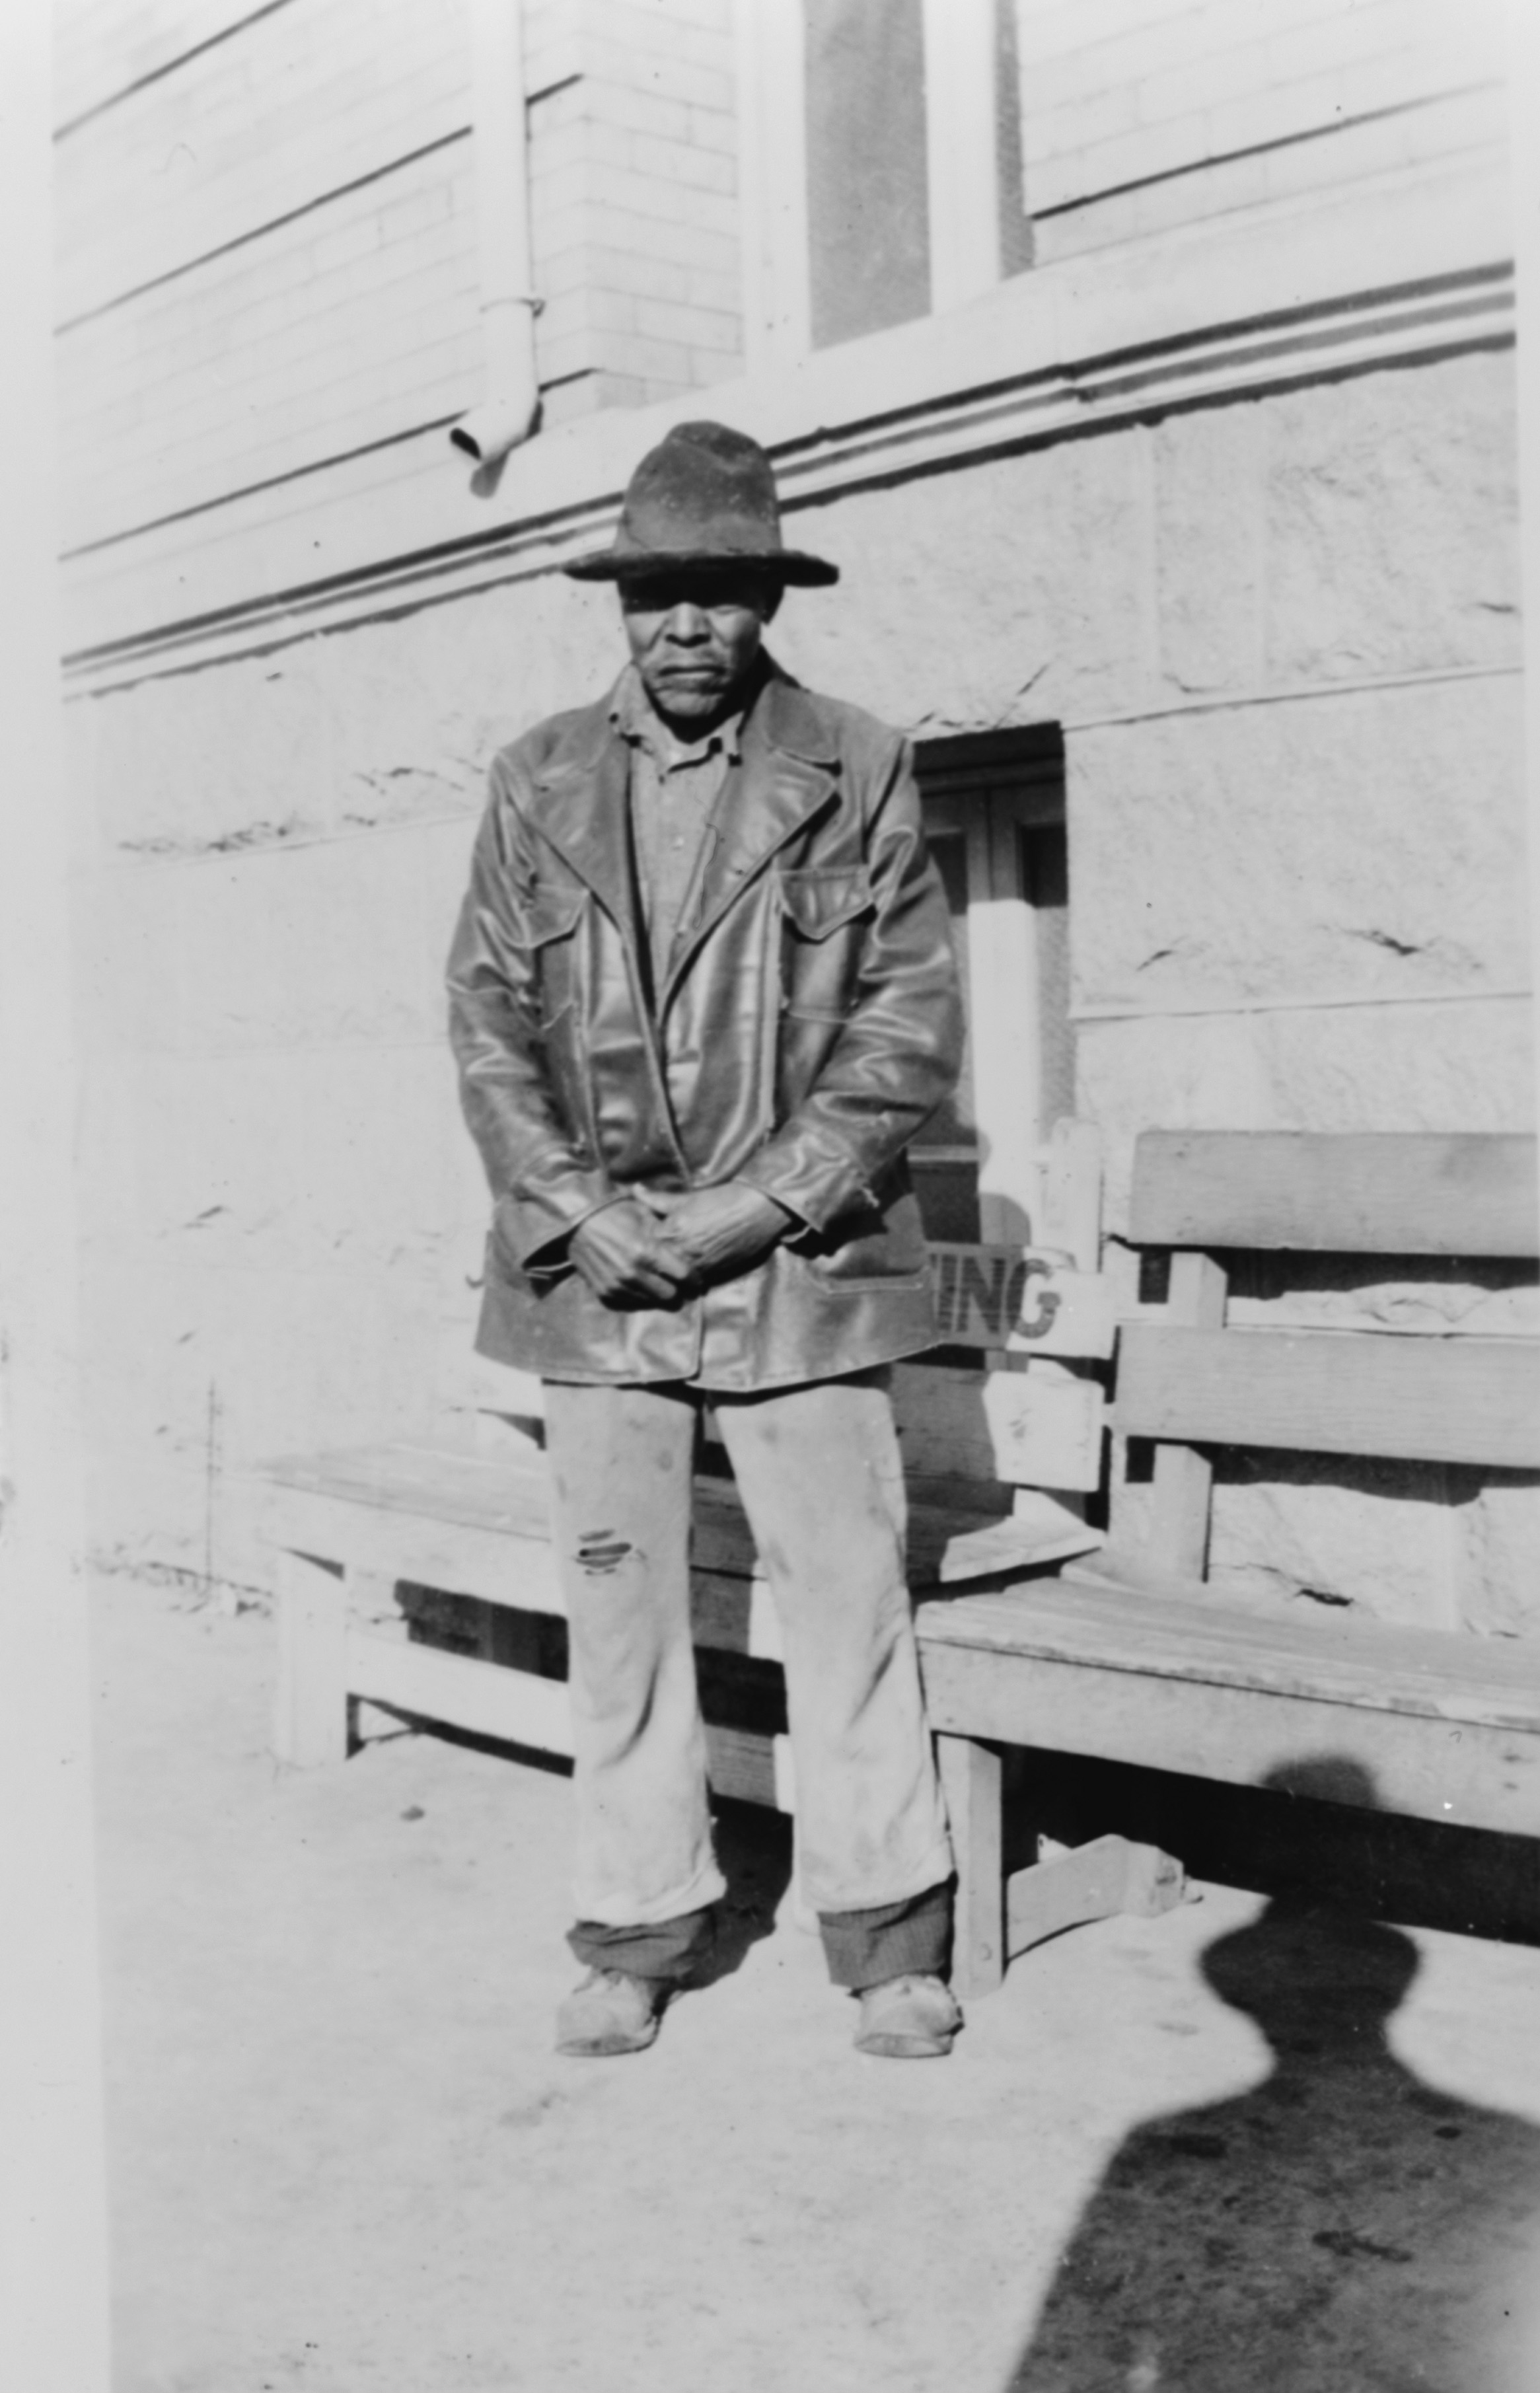
\includegraphics[width=90mm]{./imgs/willadams_recorte.jpg} \label{img14}
\caption{Will Adams}
%\end{minipage}
\end{figure}

\subsection{John White, narrativas do Oklahoma, página 325}
\label{ref284}

``Às vezes, os brancos passavam uma noite na senzala. Não na fazenda dos
Davenport, mas em outras nas redondezas. Os escravos conversavam entre
si sobre isso. Depois de um tempo nascia um bebê novo. Mulatinho. Quando
a criança ficava grande o suficiente para trabalhar um pouquinho, o
senhor vendia ela (ou ele). Não fazia diferença que era sangue do seu
sangue, não se o preço fosse bom!''.

\subsection{Will Adams, narrativas do Texas, Parte I, página 1} \label{ref03}

``Meus pais sempre pertenceram aos Cavins e usaram o seu nome até após a
emancipação. (\ldots{}) Os Cavins sempre gostaram muito dos seus negros,
e Vovó Maria dizia: `Mas é claro! Era o dinheiro deles'".

\subsection{Jacob Manson, narrativas da Carolina do Norte, Parte~\versal{II},~páginas~97--98}
\label{ref181}

``O senhor não tinha filhos com mulher branca. Ele tinha suas namoradas
entre as escravas. Não sou homem de contar mentiras. Eu conto a verdade
e essa é a verdade. Naquele tempo era difícil encontrar um senhor que
não tivesse uma mulher sua entre os escravos. Era uma coisa geral entre
os donos de escravos.

Uma das escravas na fazenda vizinha da nossa foi até a sua senhora e
contou que o senhor estava forçando ela a deixá"-lo ter relações com ela,
e a senhora respondeu: `Ora, pois sim, você pertence a ele'. Outro
senhor, chamado Jimmie Shaw, tinha uma escrava bonitinha, quase branca,
que era sua teúda. A mulher dele pegou os dois na cama na choupana dela.
A mulher disse alguma coisa e ele xingou ela de volta. Ela disse que
tinha pego ele no ato. Ela voltou para a casa grande e pegou uma arma.
Quando o senhor chegou em casa, ela disse que ele devia deixar em paz as
escravas que pertenciam a ela. Ele xingou de novo e mandou que ela
cuidasse do que era da sua conta e ele cuidaria do que era da sua. A
briga ficou feia e então o senhor Shaw foi na direção dela. Ela puxou a
arma e mandou ver. Matou ele na sala mesmo. Eles tinham três filhos,
dois meninos e uma filha casada. A Sra. Shaw pegou seus dois filhos e
foi embora. A filha casada e o marido assumiram a fazenda. A senhora e
os filhos nunca voltaram, que eu saiba.

Muitos dos senhores de escravos tinham alguns escravos fortes e sadios
para atender as escravas. Em geral, eles davam quatro mulheres para um
homem e ai desse homem que tivesse qualquer coisa com as outras
mulheres, e ai dessas mulheres se tivessem alguma coisa com os outros
homens. Quem cuidava das crianças eram as escravas velhas que não
conseguiam trabalhar no eito enquanto as mães dos bebês trabalhavam. As
mulheres aravam e faziam os outros trabalhos, iguais aos homens. Livro e
tudo quanto era estudo eram proibidos''.

\subsection{Tia Carrie Mason, narrativas da Geórgia, Parte~\versal{III},~página~113}
\label{ref183}

``Por que o George {[}seu marido{]} é tão branco? Porque seu senhor era
um cavalheiro branco de nome Sr. Jimmie Dunn. A mãe dela era uma mulher
de cor chamada Frances Mason e o pai era o seu senhor. Sim, senhora,
estou vendo a sua surpresa, mas isso acontecia bastante naqueles tempos.
Ouvi falar de um branco que dizia para os seus filhos, `vão lá na
senzala e me arranjem mais escravos'".

\paragraph{Comentário}\quad
{\small
Outra consequência da ubiquidade do racismo branco e da exploração
da escravidão foi que os escravizados desenvolveram uma consciência
fundamental de si mesmos como membros de um grupo racial. Eles se
consideravam separados e opostos aos brancos e estavam cientes das
diferenças culturais entre as raças. Entre os brancos, comportamentos
alicerçados em solidariedade racial serviam para manter o controle sobre
os escravizados e mantê"-los sob vigilância. Para um cativo nos Estados
Unidos, era quase impossível encontrar uma pessoa branca disposta a
questionar o sistema escravista, e por todos motivos os brancos,
enquanto grupo, nunca seriam dignos de confiança.

Infelizmente, a discriminação brutal continuou a ser realidade
após a emancipação. Durante o período da
Reconstrução, após a Guerra Civil, os ex"-escravos homens conquistaram o
direito ao voto. Até o final do século \versal{XIX}, no entanto, as legislações
estaduais roubaram os direitos ao voto de quase todos os afro"-americanos
do Sul, e o sistema de segregação traçou limites claros entre os
direitos e privilégios usufruídos pelos brancos e a condição subordinada
imposta aos negros. Quando os entrevistados refletiam sobre suas vidas na
escravidão e em liberdade, ao mesmo tempo que se alegravam com o fato de
a escravidão ter se encerrado, muitos ainda tinham sentimentos
conflitantes sobre o que haviam ganhado no processo.
}

\subsection{Susan Hamilton, narrativas da Carolina do Sul, Parte~\versal{II},~página~235}
\label{ref120}

``A raça branca é muito desavergonhada. Eles vêm aqui e expulsam os
índios da própria terra, mas não conseguem fazer eles de escravos porque
os índios não deixam. Eles sobem nas árvores e atiram nos brancos com
flecha envenenada. Os brancos não conseguem fazer eles de escravos,
então vão até a África e trazem os seus irmãos negros e as suas irmãs
negras. (\ldots{})

O tempo todo, noite e dia, se ouvia os homens e as mulheres berrando até
ficarem sem voz quando mãe, pai, irmã ou irmão eram levados e vendidos,
sem aviso nenhum. Às vezes, uma mãe que só tinha um filho era separada
dele para sempre. Vivia morrendo gente de coração partido''.

\subsection{Barbara Haywood, narrativas da Carolina do Norte, Parte~\versal{II},~páginas~386--87}
\label{ref132}

``Você pergunta se os nossos brancos eram bons para a gente, eu digo que
nenhum dos brancos era bom para nenhum dos negros. A gente fiava à noite
e trabalhava duro. Não faltava comida, mas a gente apanhava também''.

\subsection{Virginia Sims, narrativas do Arkansas, Parte~\versal{VI},~páginas~164--65}
\label{ref241}

{[}Ela acredita que era uma jovem adolescente quando a guerra
começou.{]}

``Vi quando estavam se alistando. Eles disseram que iam dar uma sova nos
yankees e iam estar de volta para o desjejum amanhã.

O senhor Ben estava indo e a senhora Susan disse: `Virginia, se você
acha que ele não vai voltar, devia dar um beijo de adeus'. E eu disse:
`Não vou beijar branco nenhum'".

\subsection{Katie Sutton, narrativas do Indiana, página 193}
\label{ref261}

\textls[-10]{``Os brancos são naturalmente diferentes dos negros. Somos diferentes em
cor, na fala e na religião e nas crenças. Somos diferentes em tudo, não
se pode esperar que vamos pensar ou viver igual. (\ldots{}) A velha
senhora e o senhorzinho diziam para as criancinhas escravas que a
cegonha trazia os bebês brancos para as suas mães, mas que os
escravinhos nasciam todos de ovo de urubu, e a gente acreditava que isso
era verdade''.}

\subsection{Minnie Fulkes, narrativas da Virgínia, páginas 11--12} \label{ref95}

``Meu Deus do Céu, eu odeio os brancos e o dilúvio vai afogar mais
deles. (\ldots{}) Deus vai castigar os senhores maus. E se não for eles
a sofrer, o sofrimento vai cair sobre os seus filhos''.

\subsection{Addie Vinson, narrativas da Geórgia, Parte~\versal{IV},~páginas~113--14}
\label{ref270}

``Se aquela gente do Norte não tivesse nos trazido para cá, é certo que
nenhum de nós ia estar aqui para começar. Daí eles foram embora e
disseram que o Sul era ruim para os negros e nos deixaram livres, mas
não vejo diferença nenhuma. O Norte nos deixou por conta depois da
guerra e alguns dos negros velhos ainda estão brabos porque estão livres
e não têm mais senhor para dar nem comida e nem roupa boa e quentinha''.

\subsection{Elijah Green, narrativas da Carolina do Sul, Parte~\versal{II},~página~196}
\label{ref111}


``Foi só após o corpo de John C. Calhoun {[}o político mais famoso e o
defensor mais ferrenho e inflexível da escravidão antes da Guerra
Civil{]} ser levado pela Rua Foundry que o nome foi alterado em sua
homenagem. Ele está enterrado no pátio da Igreja de São Felipe {[}em
Charleston, Carolina do Sul{]}, do outro lado da rua, embaixo de um
loureiro. Quatro homens e eu cavamos a sua cova e limpamos o terreno
onde colocaram o monumento dele. Quem fez o monumento dele foi Pat
Wellington, um pedreiro de Charleston. Nunca gostei de Calhoun, porque
ele odiava os negros; nunca um homem foi tão odiado quanto ele por um
grupo de pessoas''.

{[}Quando os brancos realizavam casamentos{]} ``apenas escravos
especiais eram escolhidos para o casamento. Sempre perguntavam aos
escravos o que eles achavam de quem estava entrando na família. Eu não
gostava, porque tinha que mentir e dizer coisas simpáticas sobre a
pessoa e odiar a pessoa ao mesmo tempo''.

\subsection{Octavia George, narrativas do Oklahoma, página 113} \label{ref105}

``Não havia cadeia, o homem branco era a cadeia dos escravos. (\ldots{})
Vi eles venderem escravos. Os brancos os leiloavam como se faz com gado
ou cavalos hoje em dia. Os escravos bonitos e sadios valiam mais do que
aqueles que não eram tão bons. Vi homens vendidos e separados das
esposas e pensei que aquilo era um crime. Sabia que Deus resolveria as
coisas um dia''.

\subsection{Willis Winn, narrativas do Texas, Parte~\versal{IV},~página~204}
\label{ref304}

``Eles estavam sempre vendendo escravos, colocando a leilão e vendendo,
dependendo de quanto trabalho conseguiam fazer em um dia e a força que
tinham. Vi muitos deles acorrentados, como se fossem vacas e mulas. Se
um dono tinha mais do que precisava, ele pegava a estrada com eles e
vendia para as fazendas vizinhas. Nenhum nunca fugiu. Não tinham para
onde. Vi muitos e muitos tentarem. Se os patrulheiros não pegavam, algum
branco prendia você e chamava o senhor. Eles tinham um acordo de ficar
de olhos abertos para os negros fujões. Quando o senhor o levava de
volta para casa e terminava o serviço, agora você ficava em casa''.
%{[}ESTE PARÁGRAFO APARECEU NO CAPÍTULO 3 QUASE EXATAMENTE IGUAL.{]}%MANTER?

\subsection{Mark C. Trotter, narrativas do Arkansas, Parte~\versal{VI},~página~353}
\label{ref264}

``Meus donos eram a Sra. Betty e o Sr. Luke Trotter. Eu nasci no Condado
de Tunica, Mississippi. Lavrei a terra toda a vida. Eu gostava. Uma
coisa que se dizia da escravidão era que não tinha como escapar. Eles
tinham cães, e quem fugia não tinha para onde ir, não tinha o que comer.
Viajar era difícil na mata fechada. Um dono avisava o outro sobre o
fujão. Eles levavam ele de volta ou mandavam chamar para buscar o fujão.
Alguns tentavam ficar no mato. Dizem que nunca tentavam escapar. Eu só
nasci depois da liberdade. Dizem que tinham pena quando alguém apanhava,
mas não tinham o que fazer. Eles simpatizavam com a sua cor''.

\subsection{Anne Bell, narrativas da Carolina do Sul, Parte~I,~página~53--54} \label{ref22}

``Se eu acredito em religião? O que mais tem para os negros? Eu lhe
pergunto, se não existe Céu, o que é que os negros têm de esperança?
Aqui embaixo eles não vão a lugar nenhum. A única alegria que têm aqui é
servir e amar. A gente tem isso na religião, mas em todo o resto o negro
tem um limite''.

\subsection{Alice Douglass, narrativas do Oklahoma, página 74} \label{ref74}

``Hoje os brancos não querem que você encoste neles, mas eu dormi com
crianças brancas até fazer 19 anos. Dá para cozinhar para eles e botar
as mãos na comida e eles não dizem nada, mas ai de quem encosta neles!''.

\subsection{William McWhorter, narrativas da Geórgia, Parte~\versal{III},~páginas~102--03}
\label{ref191}

``Pois a senhora sabe que todos os negros preferem ser livres, e nisso
eu não sou diferente de ninguém. Sim, senhora, eu fico muito contente
que o Sr. Abraham Lincoln e Jeff Davis brigaram até nos libertar. Aquele
Jeff Davis devia ter vergonha de si mesmo, querendo manter os negros em
cativeiro. Mas dizem que ele era um homem muito bom, e Dona Miss Millie
Rutherford disse umas coisas muito bonitas sobre ele naquele livro que a
Sarah leu para mim, mas você não vai esperar que os negros vão achar que
ele era assim tão boa gente.

Fico muito feliz que o Bom Deus decidiu nos libertar do pecado e da
escravidão. Se não tivesse, eu teria morrido muito tempo atrás''.

\subsection{Tia Ferebe Rogers, narrativas da Geórgia, Parte~\versal{III},~páginas~212--13}
\label{ref228}

``Tia Ferebe, hoje em dia é melhor, ou você acha que os tempos da
escravidão eram mais felizes? `Ora, você me pediu a verdade, não foi? E
eu vou contar a verdade. Eu não minto. Sim, senhora, esses tempos de
hoje são melhores para mim. Acho que é melhor trabalhar para si e ficar
com o que faz do que ter que trabalhar para os outros e não tirar nada
disso. Os dias da escravidão eram duros, muito duros. Meu senhor era bom
para nós (quer dizer, ele não nos batia muito, e sempre nos deu bastante
comida), mas alguns escravos sofriam um horror. Minha tia foi espancada
de um jeito cruel uma vez, e vários outros escravos (\ldots{}) Eu levei
surras, várias delas'".

\subsection{Esposa de Charles Douthit, narrativas\break do Missouri, página 107} \label{ref75}

``Enquanto o entrevistador questionava Charles Douthit, de
Farmington, Missouri, homem negro, nascido em 1865, sua esposa estava
parada na porta, assistindo tudo com os olhos arregalados. Incapaz de se
conter, ela finalmente exclamou o seguinte: `Ora! Para que estão fazendo
todas essas perguntas, afinal? Aposto que eu sei. Querem descobrir como
é que tratavam os escravos de antigamente para saber como tratar os mais
novos quando fizerem eles de escravos. Aposto que vão tentar ter
escravos de novo, e tem gente que quer a escravidão de volta, mas hoje
as pessoas não vão aceitar. Não sei o que o governo quer fazer, mas
teria uma guerra muito terrível se tentassem ter escravos de novo'".

\pagebreak
\thispagestyle{empty}
\movetoevenpage
\thispagestyle{empty}

\begin{absolutelynopagebreak}
\begin{vplace}
\begin{figure}[H]
\begin{adjustwidth}{-1.6cm}{}
  %\centering
  \vspace*{-2cm}
  %\hspace{-0.5cm}
  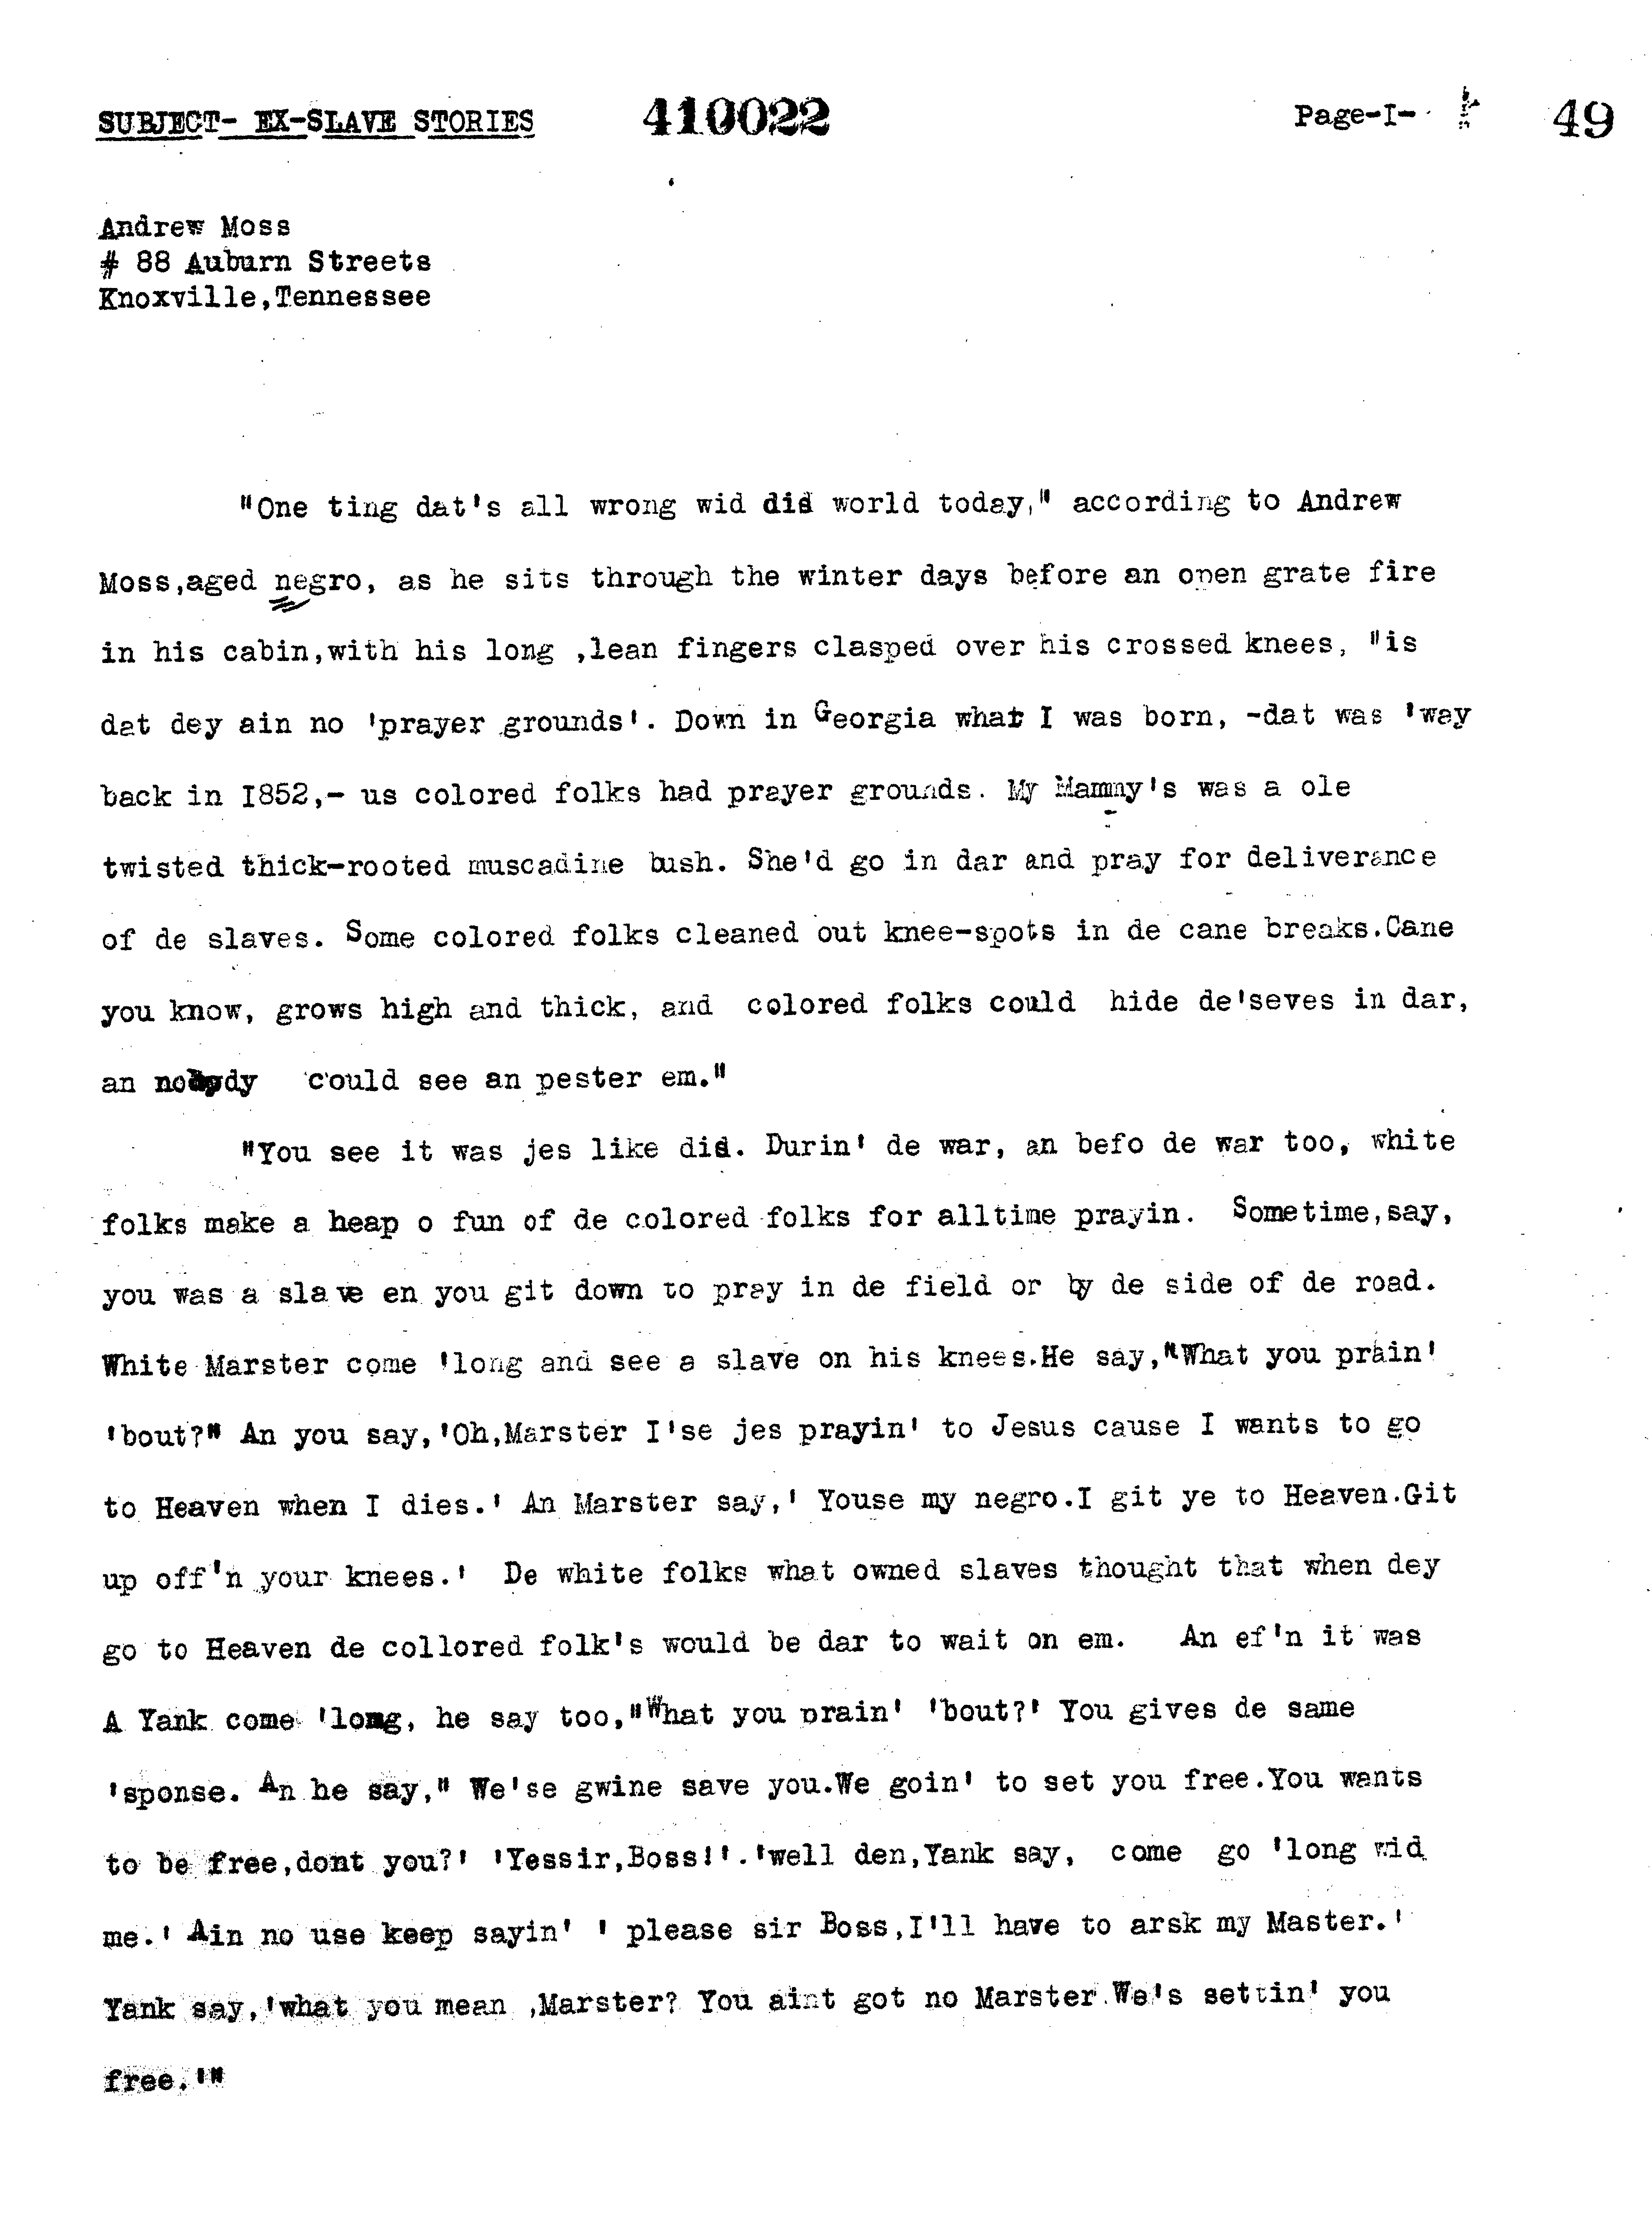
\includegraphics[width=130mm]{./imgs/Cap6.jpg}  
  %\hfill
\end{adjustwidth}
  \caption{Andrew Moss, narrativas do Tennessee, página 49}
\end{figure}
\end{vplace}

\end{absolutelynopagebreak}

\chapter{Cultura negra}
%\addcontentsline{toc}{chapter}{{\large\versal{VI.}} Cultura negra}
%\hedramarkboth{Cultura negra}{}

\subsection{Andrew Moss, narrativas do Tennessee, página 49}
\label{ref202}

```Uma coisa que tem de errado no mundo de hoje', afirma Andrew Moss,
negro idoso, que passa os dias de inverno sentado perante a lareira
aberta em sua choupana, dedos longos e magros entrelaçados sobre os
joelhos cruzados, `é que não existem mais \emph{terrenos de reza}. Lá na
Geórgia, onde eu nasci, isso lá em 1852, nós tínhamos terrenos de reza.
O da minha mamãe era um arbusto de muscadínea velho, com as raízes bem
grossas e torcidas. Ela ia lá para rezar pela salvação dos escravos.
Alguns negros limpavam espaços para se ajoelhar no meio do canavial. A
cana cresce alta e grossa, sabe, e os negros se escondiam lá dentro e
ninguém incomodava eles.

Pois era bem assim, sabe. Durante a guerra, e antes da guerra também, os
brancos faziam muita troça dos negros por tudo o que rezavam. Às vezes,
por exemplo, você era escravo e se ajoelhava no eito para rezar, ou na
beira da estrada. O senhor branco aparecia e via um escravo de joelhos.
`Para que você está rezando?', ele perguntava. `Ah, senhor, só estou
rezando para Jesus porque quero ir para o Céu quando morrer', você
respondia. `Você é meu negro', o senhor respondia. `Eu mando você
para o Céu. Já de pé'. Os brancos que tinham escravos achavam que
quando fossem para o Céu, os negros iam estar lá de serviçais para eles.
E se era um yankee que aparecia, ele também perguntava: `Para que você
está rezando?' Você dava a mesma resposta e ele dizia: `Nós vamos
salvar vocês, vamos libertar vocês'\,'".

\paragraph{Comentário}\quad
{\small
Sem uma cultura independente própria, com elementos essenciais
opostos aos ensinamentos dos brancos, os escravizados teriam tido
dificuldade para resistir às forças corrosivas da escravidão. Mas todas
as fontes concordam que a sua cultura era diferente, e as perguntas dos
entrevistadores sobre religião, conjuro ou superstições ajudam a trazer
isso à tona. Os costumes e atitudes de vida que vicejavam na comunidade
escrava diferenciavam os seus membros dos proprietários brancos.

As fazendas escravistas nos Estados Unidos quase nunca tinham suas
próprias igrejas, mas a religião era uma parte importante da cultura
negra. As denominações batistas e metodistas eram as mais populares
entre os senhores de escravos, muitos dos quais insistiam que seus
cativos os acompanhassem aos cultos nas igrejas brancas. Neles, os
pastores pregavam uma versão pró"-escravista do Evangelho ou davam
sermões especiais para os escravizados. Rejeitando esse tipo de fé,
eles desenvolveram o seu próprio Cristianismo e passaram a praticar
a religião à própria maneira, quase sempre em segredo. Muitos se retiravam para ``terrenos de reza'' ou ``pérgolas'' no mato, onde podiam orar a Deus.

Tanto no Norte quanto no Sul, os brancos comentavam sobre o que
para eles era a natureza incomum, ou inusitada, dos cultos dos escravizados,
que envolviam ``gritos'' de êxtase e podiam incluir rodas de dança
intensas. Os brancos também observavam que as vestimentas escravas
eram distintivas, apesar do fato de os proprietários normalmente
fornecerem uma parca quantidade de roupas aos seus escravizados. Em alguns
casos, as mulheres negras cobriam suas cabeças com lenços coloridos, e
muitas vezes faziam tranças nos cabelos, amarrando"-os com pedaços de
fio. Alguns cativos também praticavam conjuro para lançar feitiços
contra outras pessoas, tanto brancas quanto negras. O conjuro vinha de
influências africanas e caribenhas, e provavelmente também dos brancos
no interior e da cultura nativa americana, e os escravizados tinham uma
série de crenças sobre raízes medicinais e as propriedades terapêuticas
de plantas e ervas.

Entretanto, o mais importante para a ideia que os escravizados faziam
de si mesmos enquanto grupo que poderia sobreviver e superar a
escravidão um dia era a sua fé. O seu Cristianismo era uma
religião de justiça e igualdade, com um Salvador que se importava com
eles, sentia o seu sofrimento e os recompensaria no final. Assim, este
capítulo começa principalmente com descrições dos entrevistados sobre a
sua religião e práticas religiosas.
}

\subsection{Mary Gladdy, narrativas da Geórgia, Parte~\versal{II},~páginas~17,~24,~26--27}
\label{ref106}

``O pai do meu pai era um negro africano de sangue puro, baixinho e bem
escuro, que mal falava inglês. (\ldots{}) Acho que ele não tinha nem um
metro e meio e mal se entendia o que ele falava''.


\noindent{}\emph{Velho Cântico dos Escravos}\\
\noindent{}{[}Cantado para o entrevistador{]}

\begin{verse}
My sister, I feels `im, my sister I feels `im;\\
All night long I've been feelin `im;\\
Jest befoe day, I feels `im, jest befoe day I feels `im;\\
The sperit, I feels 'im, the sperit I feels `im!\\
My brother, I feels `im, my brother I feels `im;\\
All night long I've been feelin `im,\\
Jest befoe day, I feels `im, jest befoe day, I feels `im;\\
The sperit, I feels 'im!\footnotemark
\end{verse}

\footnotetext{Tradução: ``Irmã, eu o senti,
irmã, eu o senti;/ A noite inteira eu o senti;/ Logo antes
do dia nascer, eu o senti, logo antes do dia nascer, eu o senti;/ O espírito, eu o
senti, o espírito, eu o senti!/ Irmão, eu o senti,
irmão, eu o senti;/ A noite inteira eu o senti,/ Logo antes
do dia nascer, eu o senti, logo antes do dia nascer, eu o senti;/ O espírito, eu o senti!''}

``De acordo com Mary Gladdy, ex"-escrava, 806 ½ --- Sexta Avenida,
Columbus, Geórgia, era costume entre os escravos durante o período da
Guerra Civil se reunir em segredo nas suas choupanas duas ou três noites
por semana para cultos e orações. Uma grande panela de ferro sempre era
colocada contra a porta de entrada, de lado, para não deixar o som das
suas vozes `escapar' ou ser escutado do lado de fora. {[}Provavelmente
mais importante era o fato de os casebres dos escravizados normalmente
ficarem localizados a uma certa distância, 50 metros ou mais, da casa do
senhor.{]} Depois, os escravos cantavam, rezavam e relatavam suas
experiências a noite inteira. O grande desejo que ardia em suas almas
era pela liberdade. Não é que eles amavam os yankees ou odiavam seus
senhores, eles meramente ansiavam por ser livres e odiavam a instituição
da escravidão.

Praticamente sempre, todos os negros que participavam dessas reuniões
sentiam o espírito do Senhor `tocá"-lo (ou tocá"-la) logo antes do dia
nascer'. Nesse momento, todos se erguiam, apertavam as mãos e começavam
a entoar o cântico citado acima. Era o sinal para o encerramento e, após
entoar por 15 ou 20 minutos, todos apertavam as mãos mais uma vez e iam
para casa, confiantes em seus corações que a liberdade era o seu
destino''.

{[}Mary Gladdy também cantou:{]}

\noindent{}``\emph{Keek the fire burning while your soul's fired up}.''\\
\noindent{}{[}Mantenho o fogo aceso enquanto a sua alma está em chamas.{]}

\begin{verse}
Fire, fire, O, keep the fire burning while your soul's fired up,\\
O, keep the fire burning while your soul's fired up;\\
Never mind what satan says while your soul's fired up,\\
You ain't going to learn how to watch and pray,\\
Less you keep the fire burning while your soul's fired up.\\
Old Satan is a liar and a cunjorer, too;\\
If you don't mind, he'll cunjor you;\\
Keep the fire burning while your soul's fired up.\\ 
Never mind what satan says while your soul's fired up.\footnotemark
\end{verse}
\footnotetext{Tradução: ``Fogo, fogo, ah, mantenha o fogo aceso enquanto a sua alma está em
chamas,/ Ah, mantenha o
fogo aceso enquanto a sua alma está em chamas;/ Não escute o
que Satã diz enquanto a sua alma está em chamas,/ Você não vai aprender
a velar e a rezar,/ A menos
que mantenha o fogo aceso enquanto a sua alma está em chamas./ O velho Satã é mentiroso e
feiticeiro também;/ Se não tomar cuidado, ele
enfeitiça você;/ Mantenha o fogo
aceso enquanto a sua alma está em chamas./ Não escute o
que Satã diz enquanto a sua alma está em chamas.''}

\subsection{George Womble, narrativas da Geórgia, Parte~\versal{IV},~página~189}
\label{ref309}

``Algumas noites, eles iam para o mato e realizavam seu próprio culto.
Em um determinado local, todos se ajoelhavam e viravam os rostos para o
chão, então começavam a gemer e a rezar. O Sr. Womble diz que se
ajuntando nesse círculo e virando suas vozes para o solo, o som não se
propagava muito''.

\subsection{Thomas Anderson Carlisle, narrativas da Carolina~do~Sul,~Parte~II,~página~62}

``As meninas vinham em vestidos engomados para o culto ao ar livre. Elas
baixavam o cabelo e desfaziam as tranças para o culto. Naqueles tempos,
todas as negras usavam o cabelo em tranças, exceto quando iam à igreja
ou a um casamento. Nos cultos, as mulheres tiravam os panos da cabeça,
menos as mães. Nessas ocasiões, as mães usavam panos de linho
recém"-lavados na cabeça''.

\subsection{Ann Matthews, narrativas do Tennessee, página 45}
\label{ref184}

``Durante a escravidão, os brancos não queriam que os negros cantassem e
rezassem, mas eles viravam uma panela de boca para baixo e se reuniam na
panela de noite para cantar e rezar e os brancos não escutavam.

Se um escravo morria, os brancos não deixavam ninguém ficar com o corpo,
exceto os negros da fazenda, mas os outros negros se escapuliam depois
que escurecia, ficavam com o corpo e depois voltavam escondidos para as
suas fazendas antes do dia nascer''.

\subsection{Lucy Brown, narrativas da Carolina do Norte, Parte~\versal{II},~página~193} \label{ref38}

``O senhor era bom para a gente, do seu jeito, mas ele não deixava
ninguém brincar, então quando a gente fazia uma reunião, tinha que ser
em segredo. A gente virava uma tina no lado de fora da porta para
segurar a bagunça, então o senhor nunca sabia de nada''.

\subsection{Silvia King, narrativas do Texas, Parte \versal{II}, página 294}
\label{ref166}

``Os negros se mandavam para as baixadas para gritar e cantar e rezar.
Eles faziam uma roda de dança. No começo meio que só arrastam o pé, daí
vai ficando mais rápido e mais rápido, eles se esquentam e começam a
gemer e a gritar, a bater palmas e a dançar. Uns ficam exaustos e caem
para fora, então a roda se aperta mais um pouco. Às vezes, eles cantam e
gritam madrugada adentro, mas quando raia o dia o negro tem que estar na
choupana. O velho senhor tem que dizer quais são as tarefas do dia''.

\subsection{Essex Henry, narrativas da Carolina do Norte, Parte~I,~página~396}
\label{ref137}

``Pois sabe que a religião era coisa proibida naquela fazenda. A velha
Betsy Holmes foi açoitada várias e várias vezes por falar em religião e
por cantar hinos. A gente ainda fazia uns cultos de vez em quando nas
choupanas, mas antes virava um panelão na frente da porta para segurar o
barulho''.

\subsection{Elisha Doc Garey, narrativas da Geórgia, Parte~\versal{II},~página~5} \label{ref100}

``Alguns poucos escravos sabiam ler e escrever, e os que sabiam ler
quase sempre eram chamados pelos outros para pregarem. Charlie McCollie
foi o primeiro pastor negro que vi. Os brancos permitiam que os escravos
usassem pérgolas de igrejas nas fazendas, e os negrinhos e as negrinhas
faziam uns belos namoros naquelas pérgolas. Era o único lugar onde dava
para ver as meninas que você mais gostava. O culto costumava iniciar com
uma música, \emph{Come Ye Dat Loves De Lawd} {[}Venha, vós que amastes o
Senhor{]}. As igrejas não tinham pia para batizar ninguém, então
levavam todo mundo para o riacho. Primeiro um diácono entrava e media a
água com uma vara para encontrar um lugar seguro e correto, daí estava
tudo pronto para o pastor e os candidatos. Todo mundo ficava de pé na
margem do riacho, cantando juntos. Algumas das músicas: \emph{Lead Me to de
Water to be Baptized} {[}Leve"-me à água para ser batizado{]}, \emph{Oh, How
I Love Jesus} {[}Ah, como amo Jesus{]} e \emph{Oh, Happy Day dat Fixed my
Choice} {[}Oh, dia feliz em que fiz minha escolha{]}''.

\subsection{Tom Hawkins, narrativas da Geórgia, Parte~\versal{II},~página~131}
\label{ref128}

``Nenhum de nós sabia ler a Bíblia e nenhum dos negros da nossa fazenda
se converteu, então a gente nunca teve batizado nenhum. O pastor pregava
primeiro para os brancos e depois, quando pregava para os negros, tudo
que ele dizia era: `Roubar é pecado, não roubem as galinhas e os porcos
do senhor e da senhora' e coisas assim. Como é que alguém ia se
converter com uma pregação dessas? Além do mais, nunca adiantou nada
escutar essas pregações, porque os roubos seguiram acontecendo todas as
noites''.

\subsection{Minnie Johnson Stewart, narrativas do Arkansas, Parte~\versal{VI},~página~236}
\label{ref253} 

``Ela {[}sua mãe{]} nos contou como os escravos costumavam tentar rezar.
Eles tinham tanto medo de o feitor vê"-los que, no início da manhã, indo
para o eito trabalhar quando o sol nascia, se ajoelhavam com uma perna
para rezar. Tinham tanto medo de serem pegos pelo feitor que ficavam
cuidando ele com um olho e olhando para Deus com o outro. Mas o Senhor
entendia''.

\subsection{Amanda McCray, narrativas da Flórida, página 215}
\label{ref185}

``Havia um terreno de reza onde a `grama nunca conseguia crescer, pois
os joelhos angustiados estavam sempre esmagando a terra'".

\subsection{Charlie Aarons, narrativas do Alabama, páginas 2--3} \label{ref02}

``Sábado à noite, eles podiam cantar e dançar nas senzalas e realizar
cultos, e em alguns domingos podiam prender as mulas a uma grande
carroça e irem todos juntos à igreja dos brancos; e lá também se
realizava cultos ao ar livre, do qual participavam escravos vindos de
todas as fazendas vizinhas, alguns chegando nas mesmas grandes carroças,
com até quatro mulas por carroça. Eles se divertiam bastante no caminho,
cantando e chamando uns aos outros e fazendo amizades''.

\subsection{Wes Brady, narrativas do Texas, Parte I, página 135} \label{ref32}

``Íamos à igreja na fazenda, mas você devia escutar só aquelas
pregações. Obedeçam o senhor e a senhora, não roubem galinhas e ovos e
carnes, mas nem uma palavra sobre ter uma alma a salvar''.

\begin{figure}[]
%\begin{minipage}{0,4\textwidth}
\centering
 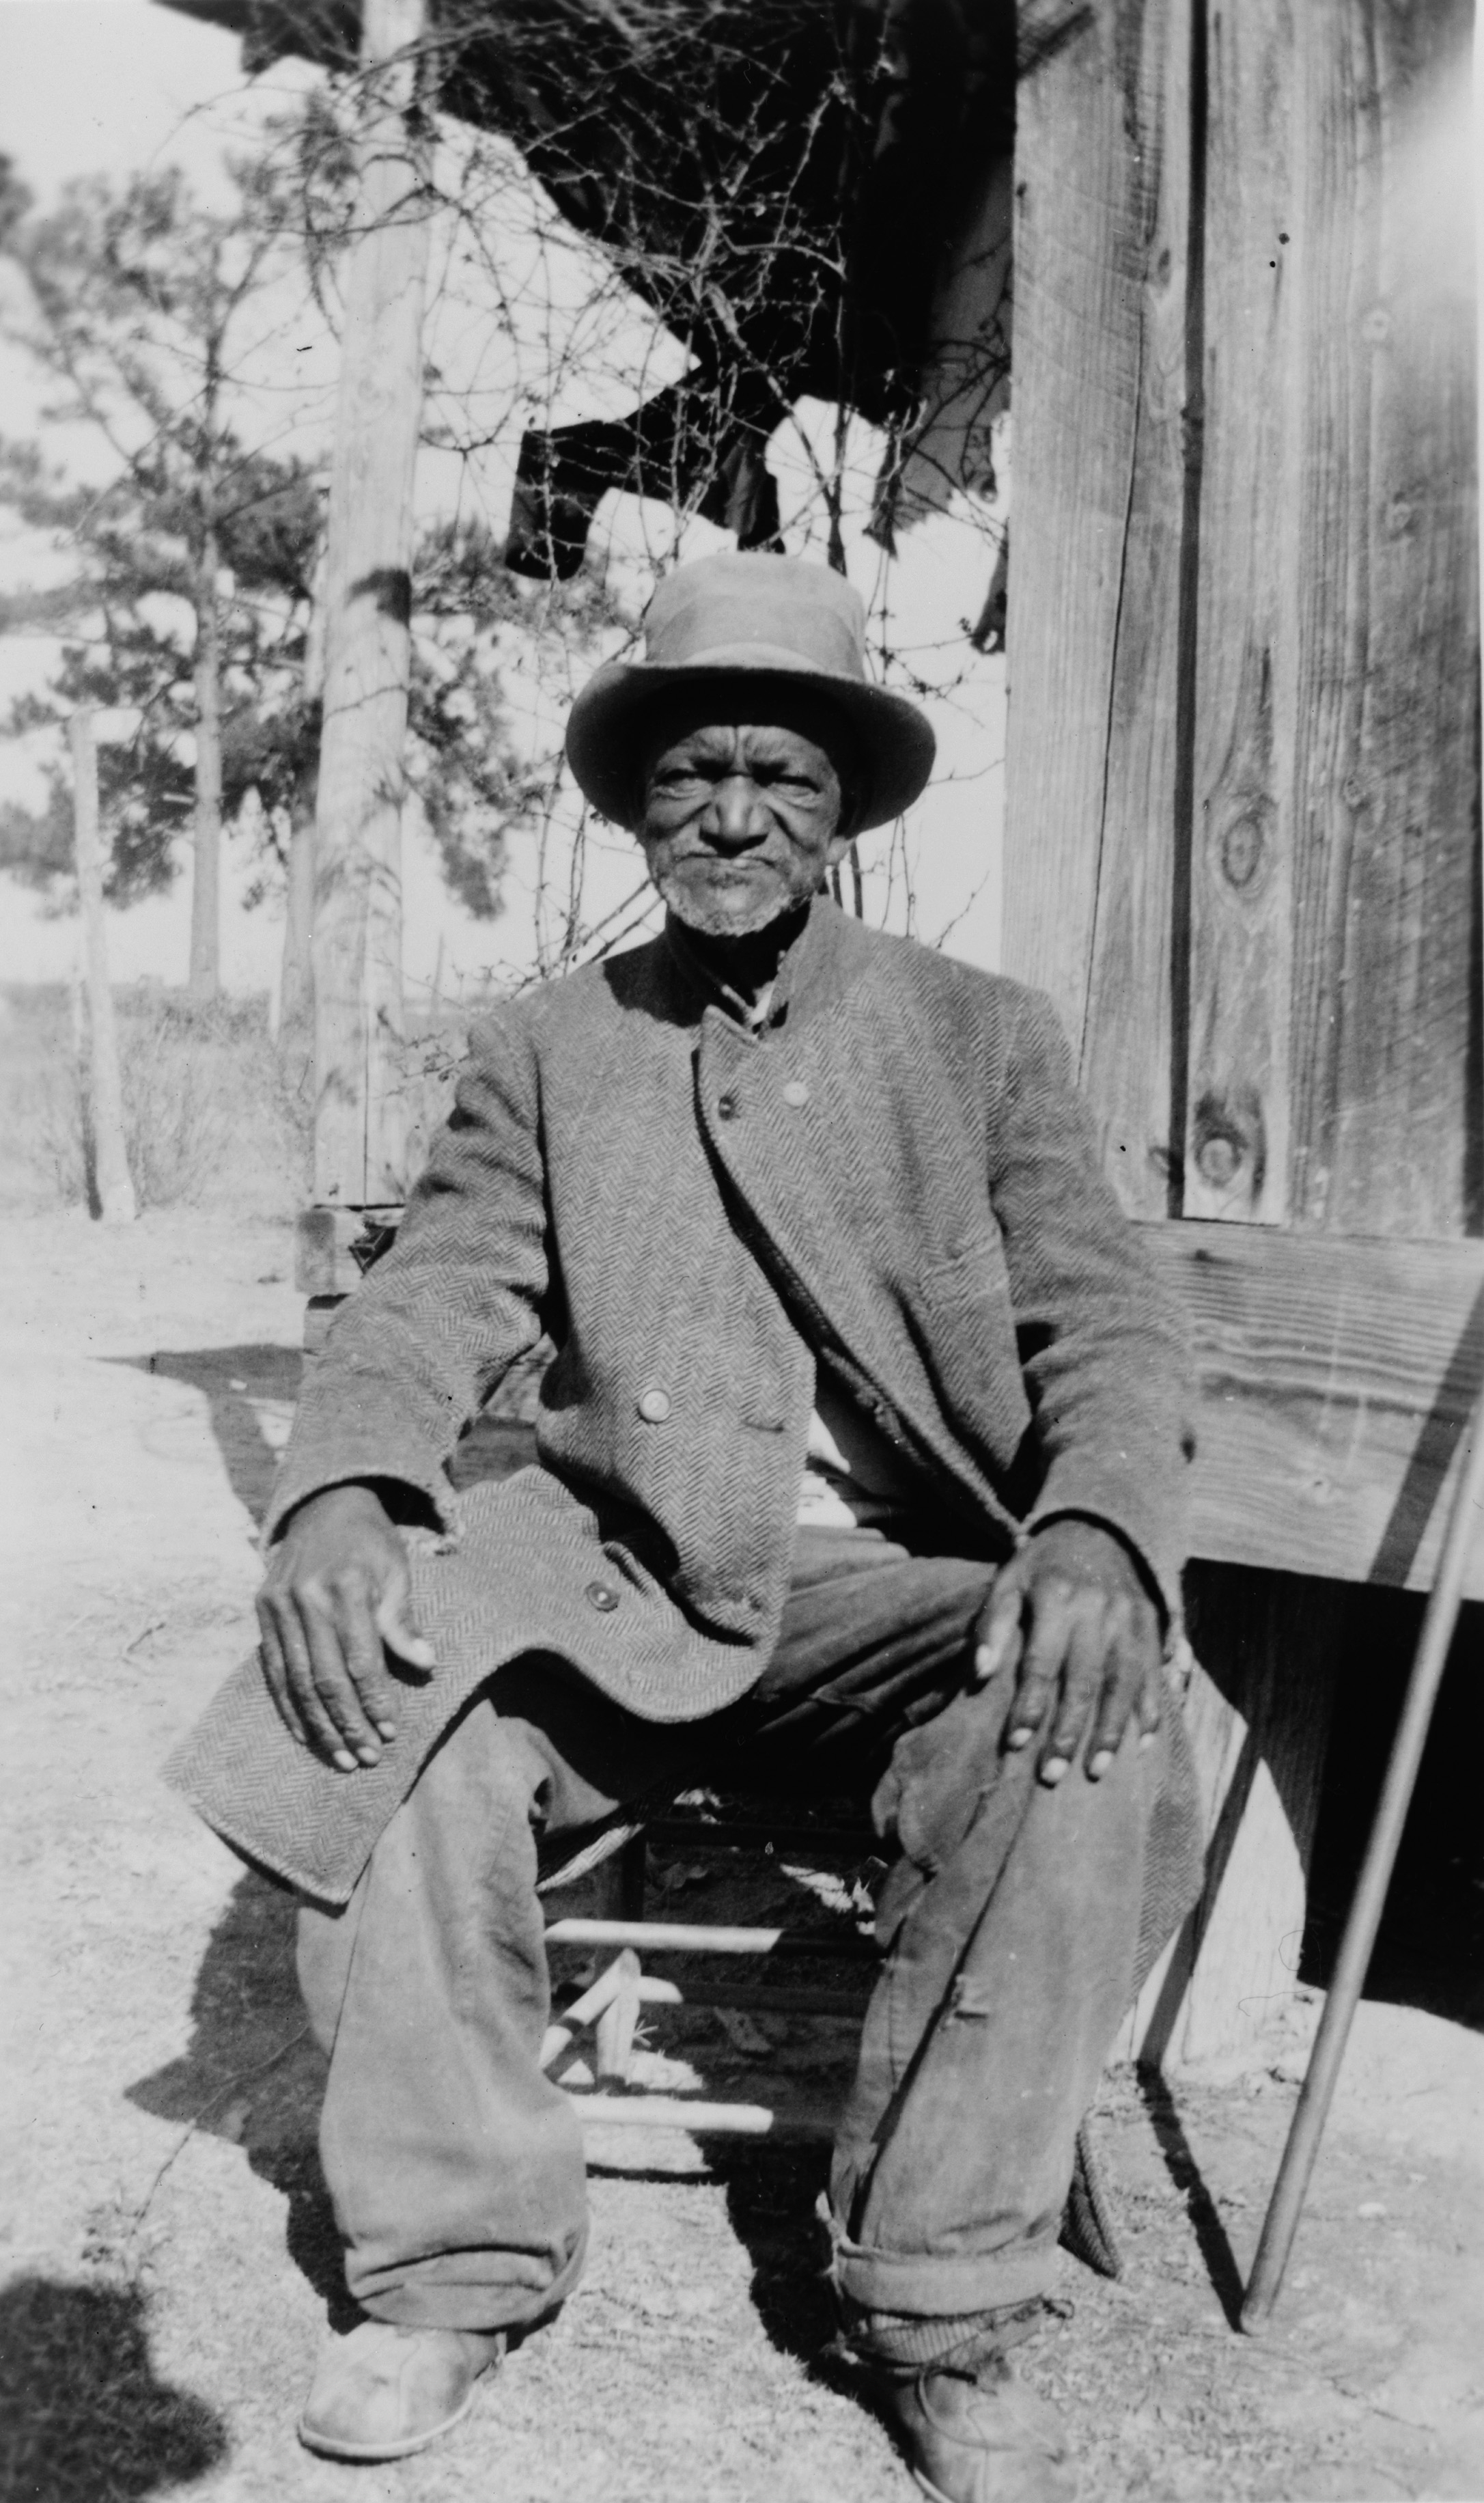
\includegraphics[width=90mm]{./imgs/wesbrady_recorte.jpg} \label{img15}
\caption{Wes Brady}
%\end{minipage}
\end{figure}

\subsection{Margaret Hughes, narrativas da Carolina do Sul, Parte~\versal{II},~página~329}
\label{ref154}

``Sim, senhora, sobre esses casamentos que me perguntou; bem, a gente
fazia uma festa quando qualquer um dos escravos se casava. O senhor e a
senhora deixava eles casarem na casa grande e depois se fazia um bailão
numa das senzalas. Os brancos davam tudo quanto é coisa de comer e os
negros davam a música para dançar. O irmão da minha mãe era um dos
melhores rabequeiros de todos, ele ensinava os outros negros a tocar.

As vezes que a gente mais se divertia era durante o verão, indo aos
cultos ao ar livre. Tinha bons homens para pregar o culto, depois todas
nós se juntávamos e montávamos um belo almoço de piquenique, trazido de
casa em cestas, e fazíamos uma festa. Alguns comiam tanto que chegavam a
passar mal. Não se tinha tanta doença naquela época, não como se tem
hoje. A gente usava alho e assafétida em volta do pescoço para espantar
as doenças, e nunca teve muito. Fomos vacinados para ninguém pegar
varíola''.

\subsection{Emoline Glasgow, narrativas da Carolina do Sul, Parte~\versal{II},~página~135}
\label{ref107}

``Uma vez, o senhor Gilliam levou um dos seus escravos para a igreja em
Tranquil e disse que ele não podia gritar naquele dia, disse que daria
para ele um par de botas novas se não gritasse. No meio do culto, o
velho negro não se aguentou mais. Ele deu um pulo e berrou: `Com bota ou
sem bota, hoje eu vou gritar'".

\subsection{Anthony Dawson, narrativas do Oklahoma, página 69} \label{ref70}

``O velho senhor era um bom cristão, mas ainda gostava do seu julep. Ele
deixava os negros com as suas rezas e pregações e nos liberava para
viajar 15, 20 quilômetros até um culto ao ar livre e ficar dois ou três
dias, só com a palavra do Tio John. Nossos pastores eram quase todos
brancos, mas quando aparecia um pastor negro, era o Paraíso.

Não tinha mulher de vodu nem conjurador nos nossos 8 hectares, todos nós
conhecíamos a Palavra e o Filho de Deus invisível e não botávamos fé no
conjuro''.

\subsection{Henry Wright, narrativas da Geórgia, Parte \versal{IV}, página 201}
\label{ref320}

``Aos domingos, o Sr. House obrigava todos os seus escravos a irem à
igreja. Todos frequentavam a igreja branca, onde sentavam"-se ao fundo ou
na sacada interior. Após pregar para o público branco, o pastor branco
voltava sua atenção para os escravos. O sermão geralmente se conformava
à seguinte linha: `Obedeçam seus senhores e senhoras e Deus vai
amá"-los'. Às vezes, um pastor negro tinha permissão para pregar do mesmo
púlpito após o pastor branco terminar. Seu sermão seguia uma linha
semelhante, pois era isso que ele havia sido instruído a dizer. Nenhum
dos escravos acreditava nos sermões, mas eles fingiam acreditar''.

\subsection{Anderson Edwards, narrativas do Texas, Parte \versal{II}, página 9} \label{ref80}

``Eu prego o Evangelho e trabalho na fazenda desde o tempo da
escravidão. Entrei para a igreja quase 83 anos atrás, quando era escravo
do Major Gaud, e me batizaram na nascente mais próxima de onde encontrei
o Senhor. Quando comecei a pregar, não sabia ler nem escrever e tinha
que pregar o que o senhor me dizia. Ele me mandava dizer para os negros
que se obedecerem o senhor eles vão para o Céu. Eu sabia que tinha algo
melhor para eles, mas não tinha coragem de contar, exceto às escondidas.
Isso eu fiz bastante. Eu dizia que se seguissem rezando, o Senhor ia
libertá"-los''.

\subsection{Clara C. Young, narrativas do Mississippi, páginas 171--72}
\label{ref322}

``O mais que a gente se divertia era nos cultos. Tinha um quase todos
os domingos, e eles entravam noite adentro. O pastor que eu mais gostava
se chamava Matthew Swing. Era um negro bonito, preto feito a noite, e
ele sabia ler com as mãos. Nunca aprendeu a ler nem a escrever de
verdade, mas conhecia bem a Bíblia e esticava a mão para a frente e
fingia que estava lendo. Ele pregava a pregação mais bonita que já se
ouviu. O culto ia do começo da manhã até tarde da noite. Quando ficava
escuro, os homens penduravam uma tina de lavar roupa de cabeça para
baixo na nossa igrejinha do mato, para segurar o barulho e não deixar o
feitor nos escutar cantando e gritando. Eles não se importavam com o
culto de dia, mas achavam que se a gente passasse metade da noite
acordados, ninguém ia trabalhar tanto no outro dia. E era verdade''.

\subsection{Douglas Dorsey, narrativas da Flórida, páginas 97--98} \label{ref71}

``Ocasionalmente, os escravos recebiam a ordem de ir à igreja escutar o
sermão de um pastor branco. Eles se sentavam nos bancos da frente da
igreja dos senhores, enquanto os brancos sentavam"-se ao fundo. O pastor
os advertia que era preciso honrar seus senhores e senhoras e não
guardar nenhum Deus além deles, pois `não temos como ver o outro Deus,
mas vocês veem seus senhores e senhoras'. Após o culto, a esposa do
cocheiro, que sabia ler e escrever um pouco, explicava para eles que
aquilo que o pastor dissera `era tudo mentira'".

\subsection{Minerva Edwards, narrativas do Texas, Parte~\versal{II},~páginas~6--7} \label{ref82}

``Não trabalhávamos no eito aos domingos, mas tinha tanto gado para
cuidar que a gente ficava ocupado. A senhora era religiosa e sempre nos
levava para a igreja quando podia. Quando a gente rezava por conta,
ninguém tinha coragem de deixar os brancos saberem, então se virava uma
tina para o chão para prender as vozes. A gente rezou muito para ser
livres, e o Senhor nos escutou. Não tinha nenhum hinário, mas o Senhor
nos deu nossas canções. Quando a gente cantava elas à noite, era
cochichando, para ninguém nos escutar. Uma delas era assim:

\begin{verse}
My knee bones am aching,\\
My body's rackin' with pain,\\
I 'lieve I'm a chile of God,\\
And this ain't my home,\\
`Cause Heaven's my aim.\footnotemark
\end{verse}

\footnotetext{Tradução: ``Meus ossos do joelho doem,/ Meu corpo é assolado pela dor,/ Acredito que sou filho de Deus,/ E este não é meu lar,/ Pois minha meta é o Paraíso.''}

\begin{figure}[!ht]
%\begin{minipage}{0,4\textwidth}
\centering
 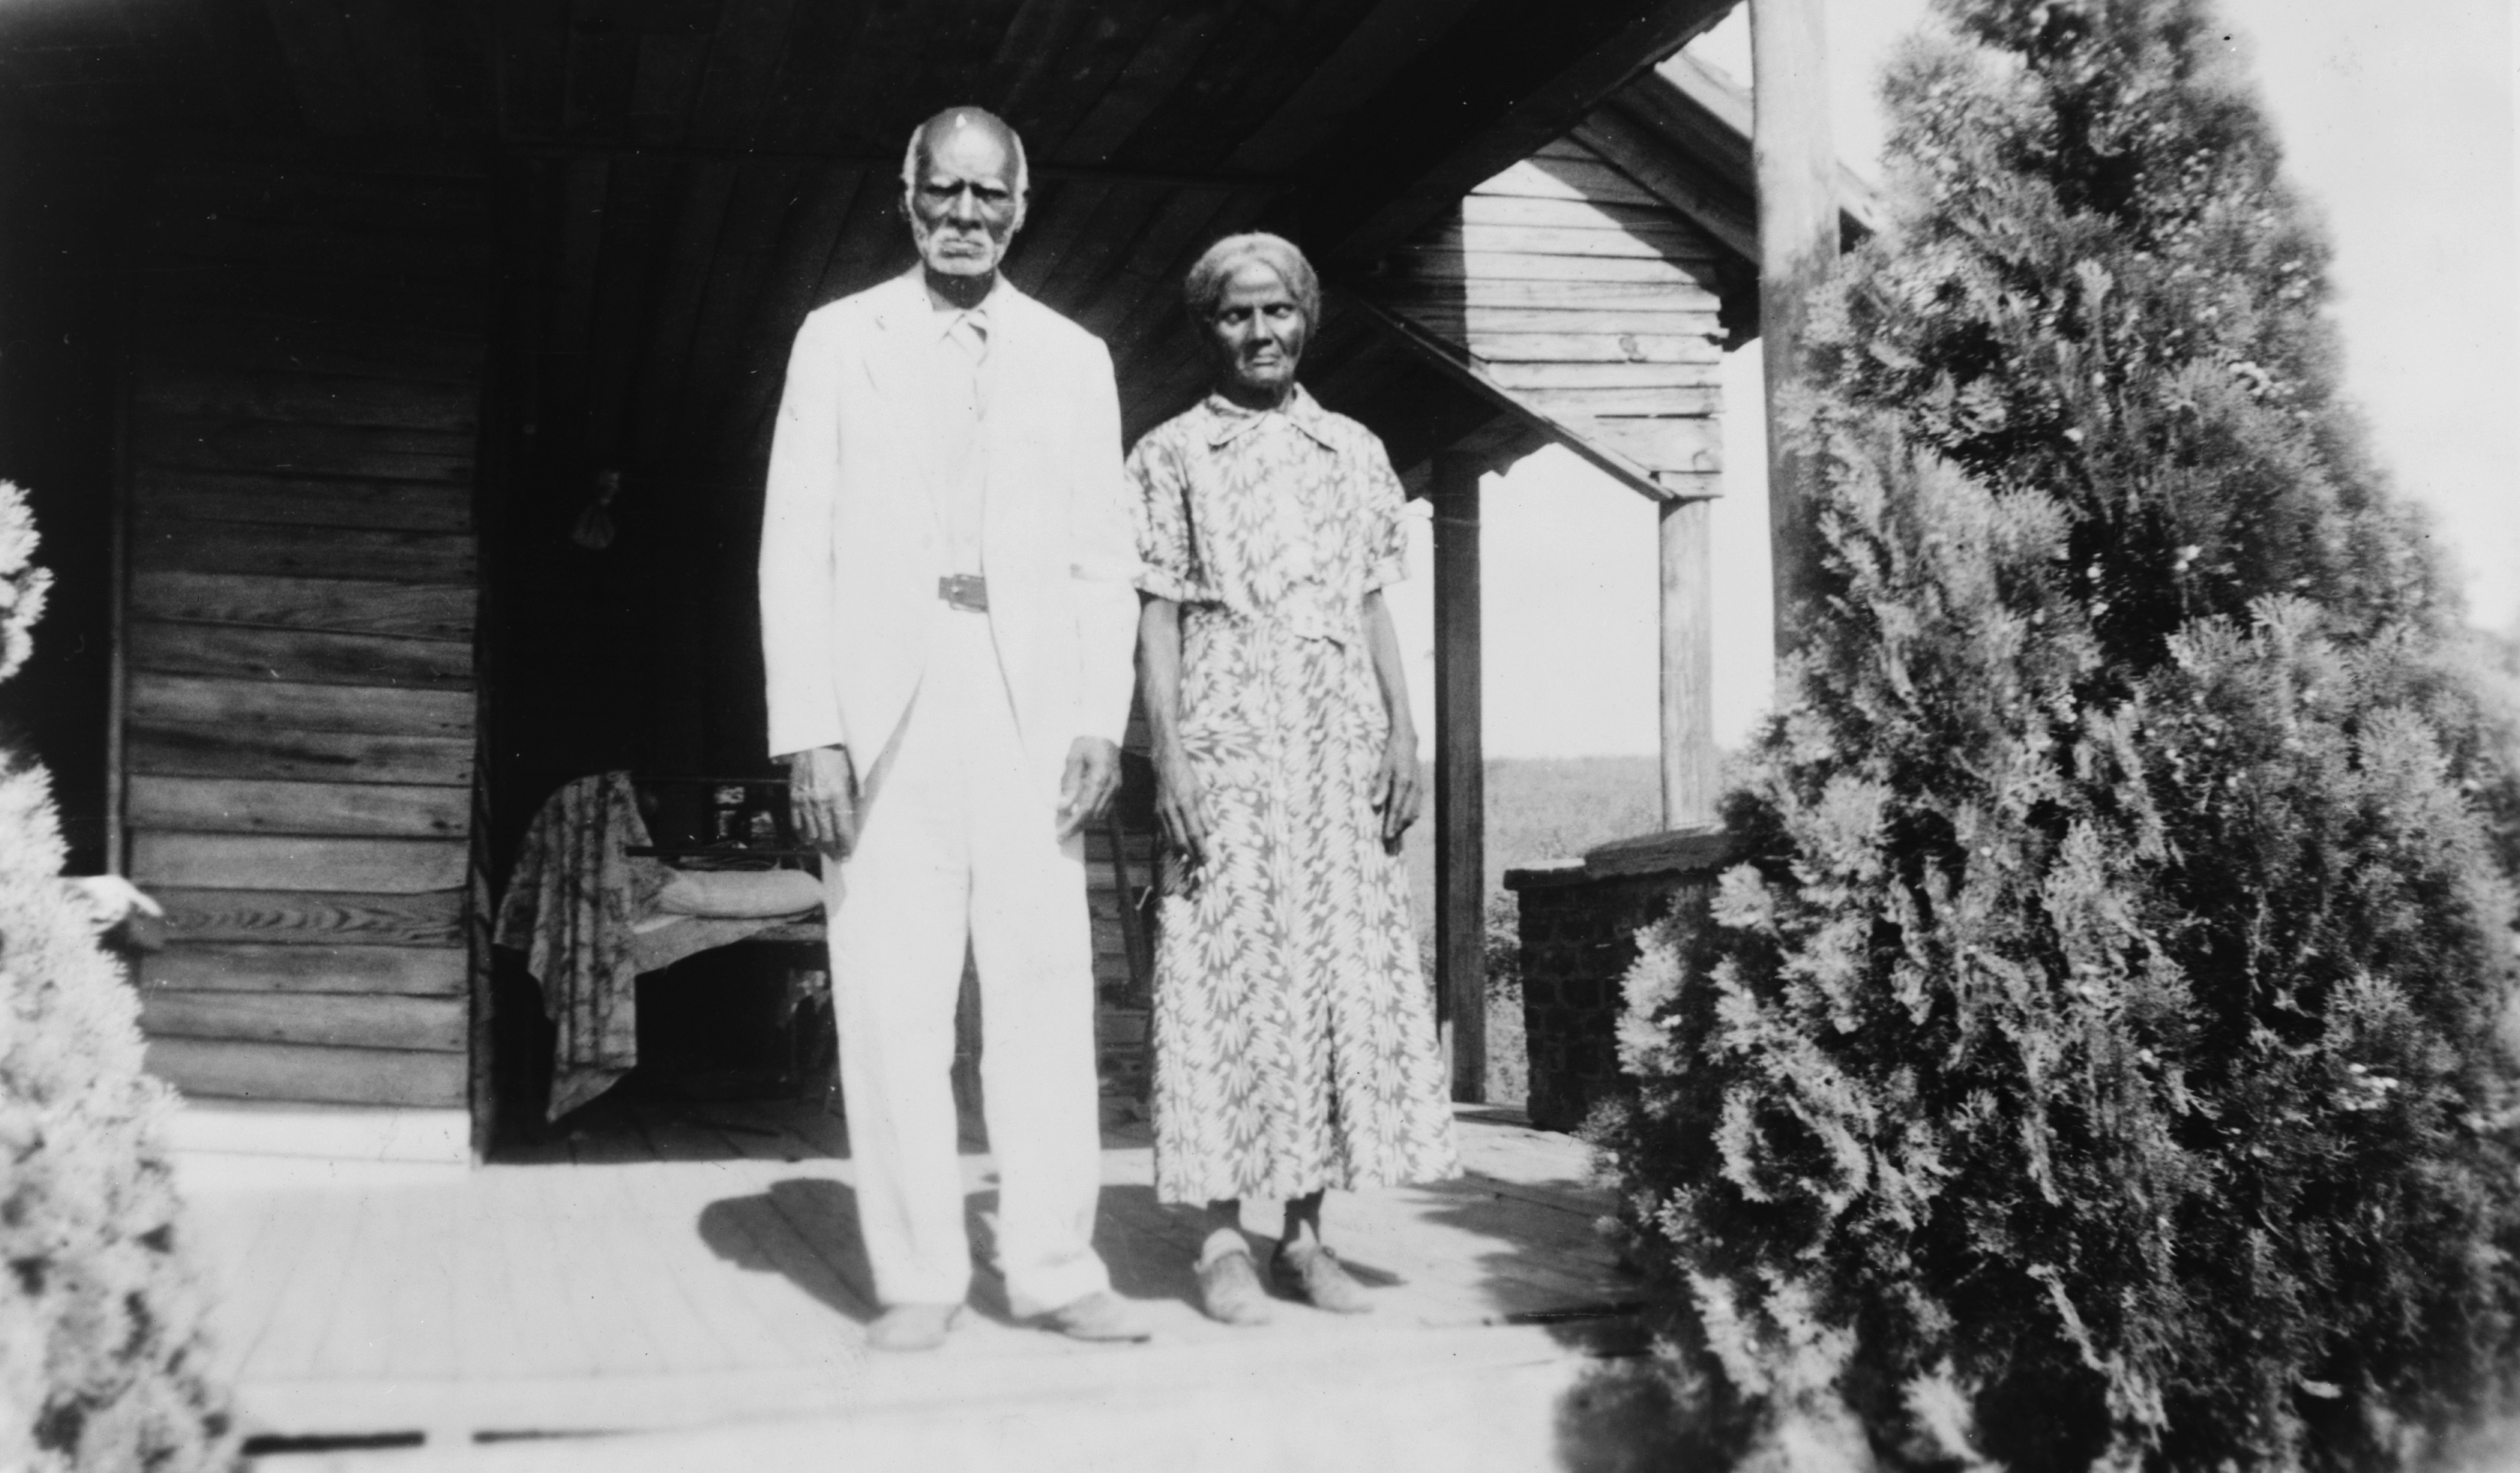
\includegraphics[width=90mm]{./imgs/anderson_minervaedwards_recorte.jpg} \label{img16}
\caption{Anderson e Minerva Edwards}
%\end{minipage}
\end{figure}

\subsection{William Moore, narrativas do Texas, Parte \versal{III}, página 133}
\label{ref197}

``Alguns domingos, nós íamos a alguma igreja. Sempre gostamos de ir para
algum lugar diferente. O pastor branco sempre nos mandava obedecer
nossos senhores e trabalhar duro e cantar, então quando morrêssemos
iríamos para o Céu. O senhor Tom não se importava quando cantávamos nas
nossas choupanas à noite, mas não dava para ele nos pegar rezando.

Parece que os negros têm sempre que rezar. Rezei metade da minha vida.
Algum negro ficava de vigia para cuidar se o senhor Tom estava por
perto, então os outros faziam um círculo no chão da choupana para rezar.
Eles ficavam gemendo, bem baixinho: `Um dia, um dia, um dia esse jugo
será tirado dos nossos ombros'".

\paragraph{Comentário}\quad
{\small
O conjuro reunia crenças e ideias de origem africana e/ou
caribenha. Alguns entrevistados também mencionam ``hoodoo'' ou vodu. No
Sul, os brancos usavam ervas para fazer remédios tradicionais e tinham
muitas superstições, especialmente aquelas que envolviam fantasmas, e os
escravizados conheciam muito bem essa cultura. Mas a natureza das suas
crenças sobre conjuro era distinta das tradições brancas. Ao que parece,
a maioria conhecia ou acreditava no poder dos conjuradores,
ainda que, para alguns, a religião os levasse a rejeitar a
ideia de conjuros ou feitiçaria.
}

\subsection{Emmaline Heard, narrativas da Geórgia, Parte~\versal{IV},~página~259}
\label{ref135}

``Todas as noites, Tio Ned fazia uma enxerga no chão para o papai e
fazia ele ir dormir. Quando ele ia para cama, Tio Ned ficava cuidando
ele com o canto do olho, mas papai fingia que estava dormindo e ficava
olhando o Tio Ned para ver o que ele ia fazer. Depois de um tempo, Tio
Ned tirava uma vassoura e varria bem a lareira, então pegava um cesto e
tirava vários pacotinhos enrolados em pano branco. Para cada pacotinho
que tirava ele dizia `gafanhotos', `aranhas', `escorpiões', `cabeça de
cobra', etc., depois pegava uma tenaz e virava eles na frente da chama
para tostar bem. Noite após noite, ele fazia a mesma coisa até estarem
sequinhos o suficiente, então moía tudo junto para fazer um pó, que ele
colocava em uns saquinhos. Papai tinha medo de perguntar para o velho o
que ele fazia com esses saquinhos, mas ouviu falar que conjurava gente
com eles. Ele conjurou mesmo uma menina, porque ela não dava atenção
nenhuma para ele. Essa menina era muito novinha e preferia conversar com
os homens mais novos, mas Tio Ned ficava sempre arrodeando ela, ajudando
a arar, mas ela sempre mandava ele ir cuidar do próprio trabalho que o
dela ela sabia fazer. Um dia ele disse para ela: `Muito bem, madame, nos
vemos depois. Você não está me vendo agora, mas depois vai se
arrepender'. Quando chegou o almoço, eles saíram do eito e deixaram as
enxadas de pé para saberem onde começar quando voltassem. Quando aquela
menina voltou para a plantação, no instante que encostou na enxada, ela
caiu morta. Dizem que viram Tio Ned esfregando a enxada com conjuro.

Lizzie, minha irmã, foi pega de verdade, e precisou um conjurador velho
para desenfeitiçar ela. Foi assim, menina: Lizzie tinha um pessegueiro
bem bonito, com um galho esticado sobre a trilha, e assim que passava
embaixo desse galho ela ficava o tempo todo doente. O engraçado é que
quando estava na casa dos outros, ela se sentia muito bem, mas no
instante que passava embaixo desse galho, ela começava a passar mal. Um
dia, ela mandou chamar um conjurador. Ele olhou embaixo da casa e, ora,
achou a coisa presa no batente. Parecia um amontoado de panos, flanela
vermelha espetada com agulhas e tudo mais. O conjurador velho disse para
ela que a árvore tinha sido encantada para ela e que o melhor seria
derrubá"-la. Era uma árvore bonita e ela odiou ter que derrubá"-la daquele
jeito, mas ela fez o que ele mandou. Sim, minha filha, não sei se já me
conjuraram ou não, mas às vezes minha cabeça dói e eu fico na dúvida''.

\subsection{``Tio Willis'', narrativas da Geórgia, Parte~\versal{IV},~páginas~173,~174}
\label{ref323}

``Willis foi questionado sobre superstições e respondeu com absoluta
seriedade: `Toda a gente neste mundo tem um espírito que anda atrás de
si e enxerga coisas diferentes. Tive uma visão enquanto dormia
(\ldots{})'

Perguntou"-se a Tio Willis se alguma vez vira alguém ser conjurado. Sua
resposta: `Tem gente no mundo que sabe como se mata o conjuro em
qualquer um, mas ninguém nunca me conjurou. Ouvi dizer que se alguém
conjura você, você pega uma coisa que pode acabar em morte'".

\subsection{Susan Smith, narrativas do Texas, Parte \versal{IV}, página 46}
\label{ref248} 

``Espíritos? Eu costumava ver eles. Tinha medo deles. Às vezes, eles
parecem naturais, mas outras vezes parecem sombras. Se parecem uma
sombra, então você tem que ficar olhando para eles até ficarem naturais.
Se seguir caminhando, eles se juntam no seu lado. Dá para ver eles
quando se olha por cima do ombro esquerdo. Eles deixam o ar morno e
arrepiam os seus cabelos, mas outras vezes eles dão calafrios. Dá para
sentir quando eles estão com você. Estava sentada aqui e vi eles parados
naquele portão. Eles andam por aí igual a quando estavam vivos. Tem quem
diga que não podem cruzar a água.

Eu ouvi falar da boca ruim. Uma velha jogava a boca ruim em você e
chacoalhava a mão e você sofria um acidente antes do fim do dia''.

\subsection{``Tia Irene'', narrativas do Alabama, página 322}

``Tia Irene, você lembra alguma coisa dos conjuradores de antigamente?
`Eu não dou muita confiança para aquela gente. Costumavam dar uma mão
para você agradar a senhora e vendiam água de quieto em garrafão. Água
de quieto era só água normal, mas mexiam nela para que quem bebesse
ficasse calmo e paciente. Os homens arranjavam para dar para as suas
mulheres e fazer elas se aquietarem. Imagino que alguns homens iam
gostar de arranjar um pouco de água de quieto hoje em dia, porque essas
meninas de hoje em dia são muito desbocadas'".

\subsection{Washington Dozier, narrativas da Carolina do Sul, Parte~I,~página~334} \label{ref76}

``Essas coisas que as pessoas chamam de fantasmas, elas são é coisa
ruim. Isso eu sei, o espírito do corpo viaja, e isso é verdade, juro que
é. É claro que nunca vi nada disso e também não tenho medo de nada
dessas coisas. Não dou bola nenhuma para gato preto nem nada disso.
Também não me incomodo com nenhum desses amuletos. As pessoas tinham
seus livros de médico e procuravam nele e usavam o que dizia ali. Não
usavam remédio nenhum que não fosse calomelano e óleo de rícino e
terebintina''.

\subsection{George Leonard, narrativas da Geórgia, Parte~\versal{IV},~página~261}
\label{ref169}

``Naqueles tempos, os mais velhos acreditavam em bruxaria e conjuro e
essas coisas. Eles acreditavam que um velho podia castigar qualquer um
só pegando uma lasca de madeira, cuspindo nela e então atirando na
pessoa. Eles diziam que em duas semanas os vermes iam estar no corpo.

Vi pegarem um gato preto e ensacarem e então levarem o saco e jogarem
numa panela de água fervente com ele ainda vivo. Ai, mas o gato quase
destruía aquela panela tentando fugir. Depois que cozinharem até toda a
carne cair do gato, levavam um dos ossos (não sei qual deles) e
colocavam cruzado em cima dos dentes enquanto murmuravam alguma coisa
baixinho, depois pegavam esse osso e atiravam por cima do ombro direito.
Quando juntavam ele do chão e colocavam no bolso, era para isso dar a
melhor sorte do mundo. Podiam dizer ou fazer tudo que quisessem e o
senhor não tinha como encostar a mão neles''.

\subsection{Jasper Milligan, narrativas da Geórgia, Parte~\versal{IV},~página~252}
\label{ref193}

``Muitos anos atrás, vi uma senhora que foi conjurada nos pés; alguém
colocou alguma coisa no chão para ela caminhar por cima. Bem, ela ficou
com os pés de tal jeito que não conseguia ir da cama até a cadeira. Ela
chamou um velho médico do conjuro para vir tratá"-la e ele esfregou um
remédio nos pés dela, e um pouco depois ele disse para ela que tinha
alguma coisa saindo dos pés dela. Pois, eu vi com os meus próprios olhos
as larvas saindo dos pés dela; mas ela melhorou''.

\subsection{Addie Vinson, narrativas da Geórgia, Parte~\versal{IV},~página~110}
\label{ref271}

```Não lhe contei antes, mas um pedaço desse pátio aqui é conjurado. Um
homem vem todos os dias no começo da manhã e espalha um conjuro no
pátio. Assim que sentei aqui para conversarmos, comecei a sentir uma dor
nas pernas e agora ela já se espalhou por tudo. Eu quis voltar para
dentro de casa. Vem. Vamos sair desse quintal agora mesmo. Rápido!'
Assim que chegou à cozinha, Addie se apressou até o pimenteiro e
espalhou seu conteúdo sobre cada um dos ombros e a cabeça, dizendo: `Uma
coisa quente dessas sempre expulsa o feitiço'".

\subsection{``Tio Henry'' Barnes, narrativas do Alabama, página 23} \label{ref16}

``A senhora me pergunta se a gente sabia alguma coisa de hoodoo? Sim,
senhora, tinha mesmo gente que sabia jogar feitiços nas pessoas. Eu
tinha muito medo deles, sabe? Quando eu estava quase crescido, tinha uma moça
de nome Penny que ficou doente um tempão. Tinha um doutor de conjuro que
fazia uns óleos para tentar curar ela, mas ela não simpatizava, então
ele deixou ela morrer. Depois, um menino de nome Ed tinha uma coisa ruim
no pé que subiu pela perna e deixou ele aleijado. Tinha um doutor de
hoodoo nas bifurcações do rio Tombigbee que vinha cuidar do menino, e
ele mandou todo mundo sair da casa menos ele, Ed e o Diabo. Ele curou Ed
para lá de bem.

Mamãe diz que eu nasci com um olho afiado para ver espíritos e eu
enxerguei alguma coisa que parecia uma vaca sem cabeça. Então mamãe me
fez mexer a banha fresca enquanto derretia, porque isso cura você de ver
os espíritos. Depois que eu mexi a banha, não vi mais eles''.

\subsection{Rosanna Frazier, narrativas do Texas, Parte~\versal{II},~páginas~64--65} \label{ref93}

``Sou cega assim há mais de 40 anos. Um domingo, passei a noite inteira
com um homem e a esposa dele. Eu estava trabalhando de lenhadora na
estrada de Santa Fé em Beaumont, até o Condado de Tyler. Depois que a
gente se levantou e eu fui embora, não andei nem 15, 16 metros quando
ouvi alguém dizendo `Rose, você fez algo que não devia'. `Não, Senhor,
não', eu respondi. E então a voz disse: `Algo vai acontecer com você', e
na manhã seguinte eu estava cega feito um morcego, nunca mais enxerguei
nada.

Tem quem me diga que o motivo foi a neve ou o suor ou a fumaça. Não foi
esse o motivo. Foi esse pé"-virado velho, bem velho, da Luisiana, dizem
que é um conjurador, um desses negros velhos do hoodoo. Ele ficou brabo
comigo na última colheita da ameixa, então fez um pó de cascavel e
passou no meu cabelo, é por isso que eu não enxergo mais nada.

Essa não é a coisa mais malvada que os velhos dos conjuros fazem. Eles
fazem um pó do guizo da cobra e amarram um saquinho de pano com ele para
fazer sortilégios com ele. Pegam um escorpião velho para fazer poção.
Tiram terra do cemitério e então eles falam com a terra, isso deixa você
maluco.

Quando querem botar um conjuro, eles vão escondidos e roubam o cabelo do
pente, ou uma unha da mão ou do pé, ou qualquer coisa natural do seu
corpo, e fazem o hoodoo nela.

Eles fazem um homem de palha ou de barro e enfiam uma agulha na perna,
daí a sua perna dói ou se machuca bem onde deram a agulhada. Se colocam
a agulha no coração, você morre, e não tem como se salvar.

Eles fazem o amuleto para usar em volta do pescoço ou do tornozelo e
fazem o pó do amor também, com cuscuta, a videira do amor que cresce no
mato. Eles fervem as folhas e depois moem. Funciona mesmo, eu já
experimentei''.

\subsection{Amanda Styles, narrativas da Geórgia, Parte~\versal{III},~página~344}
\label{ref260}

``Minha mãe diz que a senhorinha dela era uma bruxa e que se casou, mas
que o marido não sabia que ela era bruxa e que ela saía a cavalo de
noite, transformando o leite das vacas em sangue. Dizem que ninguém
sabia o que fazer, mas em vez de leite elas davam sangue. Então um dia,
uma velha apareceu e disse que uma bruxa estava andando na vaca, e que
para desfazer o feitiço eles tinham que pegar uma ferradura e botar no
fundo da desnatadeira, então o sangue ia virar em leite e manteiga de
volta. Pois bem, foi o que fizeram, e o leite voltou.

Outro homem tinha uma mulher que foi acusada de ser uma bruxa, então ele
cortou a perna dela fora e era uma perna de gato, e quando a mulher
voltou a perna dela tinha sumido.

Dizem que tinha muito conjuro também, ouvi falar muito disso. Meu marido
me contou que uma vez foi ver uma mulher que tinha escorpiões no corpo.
Foi obra do conjurador, que botou sangue de escorpião no corpo dela, e
isso criava mais escorpiões dentro dela. Tiveram que arranjar outro
conjurador para desfazer o feitiço.

Tinha outra família que morava perto da gente que tinha uma filha.
Quando ela morreu, dizem que tinha uma cobra dentro do corpo.

Meu marido diz que foi conjurado quando era menino e tinha que falar com
os braços bem abertos porque não conseguia baixar eles nadinha, não
conseguia nem mexer os braços. Um dia ele encontrou um velho que disse:
`Meu filho, o que é que houve com você?' `Não sei', ele respondeu.
`Então porque não baixa os braços?' `Não consigo'. Então o velho tirou
uma garrafa do bolso e esfregou os braços de cima a baixo até eles
ficarem bem''.

\subsection{Willis Easter, narrativas do Texas, Parte~\versal{II},~páginas~3--4} \label{ref79}

``Nunca estudei conjuro, mas sei que escorpiões e as coisas que se
conjura com eles são um remédio poderoso. Usam cabelo e unha, percevejos
e insetos secos, minhoca e asa de morcego e coisas assim. Mamãe sempre
amarrava uma tirinha de couro ao redor do pescoço dos bebês quando os
dentes estavam nascendo, assim ficava mais fácil para eles. Ela também
usava um sapo seco ou uma lasca de noz"-moscada.

Mamãe sempre me disse que para não levar conjuro, eu tinha que cantar:

\begin{verse}
'Keep 'way from me, hoodoo and witch,\\
lead my path from de porehouse gate;\\
I pines for golden harps and sich,\\ 
Lawd, I'll jes' set down and wait.\\
Old Satan am a liar and conjurer, too\\
If you don't watch out, he'll cunjure you.\footnotemark
\end{verse}

\footnotetext{Tradução: ``Longe de mim, hoodoo e bruxa,/ Desvia meu caminho do asilo dos pobres;/ Eu anseio pelas harpas douradas,/ Senhor, vou só descansar e esperar./ O Velho Satã é mentiroso e conjurador também,/ Se não tomar cuidado, ele
conjura você.''}

Os conjuradores tinham coragem, ah, se tinham. Eles davam pneumonia e
furúnculo e azar. Eu levo um talismã comigo o tempo todo. É um amuleto
enrolado em flanela vermelha. Não sei o que tem dentro. Foi um chefe que
fez para mim.

Eu sei direitinho encontrar água para o poço. Eu pego um galhinho de
árvore que parece um V, daí coloco um prego em cada ponta da forquilha e
na bifurcação. Pego cada uma das pontas e então, se caminho sobre a água
embaixo da terra, o galho vira na minha mão até apontar para o chão. Se
tiver dinheiro enterrado, eu acho do mesmo jeito.

Se você encher um sapato de sal e queimar, isso chama a sorte. Eu uso
uma moeda de dez centavos em um cordão em volta do pescoço e outro em
volta do tornozelo. Isso me protege de qualquer conjurador que quiser me
enganar. A moeda brilha se meus amigos são leais, mas escurece bem quando me
fazem mal.

Para fazer um talismã dos bons, pega serpentária e sassafrás, uma
pedra"-imã pequeninha e enxofre e assafétida, resina e pedra"-lipes, goma
arábica e uma vagem ou duas de pimenta vermelha. Bota em um saco de
flanela vermelha, à meia"-noite na Lua Nova, que funciona sempre''.

\subsection{Compilação de entrevistas com ex"-escravizados de Louise Oliphant, narrativas
da Geórgia, Parte \versal{IV}, páginas 270--72}

``A primeira vez que ouvi falar em conjuro foi quando uma mulher chama
Lucinda machucou a minha irmã. Ela sempre se achou grande coisa e que os
filhos dela eram melhores que os de todo mundo. Bem, a mais velha dela
engravidou, e a Lucinda quase morreu de preocupação. Ela achava que todo
mundo que via estava falando da filha. Um dia, ela passou pela minha
irmã e outra mulher, que estavam rindo e conversando na rua. Lucinda
estava tão preocupada com a filha que achou que estavam rindo dela. Ela
ficou tão braba que amaldiçoou as duas ali mesmo e disse que a vez
dela estava chegando. Minha irmã foi para a casa da outra mulher e
fechou a porta para não ter que escutar a Lucinda. Isso só piorou tudo.

Umas três semanas depois, minha irmã começou a reclamar. Chamamos dois
ou três médicos para ela, mas nenhum deles adiantou nada. Quanto mais
médico a gente chamava, pior ela ficava. Finalmente, todos os médicos
desistiram dela e disseram que não tinham nada que pudessem fazer.
Depois que estava doente fazia dois meses, ela nos contou de um homem
estranho que visitara a sua casa alguns dias antes dela adoecer. Ela
disse que ele visitou três ou quatro vezes. Ela lembrou que quando
visitou depois dela adoecer, ele se ofereceu para ajudá"-la. Os médicos
não tinham adiantado nada e ela estava quase deixando ele cuidar dela
quando a mulher que estava com ela no dia que a Lucinda amaldiçoou as
duas disse que ele era tio"-avô da Lucinda. Ela disse que todo mundo
chamava ele de maior raizeiro da Carolina do Sul. Então minha irmã
lembrou que esse homem tinha pedido água todas as vezes que fizera uma
visita. Ele nunca deixava ela pegar água para ele, sempre ia até a bomba
e pegava ele mesmo. Depois que bombeava uma água bem fresquinha, ele
sempre se oferecia para buscar um balde cheio para ela. Minha irmã não
via nada de errado e deixava ele encher o balde. Foi assim que pegaram
ela.

Ela continuou doente um tempão e mamãe ficou no lado do leito até ela
morrer. Notei que mamãe limpava a boca dela de cinco em cinco minutos,
então um dia perguntei por que ela vivia limpando a boca da minha irmã.
Ela me disse que não era nada, só cuspe. Mas fiquei muito ansiosa por
saber, então eu mesma fui para a cabeceira dela. Finalmente vi o que
era. Umas aranhazinhas estavam saindo pela boca e pelo nariz. Mamãe
achou que isso ia me assustar, é por isso que não queria me deixar ver.

Isso foi na terça"-feira. Naquela sexta, quando ela morreu, uma cobrinha
saiu da testa dela, se empertigou bem reta e pôs a língua para fora para
nós. Um velho que estava sentado ali com a gente pegou a cobra, enfiou
ela em uma garrafa e guardou ela consigo por uma duas semanas, até ela
morrer.

Não ache que Lucinda não conjurou minha pobre mamãe também. Mamãe
adoeceu passado um mês que minha irmã morreu. Depois que descobriu que
os médicos não tinham o que fazer por ela, mamãe arranjou um raizeiro
para cuidar dela. Ele tirou ela da cama e deixou ela firme quase um ano
até Lucinda dobrar a dose. Pobre mamãe, dessa vez ela não conseguiu se
erguer. Ela sofreu e sofreu até morrer. Mas a Lucinda pagou por tudo
isso. Quando mamãe morreu, Lucinda veio ver ela e disse: `tem gente que
está melhor morto mesmo'. A filha de mamãe quis pular em cima dela, mas
alguns dos mais velhos não deixaram.

Lucinda durou um tempão, mas quando caiu, caiu forte. Ela quase
enlouqueceu, ficou doente tanto tempo quanto minha irmã e mamãe juntas.
Ficou tão mal que ninguém nem conseguia entrar na casa dela, todo mundo
dizia que estava colhendo o que tinha plantado. Ela não deixava nem os
próprios filhos entrar na casa. Depois que ficou tão doente que não
conseguia sair da cama, ela gritava e berrava com eles o mais alto que
podia, até eles irem embora. Ninguém teve pena dela, porque todo mundo
sabia toda a maldade que ela tinha feito.

Logo antes de morrer, Lucinda ficou tão mal que todo mundo começou a
dizer que era uma pena ela ter que ficar lá sozinha, então a filha mais
nova e o marido foram morar com ela. A filha tinha medo de ir sozinha.
Quando ela morreu, dava para escutar ela berrando e praguejando até no
lado de fora. Ela repetia: `Tira eles de mim, não fiz nada com eles. Diz
que não machuquei eles, não deixa eles me matarem'. E de repente ela
começava a praguejar contra Deus e todo mundo que conseguia lembrar.
Quando morreu, precisou quatro homens para segurar ela na cama''.

\subsection{``Tia'' Millie Bates, narrativas da Carolina do Sul, Parte~I,~página~47} \label{ref21}

{[}Após descrever atos de violência, ela conta:{]} ``Não demorou muito
depois disso para os espíritos aparecerem por tudo. Quando você saía de
noite, algo começava a assombrá"-lo. Você ficava com tanto medo que quase
corria em disparada sempre que saía de casa no escuro, mesmo se não
fizesse nada. Meu filho, não me pergunte o que eu vi. Depois daquela
matança toda e daquele fogo, você sabe que ia acabar vendo coisas com
todos aqueles espíritos atormentados rondando pela terra. Pois veja, é
assim, quando um homem é morto antes de fazer tudo que o Bom Senhor
pretendia que fizesse, ele volta para cá e tenta encontrar quem lhe fez
mal. Quer dizer, ele não volta ele mesmo, mas o espírito, esse volta e
começa a vagar. É claro que ele não pode fazer nada, então ele só
assusta e assombra as pessoas''.

\subsection{Harriet Collins, narrativas do Texas, Parte~I,~páginas~244--45} \label{ref58}

``Teve umas coisas esquisitas que os brancos não têm como entender. Tem
gente que vê os espíritos, mas eu não consigo. Mamãe aprendeu muito
sobre a cura, tudo que aprendeu com os velhos vindos da África, e também
um pouco do que os índios ensinaram. {[}Quando a Guerra Civil começou,
quase todos os índios já haviam sido removidos para os territórios a
oeste do rio Mississippi. Oklahoma tinha muitos índios, incluindo alguns
que possuíam escravizados afro"-americanos.{]} Se você tinha reumatismo, era
só ferver raiz de canela"-de"-sassafrás e beber o chá. Para fazer o
unguento, você ferve o verbasco e a uva"-de"-rato com alume e sal. Bote
pimenta vermelha no sapato para espantar o resfriado ou enrola sarça em
volta do pescoço. Para curar febre e malária, tem que fazer chá de
erva"-de"-são"-cristóvão, mas tem que colher a raiz na primavera, quando a
seiva está forte.

Quando os dentes começam a nascer nos bebês, tem que pendurar guizo de
cascavel ao redor do pescoço, mas dente de jacará também é bom. Mostra o
dinheiro para a Lua Nova e você tem dinheiro pelo resto do mês. Manda
cinco beijos e mostra o dinheiro e então faz cinco desejos que todos se
realizam. Se comer feijão"-miúdo no Ano Novo, você tem sorte o ano
inteiro.

\begin{verse}
Dose black"-eyed peas is lucky,\\
When et on Hew Year's Day;\\
You'll allus have sweet taters\\ 
And possum come you way.\footnotemark
\end{verse}

\footnotetext{Tradução: ``O tal feijão"-miúdo dá sorte,/ Come ele no dia de Ano Novo;/ Você sempre vai ter batata"-doce/ E os gambás vão vir para você.''}

Quando alguém se corta, eu sempre queimo uns trapos de lã e defumo a
ferida, ou então queimo uma lenha de pinho e pingo o alcatrão na lã
queimada e amarro na ferida. Para dor de cabeça, eu coloco um cataplasma
de raiz"-forte na cabeça, ou um cordão de noz"-moscada em volta do
pescoço.

Se você mata a primeira cobra que vê na primavera, os seus inimigos não
conseguem ganhar nada de você naquele ano. Para uma torção, pega o ninho
de uma vespa"-cavadora e mistura o barro com argila e depois amarra em
volta da torção. Um cordão com moedinha em volta do tornozelo não deixa
a minha perna ficar com cãibra, e chá de raiz"-vermelha é bom também.
Todas essas coisas de cura vieram direto da África, e sempre funcionaram
para mamãe e para mim também''.

\subsection{Silvia King, narrativas do Texas, Parte \versal{II}, páginas 294--95}
\label{ref167}

``O velho Tom tinha uma garrafinha com raízes de feitiço e água com
enxofre. Ele sempre sabia quando um negro ia ser açoitado. Ele enrolava
um cordão em volta dela e dizia: `Por São Pedro, por São Paulo, pelo
Senhor que fez todos nós, não me conte mentiras, talismã, me conte se o
senhor vai açoitar a Mary'. Pois certo como você está aqui, se o talismã
virava para a esquerda, a negra ia ser açoitada, mas se o senhor não
tinha decidido se ia açoitar ou não, o talismã ficava parado e tremia.

Vocês brancos andam pelo mato e sem saber de nada. Você tira as lascas
do lado norte de um pinheiro velho que levou um raio e esquenta eles bem
numa frigideira e queima até só sobrar cinza, então enfia elas em um
saco de papel pardo. Se um oficial lhe pega e você tem que aparecer na
frente do juiz, você pega o saco e sai à meia"-noite e olha para a Lua
com o saco de cinzas nas mãos, mas não pode abrir a boca. No dia
seguinte, você acorda cedo, vai até o tribunal e espalha as cinzas na
porta de entrada. A incomodação com a lei, ora, ela se desfaz igual
aquele raio desfez aquela árvore.

O cogumelo"-do"-mel é forte como poucos. Se você mastiga ele e cospe em
volta da pessoa de quem quer alguma coisa, você consegue. Dá para
conseguir mais dinheiro, um emprego, quase tudo. Eu tinha um osso de
gato preto também, mas não sei onde foi parar''.

\subsection{Wash Wilson, narrativas do Texas, Parte \versal{IV}, página 198}
\label{ref301}

``Não tinha instrumento musical. A gente pegava pedaços de costela de
ovelha ou queixo de vaca ou um pedaço de ferro, com uma chaleira velha,
ou uma cabaça oca e uma crina de cavalo para fazer o tambor. Às vezes,
pegavam um pedaço de tronco de árvore, escavavam ele e esticavam uma
pele de carneiro ou de bode para ser o tambor. Eles tinham de menos de
meio metro até quase um metro e meio de altura, e de meio metro até
quase dois de largura''.

\begin{figure}[]
\centering
 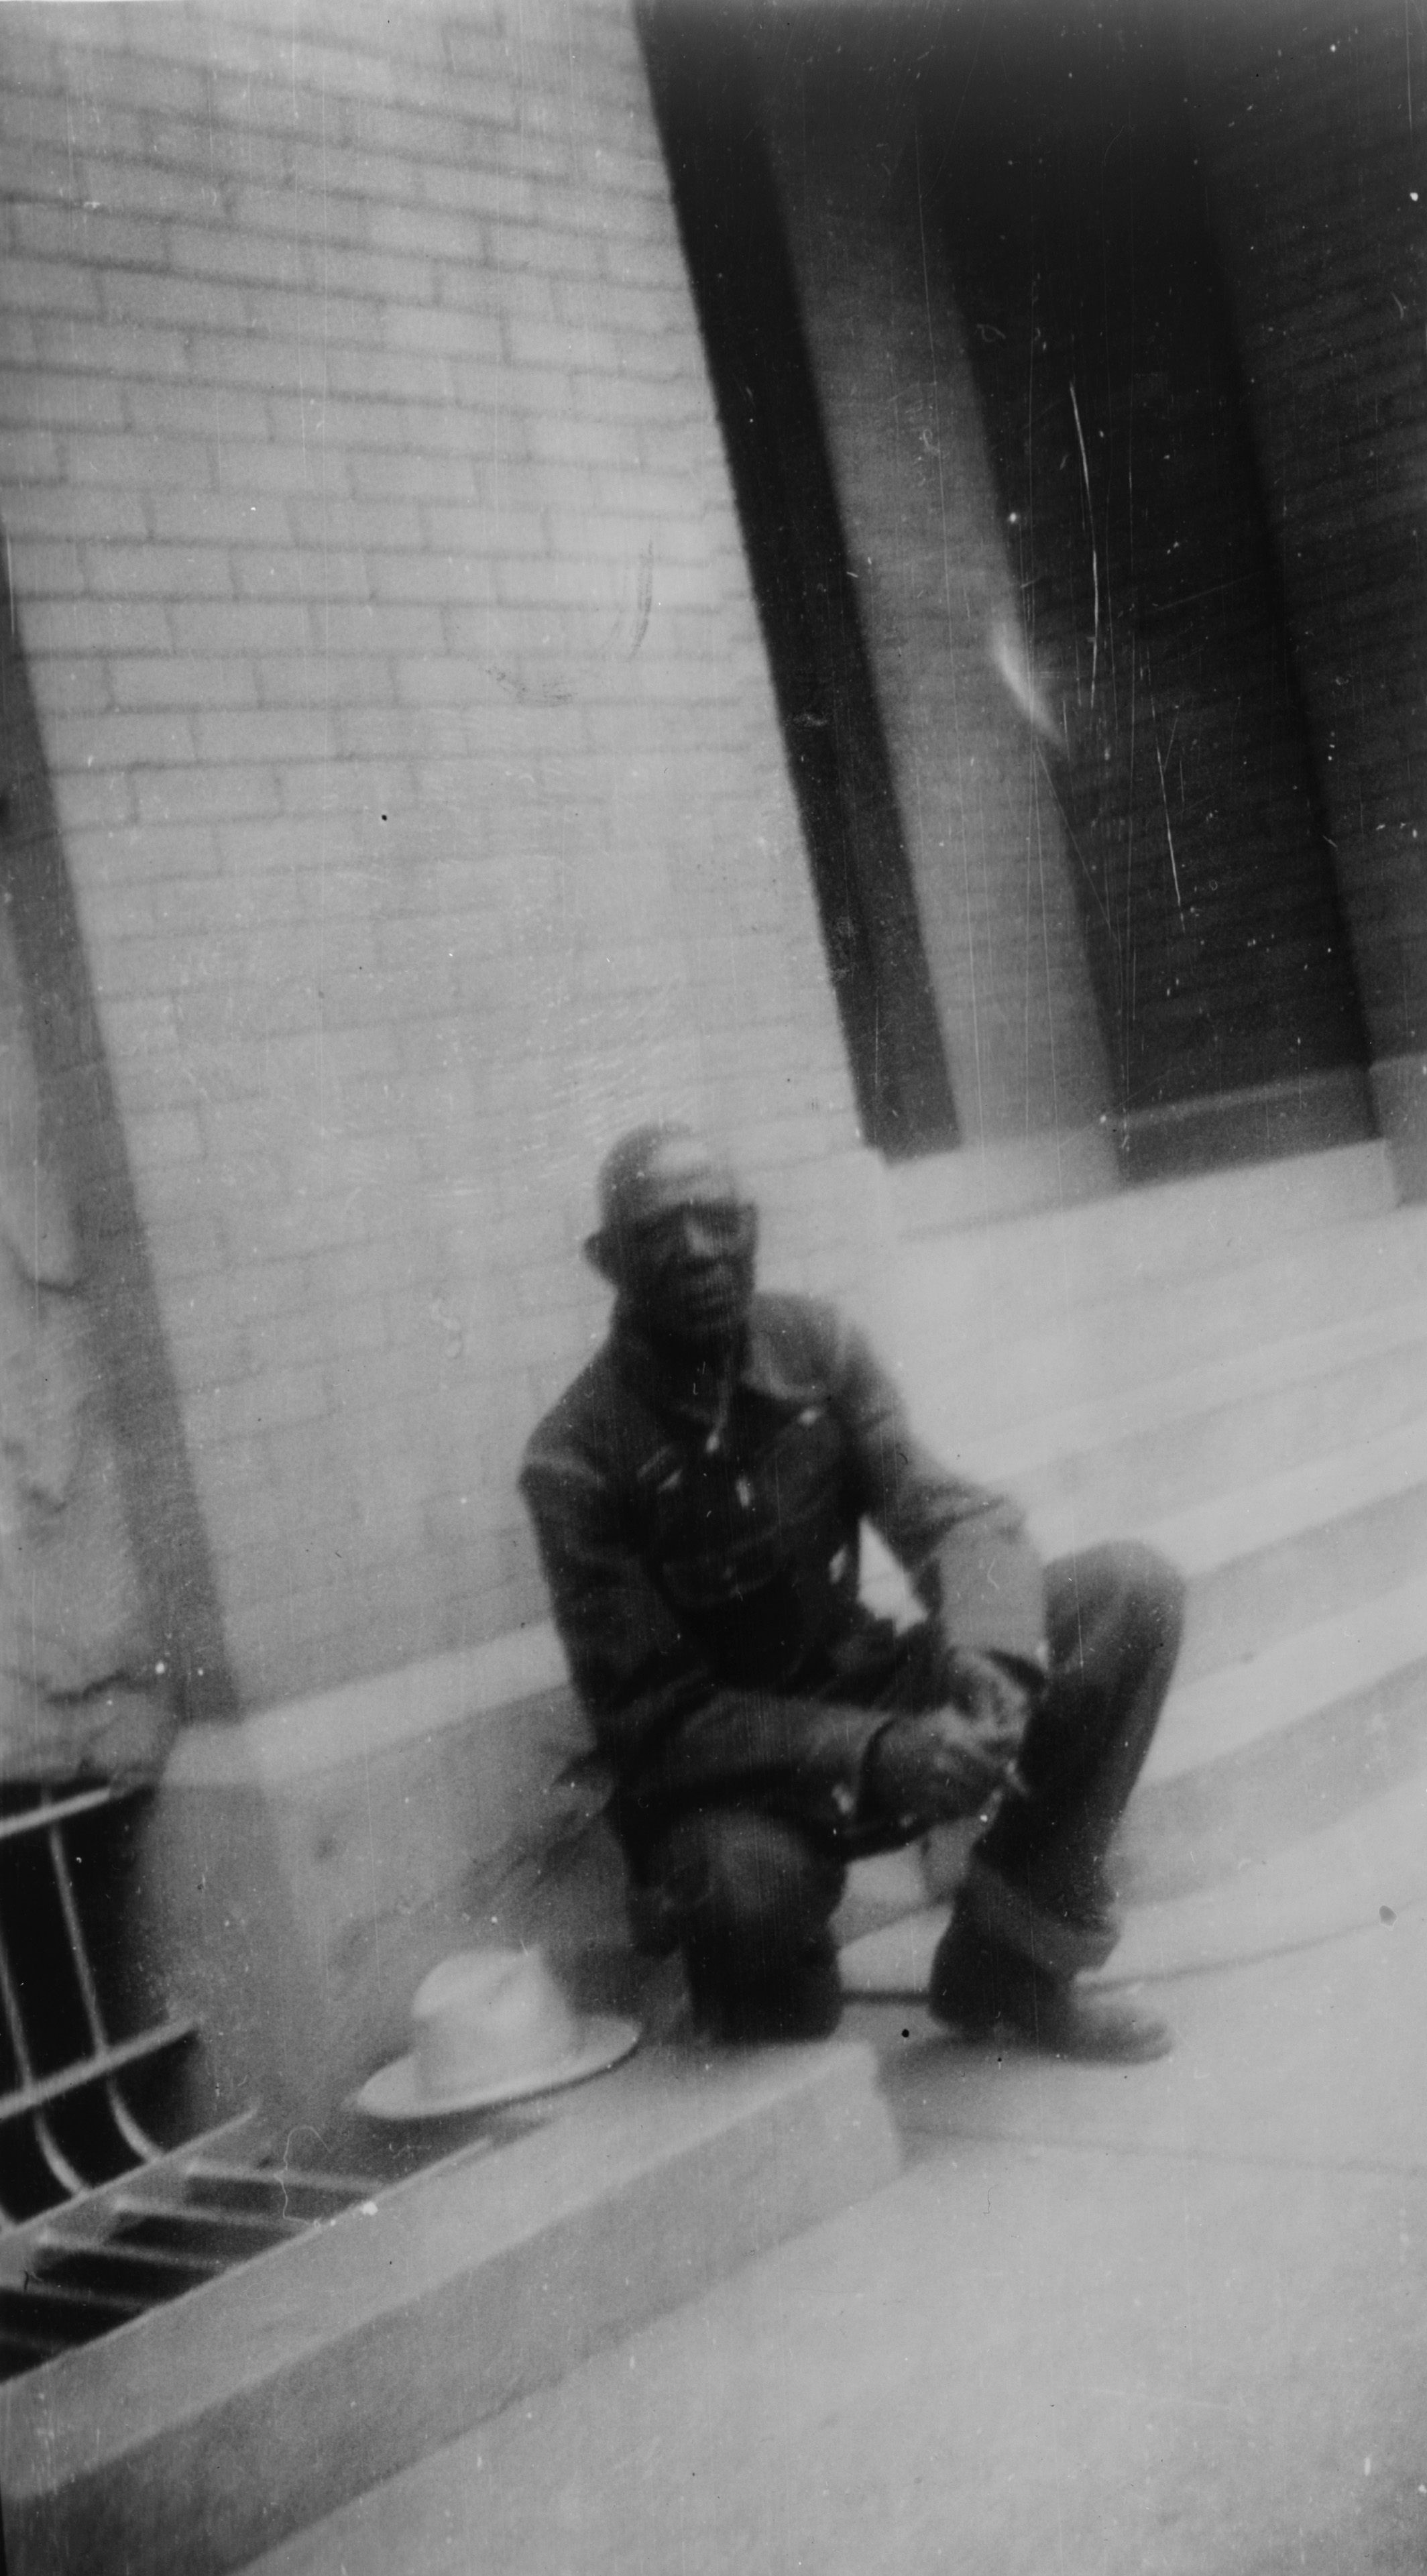
\includegraphics[width=90mm]{./imgs/washwilson_recorte.jpg} \label{img17}
\caption{Wash Wilson}
\end{figure}





\pagebreak
\thispagestyle{empty}

\begin{absolutelynopagebreak}
\begin{vplace}
\begin{figure}[H]
\begin{adjustwidth}{-1.8cm}{}
  %\centering
  \vspace*{-2cm}
  %\hspace{-0.5cm}
  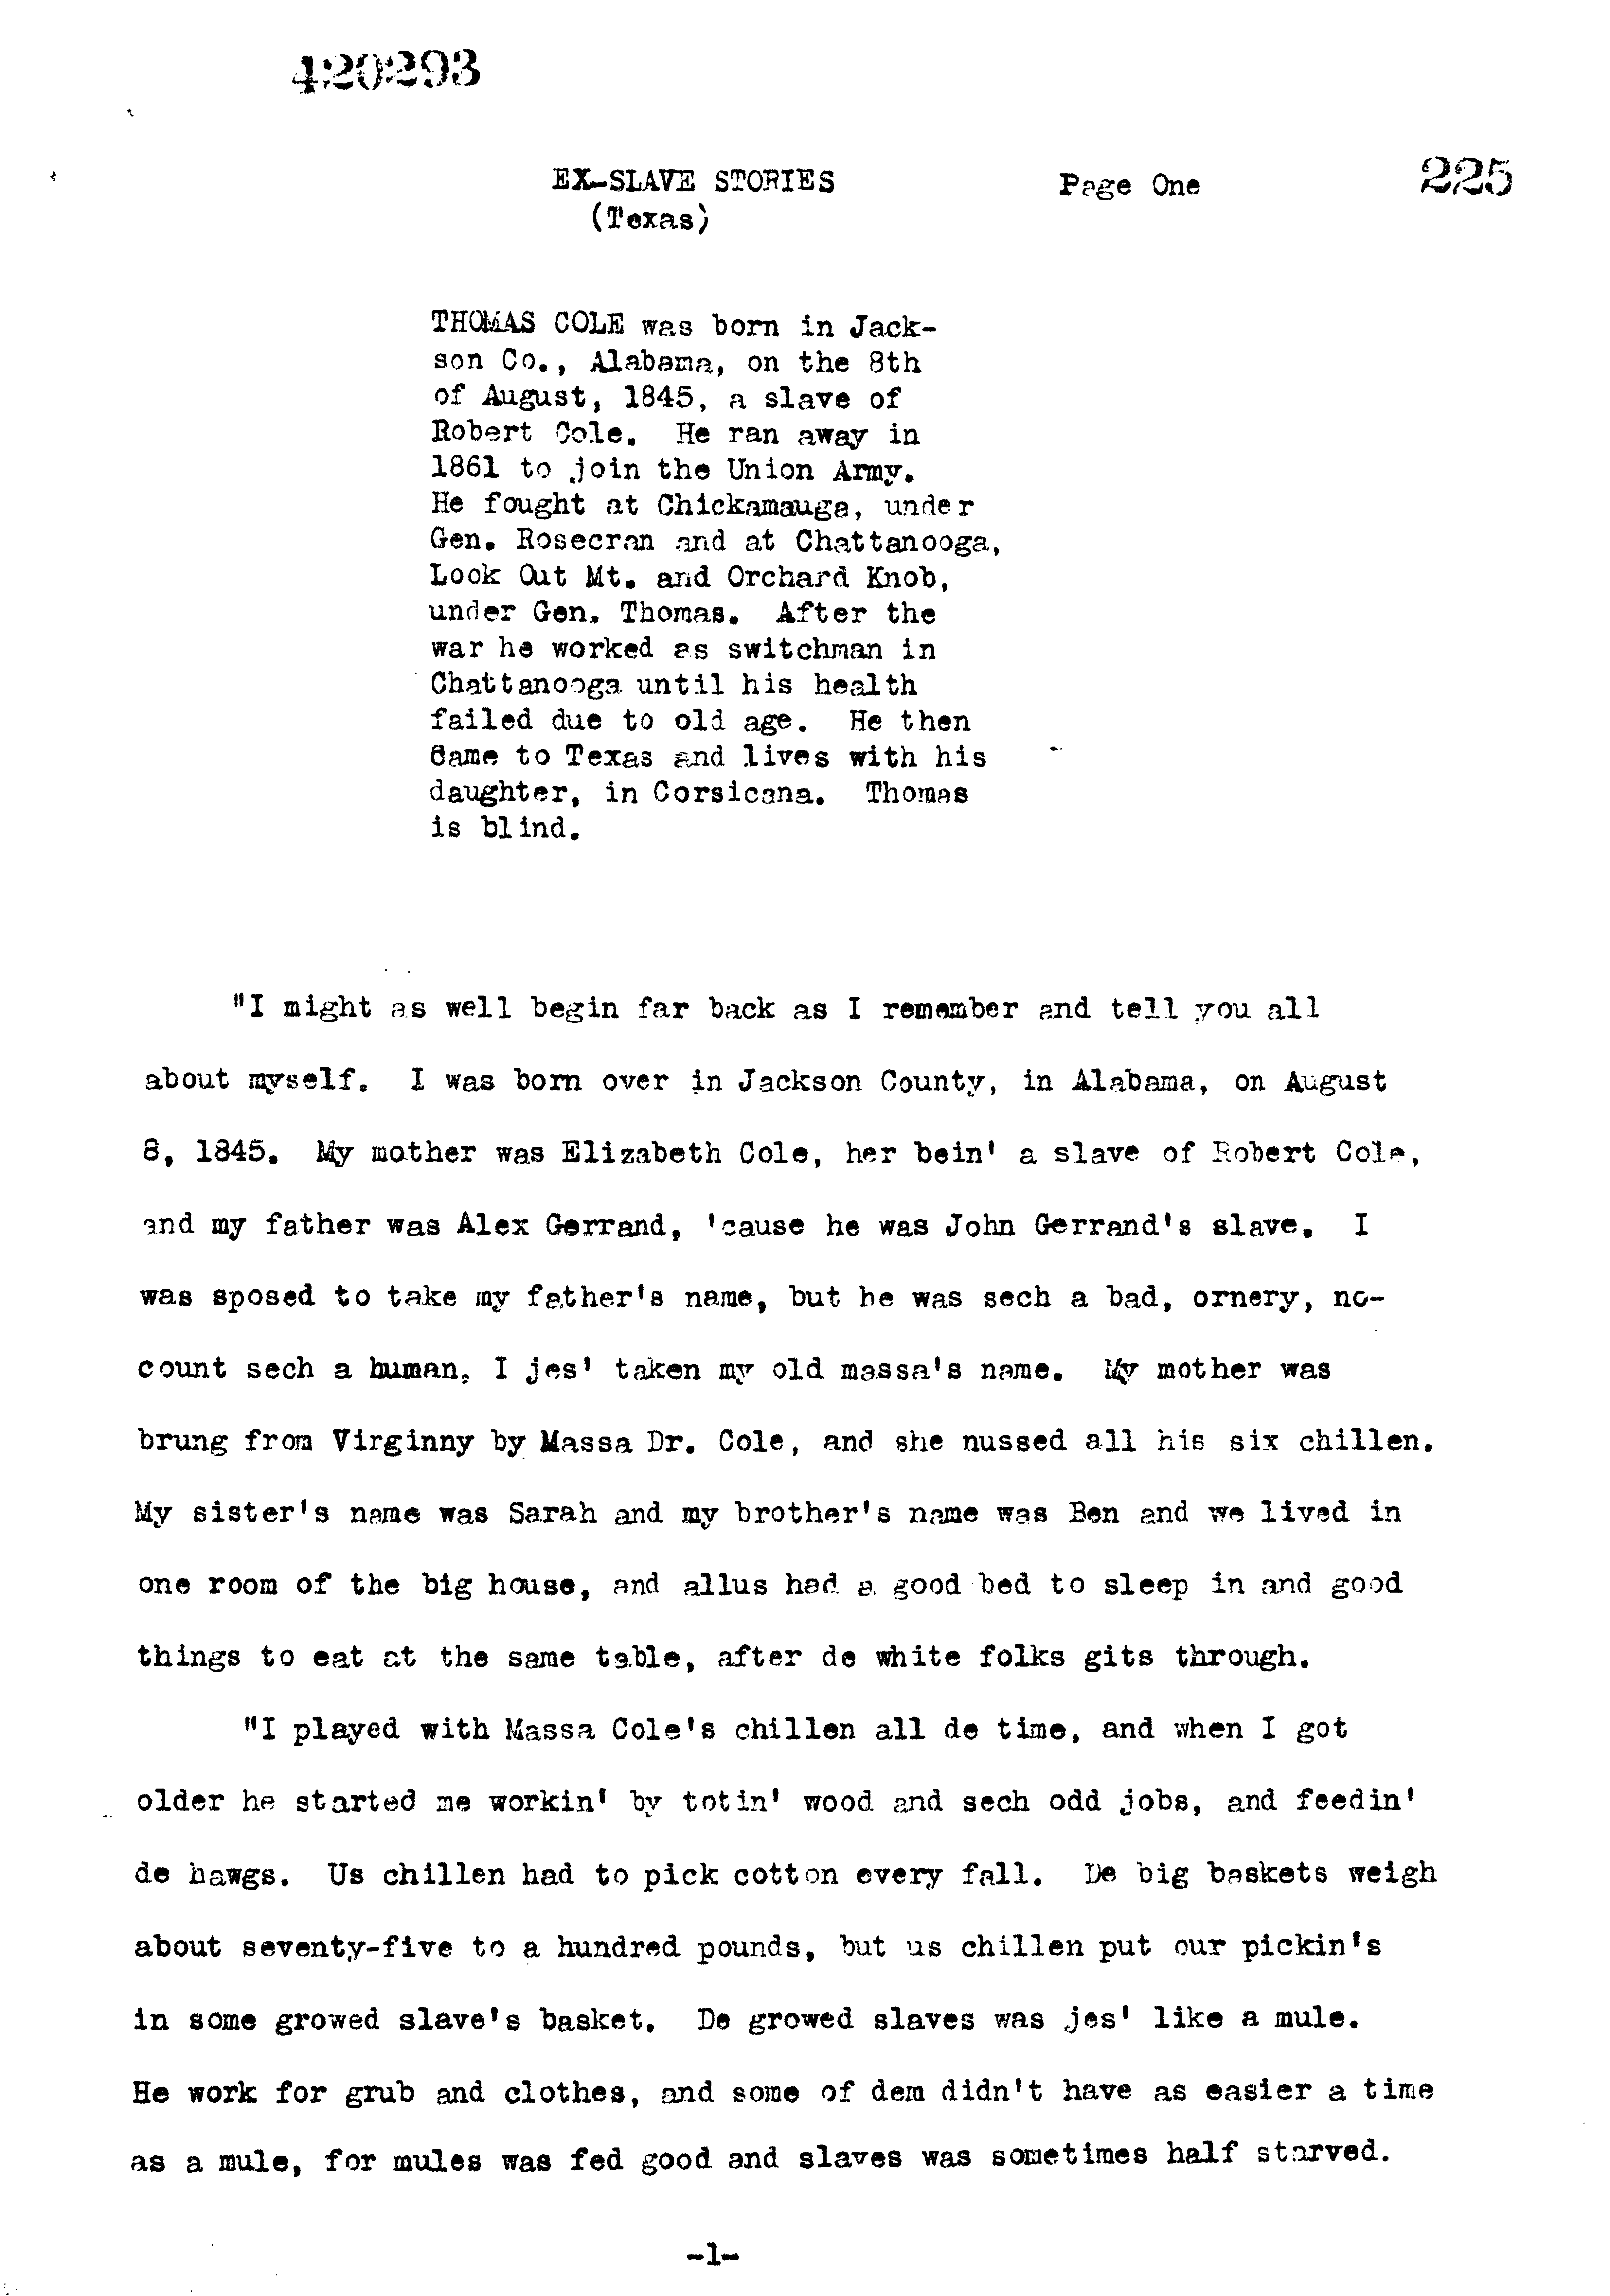
\includegraphics[width=130mm]{./imgs/Cap7.jpg}  
  %\hfill
\end{adjustwidth}
  \caption{Thomas Cole, narrativas do Texas, Parte \versal{I}, página 225}
\end{figure}
\end{vplace}

\end{absolutelynopagebreak}

\chapter{Resistência}
%\addcontentsline{toc}{chapter}{{\large\versal{VII.}} Resistência}
%\hedramarkboth{Resistência}{}

\subsection{Thomas Cole, narrativas do Texas, Parte~I,~páginas~228--30} \label{ref57}

{[}Viveu em situação de escravidão no Condado de Jackson, Alabama. Ele elogia seu senhor por não praticar o açoite, mas depois que seu
senhor morreu:{]} ``Pensei comigo mesmo, aquele Sr. Anderson, o feitor,
ele vai me lascar com o bacalhau na primeira chance que tiver, mas
decidi que ele não ia ter chance nenhuma, porque eu ia fugir na primeira
chance que eu tivesse. Não sabia como sair de lá, mas ia para o Norte,
onde não havia senhores de escravos. (\ldots{})'' {[}As rações foram
reduzidas durante a guerra, então:{]} ``Um dia, ele {[}o feitor{]} me
chamou e disse para não me afastar muito da fazenda, mas mandou trazer
alguma carne. Essa era a chance que eu estava esperando, então quando
chegamos na zona de caça e o líder nos dispersou, disse para ele que eu
e mais outro homem iríamos para o Norte e daríamos a volta em torno do
rio, para nos encontrarmos de novo lá pelo pôr"-do"-sol. Atravessei o rio
e fui para o Norte, estava indo para a terra livre onde não tem
escravos. Viajei o dia inteiro e a noite inteira também rio acima,
seguindo a estrela polar. Várias vezes achei que os cães de caça estavam na
minha pista e comecei a me apressar. Estava tão cansado que mal
conseguia me mexer, mas deu para apertar o passo.

Passei o tempo todo torcendo e rezando para encontrar com aquela tal de
Harriet Tubman, a negra que levava os escravos para o Canadá. Ela sempre
viajava na ferrovia subterrânea {[}\emph{underground railroad}{]}, é assim que
chamavam, viajava de noite e se escondia de dia. Ela tirava eles do Sul
às escondidas e eu acho que ela era uma mulher muito corajosa.

Comi nozes e matei uns coelhos"-do"-pântano e peguei alguns peixes. Eu fiz
uma fogueira, caminhei quase um quilômetro e me escondi no mato até
sobrar só o carvão, então assei o peixe e o coelho. Passei o tempo todo
tremendo, com medo de me pegarem, mas estava quase morrendo de fome.
Coloquei o resto do peixe na minha boina e segui a estrela polar naquela
noite, então me escondi no matagal no dia seguinte. No fim da tarde,
escutei uns tiros. Dessa vez fiquei assustado, ah, se fiquei. Estava com
medo de entrar e com medo de sair, mas parado ali ouvi dois homens
chamarem: `Mãos para cima, menino. O que você está fazendo?' Eu
respondi: `Hã, hã, não sei. Vocês não vão me levar de volta para a fazenda,
vão?' E eles: `Não. Você quer lutar pelo Norte?' E eu disse que lutava,
porque eles falavam feito nortistas. A gente caminhou noite e dia e
chegou ao acampamento do General Rosencrans. Acharam que eu era espião
do Sul. Me fizeram tudo que foi pergunta e disseram que iam me açoitar
se não contasse o que eu estava espiando. Finalmente acreditaram em mim
e me botaram para ajudar com os canhões. Eu me senti importante, mas não
sabia o que {[}o perigo{]} tinha pela frente, pois acho que teria fugido
de novo''.

\paragraph{Comentário}\quad
{\small
Thomas Cole praticou formas de resistências particularmente
dramáticas e eficazes, mas ele não estava sozinho. Os escravizados
ocasionalmente atacavam ou matavam feitores ou proprietários e a
violência irrompia nas fazendas isoladas comuns no interior do sul dos
Estados Unidos. Durante a Guerra Civil, controlar os negros tornou"-se
mais difícil, especialmente quando elementos do Exército da União
invadiam ou ocupavam áreas próximas. Cerca de 150 mil pessoas que
fugiram do cativeiro se juntaram ao Exército da União, lutando para
destruir a escravidão e a Confederação sulista rebelde.

Mas a maior parte da resistência não era tão visível nem tão
dramática. A chance de uma rebelião ter sucesso no Sul era mínima, e a
maioria dos escravizados resistia de modo que pudessem melhorar seus
cotidianos e aumentar sua força e sua coragem para continuar a viver.
Resistir à propaganda dos senhores e ao sistema escravocrata na própria
mente não eram questões triviais. A resistência mental e emocional
era essencial para a sobrevivência e formou a base para o
desenvolvimento de outras esperanças. Boa parte da resistência também se
manifestava em roubos, reuniões e comunicações secretas ou diversos
tipos de embuste.
}

\subsection{Wash Wilson, narrativas do Texas, Parte~\versal{IV},~página~198}
\label{ref302}

``Quando os negros começam a cantar \emph{Steal Away to Jesus} {[}Fuja para
Jesus{]}, isso significa que vai ter um culto religioso naquela noite.
Esse é o significado do culto. Antes e depois da liberdade, os senhores
não gostavam dos cultos religiosos, então naturalmente a gente se
escapulia de noite, lá nas baixadas ou onde fosse. Às vezes, a gente
cantava e rezava a noite inteira''.

\subsection{Mary Reynolds, narrativas do Texas, Parte~\versal{III},~páginas~240--41}
\label{ref223}

``Uma vez, minha mãe e meu pai levaram eu e Katherine às escondidas, de
noite, para rezar e cantar em outra fazenda. Um negro de barba branca
nos disse que chegaria um dia em que os negros seriam escravos só de
Deus. Nós rezamos pelo fim da Tribulação e o fim das surras e para os
sapatos caberem nos nossos pés. Rezamos que os negros tivessem tudo que
quisessem comer, especialmente carne fresca. Alguns dos mais velhos
disseram que a gente tinha que aguentar, porque era tudo que dava para
fazer. Alguns disseram que ficariam contentes em morrer, porque
preferiam apodrecer embaixo da terra do que apanhar. O que eu mais
odiava era quando me batiam e eu não sabia por que estavam me batendo, e
eu odiava que me tiravam a roupa e me deixavam pelada como no dia em que
nasci.

Na volta daquela reza, achei que tinha escutado os cães de caça e alguém
a cavalo. `Mãe, acho que são os cães', eu disse. `E eles vão nos comer'.
Dava para ouvir as cadelas e os cachorros velhos uivando. Mamãe prestou
atenção. `É mesmo, os cachorros estão correndo, Deus nos acuda!', ela
disse, então ela e papai conversaram e nos levaram até um canto da
cerca, onde nos colocaram contra o cercado e disseram para não se mexer,
e que se alguém chegasse perto, não era para respirar alto. Eu e
Katherine ficamos lá paradas, de mãos dadas, tremendo tanto que mal se
aguentava de perto. Ouvimos os cães se aproximando, mas não nos mexemos.
Eles foram atrás dos meus pais, mas eles deram a volta nas choupanas e
entraram. Mamãe diz que foi a graça de Deus''.

\begin{figure}[]
\centering
 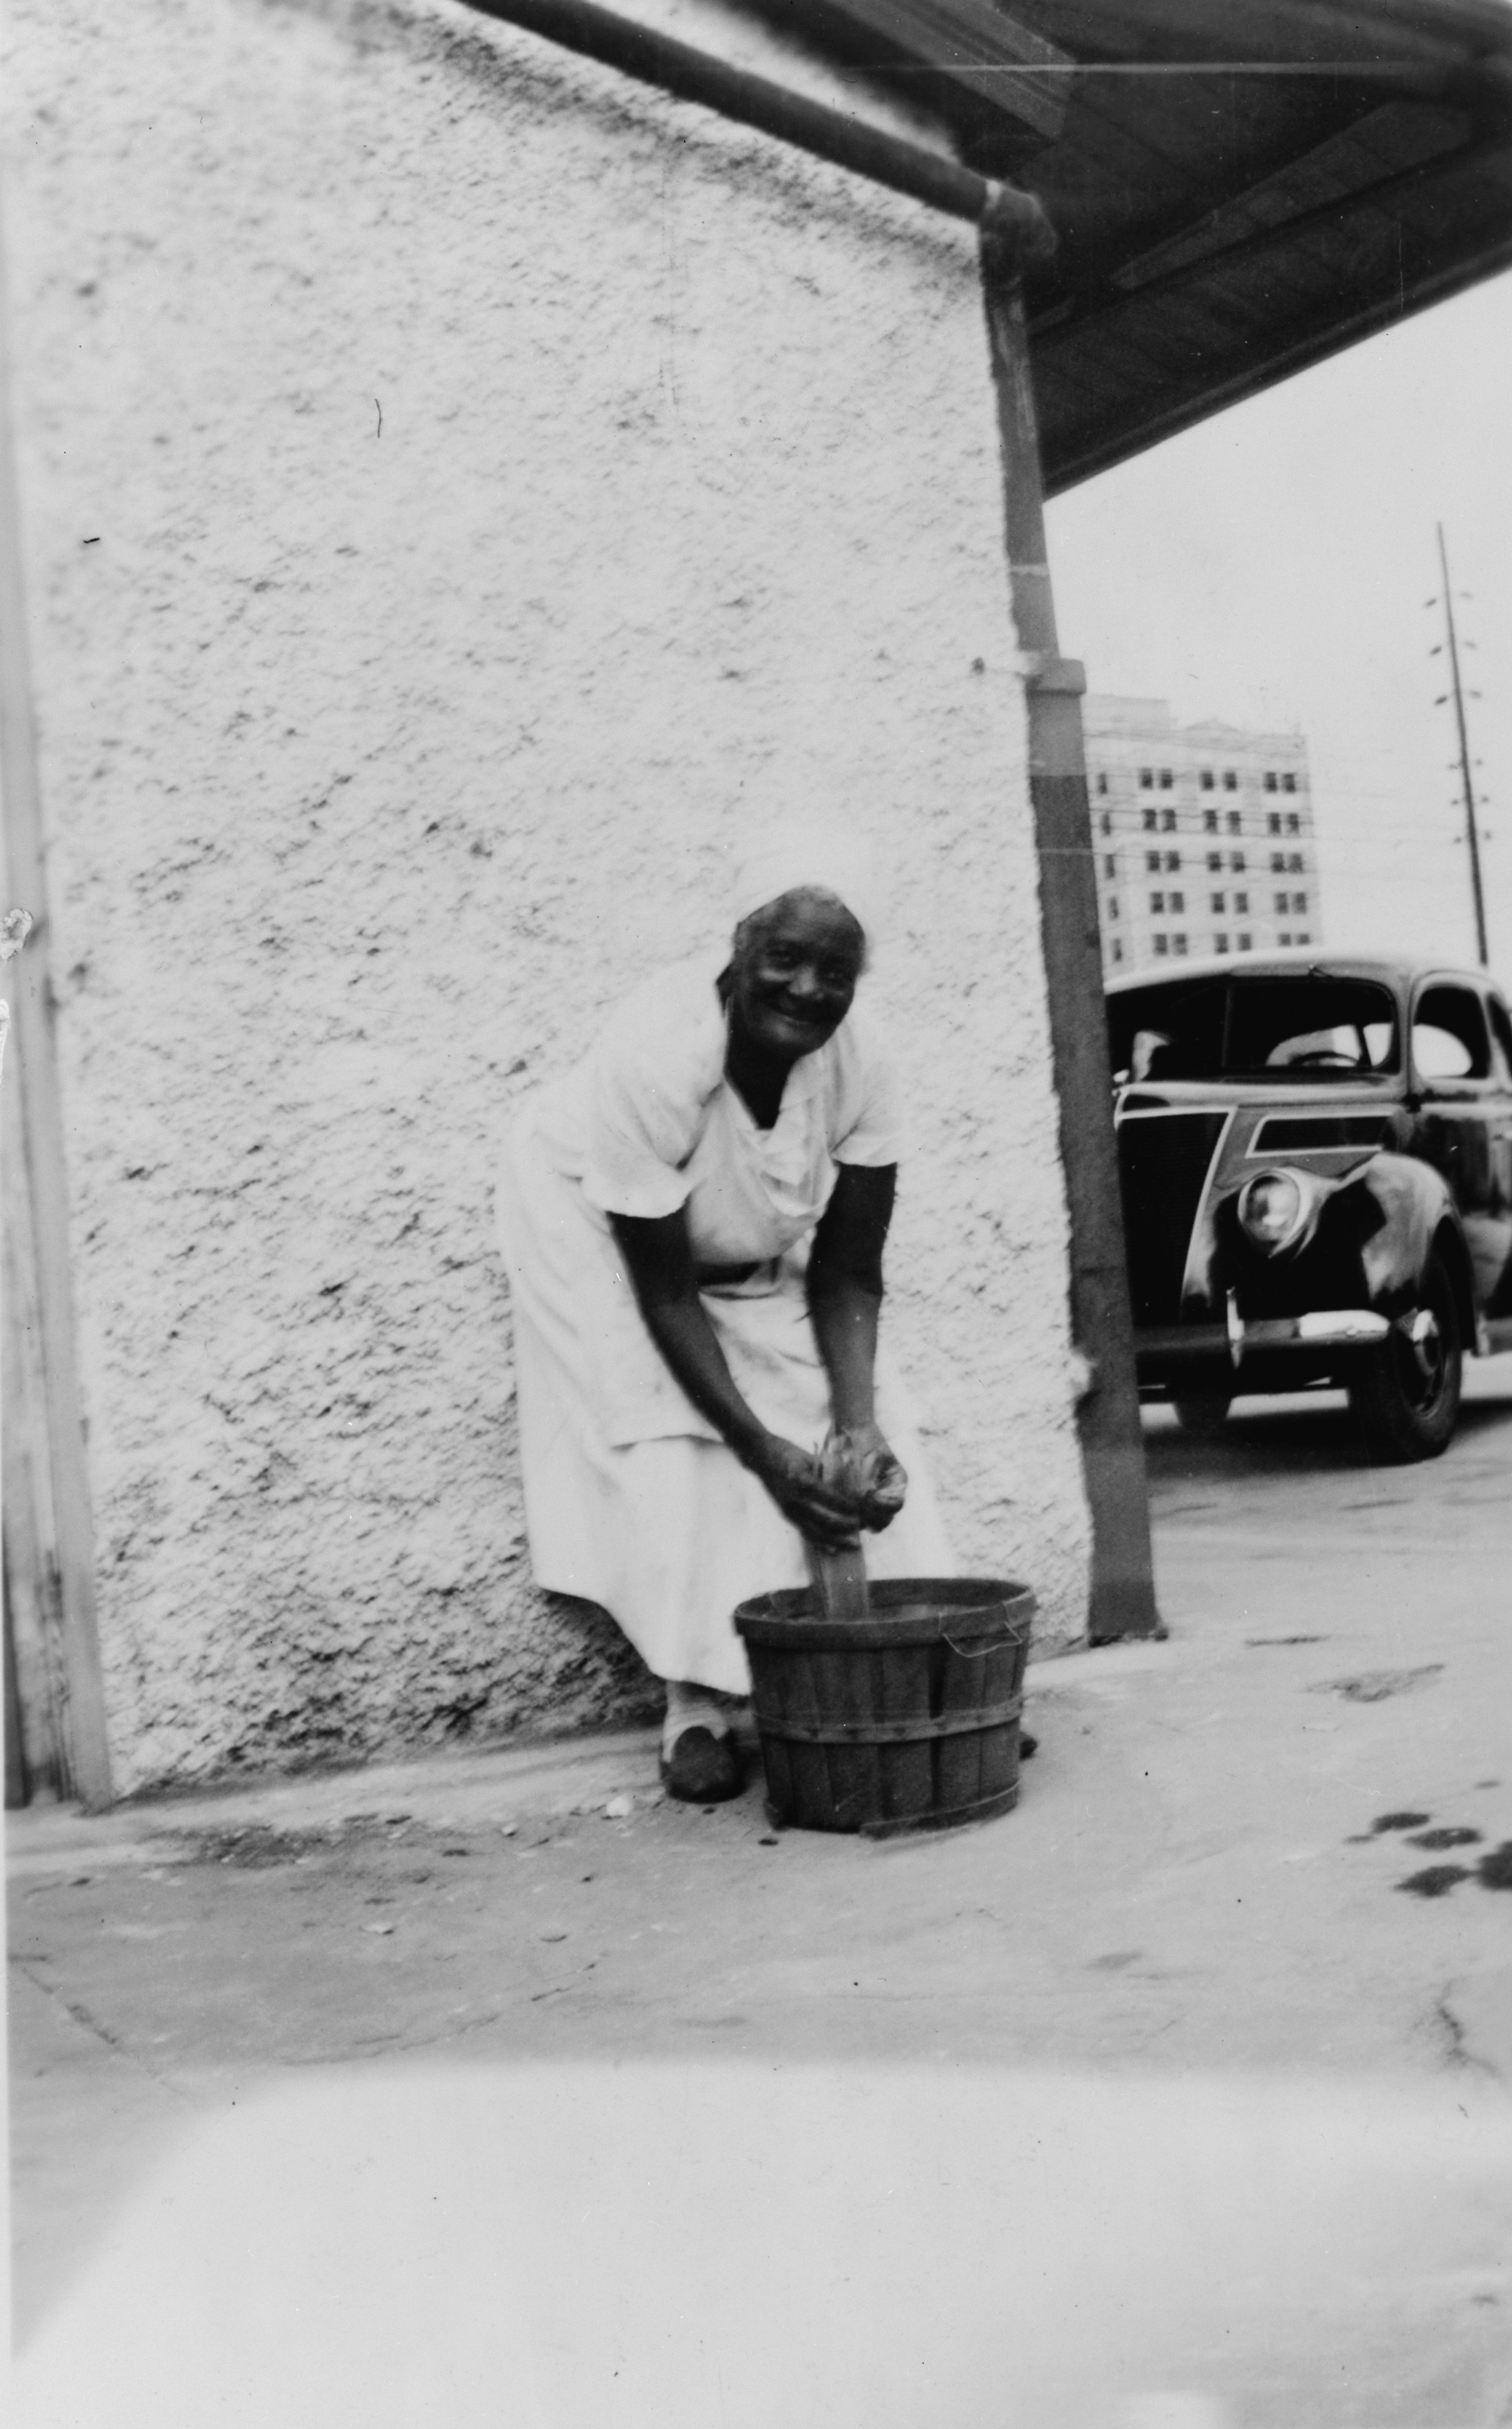
\includegraphics[width=90mm]{./imgs/ellenbutler_recorte.jpg} \label{img18}
\caption{Ellen Butler}
\end{figure}

\subsection{Ellen Butler, narrativas do Texas, Parte~I,~página~177} \label{ref41}

``O senhor nunca nos deixava ir à igreja, mas tinha uns buracões no
campo onde os escravos se abaixavam para rezar. Eles faziam assim porque
os brancos não queriam que eles rezassem. Eles costumavam rezar pela
liberdade.

Quando os brancos saíam, eles escreviam na farinha grossa e na fina com
os dedos. Assim, eles sabiam se a gente roubava a farinha. Às vezes,
eles pegavam um pau e escreviam na frente da porta, então se alguém saía
e pisava na escrita, o senhor sabia. Foi assim que a gente aprendeu a
escrever''.

\subsection{William McWhorter, narrativas da Geórgia, Parte~\versal{III},~páginas~97,~98}
\label{ref192}

``Nenhum dos nossos negros nunca soube o suficiente sobre o Norte para
fugir tão longe. Como eu lhe contei, alguns fugiam depois de uma surra
muito ruim, mas eles só se escondiam no mato. Alguns voltavam em
seguida, outros não. Ninguém sabia onde foram parar os que não
voltaram''.



\subsection{Kitty Hill, narrativas da Carolina do Norte, Parte~I,~páginas~424--45}
\label{ref146}

``Quando a gente era criança, mamãe contava para nós histórias de
patrulheiros pegando negros e surrando eles e como alguns dos homens
conseguiam correr e fugir dos patrulheiros. Tinha uma canção que
cantavam, era assim: Sim, senhor! Rá! Rá! Eu quero lhe contar a canção,
lá vai: `Tem quem diga que negro não rouba, peguei dois no meu milharal.
Um tinha um alqueire, um tinha um celamim, um tinha espigas penduradas
do pescoço. Corre, negro, corre, o patrulheiro vai pegar. Corre, negro,
corre, como correu no outro dia'.

Minha mãe diz que sempre foi bem tratada. Sim, ela disse que eram bons
para ela na Virgínia. Mamãe diz que os escravos na fazenda dos
Jefferson, na Virgínia, roubavam os cavalos para ir aos bailes de noite.
Uma vez, um cavalo que eles roubaram para ir ao baile caiu morto e
tiveram que carregar ele de volta. Mamãe ria muito disso. (\ldots{})

Mamãe diz que os escravos eram proibidos de fazer cultos onde ela morava
na Virgínia. Viravam as panelas para matar o barulho e faziam os cultos
à noite. Colocavam uns negros de vigia para soar o alarme se vissem os
brancos chegando. Eles estavam sempre cuidando os patrulheiros. Eles não
podiam ter nada de educação, minha mãe não sabia ler nem escrever
nada''.

\subsection{George Womble, narrativas da Geórgia, Parte~\versal{IV},~página~185}
\label{ref310}

{[}Eles nunca recebiam comida o suficiente.{]} ``Se a comida acabava
antes da próxima ração, eles esperavam até a noite e então um ou dois
iam até a casa de farinha, onde guardavam a grossa e a fina. Depois que
conseguiam entrar, eles pegavam uma broca e faziam um furo no barril de
farinha grossa. Um segurava o saco enquanto o outro pegava um pedaço de
pau e mexia no buraco aberto pela broca para fazer a farinha correr
livre. Depois que os sacos enchiam, a gente tapava o furo e executava
uma fuga às pressas. Às vezes, quando queriam carne, eles iam até o
defumadouro e roubavam um presunto ou então iam até o chiqueiro, onde os
porcos ficavam, e levavam um leitão. Quando chegavam à floresta com o
animal, eles o esfolavam e limpavam (ele era morto com um golpe na
cabeça antes de saírem do chiqueiro). Todas as partes que não desejavam
eram enterradas ou então atiradas em um riacho próximo. Após voltarem
para casa, toda essa carne era cozinhada e escondida. Como havia o risco
de serem pegos, nada dessa carne roubada podia ser frita, pois o risco
era maior. O odor de carne frita iria mais longe do que o odor produzido
por cozinhar a carne.

Nesse momento, o Sr. Womble afirmou que os escravos foram ensinados a
roubar pelos seus senhores. Às vezes, eles eram mandados às fazendas
vizinhas para roubar galinhas, porcos e outras coisas que pudessem ser
transportadas facilmente. Às vezes, o senhor lhes dizia que não iria
maltratá"-los e que não permitiria que ninguém mais os maltratasse, e que
ao roubar os itens mencionados acima, estariam ajudando"-o a conseguir
cuidar melhor deles''.

\subsection{Isaac Green, narrativas da Geórgia, Parte~\versal{II},~página~59}
\label{ref113}

``Meu padrasto era o sapateiro da fazenda e nós sempre tínhamos bons
sapatos. Ele roubou do velho senhor uns bons quinze anos de trabalho.
Quando não queria trabalhar, ele se fingia de doente e o velho senhor
chamava o médico para ele''.

\subsection{Jenny Proctor, narrativas do Texas, Parte~\versal{III},~páginas~210,~213--14}
\label{ref219}

``Nosso senhor não nos deixava ir pescar, ele dizia que isso era moleza
demais para um negro, e não nos deixava caçar também, mas às vezes a
gente fugia de noite para pegar gambás. (\ldots{}) Nenhum de nós podia
ver um livro nem tentar aprender. Eles diziam que a gente ia ficar mais
esperto que eles se aprendesse alguma coisa, mas a gente se escapulia,
arranjava uma cartilha Webster's velha de capa azul e a escondia até de
noite. Daí a gente acendia uma tochazinha de pinho e estudava aquela
cartilha. E a gente aprendia. Hoje eu sei ler um pouco, e escrever
também\ldots{}''.

\subsection{John Williams, narrativas do Arkansas, Parte~\versal{VII},~página~174}
\label{ref292}

``Não era para terem nada de comida em casa, a menos que saíssem à cata.
Às vezes, era como arranjavam. Saíam e roubavam as batatas"-doces do
senhor e assavam na lareira. Roubavam um porco e matavam. Era tudo
deles, eram eles que criavam. Não estavam roubando, só saíam e pegavam.
Se o velho senhor os pegava, ele dava uns tapas, se achava que eles
não iam fugir. Várias vezes eles fugiam, e se achava que tinham fugido
porque foram açoitados, ele demorava um pouco para pegá"-los de volta. Se
um fugia, ele dizia para o resto: `Se ver fulano, diz para ele voltar.
Não vou açoitar ele'. Se não podia fazer nada com eles, ele vendia''.

\subsection{Richard Carruthers, narrativas do Texas, Parte~I,~página~198} \label{ref50}

``Se não lhe davam mantimentos o suficiente, você tinha que se escapulir
e pegar uma galinha. Isso é fácil de fazer, mas agarrar um porco é um
problemão. Você tem que pegar pelo focinho para ele não grunhir, e pisar
bem forte enquanto passa a faca. Isso não é roubar, né? Você tem que
seguir trabalhando no eito, se não tiver ganhado mantimentos, e negro
nenhum vai trabalhar com a barriga roncando''.

\subsection{Tom Holland, narrativas do Texas, Parte~\versal{II},~páginas~145--46}
\label{ref148}

``Quando saíamos sem passe, sempre íamos de dois em dois. Dávamos uma
escapada sempre que aparecia a chance de ver os jovens em alguma outra
fazenda. Os patrulheiros me pegaram uma noite e, Deus tenha piedade,
eles me estiraram em cima de um tronco e me deram trinta e nove
chibatadas com um relho cheio de pedra. Cada vez que me acertavam, voava
sangue e couro. Me tocaram de volta para a casa do senhor e contaram
para ele, então ele me chamou uma negra velha para cuidar das minhas
costas e eu não consegui trabalhar quatro dias seguidos. Isso nunca me
impediu de fugir de novo, mas tomei mais cuidado na vez seguinte.

A gente caía porta adentro da senzala de noite, então o senhor e os
patrulheiros achavam que a gente estava bem cansado e nos deixavam em
paz, sem nos vigiar. Na mesma noite a gente planejava escapar para ver
uma negra ou a esposa, ou fazer uma festa, especialmente quando a Lua
brilhava a noite inteira, para poder enxergar. Acender uma tocha não ia
dar certo. Eram as únicas luzes que se tinha naquela época. Quando a
gente acendia uma luz, o senhor aparecia para ver o que a gente estava
fazendo, e coitado do negro que não estivesse no lugar!''.

\subsection{Sra. Esther Easter, narrativas do~Oklahoma,~páginas~88--90} \label{ref78}

``Jim Demônio, era assim que eu chamava ele quando ele não estava por
perto, mas quando estava em casa era sempre senhor Jim, porque ele não
economizava o chicote. (\ldots{})

A mulher do senhor Jim era um demônio igual ao marido. Usava o chicote o
tempo todo, e sempre que o senhor Jim chegava em casa ele me açoitava
porque a senhora dizia que eu tinha sido má. Uma vez eu disse `é melhor
me botar no bolso (me vender), senhor Jim, ou então eu vou fugir'. Ele
não deu bola, e eu não tentei fugir por causa do chicote. (\ldots{})

Enquanto o senhor Jim estava lutando contra os yankees, a senhora estava
de brincadeira com um homem da vizinhança, o Sr. Headsmith. Eu era
jovem, mas sabia muito bem que o senhor Jim ia ficar fulo quando ouvisse
falar disso. A senhora não sabia que eu sabia o segredo dela, e que eu
estava louco de vontade de me vingar de algumas daquelas chibatadas que
ela me dera. Foi por isso que contei ao senhor Jim na próxima vez que
ele voltou para casa. Está vendo aquela fenda na parede? O senhor Jim
disse que sim, e eu respondi, ela é igual a uma porta aberta quando os
olhos encostam na parede. Ele espiou e viu o quarto. Foi assim que
descobri sobre a senhora e o Sr. Headsmith, eu conto para ele, e vejo
que ele está se embrabecendo. Como assim? E o senhor Jim me agarrou pelo
braço, como se eu estivesse tentando fugir. Eu vi eles na cama. Foi tudo
que eu disse. O senhor Jim ficou possesso, saiu correndo da sala atrás
da senhora. Então comecei a ouvir uma conversa bem alta, e logo a
senhora estava berrando e chamando por ajuda, e se o velho senhor Ben
não tivesse aparecido bem naquela hora para acabar com a briga, ora, mas
acho que ele quase teria matado ela com aquela surra, de tão fulo que
estava o senhor''.

\subsection{Phyllis Petite, narrativas do Oklahoma, página 239}
\label{ref211}

``Acho que a gente costumava ler as notícias de uma fazenda para a
outra, porque mamãe contava coisas que estavam acontecendo em alguma
outra fazenda que eu sei que ela nunca tinha visitado''.

\subsection{Anna Baker, narrativas do Mississippi, página 12} \label{ref13}

``Um motivo que o senhor Morgan gostava tanto de mim é que dizem que eu
era uma jovem bem esperta, que aprendia tudo rapidinho. O senhor me
dizia: `Loosanna, se ficar de ouvido aberto e me contar o que os
crioulos estão falando, vai ter algo de bom para você' (ele queria que
eu escutasse quando conversavam sobre fugir e coisas assim). Eu ficava
entre os mais velhos e fingia que brincava, mas estava sempre escutando.
Depois eu ia contar para o senhor o que tinha ouvido. Mas eu devo ter
tido uma cabeça muito esperta, porque ficava brincando perto dos brancos
e escutava o que eles diziam, então ia contar para os negros. Acho que o
senhor nunca imaginou que eu fosse fazer isso''.

\begin{figure}[]
%\begin{minipage}{0,4\textwidth}
\centering
 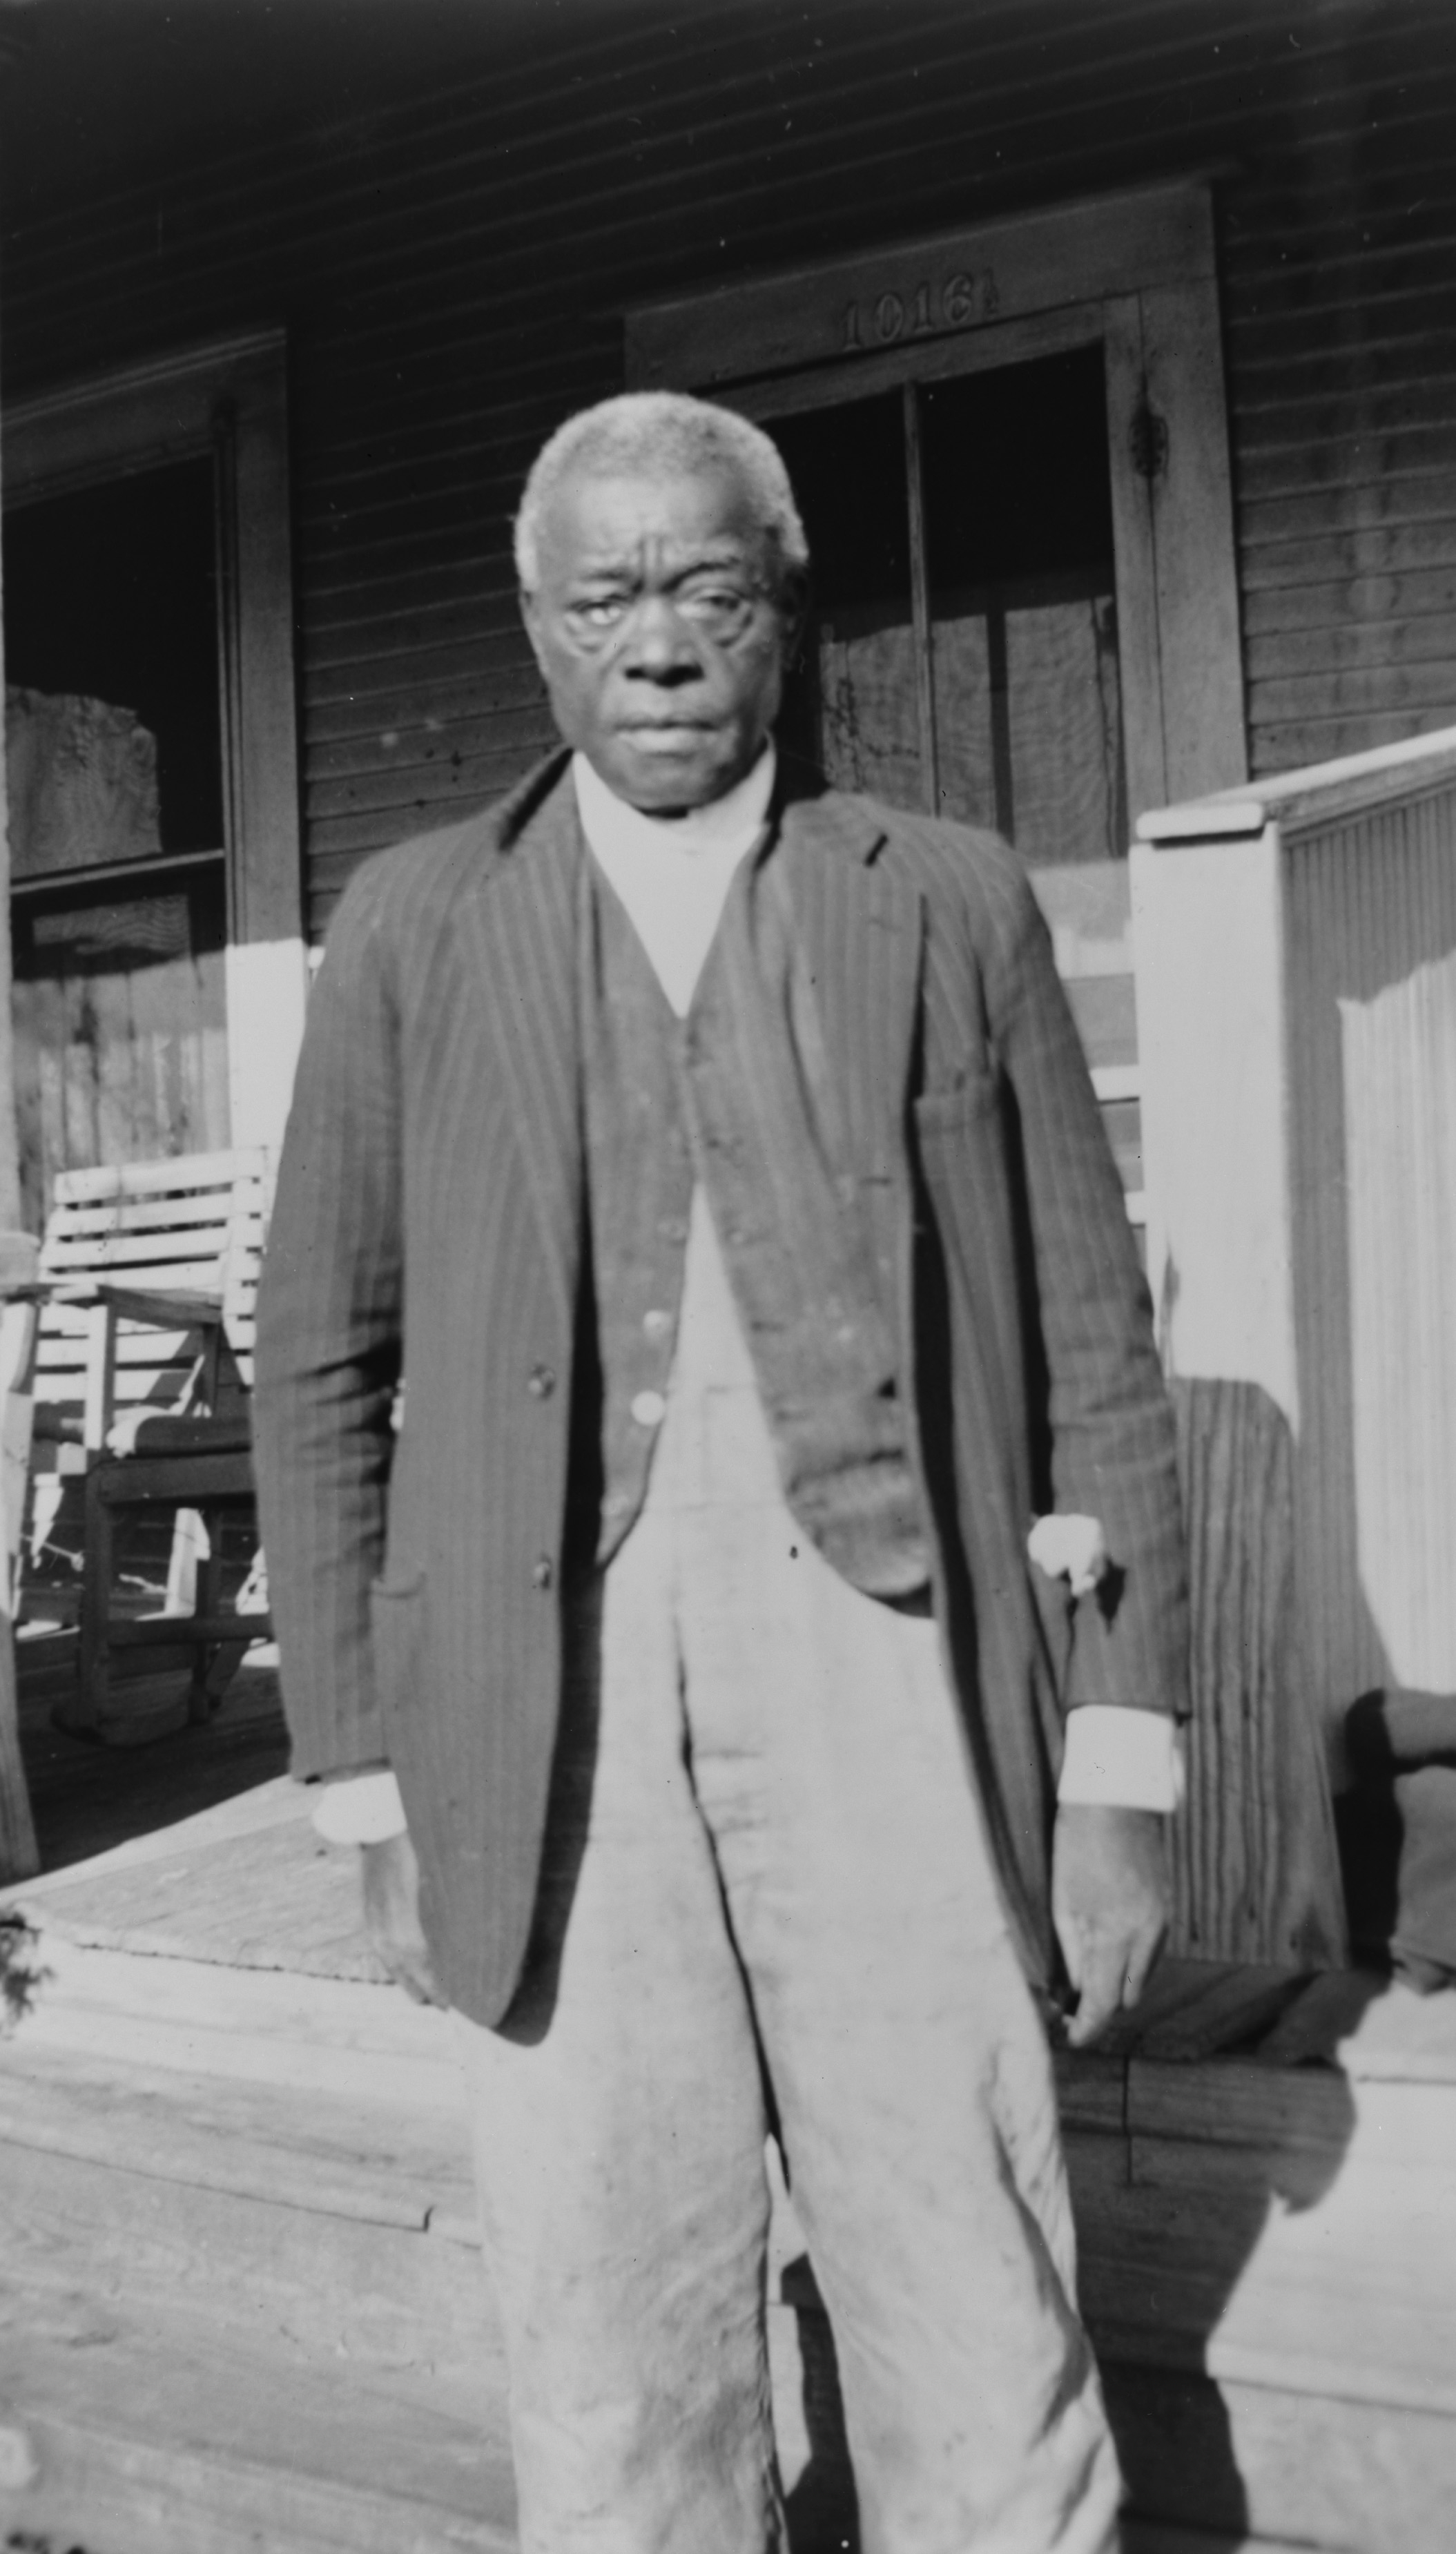
\includegraphics[width=90mm]{./imgs/williammoore_recorte.jpg} \label{img19}
\caption{William Moore}
%\end{minipage}
\end{figure}

\subsection{Cato Carter, narrativas do Texas, Parte~I,~página~203} \label{ref53}

``Algumas fazendas quase matavam os seus negros de fome e racionavam a
comida até eles não prestarem mais para trabalhar. Eles tinham que ir
escondido atrás dos negros nas outras fazendas para arranjar o que
comer. Eles tinham chamados no campo, e outros tipos de gritos e berros
com significados especiais''.

\paragraph{Comentário}\quad
{\small
A violência que ocorria era prova da crueldade opressora da
escravidão. Quando
chegavam ao seu limite e não podiam mais suportar maus"-tratos ou
injustiças, os cativos reagiam até isoladamente com violência. Muitas vezes, a violência irrompia porque saíam em defesa de um familiar. O Sul pré"-guerra era uma região
bastante violenta, mas dada a determinação da comunidade branca de
reprimir qualquer demonstração séria de resistência escrava, é incrível que os cativos tenham recorrido à violência tanto quanto o fizeram.
}

\subsection{William Moore, narrativas do Texas, Parte~\versal{III},~páginas~133--37}
\label{ref198}

``O senhor Tom está morto há muitos anos. Creio que está no inferno.
Acho que é o lugar dele. Era um homem terrível de mau, com uma mulher
antipática. Mas ele teve os melhores, mais gentis filhos que o Senhor
jamais deixou viver e respirar nesta terra. Eles eram tão bondosos,
tinham tanta pena de nós escravos. (\ldots{})

Um dia, eu estava no chiqueiro quando escutei um grito de agonia
horrível vindo da casa. Quando cheguei mais perto, vi que o senhor Tom
tinha amarrado mamãe a uma árvore e arrancado as roupas dela e agora
estava descendo o relho, com o sangue correndo pelos olhos e as costas
dela. Fiquei maluco. `Para, senhor Tom', eu disse, e ele virou o chicote
em mim. Não me acertou bem, mas me cortou igual. Vi a senhora Mary
parada na porta da cozinha, então corri feito louco e vi uma pedra bem
grande, que peguei e atirei no senhor Tom. Eu acertei na cabeça e ele
caiu feito um boi macetado. A senhora Mary veio, levantou o pai e levou
ele para dentro de casa, depois saiu e me ajudou a desatar mamãe. Mamãe
e eu nos escondemos no mato dois, três meses, acho. Minhas irmãs nos
encontravam para trazer mantimentos e passar graxa nas costas de mamãe.
Logo, logo elas disseram que seria seguro voltar para a choupana para
comer à noite e ficavam de olho no senhor Tom.

Um dia, a mulher do senhor Tom estava no pátio e me chamou, dizendo que
tinha alguma coisa para mim. Ela estava com a mão embaixo do avental,
pedindo para eu ir até ela. `Me dá a sua mão', ela disse. Eu estiquei
minha mão, que ela agarrou e passou uma corda com nó corrediço. Eu vi
que era isso que ela tinha embaixo do avental, com a outra ponta
amarrada em um arbustozinho. Tentei me soltar e sair correndo, fiz ela
tropeçar e cair, então ela quebrou o braço. Tirei a corda do braço e
fugi.

Mamãe e eu ficamos escondidos no mato depois disso. Vimos Sam e Billie e
eles nos contaram que estava brigando por causa dos negros. Depois eles
nos contaram que os negros declararam para o senhor Tom que as surras
tinham que terminar e que a gente poderia voltar e ficar na nossa
choupana, que eles iam garantir que o senhor Tom não ia fazer mais nada.
E foi isso que mamãe e eu fizemos. Sam e Billie eram os dois maiores
negros da fazenda, e eles deram um jeito de tirar as espingardas da
casa. Um dia, o senhor Tom estava na cadeira de balanço na varanda e Sam
e Billie estavam com a arma. Todos vimos cinco brancos chegarem a
cavalo. Quando chegaram perto, Sam disse para o senhor Tom: `O primeiro
branco que passar pela cerca leva um tiro'. O senhor Tom abanou para os
brancos recuarem, mas eles foram galopando até a cerca e saltaram dos
cavalos.

`Fiquem no lado de fora, por favor, cavalheiros, eu mudei de ideia', o
senhor Tom disse. `O que é que houve aqui? Viemos surrar os negros, foi
o que você nos contratou para fazer', eles disseram. `Pois mudei de
ideia, mas se ficarem aí no lado de fora eu lhes levo o dinheiro', o
senhor Tom disse.

Eles ficaram discutindo que queriam entrar, mas o senhor Tom convenceu
eles a não entrar, então eles disseram que iriam se ele lhes trouxesse
seus três dólares cada. Ele levou o dinheiro e eles foram embora.

O senhor Tom praguejou e gritou, mas os negros ficaram no mato, matando
tempo. Eles diziam que não adiantava trabalhar por nada todos os dias''.
{[}Após a emancipação, eles foram para o lar de um dos filhos do
senhor.{]}

\subsection{Fanny Moore, narrativas da Carolina do Norte, Parte~\versal{II},~páginas~132--33}
\label{ref195}

``Lembro que uma vez teve um baile em uma das casas da senzala. Todos os
negros estavam lá, rindo e sapateando e cantando, mas alguns não. Os
patrulheiros arrombaram a porta e começaram a nos agarrar. O filho do
Tio Joe decidiu que era hora de alguém morrer e começou a brigar. Ele
disse que estava cansado de aguentar tantas surras, que não aguentava
mais. Os patrulheiros começaram a bater nele e ele foi revidando. Ah,
meu Deus, foi um problema. Surraram ele com um chicote de couro por um
tempão, depois um deles pegou um pau e bateu na cabeça dele, a cabeça se
abriu toda. O coitado do menino caiu no chão, gemendo. Os patrulheiros
açoitaram mais outra meia dúzia de negros e mandaram eles embora e nos
deixaram com o menino morto''.

\subsection{Minnie Fulkes, narrativas da Virgínia, páginas 11--12} \label{ref96}

``E ela {[}sua mãe{]} disse que eles costumavam fazer cultos e cantar e
rezar, e que os velhos patrulheiros escutavam, então para não deixar o
som ir longe, os escravos colocavam um panelão de ferro enorme na porta.
Mas às vezes eles esqueciam de colocar a panela e os patrulheiros
chegavam e açoitavam todo mundo, sem esquecer ninguém, só porque as
pobres almas estavam rezando para Deus libertá"-los daquele cativeiro
horrível.

Rá, rá, rá! Tinha esse irmão que estava estudando com eles um dia e que
contou para todos os escravos como se vingar. Ele disse para amarrarem
parreiras e outras trepadeiras na estrada, então quando os patrulheiros
viessem galopando os cavalos iam estar correndo tão rápido que as
videiras iam se emaranhar com eles, e isso ia fazer os cavalos
tropeçarem e caírem. E várias vezes, eles caíam tão feio que quebravam
as pernas, e as dos cavalos também. Uma vez, um pobre diabo se emaranhou
bem e o cavalo seguiu em frente até ele cair do cavalo. No dia seguinte,
um coitado foi achado na estrada com as trepadeiras enroladas no
pescoço, tantas voltas que tinha se estrangulado, é o que dizem. Estava
totalmente morto. Bem feito, porque aqueles brancos nos tratavam muito
mal.

Ora, às vezes, pois é o que faziam, os outros seguiam até descobrir onde
estava acontecendo a reunião. Eles entravam e começavam a açoitar e a
bater nos escravos sem dó nem piedade. Tudo isso para não deixar eles
servirem a Deus, e saiba que alguns daqueles diabos eram pecadores e
malvados o suficiente para dizer isso mesmo. `Se eu pegar vocês servindo
a Deus, vão apanhar. Vocês não têm tempo para servir a Deus. Compramos
vocês foi para servir a nós'. Arrã. (\ldots{})

Sabe, os escravos eram espancados e maltratados; alguns tinham começado
a se juntar e matado os brancos quando levavam eles para o eito para
trabalhar. Deus está castigando aqueles diabos velhos e os filhos deles
agora mesmo pelo jeito que tratavam os pobres coitados dos negros''.

\begin{figure}[]
\centering
 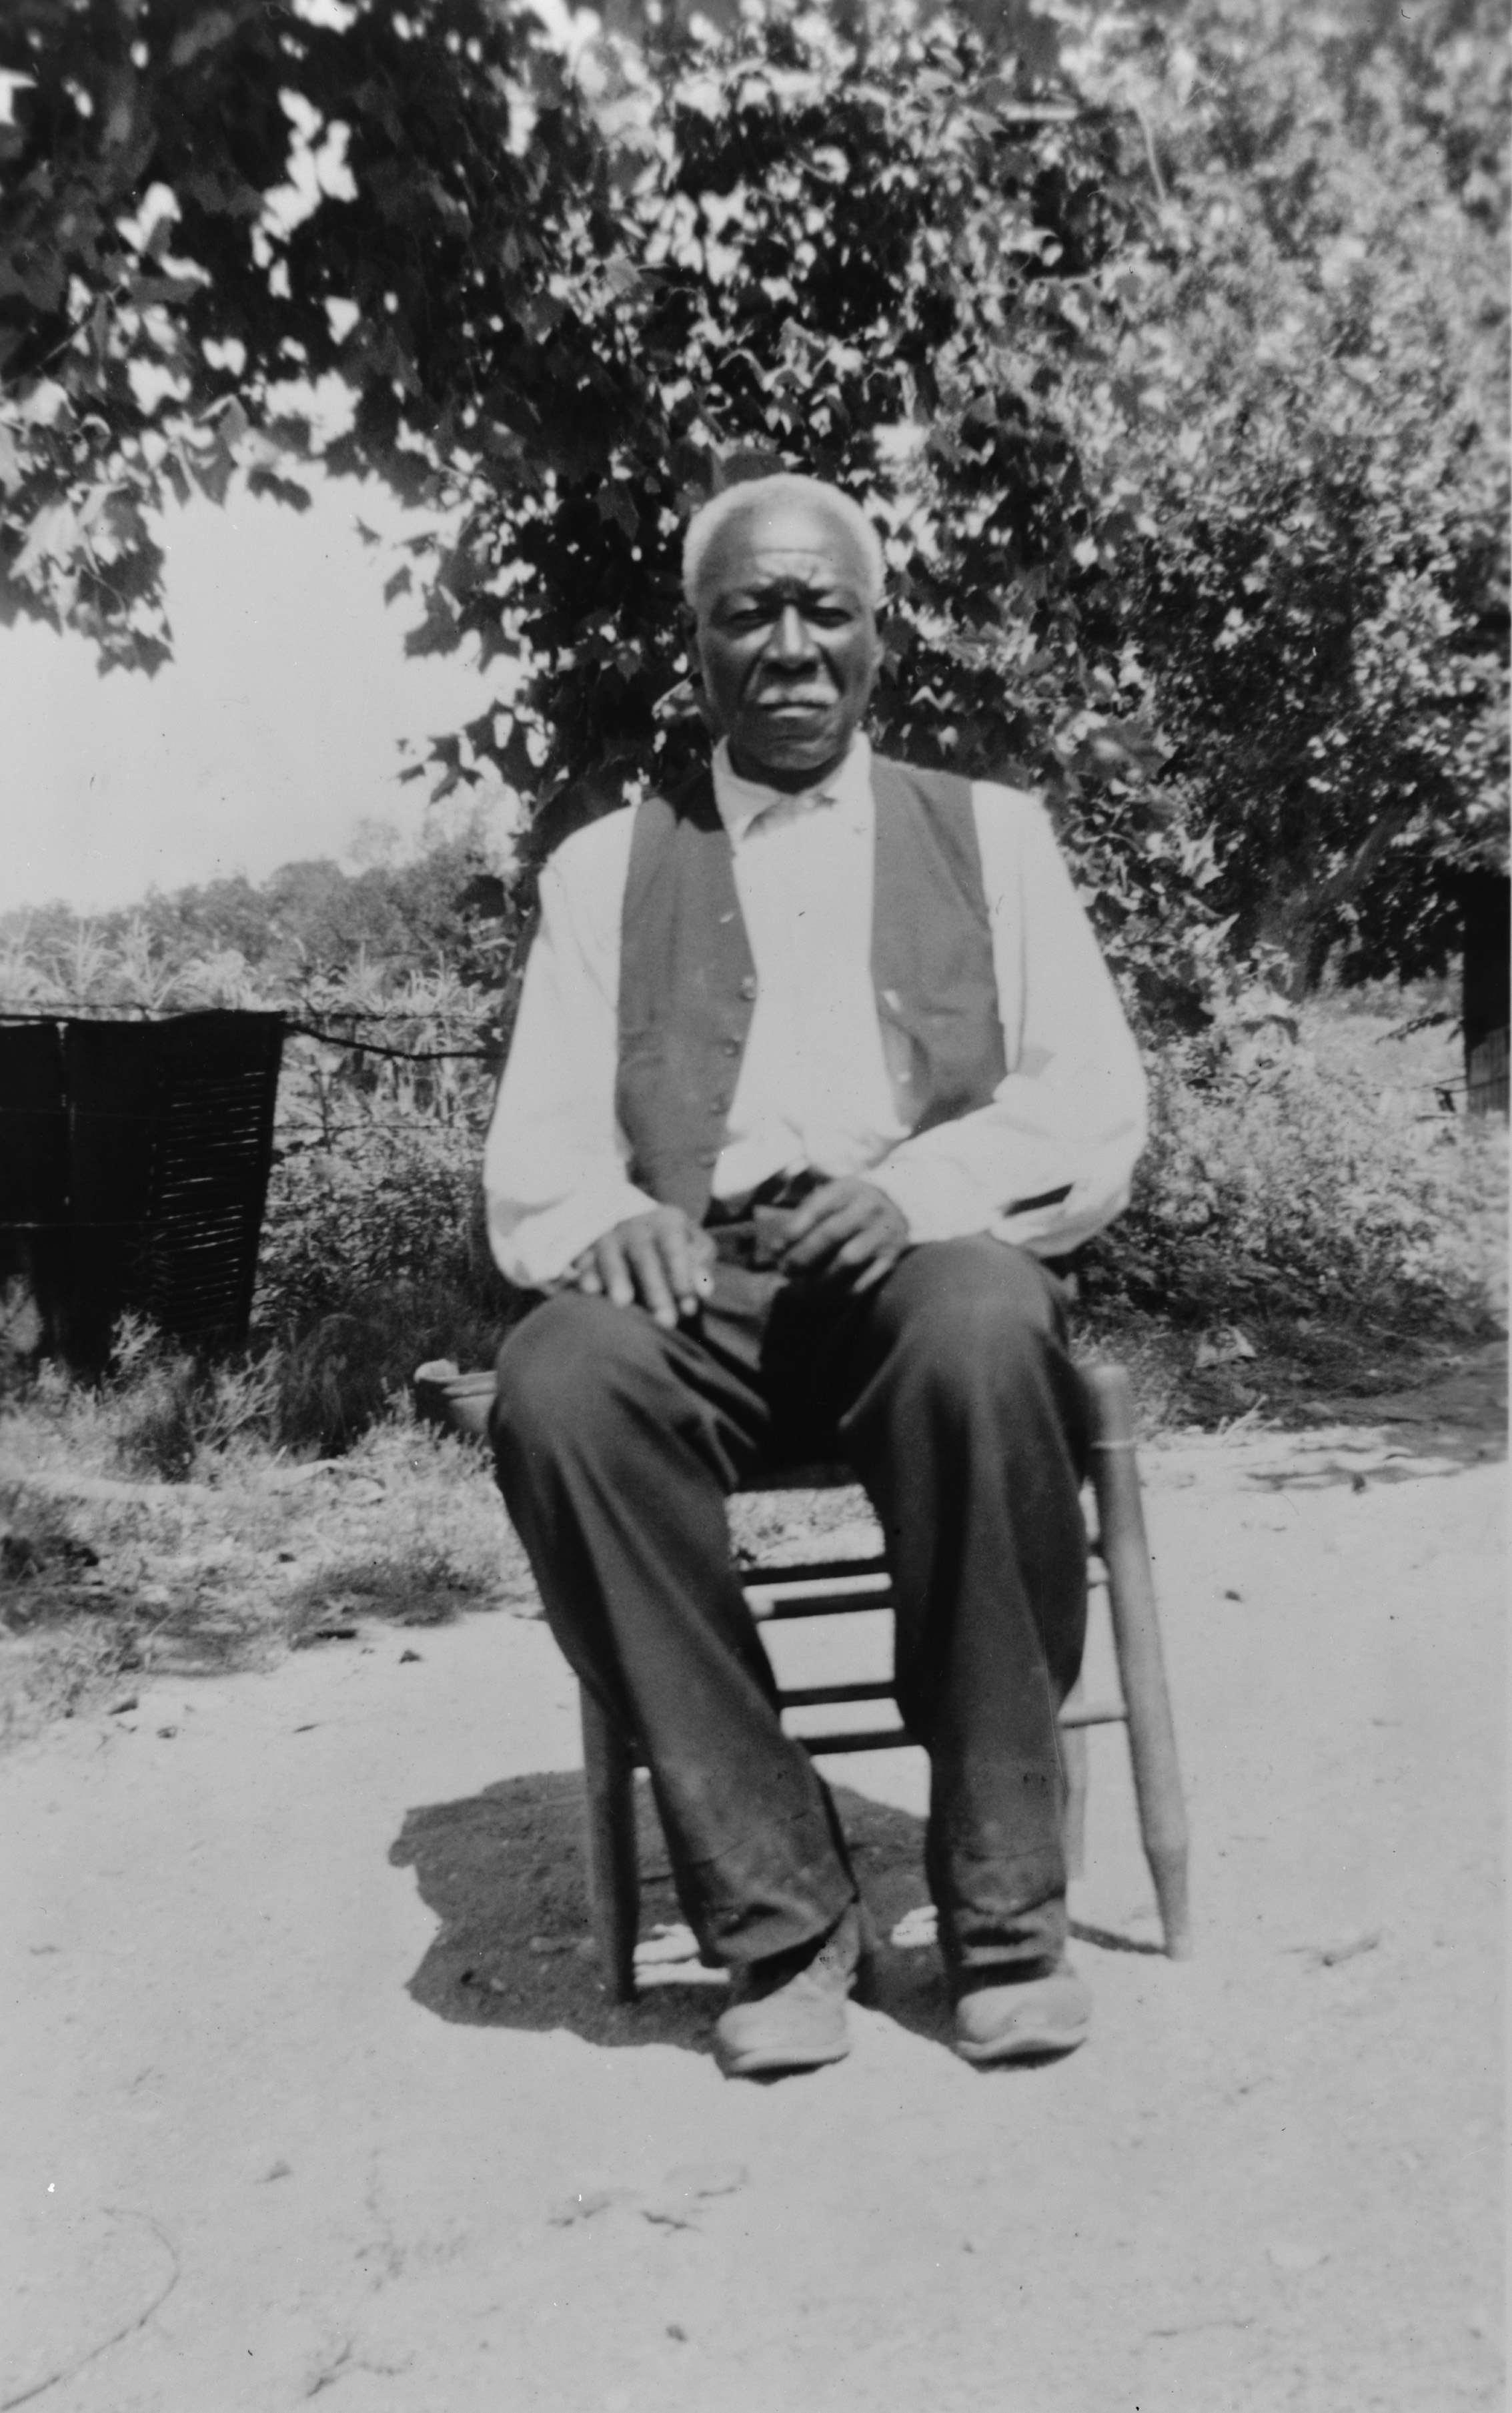
\includegraphics[width=90mm]{./imgs/williewilliams_recorte.jpg} \label{img20}
\caption{Willie Williams}
\end{figure}

\subsection{Sol Walton, narrativas do Texas, Parte~\versal{IV},~página~129}
\label{ref276}

``O senhor só teve um feitor branco, que morreu em uma briga. Os
escravos estavam queimando toras e lixo e o feitor derrubou um velho e
fez alguns dos outros negros segurarem ele enquanto era açoitado. O
velho se levantou e acertou o feitor na cabeça com um pedaço de pau,
então pegou um machado e cortou os pés e as mãos dele fora. O senhor
disse que não queria nunca mais ter um feitor branco, então meu primo
virou capataz depois disso''.

\subsection{Willie Williams, narrativas do Texas, Parte~\versal{IV},~página~188}
\label{ref294}

``Uma vez, os negros engambelaram os patrulheiros. Nesse baile, alguns
dos negros não tinham passes, e os patrulheiros estavam vindo. Os negros
decidiram dar uma lição neles, então alguém pegou uma panela de cinzas
quentes e, quando os patrulheiros entraram pela porta, as cinzas voaram
nas caras deles. Os negros saíram correndo e derrubaram os patrulheiros,
então sumiram. Foi uma vez que os negros surpreenderam os
patrulheiros''.

\subsection{George Womble, narrativas da Geórgia, Parte~\versal{IV},~página~182}
\label{ref311}

``Os escravos sabiam que sempre que o Sr. Womble contratava um novo
feitor, ele informava o candidato que se não pudesse lidar com os
escravos, seus serviços não seriam necessários. A cozinheira ouviu o
senhor dizer isso a um possível feitor, então sempre que um novo era
contratado, os escravos tentavam ver até onde podiam ir com ele. O Sr.
Womble diz que o feitor precisava ser muito competente para manter seu
emprego na fazenda dos Womble, pois se descobriam que ele tinha medo que
brigassem com ele (o que faziam, de tempos em tempos), os escravos
tiravam tanta vantagem dele que a produção decaía e o feitor era forçado
a prestar explicações ao seu empregador ou então a procurar um novo
emprego. O senhor nunca castigava um escravo por atacar um feitor usando
seus punhos, afirmou o Sr. Womble''.

\subsection{Ellen Cragin, narrativas do Arkansas, Parte~\versal{II},~página~42} \label{ref59}

``Ela {[}minha mãe{]} não trabalhava no eito. Ela trabalhava no tear,
por tanto tempo e tantas vezes que uma vez pegou no sono no tear. O
filho do senhor viu e contou para a mãe. A mãe mandou ele pegar um
chicote e lhe dar uma lição. Ele pegou um pedaço de pau e foi acordá"-la
a pancadas. Ele bateu na minha mãe até ela acordar. Quando acordou, ela
puxou uma vara do tear e bateu nele de volta até quase matá"-lo. `Não me
bate mais, eu não vou deixar eles açoitarem você', ele gritava. E ela
respondeu: `Eu vou te matar. Mamou nessas tetas negras e agora vem aqui
bater em mim'. E quando ela saiu, ele não conseguia mais caminhar.

E foi a última vez que a vi até após a liberdade. Ela saiu e subiu em
uma vaca velha que costumava ordenhar. Dolly, era assim que chamava. Ela
foi"-se embora da fazenda, porque sabia que iriam matá"-la se ficasse''.

\subsection{Campbell Armstrong, narrativas do Arkansas, Parte~I,~página~70} \label{ref12}

``Uma noite, eu estava em um baile. Tinha madeira de cerca na lareira. O
patrulheiro bateu à porta, entrou e fechou ela atrás de si. Um negro
puxou um pau da lareira e acertou no patrulheiro, então o patrulheiro
deu licença e deixou o negro passar. Os negros costumavam atravessar
cordas na estrada para fazer os cavalos dos patrulheiros tropeçarem''.

\subsection{Thomas Lewis, narrativas do Indiana, página 126}
\label{ref178}

``Não existia isso de ser bom para os escravos. Muitas pessoas eram
melhores do que as outras, mas o escravo pertencia ao seu senhor e não
havia como fugir disso. Era difícil fazer um homem forte trabalhar. Ele
brigava tanto que os brancos tentando segurá"-lo ficavam sem fôlego. Aí
não havia o que fazer além de matá"-lo. Se um escravo resistia e o seu
senhor o matava, era o mesmo que autodefesa hoje em dia. Se um senhor
cruel açoitava um escravo até a morte, isso amedrontava os outros
escravos''.

\subsection{Isaam Morgan, narrativas do Alabama, página 283}
\label{ref201}

``Nenhum dos nossos escravos jamais tentou fugir. Todos sabiam que
estavam bem de vida. A gente só teve feitor uma vez. Um homem malvado.
Ele tentou brigar e bater nos escravos, mas uma noite seis negros bem
grandes se juntaram e quase mataram ele de susto. Depois disso, o senhor
nunca mais quis ter feitores. Ele mesmo cuidava disso''.

\subsection{Susan Hamilton, narrativas da Carolina do Sul, Parte~\versal{II},~página~234}
\label{ref121}

``Nunca esqueço de Clory, a lavadeira. Ela era muito esquentada. Era uma
mulata com um cabelo lindo, tão grande que podia sentar nele. Clory não
aceitava besteira de ninguém. Um dia, nossa senhora foi à lavanderia e
encontrou defeitos nas roupas. Clory não fez nada, só pegou a senhora e
atirou ela porta afora. Tiveram que chamar um doutor, porque ela estava
grávida e o bebê nasceu menos de duas horas depois. Depois disso ela
implorou para ser vendida, porque não {[}queria{]} matar a senhora, mas
nosso senhor nunca queria vender os seus escravos. Mas isso não impediu
Clory de ser açoitada, e foi brutal. Açoitaram até não sobrar um pedaço
branco que fosse no corpo dela. Foi o pior que já vi um ser humano ser
surrado. Achei que ela ia morrer, mas ela melhorou e não se adoçou nada,
só ficou mais braba até o nosso senhor decidir que era melhor alugá"-la.
Ela concordou na mesma hora, porque assim não ficava por perto da
senhora. Ela odiava e detestava os dois e toda a família''.

\subsection{Sra. Josie Jordan, narrativas do Oklahoma, páginas 160--61}
\label{ref165}

``Salina era o nome da minha mãe, e ela pertenciam a um tal Sr. Clark,
que vendeu ela e papai para Mark Lowery porque ela era uma mulher
brigona e cabeçuda.

Não era culpa dela, ser de briga. O senhor que era dono dela antes do
Sr. Clark era um desses brancos que estão sempre açoitando e batendo nos
seus escravos, e mamãe não aguentava mais.

Foi assim que ela me contou. Ela decidiu que era melhor morrer e acabar
com essa desgraça do que ser açoitada o tempo inteiro, então um dia o
senhor disse que havia algo de errado com o trabalho e foi erguer o
chicote, mas mamãe revidou. Quando a confusão terminou, o senhor estava
caído no chão, tão parado que acharam que ele estava morto, de tanto que
apanhou.

Mamãe diz que ele não morreu, e que logo depois ela foi vendida para
esse Sr. Clark de que eu estava lhe falando. E mamãe sofreu uma miséria
por muito tempo depois de ser levada para a fazenda de Mark Lowery, onde
eu nasci durante a guerra''.

\paragraph{Comentário}\quad
{\small
Uma opção para os escravizados era fugir. Alguns conseguiam
escapar para os estados livres ou para o Canadá. Estima"-se que 100 mil
podem ter conquistado sua liberdade dessa maneira durante todo o período
pré"-guerra, e até 1000 por ano na década de 1850, apesar de o Congresso
ter aprovado a Lei do Escravo Fugitivo em 1850, que dificultava a
prática. Mas as fugas eram arriscadas, mesmo para os que
começavam a jornada em um dos estados que faziam fronteira com os
estados livres do Norte. Havia uma rede informal de negros e brancos
simpatizantes, chamada de ``Ferrovia Subterrânea'', que era útil, mas a
maior parte do esforço e dos riscos dependiam da iniciativa individual.
Aqueles em cativeiro mais ao Sul tinham uma distância muito maior a
percorrer, através de territórios nos quais todos os brancos estavam
alertas e eram hostis, de modo que a fuga era praticamente impossível.

As Narrativas de Escravos do \versal{FWP} revelam que era muito mais comum
fugir para a floresta, ausentando"-se da fazenda e se
escondendo nos arredores. Lá, eles escapavam da vigilância fácil
possibilitada pelo terreno desmatado das fazendas, e podiam caçar,
procurar abrigo e se deslocar para não ser pegos. Ao fugir para a
floresta, muitos começavam um processo de barganha com os seus
proprietários. O senhor queria e precisava da mão de obra escrava, então
sua ``propriedade'' não rendia quando não estava presente. Às
vezes, o escravizado conseguia, através de intermediários, acertar o seu
retorno após a solução de alguma queixa ou mudanças no tratamento dado.
Isso nem sempre tinha êxito, mas fica evidente que os senhores de
escravos tinham muita dificuldade para capturar quem se escondia, mesmo
quando usavam cães de caça para procurar os fugitivos.
}

\subsection{Annie Huff, narrativas da Geórgia, Parte~\versal{II},~páginas~235--36}
\label{ref150}

``Aquele que buscavam escapar de um senhor cruel costumavam esfregar
terebintina nas solas dos pés para impedir sua captura. Outros coletavam
quantidades de solo de um cemitério e o polvilhavam sobre seus rastros
até uma determinada distância. Ambas as precauções eram usadas para
desviar os cães farejadores. Os escravos refugiados muitas vezes se
abrigavam nas terras do Sr. Huff, onde eram auxiliados pelos negros da
família Huff na parte subsequente da fuga. Aqueles que permaneciam na
floresta eram alimentados regularmente. (\ldots{}) Os escravos
comemoravam todas as notícias, por menores que fossem, que recebiam
sobre a probabilidade de serem libertados pelos yankees''.

\subsection{Gus Smith, narrativas do Missouri, página 332}
\label{ref243}

``Nabo selvagem cresce aos milhares nos matos daqui. Uns campos cheios,
parecem nabos, crescem às pencas, bem vermelhos. Os negros usavam nabo
selvagem nos tempos da escravidão. Eles colhiam, secavam, pulverizavam e
amarravam em quantidade ao redor dos pés para os cães de caça não
pegarem o rastro. Cão nenhum ia longe depois de sentir o cheiro. É forte
feito pimenta vermelha e queima feito nada, os negros sempre usavam para
fugir''.

\subsection{Charles Crawley, narrativas da Virgínia, página 8} \label{ref62}

``Quando os escravos fugiam, eles eram levados de volta para os seus
senhores e senhoras; quando não conseguiam pegá"-los de volta, eles
deixavam isso para lá. Às vezes, os escravos saíam e iam morar em outros
lugares; alguns moravam no mato, vivendo do que roubavam: porcos, milho
e verduras das fazendas dos outros''.

\subsection{Elisabeth Sparks, narrativas da Virgínia, página 51}
\label{ref251} 

``Bater em mulheres? Mas claro que batia em mulheres. Batia nas
mulheres igual batia nos homens. Batia nas mulheres peladas e lavava com
salmoura. Às vezes, batia tanto que elas não se aguentavam e fugiam para
o mato. Se você entrava no mato, eles não tinham como te pegar. Podia
se esconder, e as pessoas traziam de comer para você. Então ele chamava
por você todos os dias. Depois de um tempo, ele dizia para um dos
capatazes negros dizer para você voltar. Não vai mais bater em você.
Eles tinham um capataz negro, mas sempre com um feitor branco. O capataz
a convencia a voltar e então ele matava você a pancadas de novo''.

\subsection{Henry Wright, narrativas da Geórgia, Parte~\versal{IV},~página~202}
\label{ref321}

``Sempre que um escravo tentava fugir, colocavam os cães para
rastreá"-los. O Sr. Wright foi pego e encurralado pelos cães diversas
vezes, mas posteriormente descobriu uma maneira de evadi"-los. Para
tanto, ele esfregava nos pés os dejetos do quintal ou do pasto e então
cobria as pernas com alcatrão de pinheiro. Em uma ocasião, ele conseguiu
manter"-se seis meses afastado da fazenda antes de voltar por conta
própria. Ele fugiu após atacar seu senhor, que tentara açoitá"-lo. Quando
voltou por conta própria, o senhor não fez nada, pois ficou contente em
saber que ele não se perdera para sempre, o que levaria à perda de uma
soma considerável. (\ldots{}) Quando fugitivo, ele dormiu na floresta,
comeu frutas silvestres, etc. Às vezes, ele fugia para a fazenda da sua
mãe ou a do seu pai, onde conseguia obter alimentos''.

\subsection{Essex Henry, narrativas da Carolina do Norte, Parte~I,~página~397}
\label{ref138}

``Tinha um homem em Raleigh com dois cães de caça que ganhava a vida
caçando negros fujões. O nome dele era Beaver, nunca deixava ninguém
escapar, exceto uma vez. Pat Norwood levou uma foice bem comprida quando
fugiu, e quando o primeiro cão apareceu ele cortou o rabo dele fora, do
segundo ele cortou a orelha, e os cachorros pararam de correr atrás
dele''.

\subsection{Jefferson Franklin Henry, narrativas da Geórgia, Parte~\versal{II},~páginas~185,~187}
\label{ref140}

``Teve um escravo em quem ele nunca encostou. (\ldots{}) Aquele
encarregado dele, Robert Scott, fugiu e ficou fora uns dias uma vez. O
senhor Robert tinha começado a açoitar a esposa dele, então ele pulou
entre os dois. Isso deixou o senhor Robert tão brabo que correu para
casa para buscar a arma, então o encarregado sumiu de vista um dia ou
dois para não levar tiro. Quando voltou, o senhor Robert ficou tão
contente em ter ele de volta que nunca disse uma palavra para ele sobre
ter ido embora''.

\subsection{Leah Garrett, narrativas da Geórgia, Parte~\versal{II},~página~14} \label{ref102}

``Um dos escravos se casou com uma menina e botaram ela para trabalhar
na casa grande. Um dia, a senhora atacou ela por causa de alguma coisa e
a menina revidou. A senhora disse que ia pedir para o senhor colocá"-la no
tronco e bater nela quando chegasse em casa. Quando a menina foi para o
eito e contou para o marido, ele disse aonde ela deveria ir e para ficar
lá até ele chegar. Naquela noite, ele levou a própria janta para ela,
depois levou a menina até uma caverna, carregou uma palha e arrumou tudo
para ela dormir. Ele arrumou aquela caverna como se fosse uma casa,
colocou um fogão e correu um cano pela terra até um pântano. Todo mundo
sempre se perguntou como ele arrumou aquele cano, mas é claro que eles
não cozinhavam até de noite, quando ninguém ia enxergar a fumaça. Ele
fez um forro de toras de pinheiro, fez camas e mesas com troncos de
pinheiro. Eles moraram sete anos nessa caverna. Tiveram três filhos
nesse tempo. Ninguém estava com ela quando esses filhos nasceram, só o
marido. Ele cuidou dela com cada filho. As crianças não vestiam nada de
roupa, só um pano amarrado na cintura. Eles eram peludos e cabeludos
feito gente do mato, e é o que eram. Quando saíam daquela caverna, eles
fugiam sempre que enxergavam alguém.

Durante os sete anos que ela morou naquela caverna, várias pessoas
ajudaram eles a ter comida. O marido levava até um certo lugar e ela ia
buscar. Muita gente passou na frente dessa caverna, várias e várias
vezes, mas ninguém nunca soube que tinha gente morando lá. Nosso senhor
não sabia onde ela estava, e foi só depois da liberdade que ela saiu de
vez da caverna''.

\subsection{Martha Jackson, narrativas do Alabama, página 220}
\label{ref160}

``Então eles não deixavam ninguém ir a lugar nenhum, nem quando as duas
fazendas eram vizinhas encostadas. Buscavam eles de lá e surravam de
novo, e é exatamente por isso que vários e vários fugiram. Conheço um
negro que ficou fora quase um ano, e ele não tinha ido muito longe, só
subido a estrada um pouco. Ficou morando em uma caverna que escavou em
uma encosta de argila. E a senhora Betty disse: `Marty, onde você acha
que está o Dan?' E eu nunca disse nada. Os patrulheiros não achavam ele
nem ninguém, e ele nunca aparecia à luz do dia até aparecer depois da
rendição''.

\subsection{Harriet Robinson, narrativas do Oklahoma, página 272}
\label{ref227}

``Por falar em negros que fugiram, meu padrasto não fugiu? Meu tio Gabe
não fugiu? O gelo só comia os dedos dos pés deles enquanto estavam
fugidos. Jogaram Tio Isom (meu padrasto) na cadeia e, enquanto estava
lá, ele matou um guarda branco. Colocaram no jornal, `Um negro a matar',
e nosso senhor viu e comprou ele. Era um homem com a força de dois, de
tão forte que era. Quando fugia, Deus lhe acuda. Uma vez, botaram os
cachorros atrás dele, mas ele pegou o líder da matilha e bateu no resto
dos cachorros. Os brancos pegaram ele de surpresa e fizeram os cachorros
comerem a orelha dele todinha. Mas, você não sabe, ele ainda conseguiu
fugir. Uma manhã, eu estava varrendo a sala da casa grande e alguém
bateu à porta da frente, então fui atender. Lá estava Tio Isom, com a
cabeça cheia de farrapos. `Vai dizer para o velho senhor que eu voltei',
ele me disse. Bati à porta do senhor e disse: `Senhor coronel Sam, Tio
Isom disse que voltou'. `Vá até a cozinha e diz para a mãe negra lhe dar
café da manhã', ele me respondeu. Quando ele terminou de comer, deram
300 chibatadas nele. Deus me abençoe, ele foi e fugiu de novo''.

\subsection{Louisa Gause, narrativas da Carolina do Sul, Parte~\versal{II},~página~110}
\label{ref104}

``Às vezes, quando não queriam fazer o que mandavam, os negros se
escondiam no mato e ficavam lá até o feitor ir atrás deles. Ah, eles
achavam com os cachorros. Quando o feitor encontrava quem tinha fugido,
ele botava o cachorro a caçar. Meu Deus, minha filha, mas aqueles
cachorros sempre achavam. Às vezes, eles corriam até você escalar uma
árvore, mas outras eles pegavam onde não tinha árvore para escalar''.

\subsection{Easter Wells, narrativas do Oklahoma, página 317}
\label{ref281}

``Mamãe era a cozinheira. Lembro que o velho senhor tinha umas regras
bem estritas, e uma delas era que se queimava o pão, você tinha que
comê"-lo. Um dia, mamãe queimou o pão. Ela estava ocupada demais e
esqueceu e ele queimou feio. Ela sabia que o velho senhor ia ficar
furioso e que seria castigada, então arrebanhou um pouco de comida e o
seu toucado e saiu em disparada. Ela se escondeu no mato e nos canaviais
por duas semanas e ninguém achava ela. Uma das mulheres levava comida
para ela às escondidas. Finalmente, ela voltou para casa e o velho
senhor desceu a chibata, mas não machucou ela. Ele ficou feliz de ter
ela de volta. Ela nos contou que podia ter fugido para o Norte, mas não
queria deixar os filhos para trás. Ela tinha medo de o senhorzinho ficar
brabo e nos vender para uma vida difícil, então voltou''.

\paragraph{Comentário}\quad
{\small
Em comparação com os fugitivos, um número menor de entrevistados
descreveu ações que havia realizado durante a Guerra Civil para auxiliar
os exércitos do Norte. Esse número menor provavelmente se deve ao fato
de que a maioria dos entrevistados era relativamente jovem durante a
guerra. Contudo, não há dúvida nenhuma de que a população escrava do Sul
foi um ativo essencial para a causa da União. Os generais de ambos os
exércitos afirmaram que os escravizados ajudaram o Norte de inúmeras
maneiras, atuando como espiões, fornecendo informações locais valiosas
ou auxiliando prisioneiros da União fugitivos. Eles também foram
soldados e trabalhadores no exército da União.

Antes do verão de 1863, os exércitos do Norte haviam avançado
relativamente pouco no território sulista ao longo da costa do
Atlântico, do rio Mississippi e da fronteira norte da Confederação. Após
a queda de Vicksburg, Mississippi, em julho de 1863, no entanto, 
milhares de escravizados do Vale do Mississippi atravessaram as linhas da 
União. Os generais nortistas William Tecumseh Sherman e Ulysses S. Grant
começaram a planejar uma invasão mais profunda, atacando o interior do
estado da Geórgia. Essa invasão, a chamada ``Marcha ao Mar'' de Sherman,
ocorreu em 1864. No ano seguinte, seu exército avançou para o Norte,
através das Carolinas, enquanto Grant atacava a massa do exército
sulista na Virgínia. Essas ações levaram ao fim da guerra.

No total, aproximadamente 500 mil escravizados atravessaram as linhas
da União durante o conflito. As mulheres, homens idosos e crianças
moravam em acampamentos de ``contrabando'' ou em fazendas abandonadas,
trabalhando como fazendeiros ou trabalhadores braçais para ajudar o
Norte. Enquanto isso, dezenas de milhares de homens jovens se tornaram
soldados. A União se beneficiou enormemente dos 180 mil soldados negros,
que lutaram bravamente em muitas batalhas. A maioria desses homens era
oriunda da população escrava, de modo que estavam ao mesmo tempo
ajudando o Norte e negando ao Sul o acesso à sua mão de obra. Esses
libertos contribuíram em muito para dar ao Norte sua margem de vitória.
}

\subsection{Mingo White, narrativas do Alabama, páginas 417--18}
\label{ref288}

``Depois que o velho Ned levou uma surra tão terrível por rezar por
Liberdade, ele fugiu e foi para o Norte se juntar ao Exército da União.
Depois que entrou para o exército, ele escreveu para o senhor Tom. Na
carta, ele dizia `estou deitando, senhor, e acordando, senhor', querendo
dizer que ia para cama quando sentia vontade e levantava quando bem
entendia. Ele disse a Tom White que se o queria, ele estava no exército
e que poderia vir atrás dele. Depois que o velho Ned foi para o Norte,
os outros começaram a procurar uma chance para fugirem. Vários foram
pegos e trazidos de volta. Eles sabiam o preço que iam ter que pagar, e
isso fez com que alguns se desesperassem. Em vez de levar uma surra,
eles escolhiam revidar até conseguirem escapar ou então morrer antes
que levassem a surra''.

\subsection{Mary Barbour, narrativas da Carolina do Norte, Parte~I,~páginas~80--81} \label{ref15}

``A gente tinha medo dos yankees no começo, mas quanto mais pensava em
fugir dos nossos senhores, mais tinha medo dos rebeldes. Seja como for,
papai disse que a gente ia se juntar aos yankees.

Viajamos a noite inteira e nos escondemos no mato o dia inteiro por um
tempão, mas finalmente chegamos na fazenda do Dr. Billard, no Condado de
Chowan {[}na Carolina do Norte{]}, acho que ficamos lá por vários dias.

Os yankees tomaram essa fazenda então nós paramos por lá, nos divertimos 
à beça dançando e tudo mais até sairmos. Os yankees disseram a papai
para ir para New Bern {[}uma cidade litorânea ocupada pelo exército do 
Norte{]} e que lá cuidariam dele, então é para New Bern que fomos''. 

\pagebreak
\thispagestyle{empty}
\movetoevenpage
\thispagestyle{empty}

\begin{absolutelynopagebreak}
\begin{vplace}
\begin{figure}[H]
\begin{adjustwidth}{-1.6cm}{}
  %\centering
  \vspace*{-2cm}
  %\hspace{-0.5cm}
  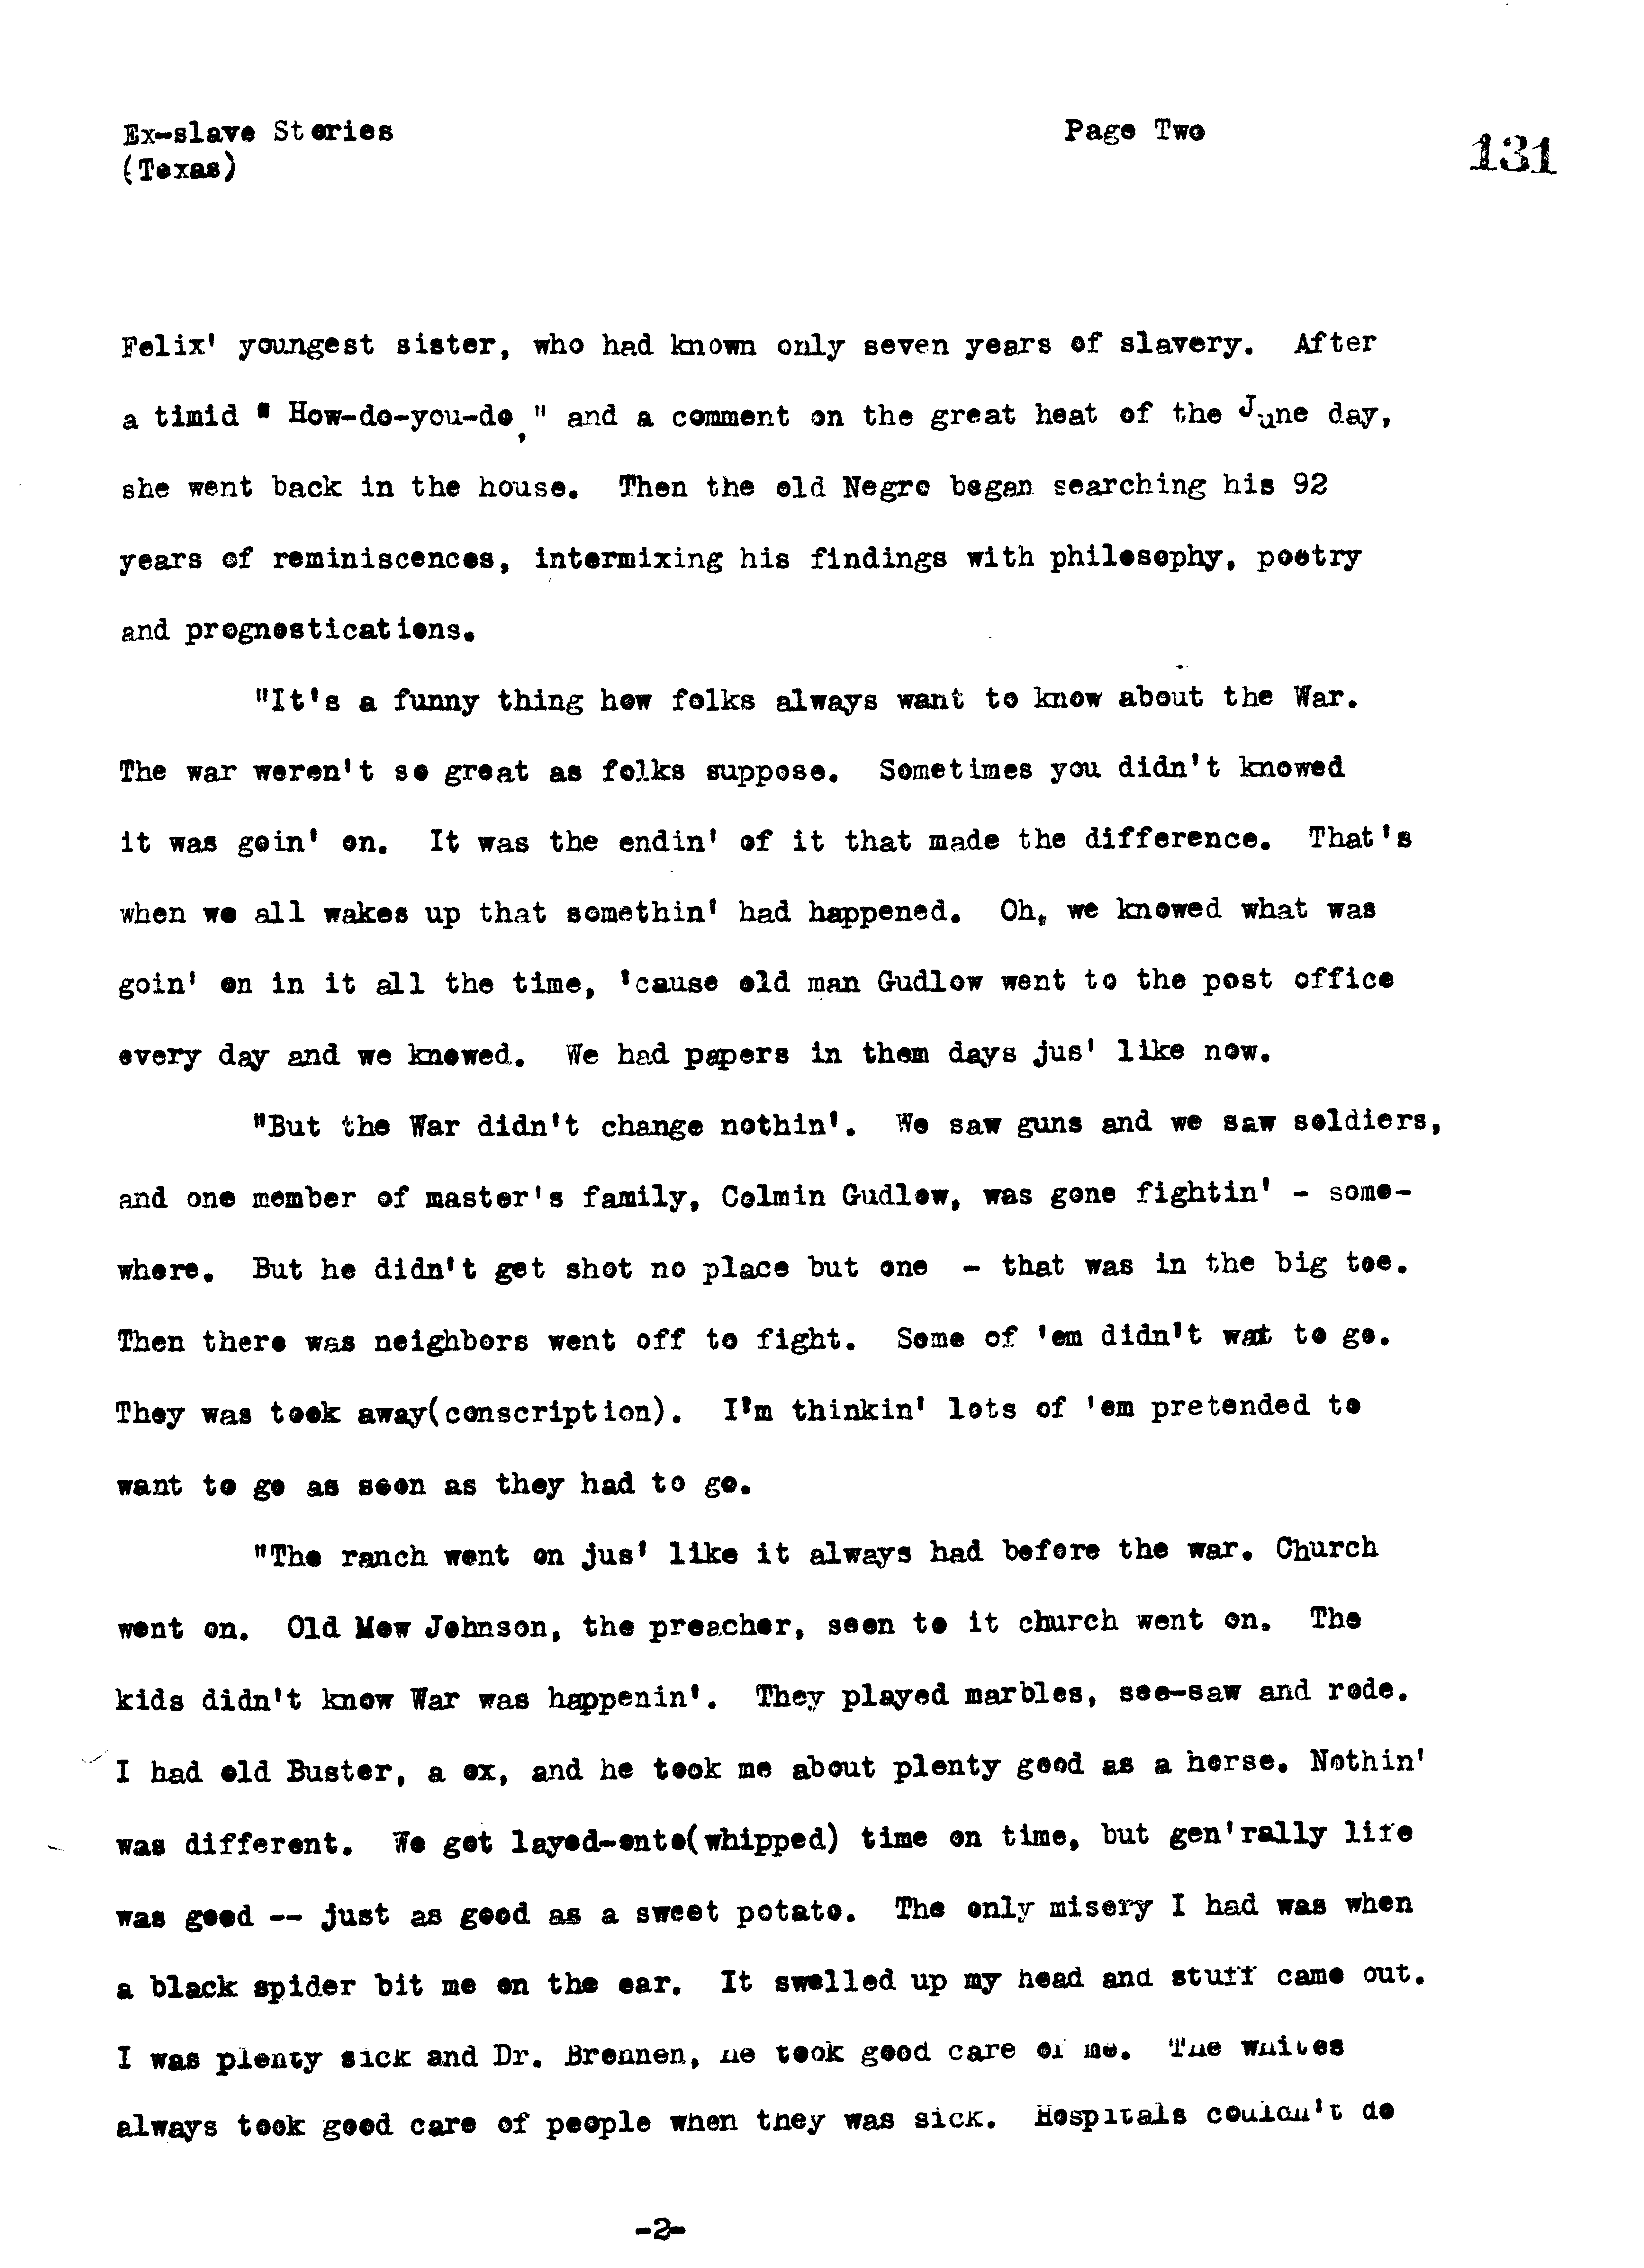
\includegraphics[width=130mm]{./imgs/Cap8.jpg}  
  %\hfill
\end{adjustwidth}
  \caption{Felix Haywood, narrativas do Texas, Parte \versal{II}, página 131}
\end{figure}
\end{vplace}

\end{absolutelynopagebreak}

\chapter*{Emancipação}
\addcontentsline{toc}{chapter}{Emancipação
\medskip}
\hedramarkboth{Emancipação}{}

\subsection{Felix Haywood, narrativas do Texas, Parte \versal{II}, página 131}
\label{ref134}

``É engraçado como todo mundo sempre quer saber da guerra. (\ldots{})
ah, a gente sempre sabia o que estava acontecendo, porque o velho Gudlow
ia até o correio todos os dias, então a gente sabia. Tinha jornal
naquele tempo, igual tem hoje. (\ldots{})

`Como vocês souberam que a guerra terminara?', perguntam os
entrevistadores.

Como a gente soube? Estourou um Aleluia:

\begin{verse}
Abe Lincoln freed the nigger\\
With the gun and the trigger\\
And I ain't goin' to get whipped any more\\
I got my ticket\\
Leavin' the thicket\\
And I'm a"-headin' for the Golden Shore.\footnotemark
\end{verse}

\footnotetext{Tradução: ``Abe Lincoln libertou os negros/ Com a arma e o gatilho/ E eu não vou mais ser
açoitado/ Ganhei meu bilhete/ Estou deixando o mato/ E partindo para a Costa
Dourada.''}

De repente, os soldados estavam por toda parte, chegando aos montes,
cruzando e caminhando e cavalgando. Todo mundo estava cantando,
caminhando em nuvens douradas. Aleluia!

\begin{verse}
Union forever\\
Hurrah, boys, hurrah\\ 
Although I may be poor\\ 
I'll never be a slave---\\ 
Shoutin' the battle cry of freedom.\footnotemark
\end{verse}

\footnotetext{Tradução: ``União para sempre/ Viva, rapazes, viva/ Eu posso ser pobre/ Mas nunca vou ser escravo/ Com o grito de guerra da liberdade.''}

Todo mundo foi à loucura. Nós nos sentíamos como os cavalos, e ninguém
nos deixara daquele jeito, só nós mesmos. Éramos livres. Simples assim,
éramos livres. Os brancos nem pareciam brabos. Eles continuaram a nos
dar comida, igual a antes. Ninguém tomou nossas casas, mas logo de
início os negros começaram a se mudar. Eles pareciam querer chegar mais
perto da liberdade, para saberem como ela era, como se fosse uma fazenda
ou uma cidade''.

\paragraph{Comentário}\quad
{\small
Como lembra Felix Haywood, a emancipação foi motivo para
rejubilação entre os escravizados. Uma minoria (talvez 500 mil de cerca de 4
milhões) conquistaram sua liberdade antes do fim da guerra,
quando os exércitos da União invadiram partes do Sul. Muitos
serviram ou trabalharam para o exército da União, mas muitos
dos seus familiares adoeceram ou morreram em acampamentos de
``contrabando'' mal aprovisionados. A maioria sabia que
estava livre após o fim da guerra, em abril de 1865, mas senhores de
escravos recalcitrantes chegaram a atrasar a emancipação em dois meses
em partes isoladas do Sul, até a chegada das tropas federais.

Durante quatro anos, os escravizados acompanharam o desenrolar da
guerra de perto. Na verdade, alguns brancos se espantavam ao descobrir
que os cativos muitas vezes sabiam sobre batalhas importantes antes de
essas informações chegarem aos seus senhores. Naturalmente, os escravizados
observavam seus senhores em busca de notícias sobre eventos e de
informações sobre as atitudes dos brancos. O modo como os proprietários
reagiam era um prenúncio das atitudes que teriam a respeito dos negros
depois do fim da escravidão.

Os negros do Sul descobriram que a possível derrota da
Confederação iria apenas enfurecer alguns dos brancos e os deixaria
ainda mais hostis à chegada da liberdade. Os brancos que tinham dinheiro
suficiente muitas vezes levavam suas escravarias para regiões que, eles
imaginavam, estariam seguras das tropas yankees, pois estavam decididos
a sustentar a escravidão. Outros aceitaram as mudanças da guerra, ainda
que a maioria o tenha feito com tristeza ou relutância. Relativamente
poucos senhores procuraram suas antigas ``propriedades'' com o espírito
de cooperação.
}

\begin{figure}[]
%\begin{minipage}{0,4\textwidth}
\centering
 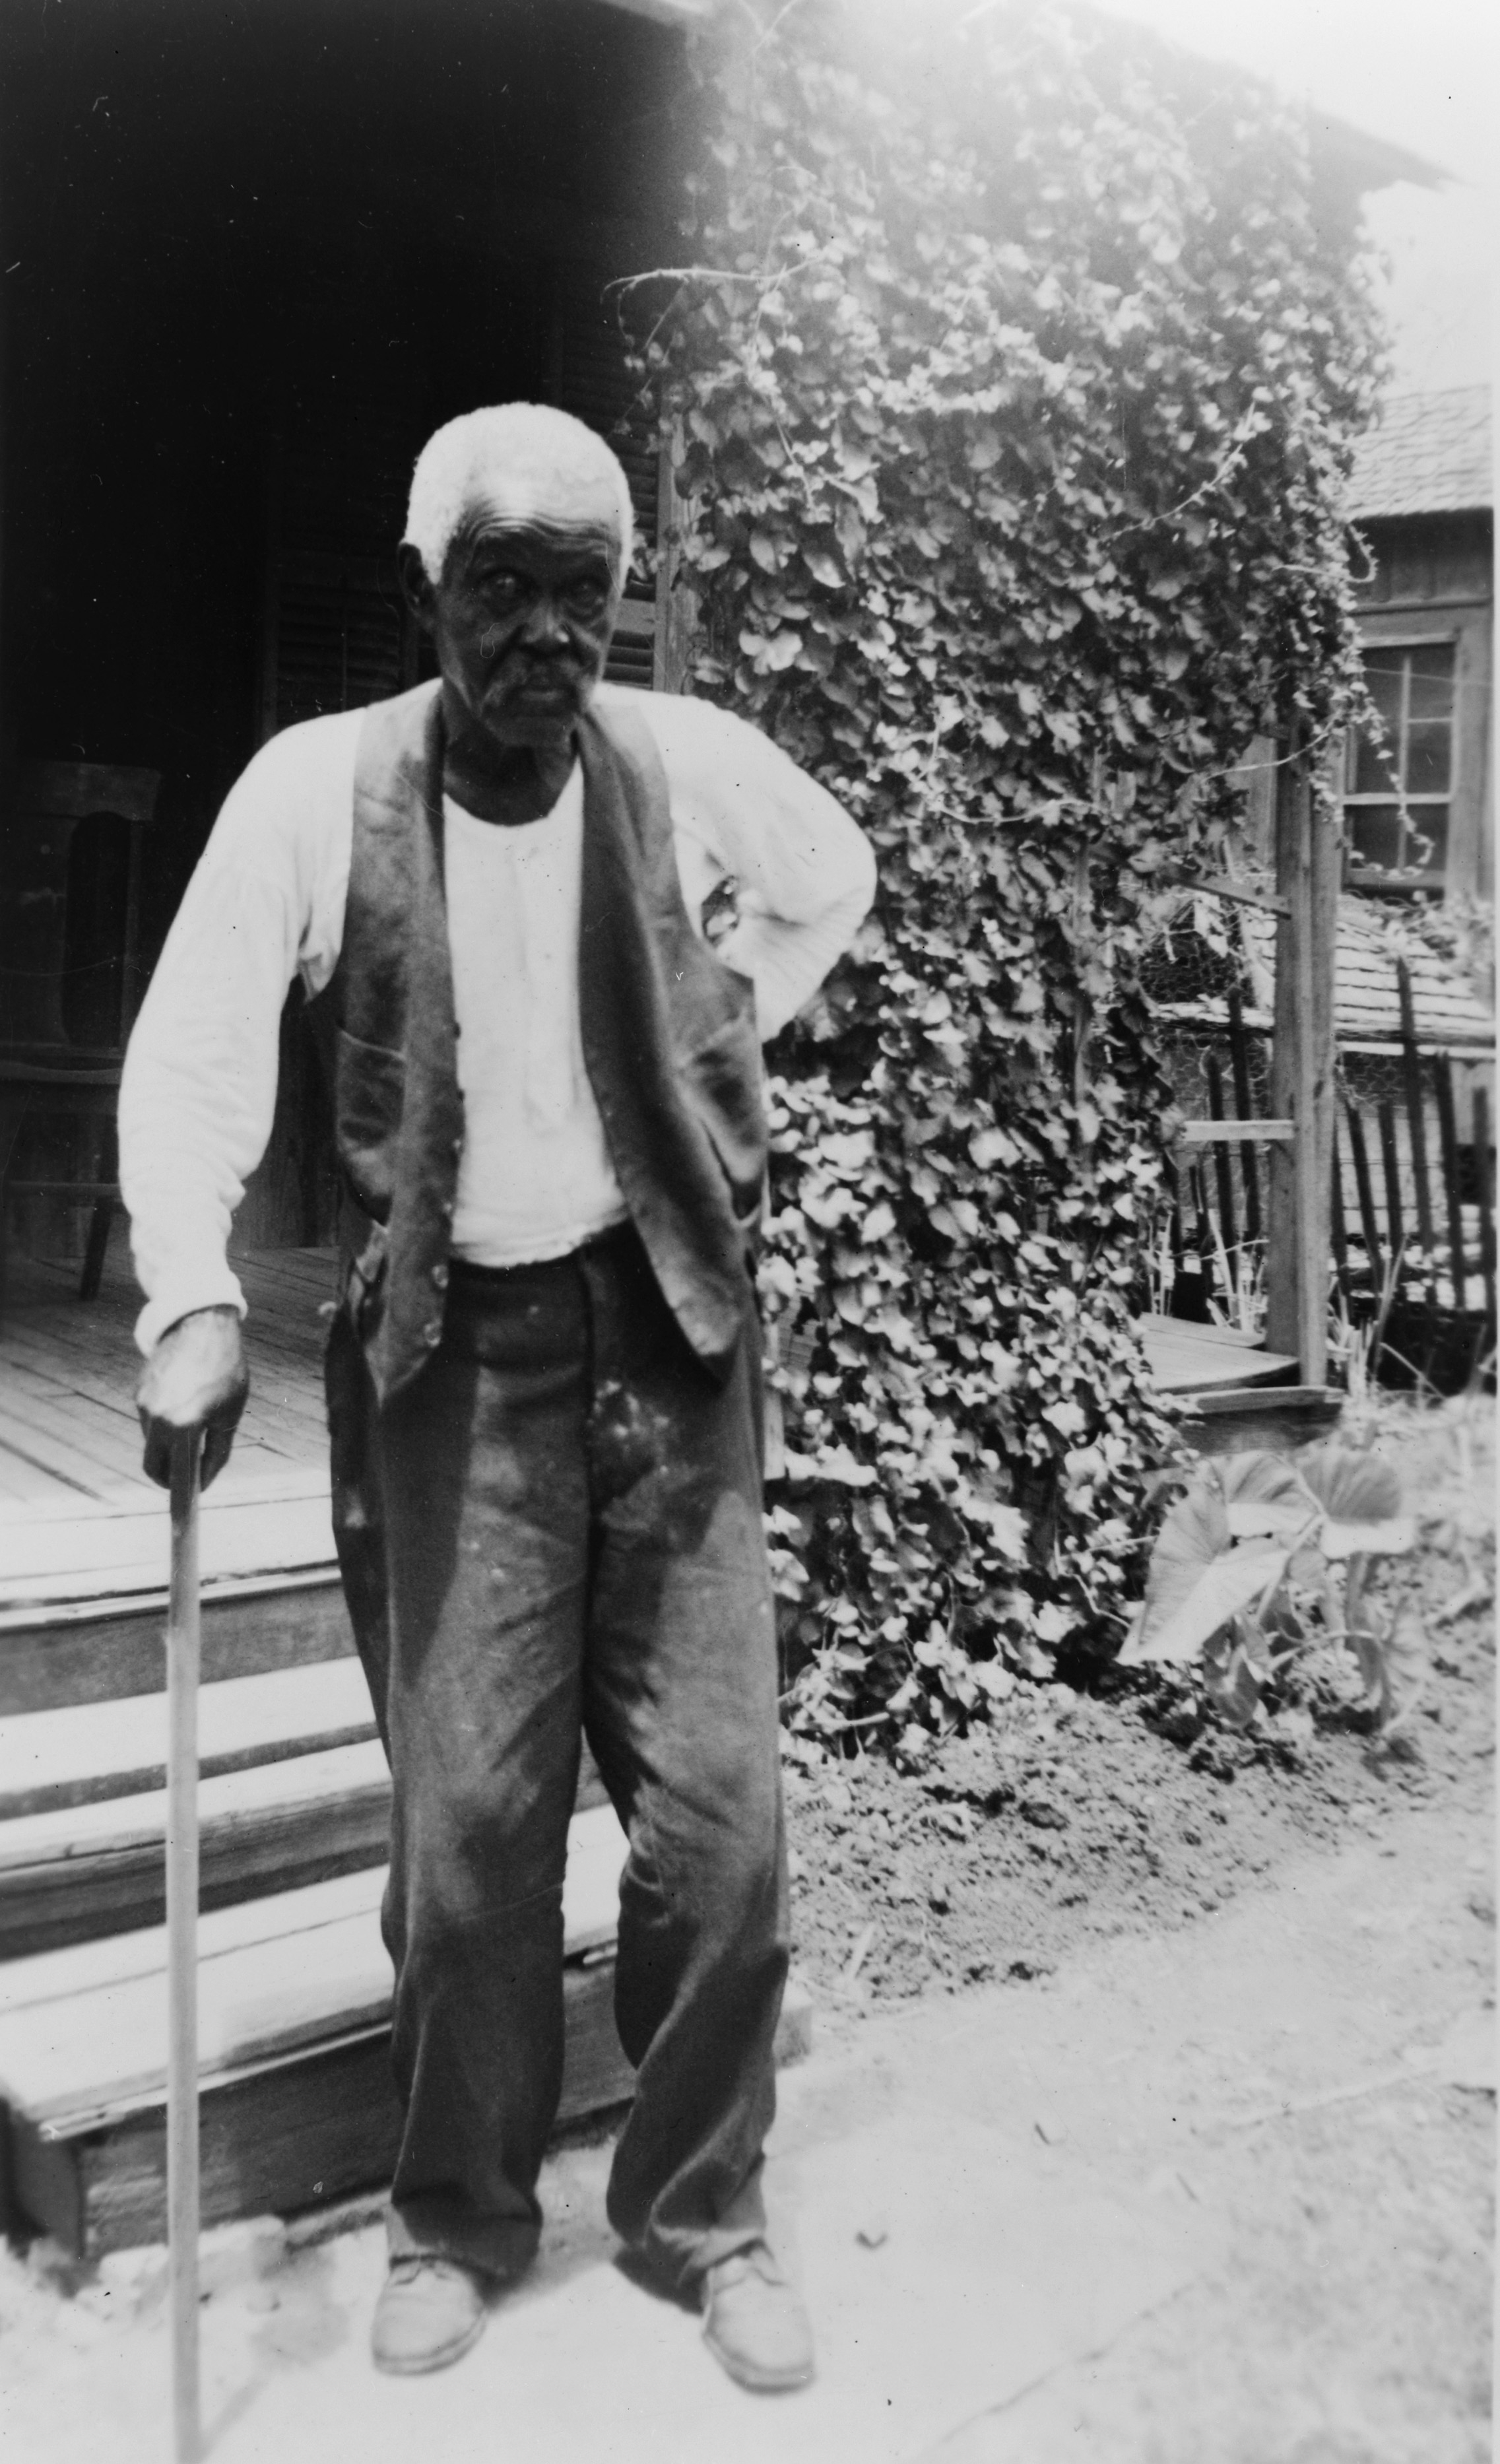
\includegraphics[width=90mm]{./imgs/felixhaywood_recorte2.jpg} \label{img21}
\caption{Felix Haywood}
%\end{minipage}
\end{figure}

\subsection{J. W. Terrill, narrativas do Texas, Parte~\versal{IV},~página~82}
\label{ref262}

``Quando ouvimos falar que a guerra tinha acabado e a gente estava
livre, todo mundo pulou e gritou e dançou. A senhora chorou e chorou e
nos disse que a gente estava livre e que queria que morressem todos de
fome, que ia ficar feliz, porque nos perder ia arruiná"-la. Havia um
montão de negros na cidade e a gente estavam em um zunzunzum, feito
abelhas entrando e saindo da colmeia. É como a gente era. Eu fui à
loucura, e no primeiro ano fui para o Norte, mas depois voltei para o
Texas''.

\subsection{Ed McCree, narrativas da Geórgia, Parte~\versal{III},~página~64}
\label{ref187}

``Foi um dia feliz para nós escravos quando chegou a notícia que a
guerra acabara e os brancos tinham que nos soltar. O senhor chamou seus
negros até o pátio da casa grande, mas eu não fiquei por lá para ver o
que ele tinha a dizer. Saí correndo daquele lugar, gritando o mais alto
que podia''.

\subsection{Reverendo Lafayette Price, narrativas do Texas, Parte~\versal{III},~página~204}
\label{ref215}

``Quando a notícia da rendição chegou, muitos negros começaram a
festejar e a cantar `sou livre, sou livre feito um sapo', porque o sapo
tem a liberdade de saltar em cima de uma tora e saltar para fora quando
bem entende''.

\subsection{Milly Henry, narrativas da Carolina do Norte, Parte~\versal{II},~páginas~400--404}
\label{ref141}

``Nasci escrava do Sr. Buck Boylan, em Yazoo City, Mississippi. Eu não
sei nada da minha família, só da minha avó, e ela morreu no Mississippi
durante a guerra.

O senhor Buck tinha três fazendas lá, a Mosley, a Middle e a Hill. Eu e
minha avó morávamos na fazenda Mosley. Um dia, o senhor Buck chegou e
nós vimos que ele estava morrendo de preocupação; depois de um tempo,
ele tomou coragem e nos disse? `Os yankees estão chegando para levar os
meus escravos e eu não vou deixar. Por esse motivo, estamos partindo
para a Carolina do Norte depois de amanhã e eu não quero ver ninguém
abrindo a boca para reclamar'.

Naquele dia, ele repassou os escravos e escolheu uns quinhentos para ir.
Ele me escolheu, mas minha avó ele disse que ia ficar para trás, porque
estava velha e fraca demais. Eu odiei aquilo, mas não disse nada.

Partimos de casa em carroças cobertas, com muita caminhada, e acho que
umas três semanas depois chegamos a Raleigh. Você devia ter ido junto
naquela viagem, querida. Quando acampava na beira da estrada, a gente
dormia no chão e cozinhava nossas rações na fogueira. Acho que foi uma
primavera antes da rendição, que foi na seguinte. (\ldots{})

Eu estava tirando água do poço no fim da Rua Fayetteville quando os
yankees chegaram. Vi eles descendo a rua a cavalo, os casacos azuis
reluzindo e os cavalos se empinando. Eu sabia que devia ter medo, mas
não tive, então fiquei ali parado, olhando. (\ldots{})

Os yankees foram bons para mim, mas foi muito difícil arranjar um
emprego, então eu não me dei tão bem quanto me dava antes da guerra.

Sim, senhor, eu fico contente que a escravidão acabou''.

\subsection{William Moore, narrativas do Texas, Parte~\versal{III},~página~132}
\label{ref199}

``O senhor Tom ouviu falar que iam emancipar os escravos em Selma,
{[}Alabama{]} então ele juntou as suas e os negros e veio para o Texas.
Mamãe disse que vieram em carroças cobertas, mas eu não tenho idade para
lembrar nada disso''.

\begin{figure}[]
%\begin{minipage}{0,4\textwidth}
\centering
 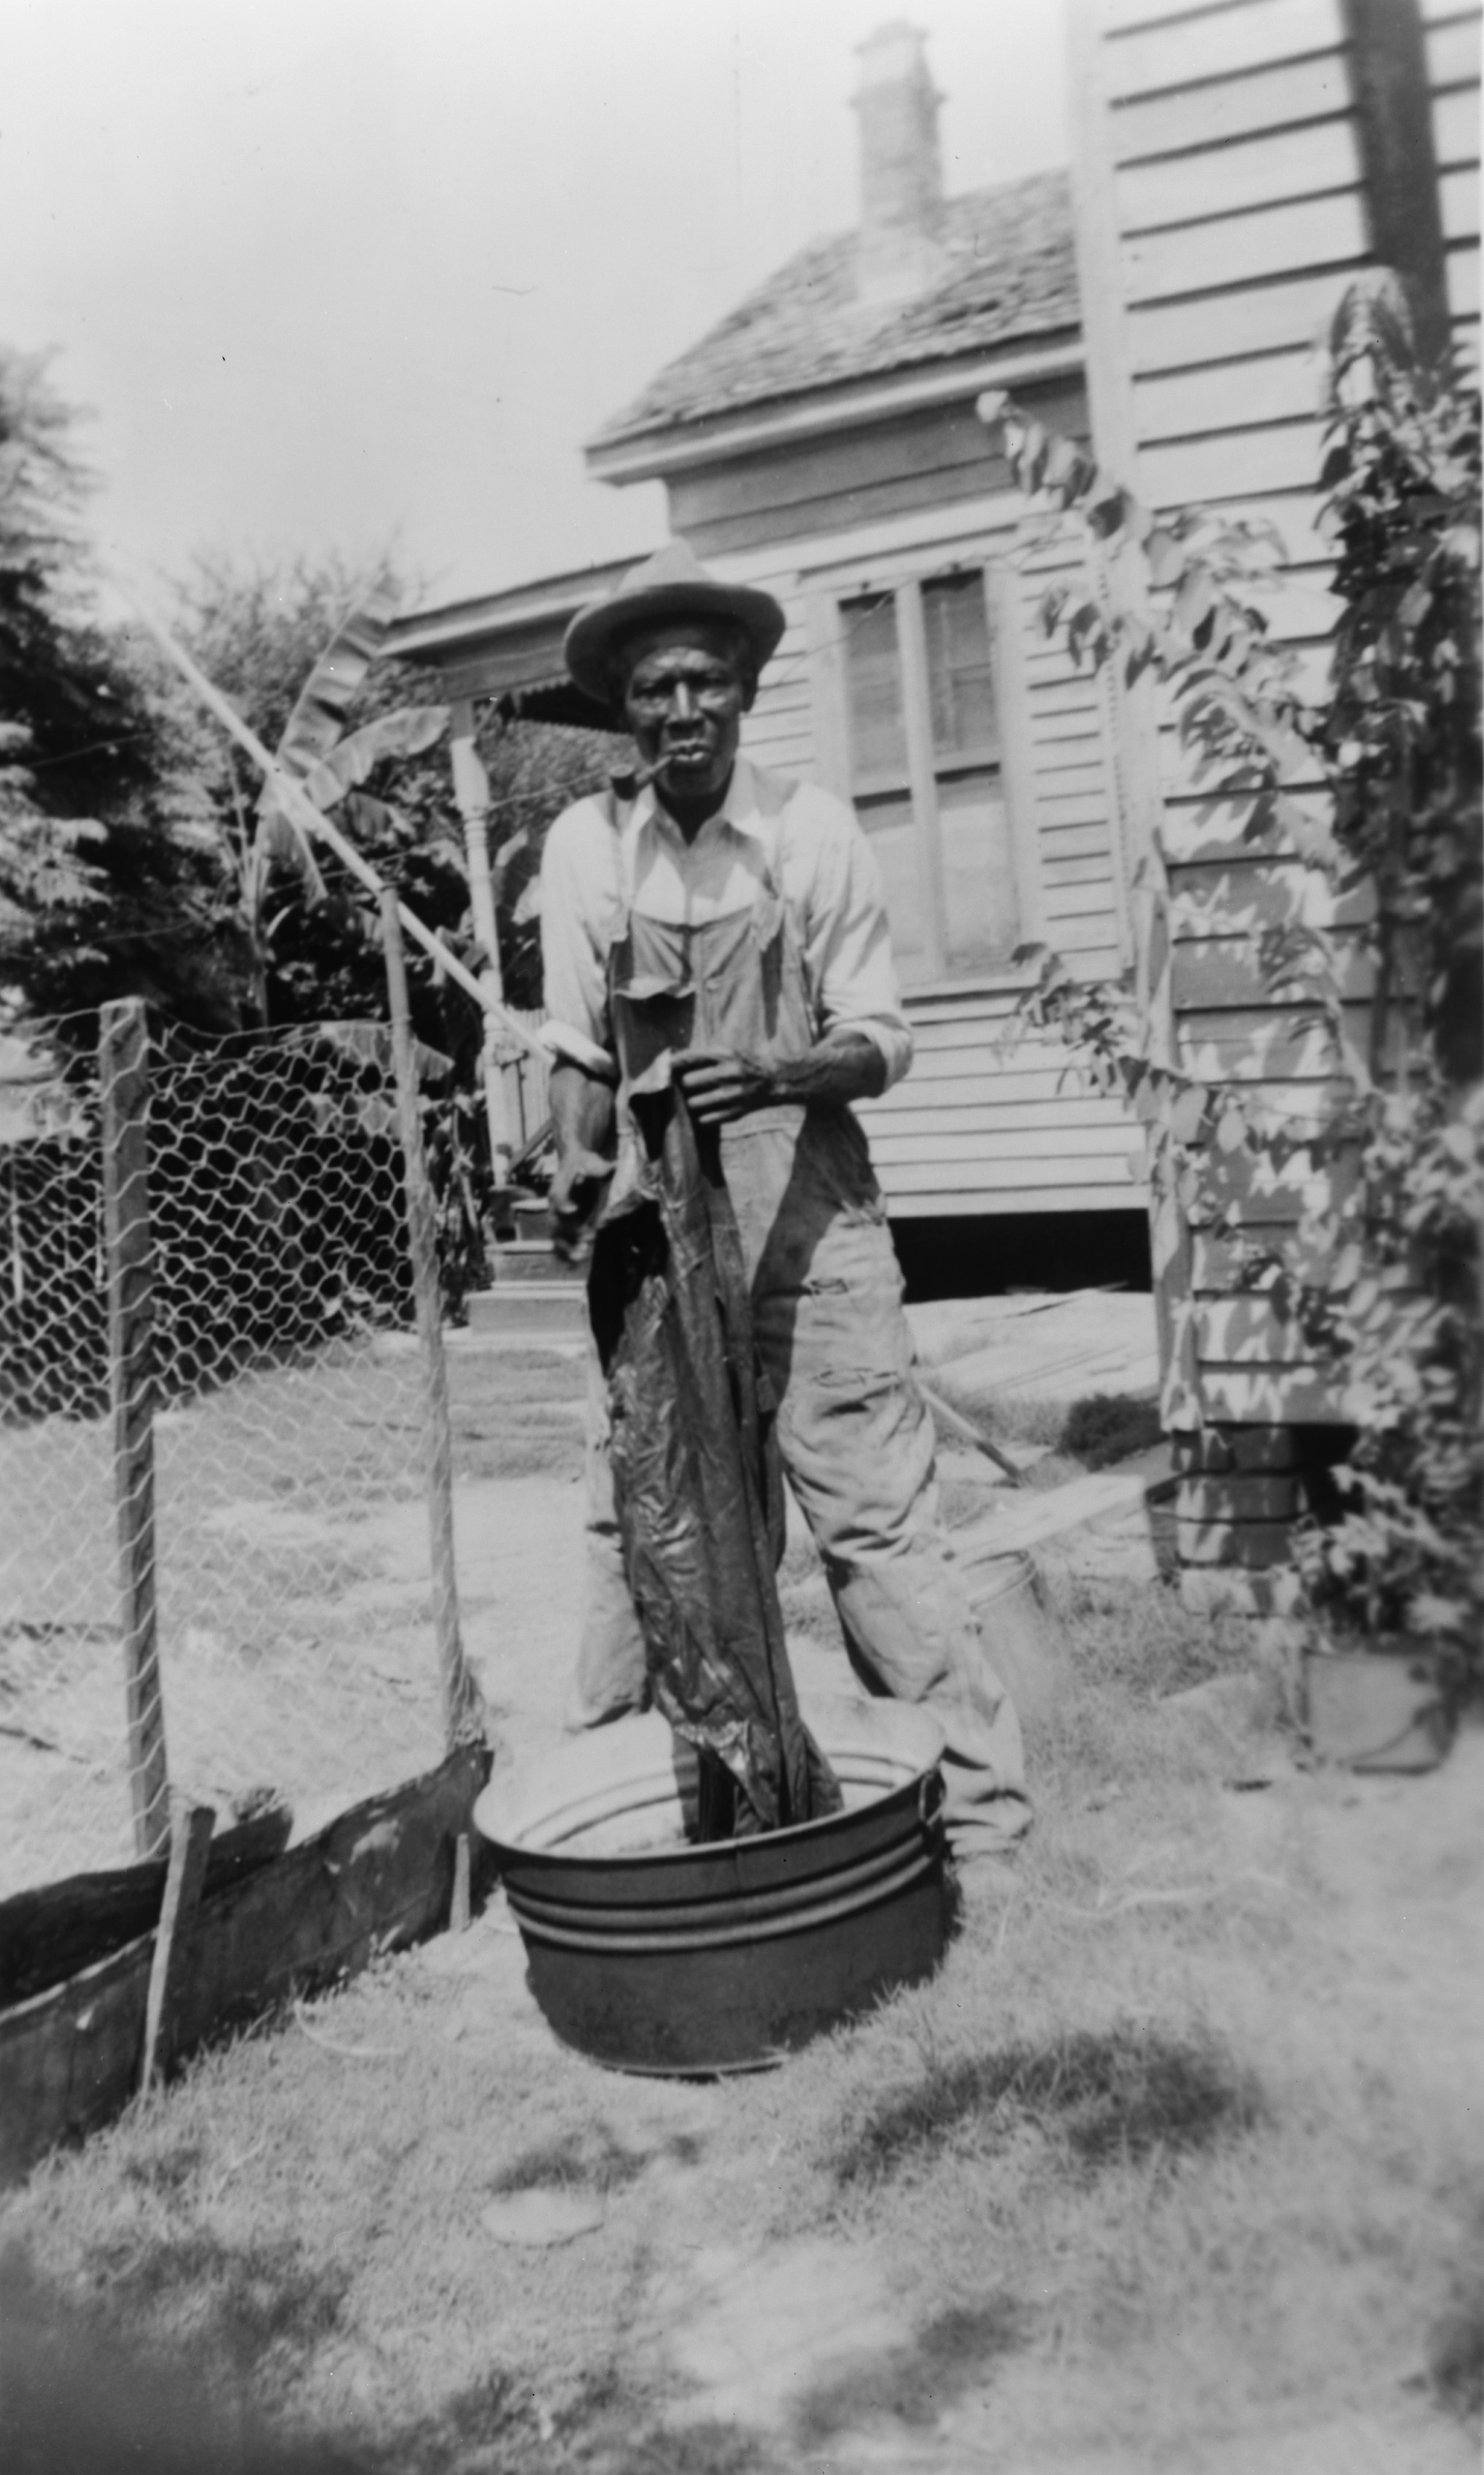
\includegraphics[width=90mm]{./imgs/vanmoore_recorte.jpg} \label{img22}
\caption{Van Moore}
%\end{minipage}
\end{figure}

\subsection{Van Moore, narrativas do Texas, Parte~\versal{III},~página~129}
\label{ref196}

``Mamãe me contou assim como foi que os Cunningham e os McKinney vieram
para o Texas. Quando a guerra começou, a maior parte de quem tinha
escravos lá na Virgínia se mudou mais para o Sul, e vários para a
Luisiana e o Texas, porque diziam que os yankees nunca iam chegar tão
longe e não iam ter que libertar os escravos se chegassem até aqui. Além
do mais, tinha muitos escravos fugindo para o Norte naquelas bandas.
Mamãe diz que quando partiram para cá nas carroças, os brancos disseram
para os coitados dos negros, que eram tão ignorantes que acreditavam em
tudo que os brancos diziam, que eles estavam indo para onde os lagos
eram cheios de xarope e cobertos de bolo de massa mole e onde não teriam
que trabalhar tanto. Eles diziam isso para ninguém fugir. (\ldots{})

Quando a guerra estourou, os soldados da União tinham um acampamento não
muito longe de nós e eu me escapulia para lá quando a velha senhora
estava distraída, pois os soldados me davam café preto e açúcar para
levar para mamãe. Eu tinha que caminhar com areia pelos joelhos para
chegar naquele acampamento. Várias outras crianças iam também, mas nunca
vi crueldade dos soldados. Eles estendiam o balde de açúcar e quando
você colocava a mão lá dentro, dava para sentir a água, porque não era
açúcar refinado como se tem agora. Mas o gosto era bom, bom mesmo''.

\subsection{Elisabeth Sparks, narrativas da Virgínia, página 52}
\label{ref252} 

``Shep foi para a guerra, mas não por muito tempo. Ele não viu nada
dela, mas os escravos sabiam qual era o motivo da guerra. Depois que ela
terminou, tentaram enganar os escravos e queriam manter eles
trabalhando, mas os yankees contaram que eles estavam livres. Mandaram
alguns escravos para a Carolina do Sul quando os yankees chegaram
perto, para não deixar os yankees pegarem eles. Mandaram meu primo James
para a Carolina do Sul. Nunca vou esquecer de quando os yankees
passaram. Eles foram levando todo o gado e todos os escravos homens para
Norfolk consigo para acabar com o sistema, os brancos por aqui iam só
continuar a ter escravos. Os escravos queriam liberdade, mas tinham medo
de dizer isso para os brancos. Bem, os yankees estavam dando tudo para
os escravos''.

\subsection{Annie Row, narrativas do Texas, Parte~\versal{III},~página~260}
\label{ref231}

{[}Quando a guerra começou:{]} ``O senhor Charlie xingou tudo e todo mundo e
nós abrimos o olho e ficamos longe dele. Dois anos depois, ele recebeu
uma carta do senhor Billy dizendo que ia voltar para casa em breve e que
Johnny tinha sido morto {[}ambos eram filhos de Charlie{]}. A senhora
começou a chorar e o senhor deu um pulo e começou a praguejar contra a
guerra, então ele pegou um atiçador em brava e disse: `Libertar os
negros, é isso que querem? Deixa que eu liberto'. E ele bateu na minha
mãe no pescoço. Ela começou a chorar e a gemer e caiu no chão. Lá
estavam, a senhora de luto, mamãe de luto e o senhor berrando o mais
alto que podia. Ele tirou a arma da parede e saiu em direção ao eito
onde os negros estavam trabalhando. Minha irmã e eu vimos isso e saímos
correndo e gritando, porque a gente tinha irmãos e irmãs no eito. Mas o
Bom Deus se fez sentir nessa confusão e o senhor não tinha ido longe
campo adentro quando caiu de repente. A morte caiu sobre ele e os negros
vieram correndo. Ele não conseguia falar nem se mexer, então carregaram
ele de volta para a casa. O doutor veio e no dia seguinte o senhor
morreu''.

\subsection{Katie Rowe, narrativas do Oklahoma, páginas~275--76,~281--83}
\label{ref232}

``{[}O senhor{]} chegou a cavalo e disse para o velho Saunders, o
feitor, que era para reunir todos nós ao redor do líder da linha, que
era meu próprio Tio Sandy, e então passou o sermão!

`Crioulos, vocês andam vendo os soldados confederados passando por aqui
esfarrapados e machucados e cansados', ele disse, `mas isso não quer
dizer que foram derrotados!'

`Os yankees não vão chegar tão longe, mas se chegarem eles não vão
libertar nenhum de vocês, porque eu mesmo vou libertar todo mundo antes
disso. Quando chegarem aqui, todo mundo já vai estar livre, porque eu
vou enfileirar vocês na margem do rio Bois d'Arc e libertar todos com a
minha espingarda! Quem deixar para trás um golpe de enxada ou um passo
da linha ou um repique do sino ou um toque da corneta vai estar livre e
conversando com o diabo muito antes de avistar um par de calça azul que
seja!'

Era assim que ele falava com a gente e assim que agia com a gente o
tempo todo''.

\subsection{Louisa e Sam Everett, narrativas da Flórida, página 130} \label{ref85}

``Louisa e Sam ouviram esse sino tocar pela última vez no outono de
1865. Todos os escravos se reuniram em frente à casa grande, onde
foram informados que estavam livres, por ora. Eles haviam ouvido boatos
sobre a guerra, mas não entendiam o significado de tudo aquilo. Agora
`Big Jim' estava chorando na varanda, amaldiçoando o destino que lhe
fora tão cruel e lhe roubara todos os seus `crioulos'. Ele indagou se
alguém queria permanecer até a colheita terminar e, quando ninguém
consentiu com isso, teve um acesso de fúria; ele sacou sua pistola e
começou a disparar contra a multidão de negros amedrontados. Alguns
morreram na hora, outros ficaram aleijados pelo resto da vida. Por fim,
ele foi convencido a parar, mas então tentou tirar a própria vida.
Alguns escravos assustados prometeram ficar com ele por mais um ano, o
que o acalmou. Foi necessário que soldados da União visitassem a fazenda
mais uma vez antes que `Big Jim' permitisse a partida de seus
ex"-escravos''.

\subsection{Ella Washington, narrativas do Texas, Parte~\versal{IV},~páginas~132--33}
\label{ref279}

``Ouvi todo mundo dizer que tinha uma guerra e meu tio e meu primo
fugiram para o escritório central, onde estavam os yankees. Mamãe diz
que era em Milligan, Texas. Quando a liberdade estava chegando na
Luisiana, eles nos refugiaram para o Texas, nas carroças. Viajamos o dia
inteiro e metade da noite e dormimos no chão. Não demorou muito para
chegar em Calvert, lá no meio do Texas, e eles nos botaram na fazenda
dos Barton. Estávamos escavando batatas por lá quando os yankees
chegaram em duas carroças enormes e nos mandaram sair da plantação e nos
libertaram. Não teve comemoração nenhuma. O senhor disse que todo mundo
podia ficar uns dias até decidir o que queria fazer.

Mas daí aconteceu uma coisa esquisita. Os escravos bebiam de um poço
velho. Eles bebiam a água de manhã, tinham umas dores de barriga
horríveis na hora do almoço e de noite estavam mortos. Morreram feito
moscas, tão rápido que não deu para fazer caixão para todos, só
costuraram uns sacos e enterraram assim mesmo. Alguns escravos dizem que
o senhor jogou veneno no poço. Não sei do que eles morreram, mas que foi
esquisito, foi''.

\subsection{Douglas Dorsey, narrativas da Flórida, página 98} \label{ref72}

``Douglas diz que nunca vai se esquecer uma noite quando tinha 14 anos
de idade, quando lhe mandaram dizer ao capataz para levar todos os
escravos até a casa. Logo, todo a escravaria de cerca de 85 escravos
estava reunida, alguns sentados em cepos, outros de pé. O filho do
coronel ficou visivelmente comovido ao anunciar que estavam todos
livres. Ele disse que poderiam ir aonde quisessem, pois ele não tinha
mais relação alguma com eles, ou que poderiam permanecer e ter para si
metade de tudo que fosse cultivado na fazenda. Os escravos ficaram
contentes com a notícia, pois mal sabiam que uma guerra estava sendo
travada.

Ninguém aceitou a oferta do coronel de permanecer, pois todos ficaram
muito contentes com a oportunidade de abandonar as crueldades da fazenda
dos Matair''.

\subsection{Irella Battle Walker, narrativas do Texas, Parte~\versal{IV},~página~124}
\label{ref272}

``Uma manhã, o senhor Washington nos chamou e leu do jornalzão. Ele
disse: `Vocês estão livres para viver e livres para morrer e livres para
irem para o diabo, se quiserem'. Ele disse que fizéssemos a sua
colheita, receberíamos pelo serviço, então deu as costas e foi embora,
chorando. Todas as famílias ficaram, exceto um homem''.

\subsection{Siney Bonner, narrativas do Alabama, páginas 40--41} \label{ref29}

``Mamãe diz que eu tinha quinze anos na época da rendição. Lembro muito
bem. O senhor John chamou todos os negros da fazenda em volta dele na
casa grande e disse para eles: `Agora vocês são livres como eu, não sou
mais o senhor de ninguém. Tentei ser bom para você e tomar conta de
todos vocês. Todos que quiserem ficar são bem"-vindos, vamos todos
trabalhar juntos e ganhar a vida. Se não quiser ficar, quem for embora
vai ter que se virar feito porco no mato'. Alguns ficaram e alguns foram
embora''.

\subsection{Randolph Johnson, narrativas do Alabama, página 231}
\label{ref164}

``Então veio a guerra, e todas as roupas boas que a gente fez no tear
viraram farrapos. A comida escasseou; alguns dos escravos fugiram,
algumas das nossas casas os yankees botaram fogo. Depois da guerra, o
senhor voltou e nos disse que os negros não eram mais escravos. Disse
que a gente podia ir, mas que quem quisesse ficar também podia. Ele deu
a cada família que ficou uma mula, uma vaca, umas ferramentas e
dinheiro, o suficiente para cuidar delas até a colheita terminar. Nunca
negro nenhum teve senhor melhor que ele''.

\subsection{Janie Gallman, narrativas da Carolina do Sul, Parte~\versal{II},~página~97}
\label{ref97} 

``Seu pai e mãe eram ambos propriedade de Bill Keenan, que era um bom
senhor. Ela nunca viu nenhum dos escravos ser açoitado e jamais viu
qualquer escravo acorrentado. Quando ela, o pai e a mãe foram
libertados, ela afirma: `Meu senhor deu para o meu pai um barril de
farinha grossa, uma vaca e um bezerro e um vagão de milho quando nos
soltou. Ele deu o mesmo para cada um dos seus escravos. Ele tinha uma
fazenda grande. Não sei quantos hectares de terra era, mas era bem
grande'".

\subsection{Tempie Herndon Durham, narrativas da Carolina do~Norte,~Parte~I,~páginas~289--90}
\label{ref77}

``Fiquei feliz quando a guerra terminou, porque daí eu e o Exter
podíamos ficar juntos o tempo inteiro, em vez de só sábado e domingo.
Depois de livres, moramos um tempão lá mesmo na fazenda do senhor
George. Alugamos a terra por um quarto do que fazíamos, e depois de um
tempo compramos uma fazenda. Pagamos 300 dólares que tínhamos
economizado. Tínhamos um cavalo, um boi, uma vaca e dois porcos, além de
algumas galinhas e quatro gansos. A senhora Betty foi até o sótão e nos
deu uma cama e uma capa de colchão e pena de ganso o suficiente para
fazer dois travesseiros, além de uma mesa e algumas cadeiras. Ela também
nos deu uns pratos. O senhor George deu para o Exter um alqueire de
semente de milho e um pouco de semente de trigo, depois mandou ele ir
até o celeiro e pegar um saco de semente de algodão. Pegamos tudo isso e
então arrumamos a carroça, arrebanhamos a criançada e se mudamos para a
nossa nova fazenda. As crianças foram colocadas para trabalhar no campo;
elas cresceram no eito, porque eram colocadas para trabalhar desde que
aprendiam a caminhar direito.

Não tem nada de errado com a liberdade, mas os negros estavam melhores
antes da rendição, porque cuidavam deles e não se metiam em confusão,
brigando e matando como fazem hoje em dia. (\ldots{}) Pode ser que o
senhor e a senhora de todo mundo não fosse bom igual o senhor George e a
senhora Betsy, mas eles eram iguais a pai e mãe para os negros deles''.

\subsection{Mack Mullen, narrativas da Flórida, páginas 238--39}
\label{ref204}

``Liberdade: Mullen lembra vividamente do dia em que ouviram a notícia
da sua emancipação; os disparos das armas ecoaram pelas florestas e
fazendas; após algum tempo, os soldados `yankees' vieram e informaram
que estavam livres. O Sr. Snellings não resistiu e não foi molestado. Os
escravos, ao ouvirem as boas novas sobre a liberdade, começaram a cantar
e rezar a Deus espontaneamente. Foi um dia de festa. Ninguém trabalhou
por uma semana, o tempo foi gasto com comemorações. O senhor disse aos
seus escravos que estavam livres e poderiam ir aonde quisessem, ou que
poderiam permanecer com ele se assim o desejassem. A maioria dos seus
200 escravos se recusou a abandoná"-lo, pois ele era considerado um bom
senhor''.

\subsection{Jerry Boykins, narrativas do Texas, Parte I, página 122} \label{ref30}

``Lembro bem de quando meu senhor {[}um rico proprietário no Condado de
Troupe, Geórgia{]} foi para a guerra. Ele chamou todos nós na cozinha e
disse que ia para lá dar uma sova naqueles filhos da puta e que ia
voltar antes do café da manhã. Ele não voltou por dois anos. `Senhor, o
seu café da manhã ia ter demorado', eu disse. `Sim, eles são os filhos
da puta mais difíceis de surrar que já vi na vida', ele respondeu.

Quando a guerra terminou, ele nos reuniu e anunciou que a gente estava
livre. `Agora eu vou dar para vocês um dia de festa', ele disse.
`Depois, vocês podem ficar e trabalhar por salário ou podem ir embora'.
Então nós puxamos dois barris de uísque e matamos uns porcos e armamos
um festão''. {[}Jerry Boykins partiu pouco depois, tendo recebido uma
oferta de emprego no Kentucky.{]}

\subsection{Willis Winn, narrativas do Texas, Parte~\versal{IV},~página~205}
\label{ref305}

``Depois da rendição, o senhor libertou os homens e a senhora libertou
as mulheres, mas ele não nos soltou quando devia. Não teve fazenda
nenhuma dividida com os negros que eu tenha ouvido falar. Os negros da
Luisiana dizem que a Rainha Elizabeth mandou um barco cheio de ouro para
a América, para dar para os libertos, mas eu nunca vi nada disso. O
senhor deu para cada um de nós um barril de farinha grossa, um barril de
farinha fina, uma costela de carne e 40 litros de melaço e nos mandou
trabalhar para quem a gente quisesse. Papai comprou duas vacas, um
cavalo, oito porcos e um bode do senhor, a crédito, e nós nos mudamos e
plantamos três safras diferentes.

Os yankees ficaram na Luisiana por bastante tempo depois da rendição.
Eles foram até as casas dos brancos que não libertaram seus escravos e
arrebentaram os barris de farinha e queimaram a carne. `Se a gente tiver
que ver vocês de novo, vamos acabar com todo mundo, do berço para cima',
eles diziam''.

\paragraph{Comentário}\quad
{\small
A decisão mais importante que os escravizados enfrentaram ao
conquistar sua liberdade era se deveriam abandonar a fazenda e buscar
trabalho em outro lugar ou ficar com um senhor conhecido. Dado o
histórico da escravidão e a realidade do racismo, não era uma decisão
simples. Os libertos sabiam que a sociedade do pós"-guerra não
estaria disposta a apoiá"-los ou ansiosa para ajudá"-los. Eles precisavam
estimar se teriam um destino melhor com a pessoa branca que conheciam ou
com um desconhecido. Em ambos os casos, eles não esperavam sempre
receber tratamento justo. Em geral, os senhores mais cruéis perderam a
maior parte da sua mão de obra assim que a guerra acabou.

Para alguns emancipados, seria preciso enfrentar uma última
batalha antes de descartarem os grilhões da escravidão. Em muitos
estados sulistas, os ex"-senhores usaram os tribunais locais para
transformar as crianças negras em ``aprendizes''. Ao se converterem nos
seus tutores legais, eles tentavam reter as crianças e os seus pais.
Tendo perdido seus escravizados, os fazendeiros usavam todos os meios que
pudessem inventar para manter a mão de obra nas suas terras. Assim,
alguns cativos precisaram da presença do exército da União
para conquistar sua liberdade ou qualquer uma das suas vantagens.
}

\subsection{Bert Strong, narrativas do Texas, Parte~\versal{IV},~páginas~71--72}
\label{ref259}

``Quando o senhorzinho foi para a guerra, chamaram todos os escravos
para se despedirem dele. (\ldots{}) Quando a guerra terminou, ele voltou
para casa e disse para o velho senhor: `Você não leu a proclamação para
os seus negros ainda?' O senhor disse que não, então o senhorzinho tocou
o berrante e nos chamou, então disse que a gente era livre igual a ele e
podia trabalhar para quem quisesse, mas que gostaria que ficássemos até
o fim da colheita. Ele disse que ia nos contratar e assinar um contrato.
Eu e mamãe ficamos dez anos, porque eles eram tão bons que não adiantava
nada ir embora''.

\subsection{Alice Green, narrativas da Geórgia, Parte~\versal{II},~página~45}
\label{ref110}

``Um dia, nós as crianças estávamos brincando no montinho de areia e
olhamos para cima e enxergamos um bando de yankees vindo para nós. Tinha
tantos deles que parecia uma revoada de passarinho azulão. Antes de irem
embora, tinha gente que achava que estavam mais para diabos azuis. Mamãe
estava na cozinha e a velha senhora disse: `Olhe pela janela, Milly; os
yankees estavam vindo e vão libertar vocês e roubar você e seus filhos
de mim. Não me deixe! Por favor, Milly, não me deixe!' Os yankees
invadiram o pátio. Eles abriram o defumadouro, o galinheiro, a tulha de
milho e tudo mais naquela fazenda. Eles levaram o que quiseram e nos
disseram que o resto era nosso para fazer o que a gente bem entendesse.
Disseram que a gente era livre e que tudo que tinha na fazenda pertencia
a nós, então foram embora e a gente nunca mais viu eles.

Quando a guerra terminou, a velha senhora chorou e chorou e implorou
para a gente não ir embora, mas nós fomos''.

\subsection{Delia Garlic, narrativas do Alabama, página 132} \label{ref101}

``Sim, senhora, o senhor Garlic tinha dois meninos na guerra. Quando
eles partiram, o senhor e a senhora choraram, mas a gente ficou feliz de
ver eles chorarem. Eles nos faziam chorar tanto.

Quando a gente soube que estava livre, todo mundo quis ir embora''.

\subsection{George Lewis, narrativas da Geórgia, Parte~\versal{III},~página~50}
\label{ref175}

{[}Viveu em situação de escravidão em Pensacola, Flórida.{]} ``Quando a guerra estourou, o Sr. Lewis afirma que costumava escutar os
mais velhos cochichando entre si à noite. (\ldots{}) Todos os escravos
na fazenda ficaram muito contentes ao ser informados de que eram livres,
mas não houve nenhuma grande demonstração, pois tinham certo receio do
que o seu senhor poderia fazer. Alguns permaneceram na fazenda, enquanto
outros partiram assim que foram informados de que eram livres''.

\subsection{George Womble, narrativas da Geórgia, Parte~\versal{IV},~página~192}
\label{ref312}

``Depois que os escravos foram libertados, diversos deles foram postos
sob obrigação de permanecer, afirma o Sr. Womble. Ele próprio teve que
permanecer com a família Womble até atingir 21 anos de idade. Quando o
dia chegou, o Sr. Womble se recusou a deixá"-lo partir. Contudo, a Sra.
Womble ajudou"-o a fugir, mas ele foi visto e pego uma noite, na casa de
uma senhora branca idosa com quem fizera amizade. Uma corda foi presa ao
redor do seu pescoço e ele foi forçado a correr todo o caminho de volta
à fazenda, enquanto os outros cavalgavam. Após mais alguns meses de
maus"-tratos, ele fugiu novamente. Desta vez, ele foi bem"-sucedido
(\ldots{})''

\subsection{Sra. Annie Price, narrativas da Geórgia, Parte~\versal{III},~páginas~182--83}
\label{ref214}

``Seu pai fugiu uma vez para escapar de um açoite (isso ocorreu durante
a Guerra Civil). Ele conseguiu escapar dos cães, além dos perseguidores
humanos. Quando questionada sobre o resultado final dessa fuga, a Sra.
Price respondeu que seu pai permaneceu oculto até a guerra terminar e
ele poder apresentar"-se sem nada a temer. (\ldots{}) Quando a Sra.
Kennon os informou que estavam livres para partirem ou ficarem, como
quisessem, seu pai, que acabara de voltar do esconderijo, disse à Sra.
Kennon que não gostaria de permanecer na fazenda por mais tempo do que
fosse necessário para reunir sua família. Ele afirmou que desejava sair
por conta e sentir como era ser livre. A Sra. Price diz que, jovem como
era, sentiu"-se muito feliz, pois o jugo do cativeiro desaparecera e ela
sabia que poderia ter privilégios como qualquer outra pessoa. Assim, ela
e sua família se mudaram e seu pai começou a lavrar a terra por conta
própria''.

\subsection{John Van Hook, narrativas da Geórgia, Parte~\versal{IV},~página~90}
\label{ref265}

``Quando a guerra terminou, o Sr. Love reuniu seus escravos e disse que
eles haviam sido libertados. Ele lhes explicou tudo com muito cuidado e
disse que poderia arranjar para que todos os que quisessem permanecer
com ele trabalhar na fazenda. Muitos dos negros foram embora depois que
ouviram falar de gente enriquecendo com o trabalho nas ferrovias do
Tennessee e sobre os altos salários sendo pagos nas grandes fazendas do
Mississippi. Alguns desses agentes de mão de obra eram incrivelmente
espertos quando se tratava de exagerar a verdade''.

\subsection{Fanny Randolph, narrativas da Geórgia, Parte~\versal{III},~página~196}
\label{ref221}

``A guerra veio chegando de pouco em pouco, e todos os homens foram
embora para lutar contra os yankees, então as mulheres e as crianças
tiveram uma vida difícil, porque todos nós tínhamos que cuidar dos
animais e trabalhar no eito. Depois a gente ouviu como os yankees
estavam por todo lado, matando as mulheres de susto dentro de casa e
fazendo elas cozinharem para eles comerem, depois destruindo e
bagunçando as casas e então indo embora.

Quando a velha Mistie ouviu dizer que os yankees estavam vindo, ela
chamou os negros para levar toda a louça, a prataria e as joias que
pertenciam à velha senhora e sua família e cavar uns buracões atrás do
defumadouro e embaixo da casa grande e deixar tudo enterrado até os
yankees passarem.

Foram dias sombrios, mas um tempão depois que a guerra terminou e
disseram que a gente era livre, eu não quis deixar meus brancos, então
fiquei com eles algum tempo (\ldots{})''.

\subsection{Anna Parkes, narrativas da Geórgia, Parte~\versal{III},~página~162}
\label{ref209}

``Eu tenho estudado sobre os tempos da guerra e lembro que o velho
senhor ficou muito preocupado com os seus negros quando ouviu falar que
uma multidão de soldados yankees estava vindo para Athens {[}na
Geórgia{]}. Diziam que os yankees iam escolher os melhores negros para
levar consigo e havia muita falação sobre o jeito escandaloso como os
soldados yankees estavam tratando as negras, mulheres e meninas. Antes
de chegarem aqui, o velho senhor mandou a maioria dos seus melhores
negros para Augusta {[}a 150 quilômetros de Athens{]}, para não correrem o risco
de serem pegos pelos federais. Contudo, os negros que ele manteve não
foram nada incomodados, porque os federais respeitavam o juiz e não
fizeram nada de mal nas suas terras. (\ldots{}) O velho senhor mandou
nos chamar depois que a guerra acabou, e a gente ficou muito orgulhoso
de voltar para casa''.

\subsection{Shade Richards, narrativas da Geórgia, Parte~\versal{III},~página~204}
\label{ref224}

``O Sr. Jimmy levou Shade para a guerra consigo. Shade precisou atuar
como seu criado pessoal e também cuidar dos dois cavalos. As balas
perfuraram o casaco e o chapéu de Shade muitas vezes, mas `o Senhor
estava tomando conta' dele e ele nunca se machucou. Eles estavam na
batalha de Appomatox e `na rendição' em 8 de abril de 1865, mas `as
evidências não foram compromissadas até 29 de maio, então esse é o dia
em que os negros comemoram a emancipação'.

O irmão de Shade ajudou a construir a ferrovia de Atlanta a Macon para
que os soldados e a munição dos confederados pudesse ser transportada
com mais rapidez.

Naquele tempo, um negro não era adulto até fazer 21 anos, por maior que
fosse. Shade estava `praticamente' crescido quando a guerra terminou,
mas trabalhou para o Sr. Neal por quatro anos. Seus pais alugaram um
terreno, mula e arado do Sr.~Neal e a família ficou reunida. No início,
eles davam aos negros apenas um décimo do que plantavam, mas isso não
era o suficiente para sobreviver e após `muito bate"-boca sobre o
assunto', eles passaram a receber um terço. Isso também não bastava para
sobreviver, então o `bate"-boca' continuou até darem a metade, `e é isso
que se ganha até hoje'".

\subsection{Adeline Willis, narrativas da Geórgia, Parte~\versal{IV},~página~166}
\label{ref299}

``Quando questionada sobre a guerra, Tia Adeline diz que a vida era
muito mais difícil naquela época. `Ora, a gente não tinha sal, nem sal,
e não se arranjava naqueles tempos. A gente tinha que recolher a terra
do defumadouro onde a carne pingava e fazer correr feito barrela para
poder salgar as coisas. Sim, senhora, a vida era difícil e nosso senhor
passou na guerra todos os quatro anos e a gente tinha que fazer o melhor
que podia. Nós não íamos saber nada se não por uma negrinha velha e
desbocada na senzala que vivia falando em `liberdade'. Ela incomodou
muito os nossos brancos, era muito desbocada com eles, mas não venderam
e ela foi libertada junto com a gente. Quando todos voltaram para casa
da guerra e o senhor nos chamou e disse que a gente estava livre, alguns
ficaram tão felizes que gritaram, mas outros não; ficaram tristes. Lewis
{[}seu marido{]} veio correndo, ele queria que eu e as crianças fôssemos
morar na fazenda dos brancos dele com ele, mas eu não quis. Não,
senhora, eu não queria deixar os meus brancos para trás. Mandei o Lewis
seguir em frente e me deixar em paz, eu conhecia meus brancos e eles
eram bons para mim, mas não conhecia os brancos dele. Então a gente
continuou a viver como vivia na escravidão, mas ele vinha me ver todos
os dias. Depois de alguns anos, ele finalmente me convenceu a ir até a
fazenda dos Willis para morar com ele, e os brancos dele foram muito
bons para mim'".

\subsection{Sarah Gudger, narrativas da Carolina do Norte, Parte~I,~páginas~357,~358}
\label{ref116}

``Na fazenda tinha uma velha que o chefe comprara de um bando da
Virgínia. O chefe comprou ela de um dos especuladores. Ela riu e nos
disse: `Qualquer dia desses você vão todos ser livres, igual aos
brancos', mas todos rimos dela. Não, nós somos só escravos, sempre temos
que trabalhar e nunca vamos ser livres. Quando a liberdade chegou, ela
disse: `Eu disse, agora vocês não aprenderam nada, não têm nada, não têm
casa; o que é vão fazer? Eu não disse?' (\ldots{})

Quando a guerra terminou, o senhor William disse: `Vocês sabem que são
livres? Pois são livres agora'. Eu dei uma risadinha, lembrando do que a
velha nos dissera sobre liberdade sem ter aprendido nada. Vários homens
queriam que eu fosse para o estrangeiro, mas eu respondi que ia morar
com meu pai enquanto ele vivesse. Fiquei com os brancos uns doze meses,
depois fiquei com papai enquanto ele viveu''.

\subsection{Molly Harrell, narrativas do Texas, Parte~\versal{II},~páginas~116--17}
\label{ref122}

``Todo mundo falava em liberdade e rezava para ser livre antes de
morrer. Lembro da primeira vez que os yankees passaram, minha mãe me pôs
em cima da cerca. Eles costumavam passar com sacolas nas mulas que
enchiam com coisas das casas. Eles entravam no celeiro e se serviam.
Entravam nos estábulos e soltavam os cavalos dos brancos e espantavam
tudo que não levavam para eles.

Uma noite, lembro muito bem, eu e minha mãe estávamos sentadas na
choupana, prontas para ir dormir, quando ouvimos alguém chamando ela.
Escutamos o feitor cochichar por baixo da porta e dizer para mamãe que
ela era livre, mas para não contar para ninguém. Não sei por que ele fez
isso. Ele sempre gostou de mamãe, então acho que fez por ela. O senhor
nos leu os papéis logo depois disso e falou que estávamos livres.

Mamãe e eu partimos na mesma hora {[}da fazenda, no Texas{]} para
Palestine {[}uma cidade próxima da fazenda{]}. Quase todo mundo foi com
a gente. Todos caminhamos estrada afora, cantando e gritando ao som da
música. Meu pai veio no dia seguinte e se juntou a nós. Minha irmã
nasceu lá. Depois fomos para Houston e Luisiana por um tempo e eu fui
trabalhar de cozinheira. Trabalhei até virmos para Galveston, uns dez
anos atrás''.

\subsection{Martin Ruffin, narrativas do Texas, Parte~\versal{III},~página~267}
\label{ref234}

``O senhor não contou que a gente estava livre por três ou quatro dias
depois da liberdade, então disse: `Vocês estão livres; não vão embora,
eu vou pagar vocês'. Primeiro os negros não entenderam o que ele queria
dizer, então alguém falou: `Estamos livres, acabou o chicote e as
surras'. Você devia ter visto eles pulando e batendo palmas e dançando.

Mamãe e papai foram embora trabalhar para si mesmos em uma fazenda, mas
eu fiquei para trás até estar quase crescido''. {[}Nesse caso, o senhor de
escravos provavelmente foi aos tribunais para obter a tutela legal do
escravo menor de idade.{]}

\subsection{Adeline White, narrativas do Texas, Parte~\versal{IV},~página~154}
\label{ref282}

``O velho senhor não foi para a guerra e os meninos dele eram pequenos
demais. Só ouvimos falar da guerra e que ela ia nos libertar. De noite,
a gente escapulia para o mato e fazia um culto, rezando para a liberdade
chegar rápido. A gente tomava bastante cuidado, porque o senhor ia
açoitar todo mundo se descobrisse. Ficávamos fora quase toda a noite,
dormindo e rezando, dormindo e rezando. Quando finalmente chegou a
notícia da liberdade, o senhor disse que todo mundo estava livre para ir
embora, mas para quem ficasse ele ia pagar. A maioria se foi, porque o
senhor era bem malvado e se a gente não precisa ficar, não fica, não com
aquele senhor''.

\begin{figure}[]
%\begin{minipage}{0,4\textwidth}
\centering
 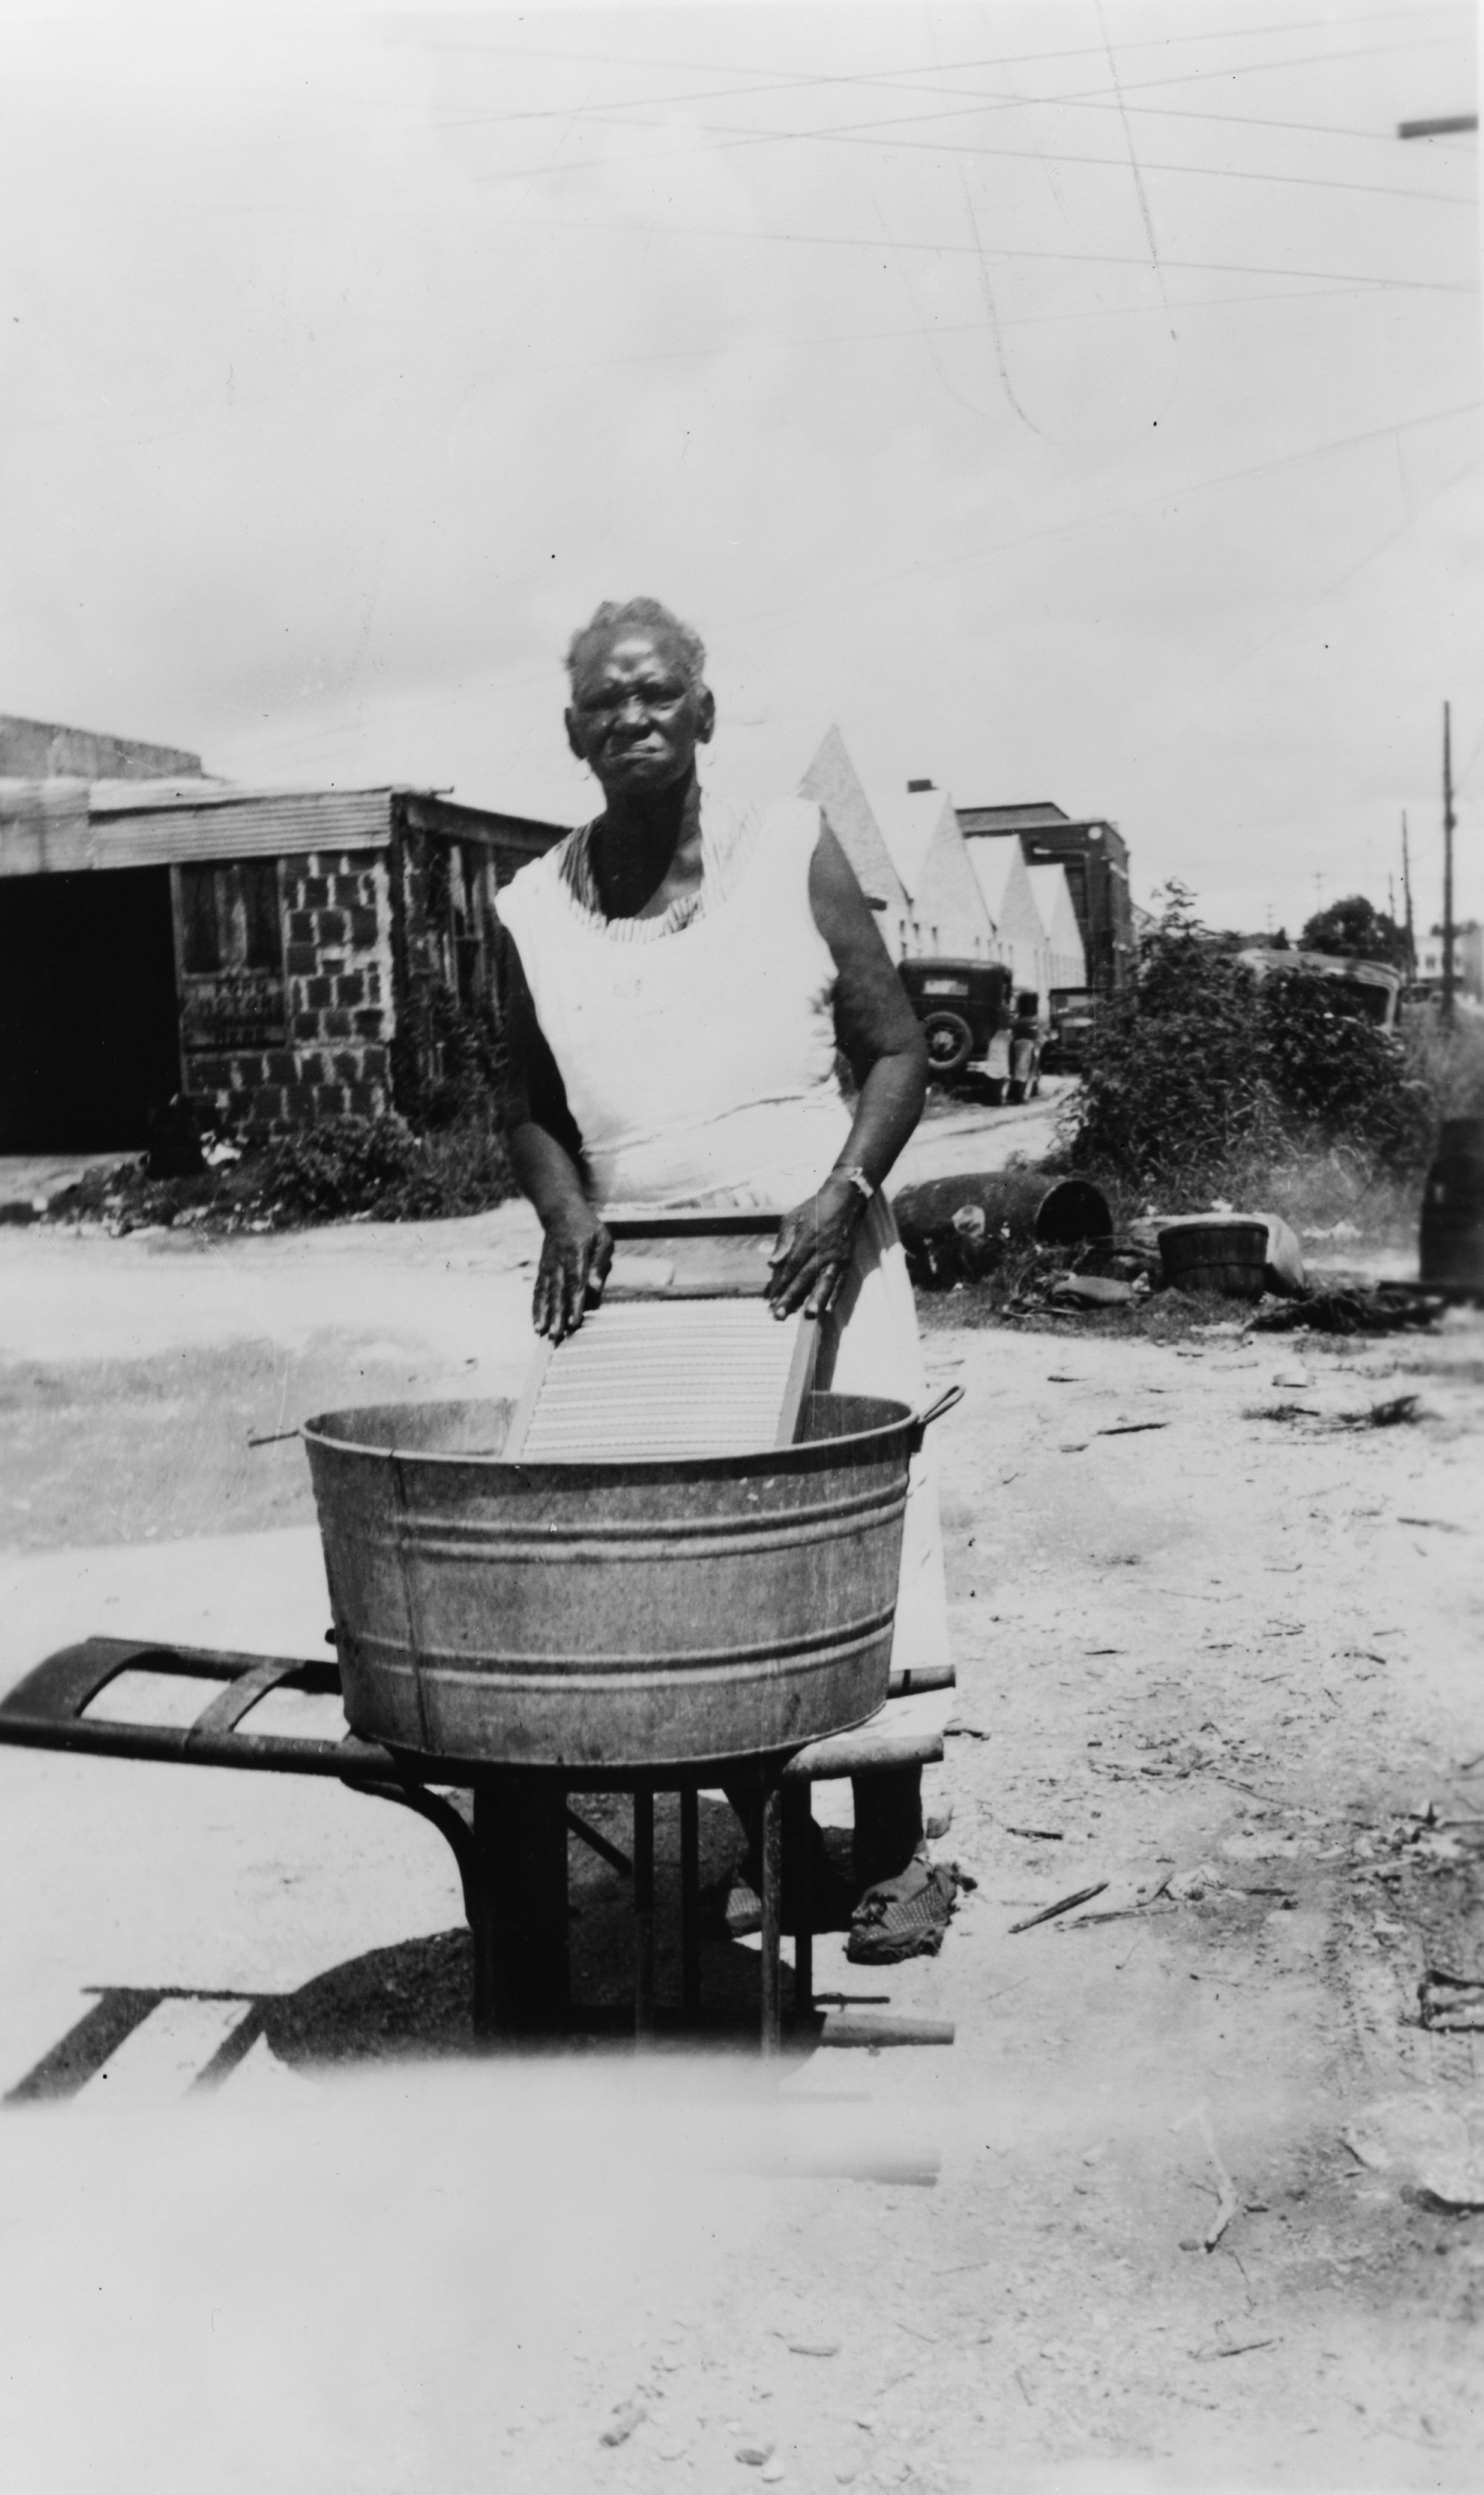
\includegraphics[width=90mm]{./imgs/adlinewhite_recorte.jpg} \label{img23}
\caption{Adeline White}
%\end{minipage}
\end{figure}

\subsection{Sra. Betty Guwn, narrativas do Indiana, página 99} \label{ref117}

``Quando a Guerra Civil começou, houve uma grande agitação entre nós
escravos {[}numa fazenda perto Canton, Kentucky{]}. Estávamos sob
vigília cerrada, especialmente como soldados para os dois exércitos. Meu
marido fugiu cedo e ajudou Grant a tomar o Forte Donaldson. Ele disse
que libertaria a si mesmo, o que fez; mas quando finalmente fomos
libertados, toda nossa família se preparou para partir. O senhor nos
implorou para ficar e ofereceu dois quilos de farinha grossa e um quilo
de faceira de porco toda semana se ficássemos para trabalhar. Nós fomos
todos morar em Burgard, Kentucky''.

\subsection{Joe Higgerson, narrativas do Missouri, página 178}
\label{ref144}

``Quando disseram que os negros eram livres, o chefe veio e leu os
papéis para eles dizendo que eram livres. E eu fui para Boonville
{[}Missouri{]} e me alistei no Exército da União, em 23 de novembro de
1863. Servi no 25º Corpo de Exército, Segunda Divisão, sob o General
Whitsell. Eu lutei na última batalha da guerra, em Palmetto Ranch,
Texas, no rio Grande, a apenas 58 quilômetros do Golfo. Quando recebi baixa do
exército e voltei para casa, pensei: ora, eu não tenho casa, para onde
vou? Então decidi voltar para Boonville. Minha família tinha toda se
espalhado''.

\paragraph{Comentário}\quad
{\small
Nas últimas fases da guerra, a passagem das tropas do Norte por
diversas plantações em 1864 e 1865 foi motivo para festa. A liberdade
estava chegando. Mas a chegada das tropas também significava que os
escravizados precisavam ser cautelosos e tomar muito cuidado para evitar
riscos futuros. Por mais felizes que estivessem ao ver os soldados,
também sabiam que as forças invasoras seguiriam em frente e que
logo o proprietário voltaria a ser a força dominante na fazenda.

Isso significa que mesmo um ato de bondade das tropas podia
colocar os escravizados em uma situação difícil. Se os soldados yankees
abriam o defumadouro e davam carne ou comida para eles, estes
podiam ter que enfrentar o senhor enfurecido um ou dois dias depois,
depois que os soldados fossem embora. Infelizmente, os soldados nem
sempre tratavam os cativos bem. Muitas tropas dos estados do Oeste eram
famosos pelo racismo ferrenho, e além disso às vezes tinham fome e se
ressentiam das privações sofridas durante a guerra. Esses soldados
muitas vezes abatiam o gado ou roubavam tudo que pudesse dar algum
conforto às suas vidas. Essas ações prejudicavam o bem"-estar dos
escravizados, apesar de a liberdade ser uma benção que todos desejavam
ardentemente.
}

\subsection{Callie Williams, narrativas do Alabama, páginas 426--27}
\label{ref290}

``Quando veio a rendição, ela diz que um regimento inteiro de soldados
cavalgou até a casa, gritando para os negros que eles estavam livres.
Depois, os soldados levaram a carne do defumadouro e distribuíram todo o
melaço e a farinha entre os negros. Eles roubaram as abelhas e depois
almoçaram e foram à próxima fazenda, levando os homens com eles, todos
exceto os que eram velhos demais, papai entre eles''.

\subsection{Anderson Edwards, narrativas do Texas, Parte~\versal{II},~página~8} \label{ref81}

``Lembro que quando a guerra começou, George, o filho do senhor,
encilhou o velho Bob, seu pônei, e foi embora. Ele ficou fora seis
meses. `Como vai a guerra, George?', o senhor perguntou quando ele
chegou de volta. `É o inferno', o senhor George disse. `Bob e eu estamos
se batendo com os yankees desde o começo'. Antes da guerra, o senhor
nunca falou nada sobre a escravidão, mas quando ouviu falar que
estávamos livres, ele praguejou e disse: `Deus nunca pretendeu libertar
os negros', e seguiu praguejando até morrer. Mas ele não nos contou que
estávamos livres até um ano inteiro depois da liberdade, mas um dia um
bando de soldados yankees apareceram e o senhor e a senhora se
esconderam. Os soldados entraram na cozinha, onde mamãe estava batendo
leite, e um deles chutou a desnatadeira. `Vai embora, você é livre igual
a mim'. Então eles saquearam a fazenda e quebraram janelas. Quando foram
embora, parecia que tinha passado uma tempestade naquela casa. O senhor
saiu do esconderijo e foi quando começou a praguejar e a berrar e
continuou até o dia em que morreu''.

\subsection{Sam Word, narrativas do Arkansas, Parte~\versal{VII},~página~240}
\label{ref315}

``Minha mãe tinha muitas coisas bonitas, colchas e tudo mais, que
guardava em um baú da sua cabaninha. Um dia, um soldado yankee escalou a
janela dos fundos e levou algumas das colchas. Ele enrolou elas e estava
saindo do pátio quando minha mãe enxergou ele. `Seu salafrário de uma
figa! Vocês dizem que vieram para cá lutar pelos negros, mas agora estão
roubando deles'. `Mentirosa maldita!', ele respondeu volta. `Eu estou
lutando por 14 dólares por mês e pela União'".

\subsection{Carolina Richardson, narrativas da Carolina do Norte, Parte~\versal{II},~páginas~199--201} \label{ref225}

``Não se ouviu muito sobre a guerra, não como se ouviu sobre a Guerra
Mundial. Sei que ninguém da nossa fazenda foi para a guerra, porque o
senhor Ransome era velho demais e o senhor George era patrulheiro, ou
talvez fosse só jovem demais. Falava"-se um pouquinho, mas da maioria não
se ouviu. Eu cuidava dos bebês escravos, mas mamãe cozinhava na casa
grande ouviu um pouco de conversa sobre a guerra e eu escutei ela
falando com papai sobre o assunto. Quando me viu escutando, ela disse
que ia cortar minha orelha fora se contasse para alguém. Eu tinha visto
alguns dos escravos com as orelhas cortadas e queria ficar com as
minhas, então não disse nada.

Um dia, a senhora Betsy veio no pátio e disse para as crianças: `Vocês
têm o hábito de correr até o portão para ver quem vai ser o primeiro a
dizer oi para as nossas visitas, mas os yankees vão chegar hoje ou
amanhã e eles não são nossas visitas. Na verdade, se correrem até o
portão para recebê"-los, eles vão atirar em vocês'.

No final da noite, eu ouvi música e corri até o portão para ver quem
era. Descendo a estrada o mais rápido que podiam, vi um bando de homens
em casacos cinzas, cavalgando feito o demônio. Eles não pararam na nossa
casa, mas mais tarde ouvi dizer que eram a cavalaria do Wheeler, o pior
de todos os rebeldes, se bem que dizem que em batalha eram corajosos.

Uma hora depois que o bando do Wheeler passou, avistou"-se os yankees. Os
tambores estavam rufando, as bandeiras tremulavam, os cavalos se
empinavam bem alto. Os negros tinham sido ensinados que os yankees
queriam nos matar, homem, mulher e criança. Todos nós, todos os cento e
poucos, correram para se esconder.

Sim, senhora, eu lembro dos uniformes azuis e dos botões de latão, e
lembro de como entraram pelo portão dizendo que a guerra estava quase
vencida e que deviam enforcar os homens do Sul que não tinham ido para a
guerra.

Acho que falaram bem grosso com o senhor Ransome. Bem, mamãe disse para
o capitão yankee que ele devia ter vergonha de falar com um velho
daquele jeito. Além do mais, ela disse que se era assim que iam lhe dar
a liberdade, ela não queria nada disso. Com isso, mamãe levou a senhora
Betsy para cima, onde os yankees não iam ficar de olho nela.

Um dos yankees me achou e perguntou quantos pares de sapato eu ganhava
por ano. Eu disse que ganhava um par. Então ele me perguntou o que eu
vestia no verão. Quando disse para ele que não vestia nada além de uma
camisa, e que passava o verão descalça, ele soltou uns palavrões
horríveis e xingou meu senhor.

Mamãe disse que falaram que ela e papai iam ganhar um pouco de terra e
uma mula se nos libertasse. Pois veja, eles tentaram voltar os escravos
contra os seus senhores.

Com a rendição, a maioria dos negros foi embora, mas eu e a minha
família ficamos para ganhar salário''.

\subsection{Henry Lewis, narrativas do Texas, Parte~\versal{III},~páginas~11--12}
\label{ref177}

``O velho senhor morreu antes da guerra, então o filho dele, John Cade,
assumiu a fazenda, com a ajuda dos irmãos. Eles se chamavam Overton,
Taylor e Bob Jr. Todos nós queríamos ser livres e conversávamos sobre
isso entre nós na senzala, mas não se dizia nada onde os brancos fossem
nos escutar.

Quando a guerra chegou, eu via soldados todos os dias. Eles estavam
acampados em Liberty e eu ficava observando eles. Também ouvi as armas,
talvez em Sabine Pass, mas não vi nada de luta. Foi um ano comprido para
se esperar, aquele último ano da guerra. Mandaram os papéis em 5 de
março, pelo que ouvi, mas não nos soltaram naquele dia. Este aqui foi o
último estado a libertar os escravos. Quando não soltaram eles em março,
os soldados yankees vieram em junho e fizeram eles nos soltar. Na manhã
depois que os soldados vieram, o feitor leu os papéis e disse que a
gente estava livre como ele e podia ir. Alguns ficaram na antiga fazenda
um tempão, outros foram embora''.

\subsection{Spencer Barnett, narrativas do Arkansas, Parte~I,~páginas~117--18} \label{ref19}

``Os yankees queimaram a casa grande. Era uma casa bonita. A velha
senhora se mudou para a casa do feitor. Ele era um homem branco. Ele se
mudou para outro lugar. Os yankees fizeram ataques, em um deles levaram
15 ou 20 bezerros de uma só vez. Botaram fogo no depósito de batatas.
Levaram o milho. A velha senhora chorou mais de uma vez. Os yankees
mataram de fome mais negros do que brancos com essa roubalheira. Depois
da guerra, os escravos tinham dificuldade para arranjar abrigo e comida
o suficiente no inverno. Morreram pilhas deles depois daquele agosto que
lhe falei''.

\subsection{Anne Bell, narrativas da Carolina do Sul, Parte~I,~página~53} \label{ref23}

``Eu tinha uns dez anos quando os yankees vieram. Eles estavam
transbordando de maldade. Tiravam os vestidos dos armários e vestiam e
davam risada. Antes de irem embora, eles pegavam tudo. Levaram a carne e
os mantimentos do defumadouro e o melaço, o açúcar e a farinha fina e
grossa da casa. Mataram os porcos e as vacas, botaram fogo no
descaroçador e no algodão e roubaram o gado, os gansos, as galinhas e os
perus''.

\subsection{Violet Guntharpe, narrativas da Carolina do Sul, Parte~\versal{II},~páginas~216--17}

``Os yankees nos atiraram no meio da sarça, mas a gente não nasceu e
cresceu lá feito um coelho. A gente nasceu em uma bela casa de madeira.
As vacas estavam lá no canavial para nos dar leite, os porcos estavam
engordando com noz de hicória, bolotas e milho debulhado para nos dar
carne e banha; os carneiros davam lã, o algodão no descaroçador estava
lá para nos dar roupas. Os cavalos e as mulas estavam lá para ajudar com
o milho e o algodão, mas quando os yankees vieram e levaram tudo embora,
a gente só podia agradecer a eles era pela barriga vazia, e pela
liberdade''.

\subsection{Anderson Bates, narrativas da Carolina do Sul, Parte~I,~página~43} \label{ref20}

``Eu tinha quinze anos quando os yankees passaram. Eles levaram tudo:
cavalos, mulas, vacas, ovelhas, bodes, perus, gansos e galinhas. Porcos?
Sim, senhor, eles mataram os porcos e levaram os pedaços que queriam,
deixavam o resto sangrando no pátio. Quando foram embora, o velho senhor
teve que ir até o Condado de Union para arranjar rações''.

\subsection{Savilla Burrell, narrativas da Carolina do Sul, Parte~I,~página~151} \label{ref40}

``Naquela fazenda, a gente esperava os yankees como hoje se espera o
Salvador e o exército dos anjos na segunda vinda. Eles chegaram em um
dia de fevereiro. Levaram tudo que podia ser carregado da fazenda e
queimaram a casa grande, os estábulos, os celeiros e o descaroçador, só
deixaram a senzala''.

\subsection{Will Sheets, narrativas da Geórgia, Parte~\versal{III},~páginas~242--43}
\label{ref238}

``Mamãe disse que a gente ia ser livre. O senhor Jeff que não ia, e ele
não nos disse o contrário até lá pelo Natal depois do abril em que a
guerra terminou. Ele disse que a gente estava livre, mas que queria que
ficasse com ele, e nenhum dos negros dele foi embora. Todos trabalharam
igual trabalhavam antes de serem libertados, só que ele pagava salário
depois da guerra.

Lembro dos yankees descendo a estrada, roubando pelo caminho. Eles
trocavam os sacos de ossos deles pelos cavalos grandes e gordos dos
brancos. Nunca vi tanto cavalo magro ao mesmo tempo na minha vida como
eles tinham. Os yankees roubaram toda a carne, as galinhas e os lençóis
bons e botaram fogo nas casas. Fizeram maldade à farta por onde
passaram. Lembro que o senhor Jeff montou um dos seus negros no seu
cavalo com um bule cheio de ouro e mandou para o meio do mato. Depois
que os yankees foram embora, ele mandou buscar de volta o ouro e aquele
cavalo bonito que tinha salvado dos soldados''.

\subsection{Barbara Haywood, narrativas da Carolina do Norte, Parte~\versal{II},~página~386}
\label{ref133}

``Os yankees levaram toda a carne do defumadouro e foram na senzala
pegar toda a carne que os brancos tinham guardado lá. Foi a primeira vez
que entrou presunto na casa dos negros. Bem, os yankees levaram todo o
presunto, mas nos deram os ombros''.

\subsection{Elbert Hunter, narrativas da Carolina do Norte, Parte~I,~páginas~459--60}
\label{ref156}

``Quando a gente ouviu falar que os yankees estavam vindo, o velho
senhor e eu levamos o gado e os cavalos para o meio do pântano e ficou
lá com eles por vários dias. Um dia, eu fui para casa e lá estavam eles,
atirando nas galinhas e nos porcos e tudo mais. Eu vi eles cortarem o
pernil de um porco vivo, ou de uma vaca e ir embora com o animal
gemendo. O senhor abateu os bichos, mas foi horrível.

Naquela noite, eles foram embora, mas no outro dia apareceu um bando
maior e mamãe cozinhou para eles o dia inteiro. Eles mataram e roubaram
tudo, e finalmente o velho senhor foi até Raleigh e pediu uma guarda.
Depois que a guarda chegou, a bagunça acabou. Um dos oficiais que passou
a noite lá perdeu a carteira com sete notas de dólar dentro, foi a
primeira vez que vi aquilo.

A gente ficou feliz com a liberdade, apesar de os nossos brancos serem
bons. O horário de trabalho era desde o sol nascer até a noite e as
mulheres tinham que cardar e fiar um certo tanto todas as noites. A
gente tinha as nossas galinhas e uma roça e dava para ganhar um pouco de
dinheiro, mas não dava para se divertir''.

\subsection{Margaret Hughes, narrativas da Carolina do Sul, Parte~\versal{II},~páginas~329--30}
\label{ref155}

``Ora, moça, já lhe contei quase tudo que eu lembro, exceto sobre os
yankees. Quando eu escutava os negros mais velhos falando sobre os
yankees que estavam vindo, eu tinha medo, porque achava que estavam
falando de algum tipo de animal. Minha tia velha ficava contente em
ouvir que os yankees estavam vindo. Ela se botava a falar sobre como ia
ser bom para a gente depois que os yankees chegassem. `Minha filha', ela
dizia, `a gente vai se dar tão bem, sentando na mesa dos brancos,
comendo na mesa dos brancos, se balançando naquela cadeirona de
balanço'. Mas aconteceu uma coisa horrível com um dos escravos quando os
yankees chegaram mesmo. Uma das meninas contou para os yankees onde a
senhora tinha escondida a prataria, o dinheiro e as joias, e eles
levaram tudo. O que você acha que aconteceu com a coitadinha? Ela fez
errado, eu sei, mas eu odiei ver ela sofrer tanto por causa daquilo.
Depois que os yankees se foram, o senhor e a senhora deixaram ela
pendurada até morrer. Foi uma coisa horrível de se ver. Os yankees
levaram tudo que a gente tinha, exceto um pouco de comida, mal o
suficiente para nos manter vivos''.

\subsection{Katie Rowe, narrativas do Oklahoma, página 281}
\label{ref233}

{[}Os yankees{]} ``vieram e levaram toda a carne, milho e batata que
quiseram. `Por que vocês não pegam toda a carne e o melaço que quiserem,
seus crioulos pobres?', eles nos diziam. `Vocês que fizeram tudo, é de
vocês tanto quanto de qualquer outro'. Mas a gente sabia que eles iriam
embora logo e que íamos apanhar se fizéssemos isso.

Alguns negros escaparam e fugiram com os yankees, mas eles tinham que
trabalhar duro igual para eles, e não comiam tão bem nem tantas vezes
com os soldados.

Nunca vou esquecer do dia em que fui libertada. (\ldots{}) Sentado na
galeria, em uma cadeira de assento de couro estava um homem que ninguém
nunca tinha visto antes. Ele estava com um chapéu bem grande, de aba
larga, como o que os yankees usavam, mas não tinha o cordão amarelo
igual ao dos yankees, e ele estava vestindo roupa de loja que não era de
fio cru nem brim, e ela era preta. (\ldots{})

O homem disse (\ldots{}) `Hoje é quatro de junho, e este é 1865, e quero
que todos vocês lembrem da data, porque sempre vão lembrar do dia. Hoje
vocês são livres, livres como eu, e como o Sr. Saunders e a sua senhora
e todos nós brancos', o homem disse. (\ldots{})

Nós só ficamos vendo ele ir pela estrada, então fomos até o Sr. Saunders
e perguntamos o que ele queria que fizéssemos. Ele só resmungou e disse
que a gente podia fazer o que bem entendesse, até onde sabia, mas que
era melhor ir embora da fazenda, a menos que alguém quisesse ficar e
trabalhar no eito por metade do que se colhesse. (\ldots{}) Mas fomos
todos enganados naquela primeira rodada! Quando a colheita terminou, a
gente não recebeu a metade!''

\paragraph{Comentário}\quad
{\small
Durante a guerra, as lideranças negras e alguns políticos do Norte
argumentaram que os libertos precisariam de terras, educação, o
direito ao voto e proteção contra brancos derrotados hostis no Sul. Sem
essas medidas, a liberdade seria uma ilusão, pois os negros continuariam
a depender dos brancos mais poderosos. A maioria dessas medidas nunca
foi integrada às políticas do Presidente Abraham Lincoln, entretanto,
pois o seu plano de Reconstrução na época em que morreu envolvia apenas
reconhecer a liberdade dos escravos e algumas disposições para a sua
educação no futuro.

No final de 1864, a ideia de terras para os libertos conquistou um
apoiador inusitado, o General William Tecumseh Sherman decretou uma
ordem militar reservando vastas quantidades de terras abandonadas ao
longo da costa do Oceano Atlântico, desde Port Royal, na Carolina do
Sul, até o rio São João, no norte da Flórida, estendendo"-se mais de 60
quilômetros a Oeste. Sherman estava planejando a sua última campanha militar,
saindo de Savannah, Geórgia, em direção às Carolinas, e não queria ser
onerado pelos milhares de escravizados fugitivos que seguiriam o seu
exército, como aconteceu na Geórgia. A Ordem de Operações Especial \#15
de Sherman foi a origem de ``40 acres e uma mula''. A ideia se
disseminou rapidamente entre os escravizados, que ansiavam desesperadamente
por terras, que por sua vez serviriam de base para a sua independência
econômica e social. Não demorou para que 40 mil afro"-americanos se
estabelecessem nas terras demarcadas por Sherman.

Antes do final de 1865, entretanto, o presidente Andrew Johnson,
sucessor de Abraham Lincoln após o assassinato, decidiu que essas terras
seriam devolvidas aos seus proprietários brancos. A intransigência dos
brancos do Sul forçou o Congresso nortista a conceder aos homens negros
o direito ao voto, mas essas conquistas logo foram revertidas; os
brancos sulistas retomaram o controle político e o Norte perdeu o
interesse pelos assuntos do Sul. Assim, é compreensível que os
ex"-escravizados expressassem sentimentos conflitantes a respeito da
emancipação quando refletiam sobre a história da sua raça.
}

\subsection{Walter Calloway, narrativas do Alabama, página 53} \label{ref43}

``Não foi muito depois que eles nos contaram que estávamos livres. Mas,
meu Deus, capitão, nós nunca fomos o que eu chamo de livre. Sim, claro,
o velho senhor não era mais o nosso dono, e toda a gente logo se
espalhou pelo mundo, mas se são todos como eu, eles ainda têm que
trabalhar duro igual, e às vezes têm menos do que a gente costumava ter
quando ficávamos na fazenda do senhor John''.

\subsection{John N. Davenport, narrativas da Carolina do Sul, Parte~I,~página~243} \label{ref67}

``Não, os escravos nunca esperaram nada quando a guerra terminou, os
nossos da vizinhança não esperavam. Tem quem fale sobre ganhar 40 acres
de terra e uma mula, mas nós nunca esperamos isso. Ninguém nunca ganhou
nada, nenhum dinheiro dos antigos senhores nem de ninguém mais''.

\subsection{Berry Smith, narrativas do Mississippi, página 132}
\label{ref242}

``Quase todos os negros que tinham donos bons ficaram com eles, mas os
outros foram embora. Alguns voltaram, outros não.

Ouvi um falatório sobre como todos os negros iam ganhar quarenta acres e
uma mula. Fizeram a gente acreditar direitinho, mas nunca vi ninguém
ganhar nada''.

\subsection{Frances Willingham, narrativas da Geórgia, Parte~\versal{IV},~páginas~159--60}
\label{ref297}

``Meu Deus, mas eu vi muito daqueles yankees indo e vindo. Eles vinham
até a casa do nosso senhor e roubavam as mulas boas. Levavam tudo que
queriam de carne, galinhas, banha e xarope e depois derramavam o resto
do xarope no chão mesmo. (\ldots{})

Eu fico muito contente que o Sr. Lincoln nos libertou. Se ainda fossem
os tempos da escravidão, velha como sou, eu ainda ia ter que trabalhar
igual, doente ou não. Agora eu não preciso perguntar para ninguém o que
eu posso fazer. É por isso que fico feliz de ser livre''.

\subsection{George Strickland, narrativas do Alabama, página 362}
\label{ref257} 

``Foi o plano de Deus libertar os negros, não de Abraham Lincoln''.

\subsection{William Pratt, narrativas da Carolina do Sul, Parte~\versal{III},~página~279}
\label{ref213}

``Acho que o que Abraham Lincoln fez não foi bem certo, porque ele
soltou todos os negros no mundo sem eles terem como se arranjar. Eles
ficaram desamparados. Ele devia ter feito aquilo gradualmente e dado a
eles a chance de se sustentarem''.
